% Options for packages loaded elsewhere
\PassOptionsToPackage{unicode}{hyperref}
\PassOptionsToPackage{hyphens}{url}
%
\documentclass[
  12pt,
]{article}
\usepackage{amsmath,amssymb}
\usepackage{lmodern}
\usepackage{iftex}
\ifPDFTeX
  \usepackage[T1]{fontenc}
  \usepackage[utf8]{inputenc}
  \usepackage{textcomp} % provide euro and other symbols
\else % if luatex or xetex
  \usepackage{unicode-math}
  \defaultfontfeatures{Scale=MatchLowercase}
  \defaultfontfeatures[\rmfamily]{Ligatures=TeX,Scale=1}
\fi
% Use upquote if available, for straight quotes in verbatim environments
\IfFileExists{upquote.sty}{\usepackage{upquote}}{}
\IfFileExists{microtype.sty}{% use microtype if available
  \usepackage[]{microtype}
  \UseMicrotypeSet[protrusion]{basicmath} % disable protrusion for tt fonts
}{}
\makeatletter
\@ifundefined{KOMAClassName}{% if non-KOMA class
  \IfFileExists{parskip.sty}{%
    \usepackage{parskip}
  }{% else
    \setlength{\parindent}{0pt}
    \setlength{\parskip}{6pt plus 2pt minus 1pt}}
}{% if KOMA class
  \KOMAoptions{parskip=half}}
\makeatother
\usepackage{xcolor}
\IfFileExists{xurl.sty}{\usepackage{xurl}}{} % add URL line breaks if available
\IfFileExists{bookmark.sty}{\usepackage{bookmark}}{\usepackage{hyperref}}
\hypersetup{
  pdftitle={Factors affecting reliablity of state-space age-structured assessment models},
  pdfauthor={Timothy J. Miller1; Andrew Applegate; Greg Britten; Elizabeth N. Brooks; Gavin Fay; Alex Hansell; Christopher M. Legault; Brandon Muffley; Brian C. Stock; John Wiedenmann},
  hidelinks,
  pdfcreator={LaTeX via pandoc}}
\urlstyle{same} % disable monospaced font for URLs
\usepackage[margin=1in]{geometry}
\usepackage{graphicx}
\makeatletter
\def\maxwidth{\ifdim\Gin@nat@width>\linewidth\linewidth\else\Gin@nat@width\fi}
\def\maxheight{\ifdim\Gin@nat@height>\textheight\textheight\else\Gin@nat@height\fi}
\makeatother
% Scale images if necessary, so that they will not overflow the page
% margins by default, and it is still possible to overwrite the defaults
% using explicit options in \includegraphics[width, height, ...]{}
\setkeys{Gin}{width=\maxwidth,height=\maxheight,keepaspectratio}
% Set default figure placement to htbp
\makeatletter
\def\fps@figure{htbp}
\makeatother
\setlength{\emergencystretch}{3em} % prevent overfull lines
\providecommand{\tightlist}{%
  \setlength{\itemsep}{0pt}\setlength{\parskip}{0pt}}
\setcounter{secnumdepth}{5}
\newlength{\cslhangindent}
\setlength{\cslhangindent}{1.5em}
\newlength{\csllabelwidth}
\setlength{\csllabelwidth}{3em}
\newlength{\cslentryspacingunit} % times entry-spacing
\setlength{\cslentryspacingunit}{\parskip}
\newenvironment{CSLReferences}[2] % #1 hanging-ident, #2 entry spacing
 {% don't indent paragraphs
  \setlength{\parindent}{0pt}
  % turn on hanging indent if param 1 is 1
  \ifodd #1
  \let\oldpar\par
  \def\par{\hangindent=\cslhangindent\oldpar}
  \fi
  % set entry spacing
  \setlength{\parskip}{#2\cslentryspacingunit}
 }%
 {}
\usepackage{calc}
\newcommand{\CSLBlock}[1]{#1\hfill\break}
\newcommand{\CSLLeftMargin}[1]{\parbox[t]{\csllabelwidth}{#1}}
\newcommand{\CSLRightInline}[1]{\parbox[t]{\linewidth - \csllabelwidth}{#1}\break}
\newcommand{\CSLIndent}[1]{\hspace{\cslhangindent}#1}
\usepackage{url}
\usepackage{setspace}
%\singlespacing
%\onehalfspacing
\doublespacing
\usepackage{lineno}
\linenumbers
\usepackage[belowskip=0pt,aboveskip=0pt]{caption}
\usepackage{relsize}
\newcommand{\Fmsy}{\ensuremath{F_{\text{MSY}}}\xspace}
\newcommand{\Fspr}[1]{\ensuremath{F_{\text{{#1}\%}}}\xspace}
\newcommand{\afrb}{Alaska Fishery Research Bulletin\xspace}
\newcommand{\ajms}{African Journal of Marine Science\xspace}
\newcommand{\amb}{Advances in Marine Biology\xspace}
\newcommand{\bms}{Bulletin of Marine Science\xspace}
\newcommand{\bjssf}{Bulletin of the Japanese Society of Scientific Fisheries\xspace}
\newcommand{\cb}{Conservation Biology\xspace}
\newcommand{\cjfas}{Canadian Journal of Fisheries and Aquatic Sciences\xspace}
\newcommand{\ea}{Ecological Applications\xspace}
\newcommand{\eer}{Evolutionary Ecology Research\xspace}
\newcommand{\elet}{Ecology Letters\xspace}
\newcommand{\emod}{Ecological Modelling\xspace}
\newcommand{\ebf}{Environmental Biology of Fishes\xspace}
\newcommand{\ff}{Fish and Fisheries\xspace}
\newcommand{\fo}{Fisheries Oceanography\xspace}
\newcommand{\fr}{Fisheries Research\xspace}
\newcommand{\fb}{Fishery Bulletin\xspace}
\newcommand{\ijms}{ICES Journal of Marine Science\xspace}
\newcommand{\iccat}{Collective Volume of Scientific Papers ICCAT\xspace}
\newcommand{\jae}{Journal of Animal Ecology\xspace}
\newcommand{\jai}{Journal of Applied Ichthyology\xspace}
\newcommand{\jdc}{Journal Du Conseil International Pour L'exploration De La Mer\xspace}
\newcommand{\jdcp}{Journal Du Conseil Permanent International Pour L'exploration De La Mer\xspace}
\newcommand{\jembe}{Journal of Experimental Marine Biology and Ecology\xspace}
\newcommand{\jfb}{Journal of Fish Biology\xspace}
\newcommand{\jsr}{Journal of Sea Research\xspace}
\newcommand{\jtb}{Journal of Theoretical Biology\xspace}
\newcommand{\jfrbc}{Journal of the Fisheries Research Board of Canada\xspace}
\newcommand{\jnwafs}{Journal of Northwest Atlantic Fisheries Science\xspace}
\newcommand{\mcf}{Marine and Coastal Fisheries: Dynamics, Management, and Ecosystem Science\xspace}
\newcommand{\mb}{Marine Biology\xspace}
\newcommand{\meps}{Marine Ecology Progress Series\xspace}
\newcommand{\mfr}{Marine Fisheries Review\xspace}
\newcommand{\mpb}{Marine Pollution Bulletin\xspace}
\newcommand{\najfm}{North American Journal of Fisheries Management\xspace}
\newcommand{\nzjmfr}{New Zealand Journal of Marine and Freshwater Research\xspace}
\newcommand{\pnas}{Proceedings of the National Academy of Sciences USA\xspace}
\newcommand{\rpvrciemm}{Rapports et Proc\`es-Verbaux des R\'eunions. Conseil Internationale pour l'Exploration de la Mer\xspace}
\newcommand{\rpvrcpiemm}{Rapports et Proc\`es-Verbaux des R\'eunions. Conseil Permanent Internationale pour l'Exploration de la Mer\xspace}
\newcommand{\rfbf}{Reviews in Fish Biology and Fisheries\xspace}
\newcommand{\sajms}{South African Journal of Marine Science\xspace}
\newcommand{\tafs}{Transactions of the American Fisheries Society\xspace}

\newcommand{\anzjs}{Australian \& New Zealand Journal of Statistics\xspace}
\newcommand{\as}{Applied Statistics\xspace}
\newcommand{\csda}{Computational Statistics \& Data Analysis\xspace}
\newcommand{\ees}{Environmental and Ecological Statistics\xspace}
\newcommand{\jas}{Journal of Applied Statistics\xspace}
\newcommand{\jabes}{Journal of Agricultural, Biological, and Environmental Statistics\xspace}
\newcommand{\jasa}{Journal of the American Statistical Association\xspace}
\newcommand{\jrssb}{Journal of the Royal Statistical Society. Series B\xspace}
\newcommand{\sm}{Statistics in Medicine}

\usepackage{xspace}
\usepackage{bm}
\usepackage{caption,graphics}
\usepackage{graphicx}
\usepackage{makecell}
\renewcommand\figurename{Fig.}
\captionsetup{labelsep=period, singlelinecheck=false}
\newcommand{\changesize}[1]{\fontsize{#1pt}{#1pt}\selectfont}
\renewcommand{\arraystretch}{1.5}
\renewcommand\theadfont{}
\usepackage{booktabs}
\usepackage{longtable}
\usepackage{array}
\usepackage{multirow}
\usepackage{wrapfig}
\usepackage{float}
\usepackage{colortbl}
\usepackage{pdflscape}
\usepackage{tabu}
\usepackage{threeparttable}
\usepackage{threeparttablex}
\usepackage[normalem]{ulem}
\usepackage{makecell}
\usepackage{xcolor}
\ifLuaTeX
  \usepackage{selnolig}  % disable illegal ligatures
\fi
\usepackage[]{natbib}
\bibliographystyle{cjfas2.bst}

\title{Factors affecting reliablity of state-space age-structured
assessment models}
\author{Timothy J. Miller\textsuperscript{1} \and Andrew
Applegate \and Greg Britten \and Elizabeth N. Brooks \and Gavin
Fay \and Alex Hansell \and Christopher M. Legault \and Brandon
Muffley \and Brian C. Stock \and John Wiedenmann}
\date{}

\begin{document}
\maketitle

\(^1\)corresponding author:
\href{mailto:timothy.j.miller@noaa.gov}{\nolinkurl{timothy.j.miller@noaa.gov}},
Northeast Fisheries Science Center, Woods Hole Laboratory, 166 Water
Street, Woods Hole, MA 02543 USA\\

\pagebreak

\hypertarget{summary}{%
\subsection*{Summary}\label{summary}}
\addcontentsline{toc}{subsection}{Summary}

We conducted a simulation study where we simulated process errors and
observations for 72 operating models with alternative assumptions about
fishing history, degree of uncertainty in index and age composition
observations, type (recruitment, survival, fishery selectivity,
catchability and natural mortality), degree of variation, and
correlation of process errors. We fit 20 different estimating models to
each of 100 simulated set of observations with alternative assumptions
type and correlation structure of process errors, (mean) natural
mortality was known or estimated, and a B-H stock recruit relationship
was assumed or not.

Across simulations we summarized probability of convergence of fitted
models, accuracy of marginal AIC in determining the correct process
error assumption and it ability to determine the Beverton-Holt stock
recruit relationship, bias in annual spawning stock biomass, in
estimation of natural mortality, and in stock-recruit relationship
parameters, and severity of retrospective patterns for estimation
models.

Alternative measures of convergence performed differently. Invertible
hessians and resulting standard error estimation was possible when
criteria based on the gradient of the optimized log-likelihood with
respect to the fixed effects parameters. Using hessian-based
convergence, probability of convergence was best for models that assumed
the correct source of process error, assumed M was known, and did not
assume stock-recruit relationships.

Using marginal AIC provided most accurate inferences about the process
errors on recruitment and survival and selectivity, in that AIC
preferred EMs with assumed process errors that matched OMs, and EMs with
those assumed process errors were not preferred when alternative process
errors were assumed in the OMs. However, when the true process errors
were more variable, AIC accuracy increased to a useful level. We found
AIC more accurately determined a B-H stock recruit relationship rather
than the null model without a S-R relationship when there was low
variability in recruitment, low variability in survival random effects,
and higher variation in spawning biomass over the time series. When the
(mean) natural mortality rate was estimated, we found large bias and
uncertainty much more likely in model output such as spawning stock
biomass.

Bias in spawning stock biomass estimation was generally low for
estimating models that assumed the correct source of process error when
there was lower observation error. Reliable estimation of stock-recruit
relationship parameters only appears possible in ideal situations with
lower observation errors in age composition and indices, lower
variability in recruitment process errors and large contrast in spawning
biomass over time. We found little evidence of bias for many OM process
error assumptions when there was contrast in fishing pressure even when
there was greater observation error although it can lead to more
variable estimates of natural mortality. For OMs where there was bias in
natural mortality due to high observation error, estimating the
stock-recruit relationship seemed to remove the bias. However,
estimation of natural mortality can cause large differences between the
true and estimated SSB (that may be unbiased on average) when there is
less contrast in fishing pressure over time and higher observation
error.

Retrospective patterns were generally weak for all estimation models
regardless of the true source of process error, but they can be expected
for recruitment even for the correct process error assumptions when
observation error is high. When models did exhibit some retrospective
pattern, estimating the mean natural mortality rate tended to remove it.

\pagebreak

\hypertarget{introduction}{%
\section*{Introduction}\label{introduction}}
\addcontentsline{toc}{section}{Introduction}

Application of state-space models in fisheries stock assessment and
management has expanded dramatically within ICES, Canada, and the
Northeast US \citep{nielsenberg14,cadigan16,stockmiller21}. State-space
approaches that use random effects to parameterize process errors is
considered best practice and a requirement for the next generation of
stock assessment models \citep{hoyleetal22, punt23}.

Much is known about the reliability of state-space models that are
linear or Gaussian \citep{aeberhardetal18}, but applications in
fisheries management are nonlinear and typically include multiple types
of observations with varying distributional assumptions. Furthermore,
there is a wide range of potential random effects structures and model
parameters that can be treated as random effects in assessment models.
We know relatively little about the factors affecting statistical
reliability of such models or the ability of information criteria to
distinguish among such alternative structures.

Here we conduct a simulation study with operating models varying by
degree of observation error uncertainty, source and variability of
process error, and fishing history. The simulations from these operating
models are fitted with estimating models that make alternative
assumptions for sources of process error, whether a stock-recruit model
was estimated, and whether M is estimated. We evaluate whether AIC can
correctly determine the correct source of process error and stock
effects on recruitment. We also evaluate the degree of bias in the
outputs of the assessment model that are important for management.

\hypertarget{methods}{%
\section*{Methods}\label{methods}}
\addcontentsline{toc}{section}{Methods}

We used the Woods Hole Assessment Model (WHAM) to configure operating
and estimation models in our simulation study \citep[]{stockmiller21}.
WHAM is an R package freely available as a github repository. For this
study we used
\href{https://github.com/timjmiller/wham/tree/77bbd946e4881216a439933473d1c58b21c270c3}{version
1.0.6.9000, commit 77bbd94}. This packages has also been used to
configure operating and estimating models for closed loop simulations
evaluating index-based assessment methods \citep{legaultetal23} and is
used for management of haddock, butterfish, American plaice, bluefish,
Atlantic cod, and black sea bass in the Northeast US.

We completed a simulation study with a number of operating models that
can be categorized based on where process error random effects are
assumed: abundance at age (R, R+S), natural mortality (R+M), fleet
selectivity (R+Sel), or index catchability (R+q). For each operating
model assumptions about variance of process errors and observations are
required and the values we used were based on a review of the range of
estimates from recent applications of WHAM in management of stocks of
haddock, butterfish, and American plaice in the NE US.

In total, we configured 72 operating models with alternative assumptions
about the source and variability of process errors, level of observation
error in indices and age composition data, and contrast in fishing
pressure over time. We fitted 20 estimating models to observations from
each of 100 simulations where process errors were also simulated.
Estimating models made alternative assumptions about the source of
process errors and whether natural mortality (or the mean for models
with process error in natural mortality) was estimated and whether a
Beverton-Holt stock recruit relationship was estimated within the
estimation model. Details of each of the operating and estimating models
are described below.

We did not use the bias-correction feature for process errors or
observations described by \citet{stockmiller21} for operating and
estimating models.Simulations and model fitting were all carried out on
the University of Massachusetts Green High-Performance Computing
Cluster. All code we used to perform the simulation study and summarize
results can be found at
\url{https://github.com/timjmiller/SSRTWG/tree/main/Project_0/code}.

\hypertarget{operating-models}{%
\subsection*{Operating models}\label{operating-models}}
\addcontentsline{toc}{subsection}{Operating models}

\hypertarget{population}{%
\subsubsection*{Population}\label{population}}
\addcontentsline{toc}{subsubsection}{Population}

The population model tracks 10 age classes: ages 1 to 10+ and we assume
spawning occurs 1/4 of the way through the year. The maturity at age was
a logistic curve with \(a_{50}\) = 2.89 and slope = 0.88 and assumed
known in all estimation models (Figure \ref{om_maturity}).

Weight at age was generated with a LVB growth function \[
L_a = L_{\infty}\left(1 - e^{-k(a - t_0)}\right)
\] where \(t_0 = 0\), \(L_\infty = 85\), and \(k = 0.3\), and a L-W
relationship such that \[
W_a = \theta_1 L_a^{\theta_2}
\] where \(\theta_1 = e^{-12.1}\) and \(\theta_2 = 3.2\) (Figure
\ref{om_waa}).

We assumed a Beverton-Holt stock recruit function with constant
pre-recruit mortality parameters for all operating models. All
post-recruit productivity components are constant in the NAA and survey
catchability process error operating models. Therefore steepness and
unfished recruitment are also constant over the time period for those
operating models \citep{millerbrooks21}. We specified unfished
recruitment = \(R_0 = e^{10}\) and \(\Fmsy = \Fspr[40] = 0.348\) equated
to a steepness of 0.69 and \(\alpha=0.60\) and
\(\beta = 2.4 \times 10^{-5}\) for the \[
N_{1,y} = \frac{\alpha \text{SSB}_{y-1}}{1 + \beta \text{SSB}_{y-1}} 
\] Beverton-Holt parameterization (Figure \ref{om_sr}). For OMs without
process errors on natural mortality we assumed the rate was assumed 0.2.
For OMs with process errors on natural mortality the mean rate was 0.2.

Two alternative fishing histories were used for operating models. In the
first scenario, the stock experiences overfishing for the first 20 years
and fishing at \Fmsy for the last 20 years. In the second scenario, the
stock is fished at \Fmsy for the entire time period. The magnitude of
the overfishing assumptions is based on average estimates of overfishing
for NE groundfish stocks from \citet{wiedenmannetal19}.
\Citet{legaultetal23} also used similar approaches to defining fishing
mortality histories for operating models.

Initial population was configured at the equilibrium distribution
fishing at either \(F = 2.5\times \Fmsy\) or \(F = \Fmsy\) for the two
alternative fishing histories. That is for a deterministic model, the
age composition would not change over time when the fishing mortality
was constant at the respective level.

For operating models with time-varying random effects for M, steepness
is not constant, but we used the same alpha and beta parameters as other
operating models this equates to a steepness and R0 at the mean of the
time series process for M. For operating models with time-varying random
effects for fishery selectivity, \Fmsy is also not constant however we
use the same F history as other operating models which corresponds to
Fmsy at the mean selectivity parameters.

\hypertarget{fleets}{%
\subsubsection*{Fleets}\label{fleets}}
\addcontentsline{toc}{subsubsection}{Fleets}

We assumed a single fleet operating year round for catch observations
with logistic selectivity for the fleet with \(a_{50} = 5\) and slope =
1 (Figure \ref{om_mean_selectivity}). This selectivity is was used to
define \Fmsy for the Beverton-Holt stock recruitment parameters above.
We assumed a logistic-normal distribution for the age-composition
observations for the fleet.

\hypertarget{indices}{%
\subsubsection*{Indices}\label{indices}}
\addcontentsline{toc}{subsubsection}{Indices}

Two time series of surveys are assumed and observed in numbers rather
than biomass for the entire 40 year period with one occurring in the
spring (0.25 way through the year) and one in the fall (0.75 way through
the year). Actually we have it currently configured that both occur 0.5
way through the year. Catchability of both surveys are assumed to be
0.1. Like the fishing fleet, we assumed logistic selectivity for both
indices with \(a_{50} = 5\) and slope = 1 and a logistic-normal
distribution for the age-composition observations.

\hypertarget{observation-uncertainty}{%
\subsubsection*{Observation Uncertainty}\label{observation-uncertainty}}
\addcontentsline{toc}{subsubsection}{Observation Uncertainty}

Standard deviation for log-aggregate catch was 0.1. There were two
levels of observation error variance for indices and age composition for
both indices and fleet catch. A low uncertainty specification assumed
standard deviation of both series of log-aggregate index observations
was 0.1 and the standard deviation of the logistic-normal for age
composition observations was 0.3 In the high uncertainty specification
the standard deviation for log-aggregate indices was 0.4 and that for
the age composition observations was 1.5. For all estimating models,
standard deviation for log-aggregate observations was assumed known
whereas that for the logistic-normal age composition observations was
estimated.

\hypertarget{operating-models-with-random-effects-on-numbers-at-age}{%
\subsubsection*{Operating models with random effects on numbers at
age}\label{operating-models-with-random-effects-on-numbers-at-age}}
\addcontentsline{toc}{subsubsection}{Operating models with random
effects on numbers at age}

The factorial combinations of fishing histories, observation error
assumptions, and marginal variance assumptions for recruitment and
survival results in 24 different operating models with random effects on
recruitment and survival (Table \ref{naa_om_table}).

\hypertarget{operating-models-with-random-effects-on-natural-mortality}{%
\subsubsection*{Operating models with random effects on natural
mortality}\label{operating-models-with-random-effects-on-natural-mortality}}
\addcontentsline{toc}{subsubsection}{Operating models with random
effects on natural mortality}

The factorial combinations of fishing histories, observation error
assumptions, and marginal variance and autocorrelation assumptions for
natural mortality results in 16 different operating models with random
effects on natural mortality (Table \ref{M_om_table}). Internally, WHAM
treats natural mortality as a log-transformed parameter \[
\log M_y = \mu_M + \epsilon_{M,y}
\] that is a linear combination of a mean \(\mu_M\) and any annual
random effects marginally distributed as
\(\epsilon_{M,y} \sim \text{N}\left(0,\sigma_M^2\right)\). The values
for the marginal variance and correlation parameters assumed in the
operating models are given in Table \ref{M_om_table}.

\hypertarget{operating-models-with-random-effects-on-fleet-selectivity}{%
\subsubsection*{Operating models with random effects on fleet
selectivity}\label{operating-models-with-random-effects-on-fleet-selectivity}}
\addcontentsline{toc}{subsubsection}{Operating models with random
effects on fleet selectivity}

The factorial combinations of fishing histories, observation error
assumptions, and marginal variance and autocorrelation assumptions for
selectivity parameters results in 16 different operating models with
random effects on selectivity (Table \ref{sel_om_table}). Internally,
WHAM treats selectivity parameter \(s\) as a logit-transformed parameter
\[
\log\left(\frac{p_{s,y}-l_{s}}{u_{s}-p_{s,y}}\right) = \mu_s + \epsilon_{s,y}
\] that is a linear combination of a mean \(\mu_s\) and any annual
random effects marginally distributed as
\(\epsilon_{s,y} \sim \text{N}\left(0,\sigma_s^2\right)\) where the
lower and upper bounds of the parameter (\(l_s\) and \(u_s\)) can be
specified by the user. All selectivity parameters are either \(a_50\) or
slope parameters and we assume bounds of 0 and 10 for all selectivity
parameters for all operating and estimating models. The values for the
marginal variance and correlation parameters assumed in the operating
models are given in Table \ref{sel_om_table}.

\hypertarget{operating-models-with-random-effects-on-index-catchability}{%
\subsubsection*{Operating models with random effects on index
catchability}\label{operating-models-with-random-effects-on-index-catchability}}
\addcontentsline{toc}{subsubsection}{Operating models with random
effects on index catchability}

The factorial combinations of fishing histories, observation error
assumptions, and marginal variance and autocorrelation assumptions for
catchability results in 16 different operating models with random
effects on catchability (Table \ref{q_om_table}). Internally, WHAM
treats catchability for index \(i\) as a logit-transformed parameter \[
\log\left(\frac{q_{i,y}-l_{i}}{u_{i}-q_{i,y}}\right) = \mu_i + \epsilon_{i,y}
\] that is a linear combination of a mean \(\mu_i\) and any annual
random effects marginally distributed as
\(\epsilon_{i,y} \sim \text{N}\left(0,\sigma_i^2\right)\) where the
lower and upper bounds of the catchability (\(l_i\) and \(u_i\)) can be
specified by the user. Here we assume bounds of 0 and 1000 for all
operating and estimating models. For operating and estimation models
with process errors on catchability, the temporal variation is only
assumed for the first index. The values for the marginal variance and
correlation parameters assumed in the operating models are given in
Table \ref{q_om_table}

\hypertarget{estimating-models}{%
\subsection*{Estimating models}\label{estimating-models}}
\addcontentsline{toc}{subsection}{Estimating models}

For each data set simulated from an operating model 20 estimating models
were fit. A total of 32 different estimating models were fit across all
operating models where the subset of 20 depended on the source of
process error (Table \ref{em_table}). The first 20 estimating models in
Table \ref{em_table} were fit to simulate data sets from R and R+S
operating models. Estimating models 5 to 24 in Table \ref{em_table} were
fit to simulate data sets from R+M operating models. Estimating models 5
to 20 and 25-28 in Table \ref{em_table} were fit to simulate data sets
from R+Sel operating models. Finally, estimating models 5 to 20 and
29-32 in Table \ref{em_table} were fit to simulate data sets from R+q
operating models. The observation error variance of aggregate catch and
indices were all assumed known at the true values.

\hypertarget{measures-of-reliability}{%
\subsection*{Measures of reliability}\label{measures-of-reliability}}
\addcontentsline{toc}{subsection}{Measures of reliability}

The first measure of reliability we investigated was frequency of
convergence when fitting each estimating model to the simulated data
sets. There are various ways to assess convergence of the fit. We
summarized 5 alternative categories of convergence.

\begin{enumerate}
\def\labelenumi{\arabic{enumi}.}
\tightlist
\item
  Did the optimization routine (stats::nlminb) complete without error?
\item
  Did the stats::nlminb convergence flag = 0 indicate successful
  convergence?
\item
  Was the maximum absolute value of the gradient of the log-likelihood
  \textless{} \(1\times10^{-6}\)?
\item
  Did TMB::sdreport provide non-NA values for all fixed effects standard
  errors?
\item
  Did TMB::sdreport provide all standard errors \textless{} 100?
\end{enumerate}

The first convergence criterion assesses whether the model crashes. The
third is a measure that assesses how flat the likelihood is at the
optimized point of the likelihood surface. The fourth and fifth criteria
are specific to the hessian-based standard error reporting provided by
TMB. the TMB::sdreport function will sometimes return standard error
estimates even when the calculated hessian is not invertible (fourth
criterion). It will also provide large standard errors for some
parameters that are not estimated well or are near bounds on the
transformed scale that is of primary interest. For example, variance
parameters for random effects can often be estimated near 0 when the fit
suggests no variation in the random effects or, equivalently, that the
model without random effects is better.

\hypertarget{aic-for-model-selection}{%
\subsubsection*{AIC for model selection}\label{aic-for-model-selection}}
\addcontentsline{toc}{subsubsection}{AIC for model selection}

We measured the frequency of correct model selection using marginal AIC.
For a given operating model we the set of models that were considered
all made the same assumptions on whether or not to estimate M and
whether a stock-recruit function is assumed.

We also measured the frequency of correctly selecting models with
Beverton-Holt stock recruit function assumed over models without the
stock-recruit function (null model). Because the proportions of
simulations where the correct model was chosen for a given set of
operating model factors implied generally poor performance of AIC, we
analyzed the effect of variation in SSB on the probability of lower AIC
of the BH models. We fit binomial generalize linear models to the
observed AIC choice for each data set as a function of log(SD(SSB)) and
operating model.

\hypertarget{bias}{%
\subsubsection*{Bias}\label{bias}}
\addcontentsline{toc}{subsubsection}{Bias}

We estimated relative bias \[
\widehat {\text{RB}}\left(\theta\right) = \frac{1}{N} \sum^N_{i = 1} \frac{\widehat \theta_i - \theta_i}{\theta_i}
\] of annual SSB and fully-selected fishing mortality for each
estimation model and constructed 95\% confidence intervals for the
median relative bias using the binomial distribution approach as in
\citet{millerhyun18} and \citet{stockmiller21}. We also estimated bias
of stock-recruit parameters for estimation models that assumed the
Beverton-Holt stock recruit function.

\hypertarget{mohns-rho}{%
\subsubsection*{\texorpdfstring{Mohn's
\(\rho\)}{Mohn's \textbackslash rho}}\label{mohns-rho}}
\addcontentsline{toc}{subsubsection}{Mohn's \(\rho\)}

We estimated Mohn's \(\rho\) for SSB, fully-selected fishing mortality,
and recruitment for each estimation model. We estimated 7 peels for each
estimation model. We calculated median 95\% confidence intervals for
Mohn's \(\rho\) using the same methods as that for relative bias.

\hypertarget{results}{%
\section*{Results}\label{results}}
\addcontentsline{toc}{section}{Results}

\hypertarget{convergence-performance}{%
\subsection*{Convergence performance}\label{convergence-performance}}
\addcontentsline{toc}{subsection}{Convergence performance}

\hypertarget{r-rs-operating-models}{%
\subsubsection*{R, R+S operating models}\label{r-rs-operating-models}}
\addcontentsline{toc}{subsubsection}{R, R+S operating models}

R+S EMs fit to R OMs exhibited poor convergence for types 3, 4, and 5
regardless of whether M or a stock-recruit relationship was estimated
(Figures \ref{naa_om_em_R_MF_convergence} to
\ref{naa_om_em_BH_ME_convergence}). R EMs exhibited high convergence
rates for all convergence types for both R and R+S OMs. Convergence
rates were high for all convergence types for all EMs in R+S OMs with
lower uncertainty in observations. Convergence for most convergence
types generally declines most estimating models when mean-log natural
mortality rate is estimated and/or a Beverton-Holt stock recruit
relationship is estimated even when the process error assumptions of the
estimating and operating models match. There can be relatively high
convergence probability of type 4 (an invertible hessian) for EMs that
do not have the correct process error assumed, but type 5 convergence
(no very large standard errors estimated from hessian) for these
estimating models is typically much lower.

\hypertarget{rm-operating-models}{%
\subsubsection*{R+M operating models}\label{rm-operating-models}}
\addcontentsline{toc}{subsubsection}{R+M operating models}

R+S EMs generally converged less reliably across convergence types than
other EMs when fit to data generated from R+M OMs (Figures
\ref{M_om_em_R_MF_convergence} to \ref{M_om_em_BH_ME_convergence}).
However, using convergence type 5, all EMs converged poorly when OMs had
low variability in natural mortality process errors or higher
observation error uncertainty. Using convergence type 5, R+M EMs
generally converged better than other EMs when observation error
uncertainty was low and natural mortality process errors were more
variable. Like R+S OMs, the probability of convergence generally
declined for all EMs when mean log-natural mortality and/or a
stock-recruit relationship was estimated.

\hypertarget{rsel-operating-models}{%
\subsubsection*{R+Sel operating models}\label{rsel-operating-models}}
\addcontentsline{toc}{subsubsection}{R+Sel operating models}

R+S EMs in particular converged poorly when R+Sel OMs had less
variability in selectivity process errors or higher observation error
uncertainty (Figures \ref{Sel_om_em_R_MF_convergence} to
\ref{Sel_om_em_BH_ME_convergence}). R+Sel EMs generally converged better
than other EMs for OMs with greater variability in process errors, lower
observation error, and contrast in fishing pressure regardless of
whether mean log natural mortality or a stock recruit relationship was
estimated.

\hypertarget{rq-operating-models}{%
\subsubsection*{R+q operating models}\label{rq-operating-models}}
\addcontentsline{toc}{subsubsection}{R+q operating models}

Convergence of R+q EMs is generally better than that of other EMs for
all convergence types when R+q OMs assume contrast in fishing history
overFigures (\ref{q_om_em_R_MF_convergence} to
\ref{q_om_em_BH_ME_convergence}). Convergence of R+S EMs is generally
worse than that of other EMs across all OMs whether or not mean
log-natural mortality or a stock recruit relationship is estimated.
Again, convergence probablity generally declines for all EMs when mean
log-natural mortality or a stock recruit relationship is estimated.

\hypertarget{aic-performance-for-process-error-structure}{%
\subsection*{AIC performance for process error
structure}\label{aic-performance-for-process-error-structure}}
\addcontentsline{toc}{subsection}{AIC performance for process error
structure}

\hypertarget{r-rs-operating-models-1}{%
\subsubsection*{R, R+S operating models}\label{r-rs-operating-models-1}}
\addcontentsline{toc}{subsubsection}{R, R+S operating models}

Marginal AIC accurately determines the correct process error assumptions
in estimating models when data are generated from R and R+S OMs,
regardless of whether mean log-natural mortality or a stock recruit
relationship is estimated (Figures \ref{naa_om_proportion_best_aic_R_MF}
to \ref{naa_om_proportion_best_aic_SR_ME}). Adding estimation of mean
log-natural mortality or a stock recruit relationship separately has a
negligible effect on the accuracy of determining the correct process
error assumption. When both are estimated, there is a noticeable
reduction in accuracy when OMs have a constant fishing history,
observation error is low and largest variability in recruitment process
errors.

\hypertarget{rm-operating-models-1}{%
\subsubsection*{R+M operating models}\label{rm-operating-models-1}}
\addcontentsline{toc}{subsubsection}{R+M operating models}

Marginal AIC only accurately determined the correct process error model
and correlation structure when observation error was low and variability
in natural mortality process errors was high (Figures
\ref{M_om_proportion_best_aic_R_MF} to
\ref{M_om_proportion_best_aic_SR_ME}). Estimating the mean natural
mortality rate reduced the accuracy of AIC for OMs that assumed natural
mortality process errors were independent. For OMs with poor accuracy,
AIC most frequently selected EMs with process errors in catchability or
selectivity. Selection of R+S EMs was typically unlikely.

\hypertarget{rsel-operating-models-1}{%
\subsubsection*{R+Sel operating models}\label{rsel-operating-models-1}}
\addcontentsline{toc}{subsubsection}{R+Sel operating models}

Marginal AIC most accurately determined the correct source of process
error and correlation structure for R+Sel OMs with low observation error
(Figures \ref{Sel_om_proportion_best_aic_R_MF} to
\ref{Sel_om_proportion_best_aic_SR_ME}). When there was low variability
in selectivity process errors and high observation error, R+q or R+S EMs
were more likely to have the best AIC. Whether mean log-natural morality
or stock recruit relationships were estimated appeared to have little
effect on the performance of marginal AIC. \#\#\# R+q operating models
\{-\}

Marginal AIC most accurately determined the correct source of process
error and correlation structure for R+q OMs with high variability in
catchability process errors (Figures \ref{q_om_proportion_best_aic_R_MF}
to \ref{q_om_proportion_best_aic_SR_ME}). The worst accuracy occurred
for OMs with low variability in catchability process errors and high
observation error. However, in these OMs, the marginal AIC accurately
determined the correct source of process error (but not correlation
structure) except when EMs estimated both mean log-natural morality and
the stock recruit relationships and OMs assumed a constant fishing
pressure.

\hypertarget{aic-performance-for-stock-recruit-relationship}{%
\subsection*{AIC performance for stock-recruit
relationship}\label{aic-performance-for-stock-recruit-relationship}}
\addcontentsline{toc}{subsection}{AIC performance for stock-recruit
relationship}

Our comparisons of model performance condition on assuming the true
process error configuration is known (EM and OM process error
assumptions match). Broadly, we found generally poor accuracy of AIC in
selecting models assuming a Beverton-Holt stock recruit function over
the null model without an assumed stock-recruit relationship for all OMs
(Tables \ref{naa_om_em_R_BH_aic_table} to \ref{q_om_em_R_BH_aic_table}.
However, we also found AIC to more accurately determine a stock-recruit
relationship when there was greater variation in spawning biomass
generated in the simulated populations.

AIC accuracy for including the B-H stock-recruit relationship was
estimated to be highest for models OMs and EMs with process errors only
on recruitment and lowest variance of recruitment process errors
(Figures \ref{naa_om_MF_BH_glm_AIC_plots} and
\ref{naa_om_ME_BH_glm_AIC_plots}). Holding variability in SSB constant,
accuracy of stock-recruit model selection declined with greater variance
of recruitment and survival process errors. Simultaneously estimating
mean log-natural mortality has a small negative effect on AIC accuracy.

For R+M OMs and EMs there appeared to little effect of correlation in
the natural mortality process errors or estimating the mean log-natural
mortality on accuracy of AIC in determining a stock-recruit function,
holding variability in SSB constant (Figures
\ref{M_om_MF_BH_glm_AIC_plots} and \ref{M_om_ME_BH_glm_AIC_plots}).

The range of variation in SSB across simulated populations was lower for
R+Sel operating models than R+S or R+M OMs. OMs with contrast in fishing
pressure over time is the primary mechanism creating variation in SSB.
However, there appears to be little effect of variability or correlation
of selectivity process errors or whether mean log-natural mortality was
estimated on the accuracy of AIC in selecting the stock recruit
relationship (Figures \ref{Sel_om_MF_BH_glm_AIC_plots} and
\ref{Sel_om_ME_BH_glm_AIC_plots})

Like the R+Sel OMs, the range of variation in SSB across is only
increased by allowing contrast in fishing pressure over time. There
appears to be a slight decrease in accuracy in AIC when mean log-natural
mortality is estimated and there is a more noticeable increase in
accuracy for OMs with lower observation error in those cases. (Figures
\ref{q_om_MF_BH_glm_AIC_plots} and \ref{q_om_ME_BH_glm_AIC_plots})

\hypertarget{bias-1}{%
\subsection*{Bias}\label{bias-1}}
\addcontentsline{toc}{subsection}{Bias}

\hypertarget{r-rs-operating-models-2}{%
\subsubsection*{R, R+S operating models}\label{r-rs-operating-models-2}}
\addcontentsline{toc}{subsubsection}{R, R+S operating models}

When mean log-natural mortality is known, all estimating models
regardless of process error assumptions produce unbiased estimates of
SSB over the entire time period for R OMs (Figure
\ref{naa_om_em_R_MF_relbias_ssb}). For R+S OMs, only R+S EMs produce
unbiased estimation of SSB and bias resulting from other EMs increased
with larger variability in survival random effects. Estimating mean
log-natural mortality generally produced greater variability in relative
errors of SSB estimates and a change in sign of bias for EMs assuming
process errors other than R and R+S (Figure
\ref{naa_om_em_R_ME_relbias_ssb}). Estimating a stock-recruit
relationship had little discernable effect on bias of SSB estimation
(Figures \ref{naa_om_em_BH_MF_relbias_ssb}), but in combination with
estimating mean log-natural mortality resulted in large bias of R+S EMs
for R OMs with high observation error, constant fishing pressure and
large variability in recruitment process errors
\ref{naa_om_em_BH_ME_relbias_ssb}).

\hypertarget{rm-operating-models-2}{%
\subsubsection*{R+M operating models}\label{rm-operating-models-2}}
\addcontentsline{toc}{subsubsection}{R+M operating models}

When mean log-natural mortality is known, SSB estimation bias was small
or non-existent for all EM process error assumptions when the OMs had
low variability of the natural mortality process errors except a
tendency toward negative bias in the terminal years for OMs with high
observation error and a change in fishing pressure over time (Figure
\ref{M_om_em_R_MF_relbias_ssb}). Errors in SSB estimation were most
variable with high variability and autocorrelation of natural mortality
process errors, but confidence intervals generally covered 0 indicating
no evidence of bias. Estimating mean log-natural mortality results in
large variability in SSB relative errors, particularly for OMs with high
observation error and constant fishing pressure and all EMs produced
biased estimation of SSB over all years when OMs had high observation
error, a change in fishing pressure and low variability of natural
mortality process errors (Figure \ref{M_om_em_R_ME_relbias_ssb}). Like R
and R+S OMs, estimating a stock-recruit relationship had little
discernible effect on SSB bias (Figures \ref{M_om_em_BH_MF_relbias_ssb}
and \ref{M_om_em_BH_ME_relbias_ssb})

\hypertarget{rsel-operating-models-2}{%
\subsubsection*{R+Sel operating models}\label{rsel-operating-models-2}}
\addcontentsline{toc}{subsubsection}{R+Sel operating models}

When mean log-natural mortality is known and no stock-recruit
relationship was estimated, SSB estimation bias was low for all EM
process error assumptions (Figure \ref{Sel_om_em_R_MF_relbias_ssb}). The
worst bias occurred for OMs with uncorrelated by more variable
selectivity process errors and high observations error. As for other
OMs, estimating mean log-natural mortality resulted in greater
variability of the relative errors in SSB, but also more evidence of
bias for EMS without the correct process error assumption (Figure
\ref{Sel_om_em_R_ME_relbias_ssb}). Estimating a stock recruit
relationship resulted in greater estimation of SSB in the terminal years
and sometimes less bias when OMs had high observation error and a change
in fishing pressure over time and the effect was more pronounced when
mean log-natural mortality was estimated (Figures
\ref{Sel_om_em_BH_MF_relbias_ssb} and
\ref{Sel_om_em_BH_ME_relbias_ssb}).

\hypertarget{rq-operating-models-1}{%
\subsubsection*{R+q operating models}\label{rq-operating-models-1}}
\addcontentsline{toc}{subsubsection}{R+q operating models}

When mean log-natural mortality is known and no S-R relationship was
estimated, SSB estimation bias was low for all EM process error
assumptions for all R+q OMs with low variability in catchability process
errors (Figure \ref{q_om_em_R_MF_relbias_ssb}). With larger variability
in catchability process errors, bias was low for all EMs except those
configured with R+M process errors and OMs assumed low observation
error. Many EMs also showed some negative bias for terminal SSB in OMs
with higher observation error and a change in fishing pressure over
time. As for other OMs, mean log-natural mortality resulted in greater
variablity of the relative errors in SSB, but also more evidence of bias
for some EMs without the correct process error assumption (Figure
\ref{q_om_em_R_ME_relbias_ssb}) Estimating a stock recruit relationship
resulted in less bias in SSB in terminal years when OMs had high
observation error and a change in fishing pressure over time (Figures
\ref{q_om_em_BH_MF_relbias_ssb} and \ref{q_om_em_BH_ME_relbias_ssb}).

\hypertarget{beverton-holt-parameter-estimation}{%
\subsubsection*{Beverton-Holt parameter
estimation}\label{beverton-holt-parameter-estimation}}
\addcontentsline{toc}{subsubsection}{Beverton-Holt parameter estimation}

In R and R+S OMs, EMs with the correct assumptions about process errors,
provided the least biased estimation of Beverton-Holt stock-recruit
relationship parameters when there was low observation error, a change
in fishing pressure over time, and lower variability of recruitment
process errors, and higher variability survival process errors, and
there was little effect of estimating natural mortality (Figure
\ref{naa_om_SR_relbias}). For other R and R+S OMs, estimating natural
mortality often resulted in less biased estimation of stock-recruit
parameters. The range of confidence intervals for the median parameter
bias suggests large variability of the parameter estimates.

In R+M OMs, the most accurate estimation of stock-recruit parameters
occurred when there was a change in fishing pressure combined with
either low variability in natural mortality process errors and high
observation error or vice versa (Figure \ref{M_om_SR_relbias}). Relative
to the R, and R+S OMs, there was even less effect of estimating mean
log-natural mortality on estimation bias for the stock- recruit
relationship parameters, but similarly there was generally large
variability of the parameter estimates.

In R+Sel OMs, bias for stock-recruit parameters was very large for OMs
with constant fishing pressure (Figure \ref{Sel_om_SR_relbias}). Less
bias in parameter estimation occurred for OMs with a change in fishing
pressure over time. There was little effect of estimating natural
mortality. Patterns in bias of stock-recruit parameter estimation in R+q
OMs, were very similar to those in R+Sel OMs with poor estimation of
these parameters in OMs with constant fishing pressure (Figure
\ref{q_om_SR_relbias}). Like other OMs, there was generally large
variability of the parameter estimates.

\hypertarget{mean-natural-mortality-rate-estimation}{%
\subsubsection*{(Mean) natural mortality rate
estimation}\label{mean-natural-mortality-rate-estimation}}
\addcontentsline{toc}{subsubsection}{(Mean) natural mortality rate
estimation}

The mean natural mortality rate is estimated pretty accurately for R and
R+S OMs when EMs use the correct process error configuration and there
is a change in fishing pressure over time and observation error is low
(Figure \ref{naa_om_M_relbias}). Estimation is a little more variable
when observation error is higher or fishing pressure is constant, but
when OMs have both, estimation is extremely variable. There is little
effect of estimating stock-recruit relationships on the bias in
estimating natural mortality. For R+M OMs, effects on estimating mean
log-natural mortality were similar to the R and R+S OMs: best estimation
with a change in fishing pressure and low observation error and worst
with no change in fishing pressure and higher observation error (Figure
\ref{M_om_M_relbias}). The same patterns also occurred for R+Sel and R+q
OMs (Figures \ref{Sel_om_M_relbias} and \ref{q_om_M_relbias}).

\hypertarget{mohns-rho-1}{%
\subsection*{\texorpdfstring{Mohn's
\(\rho\)}{Mohn's \textbackslash rho}}\label{mohns-rho-1}}
\addcontentsline{toc}{subsection}{Mohn's \(\rho\)}

\hypertarget{r-rs-operating-models-3}{%
\subsubsection*{R, R+S operating models}\label{r-rs-operating-models-3}}
\addcontentsline{toc}{subsubsection}{R, R+S operating models}

When natural mortality is known and no stock recruit relationship is
estimated, median absolute Mohn's \(\rho\) was less than 0.25 for all
EMS fit to simulated data sets from R and R+S OMs (Figure
\ref{naa_om_em_R_MF_mohns_rho}). The strongest median Mohn's \(\rho\)
values for F and SSB were obtained for EMs that did not match the R+S
OMs with the largest variability in survival process errors, change in
fishing pressure over time, and higher observation error. Mohn's
\(\rho\) was also greater than 0 for recruitment for all EMS, including
the matching EM, fit to R OMs that had the largest variability in
recruitment random effects and high observation error. Estimating
natural mortality removed the retrospective patterns in F and SSB in R+S
OMs with the largest variability in survival process errors, change in
fishing pressure over time, and higher observation error (Figure
\ref{naa_om_em_R_ME_mohns_rho}). Estimating a stock-recruit relationship
had no discernible effect on the retrospective patterns (Figure
\ref{naa_om_em_BH_MF_mohns_rho}). Estimating natural mortality and the
stock-recruit relationship increased the variablity of Mohn's \(\rho\)
for recruitment particularly for OMs with high observation error (Figure
\ref{naa_om_em_BH_ME_mohns_rho}).

\hypertarget{rm-operating-models-3}{%
\subsubsection*{R+M operating models}\label{rm-operating-models-3}}
\addcontentsline{toc}{subsubsection}{R+M operating models}

When mean log-natural mortality is known and no stock recruit
relationship is estimated, median abslolute Mohn's \(\rho\) was less
than 0.125 for all EMS fit to simulated data sets from R+M OMs (Figure
\ref{M_om_em_R_MF_mohns_rho}). The strongest median Mohn's \(\rho\)
values for F, SSB, and recruitment were obtained for EMs other than R+M
with autocorrelation assumed for OMs with a change in fishing pressure
over time, and higher observation error. Like R and R+S OMs, estimating
natural mortality removed the retrospective patterns in the respective
OMs (Figure \ref{M_om_em_R_ME_mohns_rho}). Estimating a stock-recruit
relationship also had the same effect as estimating the mean log-natural
mortality rate, but Mohn's \(\rho\) values were more variable for R+M
EMs with autocorrelation assumed (Figure \ref{M_om_em_BH_MF_mohns_rho}).
Estimating natural mortality and the stock-recruit relationship
increased the variablity of Mohn's \(\rho\) for F, SSB, and recruitment,
particularly for OMs with high observation error and constant fishing
pressure over time (Figure \ref{M_om_em_BH_ME_mohns_rho}).

\hypertarget{rsel-operating-models-3}{%
\subsubsection*{R+Sel operating models}\label{rsel-operating-models-3}}
\addcontentsline{toc}{subsubsection}{R+Sel operating models}

Similar to R+M OMs, when mean log-natural mortality is known and no
stock recruit relationship is estimated, median abslolute Mohn's
\(\rho\) was less than 0.125 for all EMS fit to simulated data sets from
R+Sel OMs (Figure \ref{Sel_om_em_R_MF_mohns_rho}). The strongest median
Mohn's \(\rho\) values for F, SSB, and recruitment were obtained for all
EMs with OMs that had a change in fishing pressure over time, and higher
observation error. Estimating natural mortality increased the
variability in Mohn's \(\rho\) values, particularly for OMs with higher
observation error and constant fishing (Figure
\ref{Sel_om_em_R_ME_mohns_rho}). Estimating a stock-recruit relationship
also removed any tendency for retrospective patterns in OMs with a
change in fishing pressure and higher observation error (Figure
\ref{Sel_om_em_BH_MF_mohns_rho}). Estimating natural mortality and the
stock-recruit relationship further increased the variablity of Mohn's
\(\rho\) for F, SSB, and recruitment, particularly for OMs with high
observation error and constant fishing pressure over time (Figure
\ref{Sel_om_em_BH_ME_mohns_rho}).

\hypertarget{rq-operating-models-2}{%
\subsubsection*{R+q operating models}\label{rq-operating-models-2}}
\addcontentsline{toc}{subsubsection}{R+q operating models}

Similar to R+M and R+Sel OMs, when mean log-natural mortality is known
and no stock recruit relationship is estimated, median abslolute Mohn's
\(\rho\) was less than 0.125 for all EMS fit to simulated data sets from
R+q OMs (Figure \ref{q_om_em_R_MF_mohns_rho}). Also similar to other
OMs, the strongest median Mohn's \(\rho\) values for F, SSB, and
recruitment were obtained for with OMs that had a change in fishing
pressure over time, and higher observation error. Estimating natural
mortality increased the variability in Mohn's \(\rho\) values,
particularly for OMs with constant fishing and autocorrelation of
process errors in catchability (Figure \ref{q_om_em_R_ME_mohns_rho}).
Similar to other OMs, estimating a stock-recruit relationship removed
any tendency for retrospective patterns in OMs with a change in fishing
pressure and higher observation error (Figure
\ref{q_om_em_BH_MF_mohns_rho}). Like R+Sel OMs, estimating natural
mortality and the stock-recruit relationship further increased the
variablity of Mohn's \(\rho\) for F, SSB, and recruitment, particularly
for OMs with high observation error and constant fishing pressure over
time (Figure \ref{q_om_em_BH_ME_mohns_rho}).

\hypertarget{discussion}{%
\section*{Discussion}\label{discussion}}
\addcontentsline{toc}{section}{Discussion}

\hypertarget{convergence}{%
\subsection*{Convergence}\label{convergence}}
\addcontentsline{toc}{subsection}{Convergence}

Convergence results can be useful for understanding how bad convergence
in applications to real data might direct the practitioner to which
alternative random effects configurations is be more appropriate.
Therefore, the type of convergence that we might use as a diagnostic is
important. It is common during assessment model fitting to check that
the maximum absolute gradient component is less than some threshold. Our
Type 3 convergence represents this and we used 1e-6 as the threshold,
but there is no standard. Furthermore we found the hessian at the
optimized log-likelihood can often be invertible (Convergence types 4
and 5) when the gradient approach to convergence fails. The probability
of convergence type 5 cannot be greater than that of type 4 because type
5 is a subset where none of the standard errors obtained by inverting
the hessian are greater than a specified value (100 in this case). We
presume that the parameters that cause type 4 convergence to fail will
also typically be the same as those that cause type 5 to fail. Perhaps a
higher gradient threshold for Type 3 convergence would be more
consistent with hessian-based convergence, but the gradient and
hessian-based standard errors should be inspected. Parameters that are
not well estimated can lead the assessment scientist toward a more
appropriate and often more parsimonious model configuration. For
example, variance parameters that are estimated on log scale as low
negative number (variance is close to 0) can happen for random effects
estimated with little or no variability. These may sometimes lead a
hessian to not be invertible or due to numerical issues may be
invertible, but provide very large standard errors. More generally, we
can expect lower likelihood of convergence when estimating natural
mortality or stock-recruit relationships because the typical data in
assessment models does not strongly inform these parameters.

\hypertarget{aic}{%
\subsection*{AIC}\label{aic}}
\addcontentsline{toc}{subsection}{AIC}

Among the process error configurations we used in operating models, we
found AIC to be accurate for process errors on recruitment and survival.
Fitting models to other OMs rarely preferred R+S EMs and R and R+S EMs
were nearly always selected for the matching OMs. For other sources of
process error, accuracy of AIC was improved to useful levels when there
was larger variability in the process errors and/or lower observation
error. Therefore, when data are relatively good and an there is large
variability in the unknown process errors, AIC is likely to perform
well.

AIC generally performs weakly in determining stock recruit relationships
unless there is large contrast in SSB. Interestingly,
\citet{milleretal16} found AIC to prefer a stock-recruit relationship
for SNEMA yellowtail flounder where there was a large change in stock
size estimated over time and flatfish are well observed by the bottom
trawl indices relative to some other guilds such as semi-pelagic
species. Although we did not compare models with alternative
stock-recruit relationships, we do not expect AIC to perform any better
distinguishing these relationships. Our results comport well with those
of \citet{devalpinehastings02} where state-space stock-recruit models
were fit just to SSB and recruitment ``observations''.

\hypertarget{bias-2}{%
\subsection*{Bias}\label{bias-2}}
\addcontentsline{toc}{subsection}{Bias}

As we might expect bias in all parameters and assessment output was
generally less with lower observation error in indices and age
composition. Reliable estimation of stock-recruit relationship
parameters only appears possible in ideal situations with lower
observation errors in age composition and indices, lower variability in
recruitment process errors and large contrast in spawning biomass over
time. The latter can occur in with larger variability in survival or
natural mortality process errors, variation in fishing pressure.

Estimation of natural mortality (or the mean when there are process
errors on natural mortality) appears more feasible. We found low or no
evidence of bias for many OM process error assumptions when there was
contrast in fishing pressure even when there was greater observation
error although it can lead to more variable estimates of natural
mortality. For OMs where there was bias in natural mortality due to high
observation error (R+Sel, R+q), estimating the stock-recruit
relationship seemed to remove the bias. However, estimation of natural
mortality can cause large differences between the true and estimated SSB
(that may be unbiased on average) when there is less contrast in fishing
pressure over time and higher observation error.

\hypertarget{retrospective-patterns}{%
\subsection*{Retrospective patterns}\label{retrospective-patterns}}
\addcontentsline{toc}{subsection}{Retrospective patterns}

Higher observation error with variation in fishing pressure can produce
retrospective patterns even when the the process error assumption is
correct, but this retrospective pattern can be reduced if M or the
correct stock recruit relationship is estimated. Retrospective patterns
tended to be more variable for recruitment and can be large even when
the estimating model is correct. Therefore, we recommend emphasis on
inspection of retrospective patterns primarily for SSB and F, but
further research on retrospective patterns in other assessment model
parameters and derived output may be beneficial.

\hypertarget{acknowledgements}{%
\section*{Acknowledgements}\label{acknowledgements}}
\addcontentsline{toc}{section}{Acknowledgements}

This work was funded by NOAA Fisheries Northeast Fisheries Science
Center.

\pagebreak

\bibliography{paper}

\hypertarget{refs}{}
\begin{CSLReferences}{0}{0}
\end{CSLReferences}

\pagebreak

\begin{landscape}
\begin{table}
\caption{Distinguishing characteristics of the operating models with random effects on survival. Standard deviations (SD) are for log-normal distributed indices and logistic normal distributed age composition observations (fleet and indices). Fishing mortality changes after year 20 (of 40) for fishing histories where fishing mortality is not constant.}\label{naa_om_table}
{\footnotesize \begin{center}
\begin{tabular}{rrrrr}
\hline\hline
\multicolumn{1}{c}{Model}&\multicolumn{1}{c}{$\sigma_R$}&\multicolumn{1}{c}{$\sigma_{2+}$}&\multicolumn{1}{c}{Fishing History}&\multicolumn{1}{c}{Observation Uncertainty}\tabularnewline
\hline
NAA_1&$0.5$&$$&$2.5 F_{\text{MSY}} \rightarrow F_{\text{MSY}}$&Index sigma (log scale) = 0.1, Age composition sigma (logistic normal) = 0.3\tabularnewline
NAA_2&$1.5$&$$&$2.5 F_{\text{MSY}} \rightarrow F_{\text{MSY}}$&Index sigma (log scale) = 0.1, Age composition sigma (logistic normal) = 0.3\tabularnewline
NAA_3&$0.5$&$0.25$&$2.5 F_{\text{MSY}} \rightarrow F_{\text{MSY}}$&Index sigma (log scale) = 0.1, Age composition sigma (logistic normal) = 0.3\tabularnewline
NAA_4&$1.5$&$0.25$&$2.5 F_{\text{MSY}} \rightarrow F_{\text{MSY}}$&Index sigma (log scale) = 0.1, Age composition sigma (logistic normal) = 0.3\tabularnewline
NAA_5&$0.5$&$0.50$&$2.5 F_{\text{MSY}} \rightarrow F_{\text{MSY}}$&Index sigma (log scale) = 0.1, Age composition sigma (logistic normal) = 0.3\tabularnewline
NAA_6&$1.5$&$0.50$&$2.5 F_{\text{MSY}} \rightarrow F_{\text{MSY}}$&Index sigma (log scale) = 0.1, Age composition sigma (logistic normal) = 0.3\tabularnewline
NAA_7&$0.5$&$$&F_{\text{MSY}}&Index sigma (log scale) = 0.1, Age composition sigma (logistic normal) = 0.3\tabularnewline
NAA_8&$1.5$&$$&F_{\text{MSY}}&Index sigma (log scale) = 0.1, Age composition sigma (logistic normal) = 0.3\tabularnewline
NAA_9&$0.5$&$0.25$&F_{\text{MSY}}&Index sigma (log scale) = 0.1, Age composition sigma (logistic normal) = 0.3\tabularnewline
NAA_10&$1.5$&$0.25$&F_{\text{MSY}}&Index sigma (log scale) = 0.1, Age composition sigma (logistic normal) = 0.3\tabularnewline
NAA_11&$0.5$&$0.50$&F_{\text{MSY}}&Index sigma (log scale) = 0.1, Age composition sigma (logistic normal) = 0.3\tabularnewline
NAA_12&$1.5$&$0.50$&F_{\text{MSY}}&Index sigma (log scale) = 0.1, Age composition sigma (logistic normal) = 0.3\tabularnewline
NAA_13&$0.5$&$$&$2.5 F_{\text{MSY}} \rightarrow F_{\text{MSY}}$&Index sigma (log scale) = 0.4, Age composition sigma (logistic normal) = 1.5\tabularnewline
NAA_14&$1.5$&$$&$2.5 F_{\text{MSY}} \rightarrow F_{\text{MSY}}$&Index sigma (log scale) = 0.4, Age composition sigma (logistic normal) = 1.5\tabularnewline
NAA_15&$0.5$&$0.25$&$2.5 F_{\text{MSY}} \rightarrow F_{\text{MSY}}$&Index sigma (log scale) = 0.4, Age composition sigma (logistic normal) = 1.5\tabularnewline
NAA_16&$1.5$&$0.25$&$2.5 F_{\text{MSY}} \rightarrow F_{\text{MSY}}$&Index sigma (log scale) = 0.4, Age composition sigma (logistic normal) = 1.5\tabularnewline
NAA_17&$0.5$&$0.50$&$2.5 F_{\text{MSY}} \rightarrow F_{\text{MSY}}$&Index sigma (log scale) = 0.4, Age composition sigma (logistic normal) = 1.5\tabularnewline
NAA_18&$1.5$&$0.50$&$2.5 F_{\text{MSY}} \rightarrow F_{\text{MSY}}$&Index sigma (log scale) = 0.4, Age composition sigma (logistic normal) = 1.5\tabularnewline
NAA_19&$0.5$&$$&F_{\text{MSY}}&Index sigma (log scale) = 0.4, Age composition sigma (logistic normal) = 1.5\tabularnewline
NAA_20&$1.5$&$$&F_{\text{MSY}}&Index sigma (log scale) = 0.4, Age composition sigma (logistic normal) = 1.5\tabularnewline
NAA_21&$0.5$&$0.25$&F_{\text{MSY}}&Index sigma (log scale) = 0.4, Age composition sigma (logistic normal) = 1.5\tabularnewline
NAA_22&$1.5$&$0.25$&F_{\text{MSY}}&Index sigma (log scale) = 0.4, Age composition sigma (logistic normal) = 1.5\tabularnewline
NAA_23&$0.5$&$0.50$&F_{\text{MSY}}&Index sigma (log scale) = 0.4, Age composition sigma (logistic normal) = 1.5\tabularnewline
NAA_24&$1.5$&$0.50$&F_{\text{MSY}}&Index sigma (log scale) = 0.4, Age composition sigma (logistic normal) = 1.5\tabularnewline
\hline
\end{tabular}\end{center}
}
\end{table}
\end{landscape}

\begin{landscape}
\begin{table}
\caption{Distinguishing characteristics of the operating models with random effects on natural mortality. Standard deviations (SD) are for log-normal distributed indices and logistic normal distributed age composition observations (fleet and indices). Fishing mortality changes after year 20 (of 40) for fishing histories where fishing mortality is not constant. For AR1 process errors, $\sigma$ is defined for the marginal distribution of the processes.}\label{M_om_table}
{\begin{center}
\begin{tabular}{rrrrrr}
\hline\hline
\multicolumn{1}{c}{Model}&\multicolumn{1}{c}{$\sigma_R$}&\multicolumn{1}{c}{$\sigma_{M}$}&\multicolumn{1}{c}{$\rho_{M}$}&\multicolumn{1}{c}{Fishing History}&\multicolumn{1}{c}{Observation Uncertainty}\tabularnewline
\hline
$M_{1}$&$0.5$&$0.1$&$0.0$&$2.5 F_{\text{MSY}} \rightarrow F_{\text{MSY}}$&Index SD = 0.1, Age composition SD = 0.3\tabularnewline
$M_{2}$&$0.5$&$0.5$&$0.0$&$2.5 F_{\text{MSY}} \rightarrow F_{\text{MSY}}$&Index SD = 0.1, Age composition SD = 0.3\tabularnewline
$M_{3}$&$0.5$&$0.1$&$0.9$&$2.5 F_{\text{MSY}} \rightarrow F_{\text{MSY}}$&Index SD = 0.1, Age composition SD = 0.3\tabularnewline
$M_{4}$&$0.5$&$0.5$&$0.9$&$2.5 F_{\text{MSY}} \rightarrow F_{\text{MSY}}$&Index SD = 0.1, Age composition SD = 0.3\tabularnewline
$M_{5}$&$0.5$&$0.1$&$0.0$&$F_{\text{MSY}}$&Index SD = 0.1, Age composition SD = 0.3\tabularnewline
$M_{6}$&$0.5$&$0.5$&$0.0$&$F_{\text{MSY}}$&Index SD = 0.1, Age composition SD = 0.3\tabularnewline
$M_{7}$&$0.5$&$0.1$&$0.9$&$F_{\text{MSY}}$&Index SD = 0.1, Age composition SD = 0.3\tabularnewline
$M_{8}$&$0.5$&$0.5$&$0.9$&$F_{\text{MSY}}$&Index SD = 0.1, Age composition SD = 0.3\tabularnewline
$M_{9}$&$0.5$&$0.1$&$0.0$&$2.5 F_{\text{MSY}} \rightarrow F_{\text{MSY}}$&Index SD = 0.4, Age composition SD = 1.5\tabularnewline
$M_{10}$&$0.5$&$0.5$&$0.0$&$2.5 F_{\text{MSY}} \rightarrow F_{\text{MSY}}$&Index SD = 0.4, Age composition SD = 1.5\tabularnewline
$M_{11}$&$0.5$&$0.1$&$0.9$&$2.5 F_{\text{MSY}} \rightarrow F_{\text{MSY}}$&Index SD = 0.4, Age composition SD = 1.5\tabularnewline
$M_{12}$&$0.5$&$0.5$&$0.9$&$2.5 F_{\text{MSY}} \rightarrow F_{\text{MSY}}$&Index SD = 0.4, Age composition SD = 1.5\tabularnewline
$M_{13}$&$0.5$&$0.1$&$0.0$&$F_{\text{MSY}}$&Index SD = 0.4, Age composition SD = 1.5\tabularnewline
$M_{14}$&$0.5$&$0.5$&$0.0$&$F_{\text{MSY}}$&Index SD = 0.4, Age composition SD = 1.5\tabularnewline
$M_{15}$&$0.5$&$0.1$&$0.9$&$F_{\text{MSY}}$&Index SD = 0.4, Age composition SD = 1.5\tabularnewline
$M_{16}$&$0.5$&$0.5$&$0.9$&$F_{\text{MSY}}$&Index SD = 0.4, Age composition SD = 1.5\tabularnewline
\hline
\end{tabular}\end{center}
}
\end{table}
\end{landscape}

\begin{landscape}
\begin{table}
\caption{Distinguishing characteristics of the operating models with random effects on selectivity. Standard deviations (SD) are for log-normal distributed indices and logistic normal distributed age composition observations (fleet and indices). Fishing mortality changes after year 20 (of 40) for fishing histories where fishing mortality is not constant. For AR1 process errors, $\sigma$ is defined for the marginal distribution of the processes.}\label{sel_om_table}
{\begin{center}
\begin{tabular}{rrrrrr}
\hline\hline
\multicolumn{1}{c}{Model}&\multicolumn{1}{c}{$\sigma_R$}&\multicolumn{1}{c}{$\sigma_{\text{Sel}}$}&\multicolumn{1}{c}{$\rho_{\text{Sel}}$}&\multicolumn{1}{c}{Fishing History}&\multicolumn{1}{c}{Observation Uncertainty}\tabularnewline
\hline
$\text{Sel}_{1}$&$0.5$&$0.1$&$0.0$&$2.5 F_{\text{MSY}} \rightarrow F_{\text{MSY}}$&Index SD = 0.1, Age composition SD = 0.3\tabularnewline
$\text{Sel}_{2}$&$0.5$&$0.5$&$0.0$&$2.5 F_{\text{MSY}} \rightarrow F_{\text{MSY}}$&Index SD = 0.1, Age composition SD = 0.3\tabularnewline
$\text{Sel}_{3}$&$0.5$&$0.1$&$0.9$&$2.5 F_{\text{MSY}} \rightarrow F_{\text{MSY}}$&Index SD = 0.1, Age composition SD = 0.3\tabularnewline
$\text{Sel}_{4}$&$0.5$&$0.5$&$0.9$&$2.5 F_{\text{MSY}} \rightarrow F_{\text{MSY}}$&Index SD = 0.1, Age composition SD = 0.3\tabularnewline
$\text{Sel}_{5}$&$0.5$&$0.1$&$0.0$&$F_{\text{MSY}}$&Index SD = 0.1, Age composition SD = 0.3\tabularnewline
$\text{Sel}_{6}$&$0.5$&$0.5$&$0.0$&$F_{\text{MSY}}$&Index SD = 0.1, Age composition SD = 0.3\tabularnewline
$\text{Sel}_{7}$&$0.5$&$0.1$&$0.9$&$F_{\text{MSY}}$&Index SD = 0.1, Age composition SD = 0.3\tabularnewline
$\text{Sel}_{8}$&$0.5$&$0.5$&$0.9$&$F_{\text{MSY}}$&Index SD = 0.1, Age composition SD = 0.3\tabularnewline
$\text{Sel}_{9}$&$0.5$&$0.1$&$0.0$&$2.5 F_{\text{MSY}} \rightarrow F_{\text{MSY}}$&Index SD = 0.4, Age composition SD = 1.5\tabularnewline
$\text{Sel}_{10}$&$0.5$&$0.5$&$0.0$&$2.5 F_{\text{MSY}} \rightarrow F_{\text{MSY}}$&Index SD = 0.4, Age composition SD = 1.5\tabularnewline
$\text{Sel}_{11}$&$0.5$&$0.1$&$0.9$&$2.5 F_{\text{MSY}} \rightarrow F_{\text{MSY}}$&Index SD = 0.4, Age composition SD = 1.5\tabularnewline
$\text{Sel}_{12}$&$0.5$&$0.5$&$0.9$&$2.5 F_{\text{MSY}} \rightarrow F_{\text{MSY}}$&Index SD = 0.4, Age composition SD = 1.5\tabularnewline
$\text{Sel}_{13}$&$0.5$&$0.1$&$0.0$&$F_{\text{MSY}}$&Index SD = 0.4, Age composition SD = 1.5\tabularnewline
$\text{Sel}_{14}$&$0.5$&$0.5$&$0.0$&$F_{\text{MSY}}$&Index SD = 0.4, Age composition SD = 1.5\tabularnewline
$\text{Sel}_{15}$&$0.5$&$0.1$&$0.9$&$F_{\text{MSY}}$&Index SD = 0.4, Age composition SD = 1.5\tabularnewline
$\text{Sel}_{16}$&$0.5$&$0.5$&$0.9$&$F_{\text{MSY}}$&Index SD = 0.4, Age composition SD = 1.5\tabularnewline
\hline
\end{tabular}\end{center}
}
\end{table}
\end{landscape}

\begin{landscape}
\begin{table}
\caption{Distinguishing characteristics of the operating models with random effects on catchability. Standard deviations (SD) are for log-normal distributed indices and logistic normal distributed age composition observations (fleet and indices). Fishing mortality changes after year 20 (of 40) for fishing histories where fishing mortality is not constant. For AR1 process errors, $\sigma$ is defined for the marginal distribution of the processes.}\label{q_om_table}
{\begin{center}
\begin{tabular}{rrrrrr}
\hline\hline
\multicolumn{1}{c}{Model}&\multicolumn{1}{c}{$\sigma_R$}&\multicolumn{1}{c}{$\sigma_{q}$}&\multicolumn{1}{c}{$\rho_{q}$}&\multicolumn{1}{c}{Fishing History}&\multicolumn{1}{c}{Observation Uncertainty}\tabularnewline
\hline
$q_{1}$&$0.5$&$0.1$&$0.0$&$2.5 F_{\text{MSY}} \rightarrow F_{\text{MSY}}$&Index SD = 0.1, Age composition SD = 0.3\tabularnewline
$q_{2}$&$0.5$&$0.5$&$0.0$&$2.5 F_{\text{MSY}} \rightarrow F_{\text{MSY}}$&Index SD = 0.1, Age composition SD = 0.3\tabularnewline
$q_{3}$&$0.5$&$0.1$&$0.9$&$2.5 F_{\text{MSY}} \rightarrow F_{\text{MSY}}$&Index SD = 0.1, Age composition SD = 0.3\tabularnewline
$q_{4}$&$0.5$&$0.5$&$0.9$&$2.5 F_{\text{MSY}} \rightarrow F_{\text{MSY}}$&Index SD = 0.1, Age composition SD = 0.3\tabularnewline
$q_{5}$&$0.5$&$0.1$&$0.0$&$F_{\text{MSY}}$&Index SD = 0.1, Age composition SD = 0.3\tabularnewline
$q_{6}$&$0.5$&$0.5$&$0.0$&$F_{\text{MSY}}$&Index SD = 0.1, Age composition SD = 0.3\tabularnewline
$q_{7}$&$0.5$&$0.1$&$0.9$&$F_{\text{MSY}}$&Index SD = 0.1, Age composition SD = 0.3\tabularnewline
$q_{8}$&$0.5$&$0.5$&$0.9$&$F_{\text{MSY}}$&Index SD = 0.1, Age composition SD = 0.3\tabularnewline
$q_{9}$&$0.5$&$0.1$&$0.0$&$2.5 F_{\text{MSY}} \rightarrow F_{\text{MSY}}$&Index SD = 0.4, Age composition SD = 1.5\tabularnewline
$q_{10}$&$0.5$&$0.5$&$0.0$&$2.5 F_{\text{MSY}} \rightarrow F_{\text{MSY}}$&Index SD = 0.4, Age composition SD = 1.5\tabularnewline
$q_{11}$&$0.5$&$0.1$&$0.9$&$2.5 F_{\text{MSY}} \rightarrow F_{\text{MSY}}$&Index SD = 0.4, Age composition SD = 1.5\tabularnewline
$q_{12}$&$0.5$&$0.5$&$0.9$&$2.5 F_{\text{MSY}} \rightarrow F_{\text{MSY}}$&Index SD = 0.4, Age composition SD = 1.5\tabularnewline
$q_{13}$&$0.5$&$0.1$&$0.0$&$F_{\text{MSY}}$&Index SD = 0.4, Age composition SD = 1.5\tabularnewline
$q_{14}$&$0.5$&$0.5$&$0.0$&$F_{\text{MSY}}$&Index SD = 0.4, Age composition SD = 1.5\tabularnewline
$q_{15}$&$0.5$&$0.1$&$0.9$&$F_{\text{MSY}}$&Index SD = 0.4, Age composition SD = 1.5\tabularnewline
$q_{16}$&$0.5$&$0.5$&$0.9$&$F_{\text{MSY}}$&Index SD = 0.4, Age composition SD = 1.5\tabularnewline
\hline
\end{tabular}\end{center}
}
\end{table}
\end{landscape}

\begin{table}
\caption{Distinguishing characteristics of the estimating models.}\label{em_table}
{\scriptsize \begin{center}
\begin{tabular}{rrrr}
\hline\hline
\multicolumn{1}{c}{Model}&\multicolumn{1}{c}{Recruitment model}&\multicolumn{1}{c}{Mean $M$}&\multicolumn{1}{c}{Process error assumption}\tabularnewline
\hline
EM$_{1}$&Mean recruitment&0.2&Recruitment ($\sigma_R$ estimated)\tabularnewline
EM$_{2}$&Beverton-Holt&0.2&Recruitment ($\sigma_R$ estimated)\tabularnewline
EM$_{3}$&Mean recruitment&Estimated&Recruitment ($\sigma_R$ estimated)\tabularnewline
EM$_{4}$&Beverton-Holt&Estimated&Recruitment ($\sigma_R$ estimated)\tabularnewline
EM$_{5}$&Mean recruitment&0.2&Recruitment and survival ($\sigma_R$, $\sigma_{2+}$ estimated)\tabularnewline
EM$_{6}$&Beverton-Holt&0.2&Recruitment and survival ($\sigma_R$, $\sigma_{2+}$ estimated)\tabularnewline
EM$_{7}$&Mean recruitment&Estimated&Recruitment and survival ($\sigma_R$, $\sigma_{2+}$ estimated)\tabularnewline
EM$_{8}$&Beverton-Holt&Estimated&Recruitment and survival ($\sigma_R$, $\sigma_{2+}$ estimated)\tabularnewline
EM$_{9}$&Mean recruitment&0.2&Recruitment and uncorrelated natural mortality ($\sigma_R$, $\sigma_{M}$ estimated, $\rho_{M} = 0$)\tabularnewline
EM$_{10}$&Beverton-Holt&0.2&Recruitment and uncorrelated natural mortality ($\sigma_R$, $\sigma_{M}$ estimated, $\rho_{M} = 0$)\tabularnewline
EM$_{11}$&Mean recruitment&Estimated&Recruitment and uncorrelated natural mortality ($\sigma_R$, $\sigma_{M}$ estimated, $\rho_{M} = 0$)\tabularnewline
EM$_{12}$&Beverton-Holt&Estimated&Recruitment and uncorrelated natural mortality ($\sigma_R$, $\sigma_{M}$ estimated, $\rho_{M} = 0$)\tabularnewline
EM$_{13}$&Mean recruitment&0.2&Recruitment and uncorrelated fleet selectivity ($\sigma_R$, $\sigma_{\text{Sel}}$ estimated, $\rho_{\text{Sel}} = 0$)\tabularnewline
EM$_{14}$&Beverton-Holt&0.2&Recruitment and uncorrelated fleet selectivity ($\sigma_R$, $\sigma_{\text{Sel}}$ estimated, $\rho_{\text{Sel}} = 0$)\tabularnewline
EM$_{15}$&Mean recruitment&Estimated&Recruitment and uncorrelated fleet selectivity ($\sigma_R$, $\sigma_{\text{Sel}}$ estimated, $\rho_{\text{Sel}} = 0$)\tabularnewline
EM$_{16}$&Beverton-Holt&Estimated&Recruitment and uncorrelated fleet selectivity ($\sigma_R$, $\sigma_{\text{Sel}}$ estimated, $\rho_{\text{Sel}} = 0$)\tabularnewline
EM$_{17}$&Mean recruitment&0.2&Recruitment and uncorrelated catchability (spring index) ($\sigma_R$, $\sigma_{q}$ estimated, $\rho_{q} = 0$)\tabularnewline
EM$_{18}$&Beverton-Holt&0.2&Recruitment and uncorrelated catchability (spring index) ($\sigma_R$, $\sigma_{q}$ estimated, $\rho_{q} = 0$)\tabularnewline
EM$_{19}$&Mean recruitment&Estimated&Recruitment and uncorrelated catchability (spring index) ($\sigma_R$, $\sigma_{q}$ estimated, $\rho_{q} = 0$)\tabularnewline
EM$_{20}$&Beverton-Holt&Estimated&Recruitment and uncorrelated catchability (spring index) ($\sigma_R$, $\sigma_{q}$ estimated, $\rho_{q} = 0$)\tabularnewline
EM$_{21}$&Mean recruitment&0.2&Recruitment and AR1 natural mortality ($\sigma_R$, $\sigma_{M}$, $\rho_{M}$ estimated)\tabularnewline
EM$_{22}$&Beverton-Holt&0.2&Recruitment and AR1 natural mortality ($\sigma_R$, $\sigma_{M}$, $\rho_{M}$ estimated)\tabularnewline
EM$_{23}$&Mean recruitment&Estimated&Recruitment and AR1 natural mortality ($\sigma_R$, $\sigma_{M}$, $\rho_{M}$ estimated)\tabularnewline
EM$_{24}$&Beverton-Holt&Estimated&Recruitment and AR1 natural mortality ($\sigma_R$, $\sigma_{M}$, $\rho_{M}$ estimated)\tabularnewline
EM$_{25}$&Mean recruitment&0.2&Recruitment and AR1 selectivity ($\sigma_R$, $\sigma_{\text{Sel}}$, $\rho_{\text{Sel}}$ estimated)\tabularnewline
EM$_{26}$&Beverton-Holt&0.2&Recruitment and AR1 selectivity ($\sigma_R$, $\sigma_{\text{Sel}}$, $\rho_{\text{Sel}}$ estimated)\tabularnewline
EM$_{27}$&Mean recruitment&Estimated&Recruitment and AR1 selectivity ($\sigma_R$, $\sigma_{\text{Sel}}$, $\rho_{\text{Sel}}$ estimated)\tabularnewline
EM$_{28}$&Beverton-Holt&Estimated&Recruitment and AR1 selectivity ($\sigma_R$, $\sigma_{\text{Sel}}$, $\rho_{\text{Sel}}$ estimated)\tabularnewline
EM$_{29}$&Mean recruitment&0.2&Recruitment and AR1 catchability (spring index) ($\sigma_R$, $\sigma_{q}$, $\rho_{q}$ estimated)\tabularnewline
EM$_{30}$&Beverton-Holt&0.2&Recruitment and AR1 catchability (spring index) ($\sigma_R$, $\sigma_{q}$, $\rho_{q}$ estimated)\tabularnewline
EM$_{31}$&Mean recruitment&Estimated&Recruitment and AR1 catchability (spring index) ($\sigma_R$, $\sigma_{q}$, $\rho_{q}$ estimated)\tabularnewline
EM$_{32}$&Beverton-Holt&Estimated&Recruitment and AR1 catchability (spring index) ($\sigma_R$, $\sigma_{q}$, $\rho_{q}$ estimated)\tabularnewline
\hline
\end{tabular}\end{center}
}
\end{table}

\begin{table}
\caption{Operating models and estimation models all assume matching R or R+S process error structure, estimating models assume mean recruitment or a B-H stock recruit relationship and M is either fixed at the true value or estimated.}\label{naa_om_em_R_BH_aic_table}
{\begin{center}
\begin{tabular}{rrrrrrrr}
\hline\hline
\multicolumn{1}{c}{$\sigma_R$}&\multicolumn{1}{c}{$\sigma_N$}&\multicolumn{1}{c}{F-history}&\multicolumn{1}{c}{Obs Error}&\multicolumn{1}{c}{R (M fix)}&\multicolumn{1}{c}{BH (M fix)}&\multicolumn{1}{c}{R (M est)}&\multicolumn{1}{c}{BH (M est)}\tabularnewline
\hline
$0.5$&$$&H-MSY&L&$46$&$54$&$45$&$55$\tabularnewline
$1.5$&$$&H-MSY&L&$81$&$19$&$81$&$19$\tabularnewline
$0.5$&$$&MSY&L&$94$&$ 6$&$94$&$ 6$\tabularnewline
$1.5$&$$&MSY&L&$91$&$ 9$&$92$&$ 8$\tabularnewline
$0.5$&$$&H-MSY&H&$52$&$48$&$56$&$44$\tabularnewline
$1.5$&$$&H-MSY&H&$82$&$18$&$81$&$19$\tabularnewline
$0.5$&$$&MSY&H&$91$&$ 9$&$92$&$ 8$\tabularnewline
$1.5$&$$&MSY&H&$90$&$10$&$91$&$ 9$\tabularnewline
$0.5$&$0.25$&H-MSY&L&$43$&$57$&$45$&$55$\tabularnewline
$1.5$&$0.25$&H-MSY&L&$84$&$16$&$84$&$16$\tabularnewline
$0.5$&$0.50$&H-MSY&L&$30$&$70$&$29$&$71$\tabularnewline
$1.5$&$0.50$&H-MSY&L&$78$&$22$&$78$&$22$\tabularnewline
$0.5$&$0.25$&MSY&L&$84$&$16$&$84$&$16$\tabularnewline
$1.5$&$0.25$&MSY&L&$90$&$10$&$91$&$ 9$\tabularnewline
$0.5$&$0.50$&MSY&L&$68$&$32$&$68$&$32$\tabularnewline
$1.5$&$0.50$&MSY&L&$91$&$ 9$&$90$&$10$\tabularnewline
$0.5$&$0.25$&H-MSY&H&$57$&$43$&$62$&$38$\tabularnewline
$1.5$&$0.25$&H-MSY&H&$83$&$17$&$81$&$19$\tabularnewline
$0.5$&$0.50$&H-MSY&H&$63$&$37$&$65$&$35$\tabularnewline
$1.5$&$0.50$&H-MSY&H&$79$&$21$&$81$&$18$\tabularnewline
$0.5$&$0.25$&MSY&H&$93$&$ 7$&$86$&$13$\tabularnewline
$1.5$&$0.25$&MSY&H&$88$&$12$&$71$&$29$\tabularnewline
$0.5$&$0.50$&MSY&H&$85$&$15$&$89$&$11$\tabularnewline
$1.5$&$0.50$&MSY&H&$91$&$ 9$&$92$&$ 7$\tabularnewline
\hline
\end{tabular}\end{center}
}
\end{table}

\begin{table}
\caption{Operating models and estimation models all assume matching R+M process error structure, estimating models assume mean recruitment or a B-H stock recruit relationship and M is either fixed at the true value or estimated.}\label{M_om_em_R_BH_aic_table}
{%latex.default(out, file = here("Project_0", "paper", "M_om_em_R_BH_aic_table.tex"),     table.env = FALSE, col.just = rep("r", dim(out)[2]), rowname = NULL)%
\begin{center}
\begin{tabular}{rrrrrrrr}
\hline\hline
\multicolumn{1}{c}{$\sigma_M$}&\multicolumn{1}{c}{$\rho_M$}&\multicolumn{1}{c}{F-history}&\multicolumn{1}{c}{Obs Error}&\multicolumn{1}{c}{R (M fix)}&\multicolumn{1}{c}{BH (M fix)}&\multicolumn{1}{c}{R (M est)}&\multicolumn{1}{c}{BH (M est)}\tabularnewline
\hline
$0.1$&$0.0$&H-MSY&L&$38$&$62$&$38$&$62$\tabularnewline
$0.5$&$0.0$&H-MSY&L&$42$&$58$&$42$&$58$\tabularnewline
$0.1$&$0.0$&MSY&L&$66$&$34$&$66$&$34$\tabularnewline
$0.5$&$0.0$&MSY&L&$70$&$30$&$58$&$41$\tabularnewline
$0.1$&$0.0$&H-MSY&H&$45$&$55$&$47$&$53$\tabularnewline
$0.5$&$0.0$&H-MSY&H&$56$&$43$&$54$&$45$\tabularnewline
$0.1$&$0.0$&MSY&H&$66$&$34$&$66$&$33$\tabularnewline
$0.5$&$0.0$&MSY&H&$72$&$28$&$57$&$42$\tabularnewline
$0.1$&$0.9$&H-MSY&L&$31$&$69$&$33$&$64$\tabularnewline
$0.5$&$0.9$&H-MSY&L&$15$&$73$&$16$&$64$\tabularnewline
$0.1$&$0.9$&MSY&L&$44$&$56$&$41$&$47$\tabularnewline
$0.5$&$0.9$&MSY&L&$12$&$76$&$10$&$69$\tabularnewline
$0.1$&$0.9$&H-MSY&H&$32$&$68$&$47$&$44$\tabularnewline
$0.5$&$0.9$&H-MSY&H&$10$&$78$&$21$&$51$\tabularnewline
$0.1$&$0.9$&MSY&H&$40$&$60$&$38$&$28$\tabularnewline
$0.5$&$0.9$&MSY&H&$22$&$64$&$22$&$49$\tabularnewline
\hline
\end{tabular}\end{center}
}
\end{table}

\begin{table}
\caption{Operating models and estimation models all assume matching R+Sel process error structure, estimating models assume mean recruitment or a B-H stock recruit relationship and M is either fixed at the true value or estimated.}\label{Sel_om_em_R_BH_aic_table}
{\begin{center}
\begin{tabular}{rrrrrrrr}
\hline\hline
\multicolumn{1}{c}{$\sigma_{Sel}$}&\multicolumn{1}{c}{$\rho_{Sel}$}&\multicolumn{1}{c}{F-history}&\multicolumn{1}{c}{Obs Error}&\multicolumn{1}{c}{R (M fix)}&\multicolumn{1}{c}{BH (M fix)}&\multicolumn{1}{c}{R (M est)}&\multicolumn{1}{c}{BH (M est)}\tabularnewline
\hline
$0.1$&$0.0$&H-MSY&L&$40$&$60$&$40$&$60$\tabularnewline
$0.5$&$0.0$&H-MSY&L&$27$&$73$&$25$&$75$\tabularnewline
$0.1$&$0.0$&MSY&L&$94$&$ 6$&$95$&$ 5$\tabularnewline
$0.5$&$0.0$&MSY&L&$95$&$ 5$&$94$&$ 6$\tabularnewline
$0.1$&$0.0$&H-MSY&H&$51$&$49$&$55$&$44$\tabularnewline
$0.5$&$0.0$&H-MSY&H&$41$&$59$&$41$&$58$\tabularnewline
$0.1$&$0.0$&MSY&H&$95$&$ 5$&$77$&$11$\tabularnewline
$0.5$&$0.0$&MSY&H&$95$&$ 5$&$94$&$ 6$\tabularnewline
$0.1$&$0.9$&H-MSY&L&$50$&$50$&$48$&$52$\tabularnewline
$0.5$&$0.9$&H-MSY&L&$42$&$58$&$45$&$55$\tabularnewline
$0.1$&$0.9$&MSY&L&$92$&$ 8$&$94$&$ 6$\tabularnewline
$0.5$&$0.9$&MSY&L&$94$&$ 6$&$94$&$ 6$\tabularnewline
$0.1$&$0.9$&H-MSY&H&$48$&$52$&$52$&$48$\tabularnewline
$0.5$&$0.9$&H-MSY&H&$53$&$47$&$54$&$46$\tabularnewline
$0.1$&$0.9$&MSY&H&$97$&$ 3$&$80$&$ 9$\tabularnewline
$0.5$&$0.9$&MSY&H&$96$&$ 4$&$95$&$ 3$\tabularnewline
\hline
\end{tabular}\end{center}
}
\end{table}

\begin{table}
\caption{Operating models and estimation models all assume matching R+q process error structure, estimating models assume mean recruitment or a B-H stock recruit relationship and M is either fixed at the true value or estimated.}\label{q_om_em_R_BH_aic_table}
{\begin{center}
\begin{tabular}{rrrrrrrr}
\hline\hline
\multicolumn{1}{c}{$\sigma_{q}$}&\multicolumn{1}{c}{$\rho_{q}$}&\multicolumn{1}{c}{F-history}&\multicolumn{1}{c}{Obs Error}&\multicolumn{1}{c}{R (M fix)}&\multicolumn{1}{c}{BH (M fix)}&\multicolumn{1}{c}{R (M est)}&\multicolumn{1}{c}{BH (M est)}\tabularnewline
\hline
$0.1$&$0.0$&H-MSY&L&$39$&$61$&$41$&$59$\tabularnewline
$0.5$&$0.0$&H-MSY&L&$46$&$54$&$45$&$55$\tabularnewline
$0.1$&$0.0$&MSY&L&$95$&$ 5$&$95$&$ 5$\tabularnewline
$0.5$&$0.0$&MSY&L&$97$&$ 3$&$95$&$ 5$\tabularnewline
$0.1$&$0.0$&H-MSY&H&$47$&$53$&$52$&$48$\tabularnewline
$0.5$&$0.0$&H-MSY&H&$55$&$45$&$62$&$38$\tabularnewline
$0.1$&$0.0$&MSY&H&$92$&$ 8$&$49$&$ 6$\tabularnewline
$0.5$&$0.0$&MSY&H&$96$&$ 4$&$95$&$ 5$\tabularnewline
$0.1$&$0.9$&H-MSY&L&$38$&$62$&$40$&$60$\tabularnewline
$0.5$&$0.9$&H-MSY&L&$45$&$55$&$47$&$53$\tabularnewline
$0.1$&$0.9$&MSY&L&$96$&$ 4$&$94$&$ 5$\tabularnewline
$0.5$&$0.9$&MSY&L&$97$&$ 3$&$97$&$ 3$\tabularnewline
$0.1$&$0.9$&H-MSY&H&$51$&$49$&$56$&$44$\tabularnewline
$0.5$&$0.9$&H-MSY&H&$51$&$49$&$56$&$44$\tabularnewline
$0.1$&$0.9$&MSY&H&$98$&$ 2$&$81$&$ 6$\tabularnewline
$0.5$&$0.9$&MSY&H&$97$&$ 3$&$97$&$ 3$\tabularnewline
\hline
\end{tabular}\end{center}
}
\end{table}

\clearpage

\begin{figure}
\caption{The proportion mature at age assumed for the population in all operating and estimating models.}\label{om_maturity}
\begin{center}
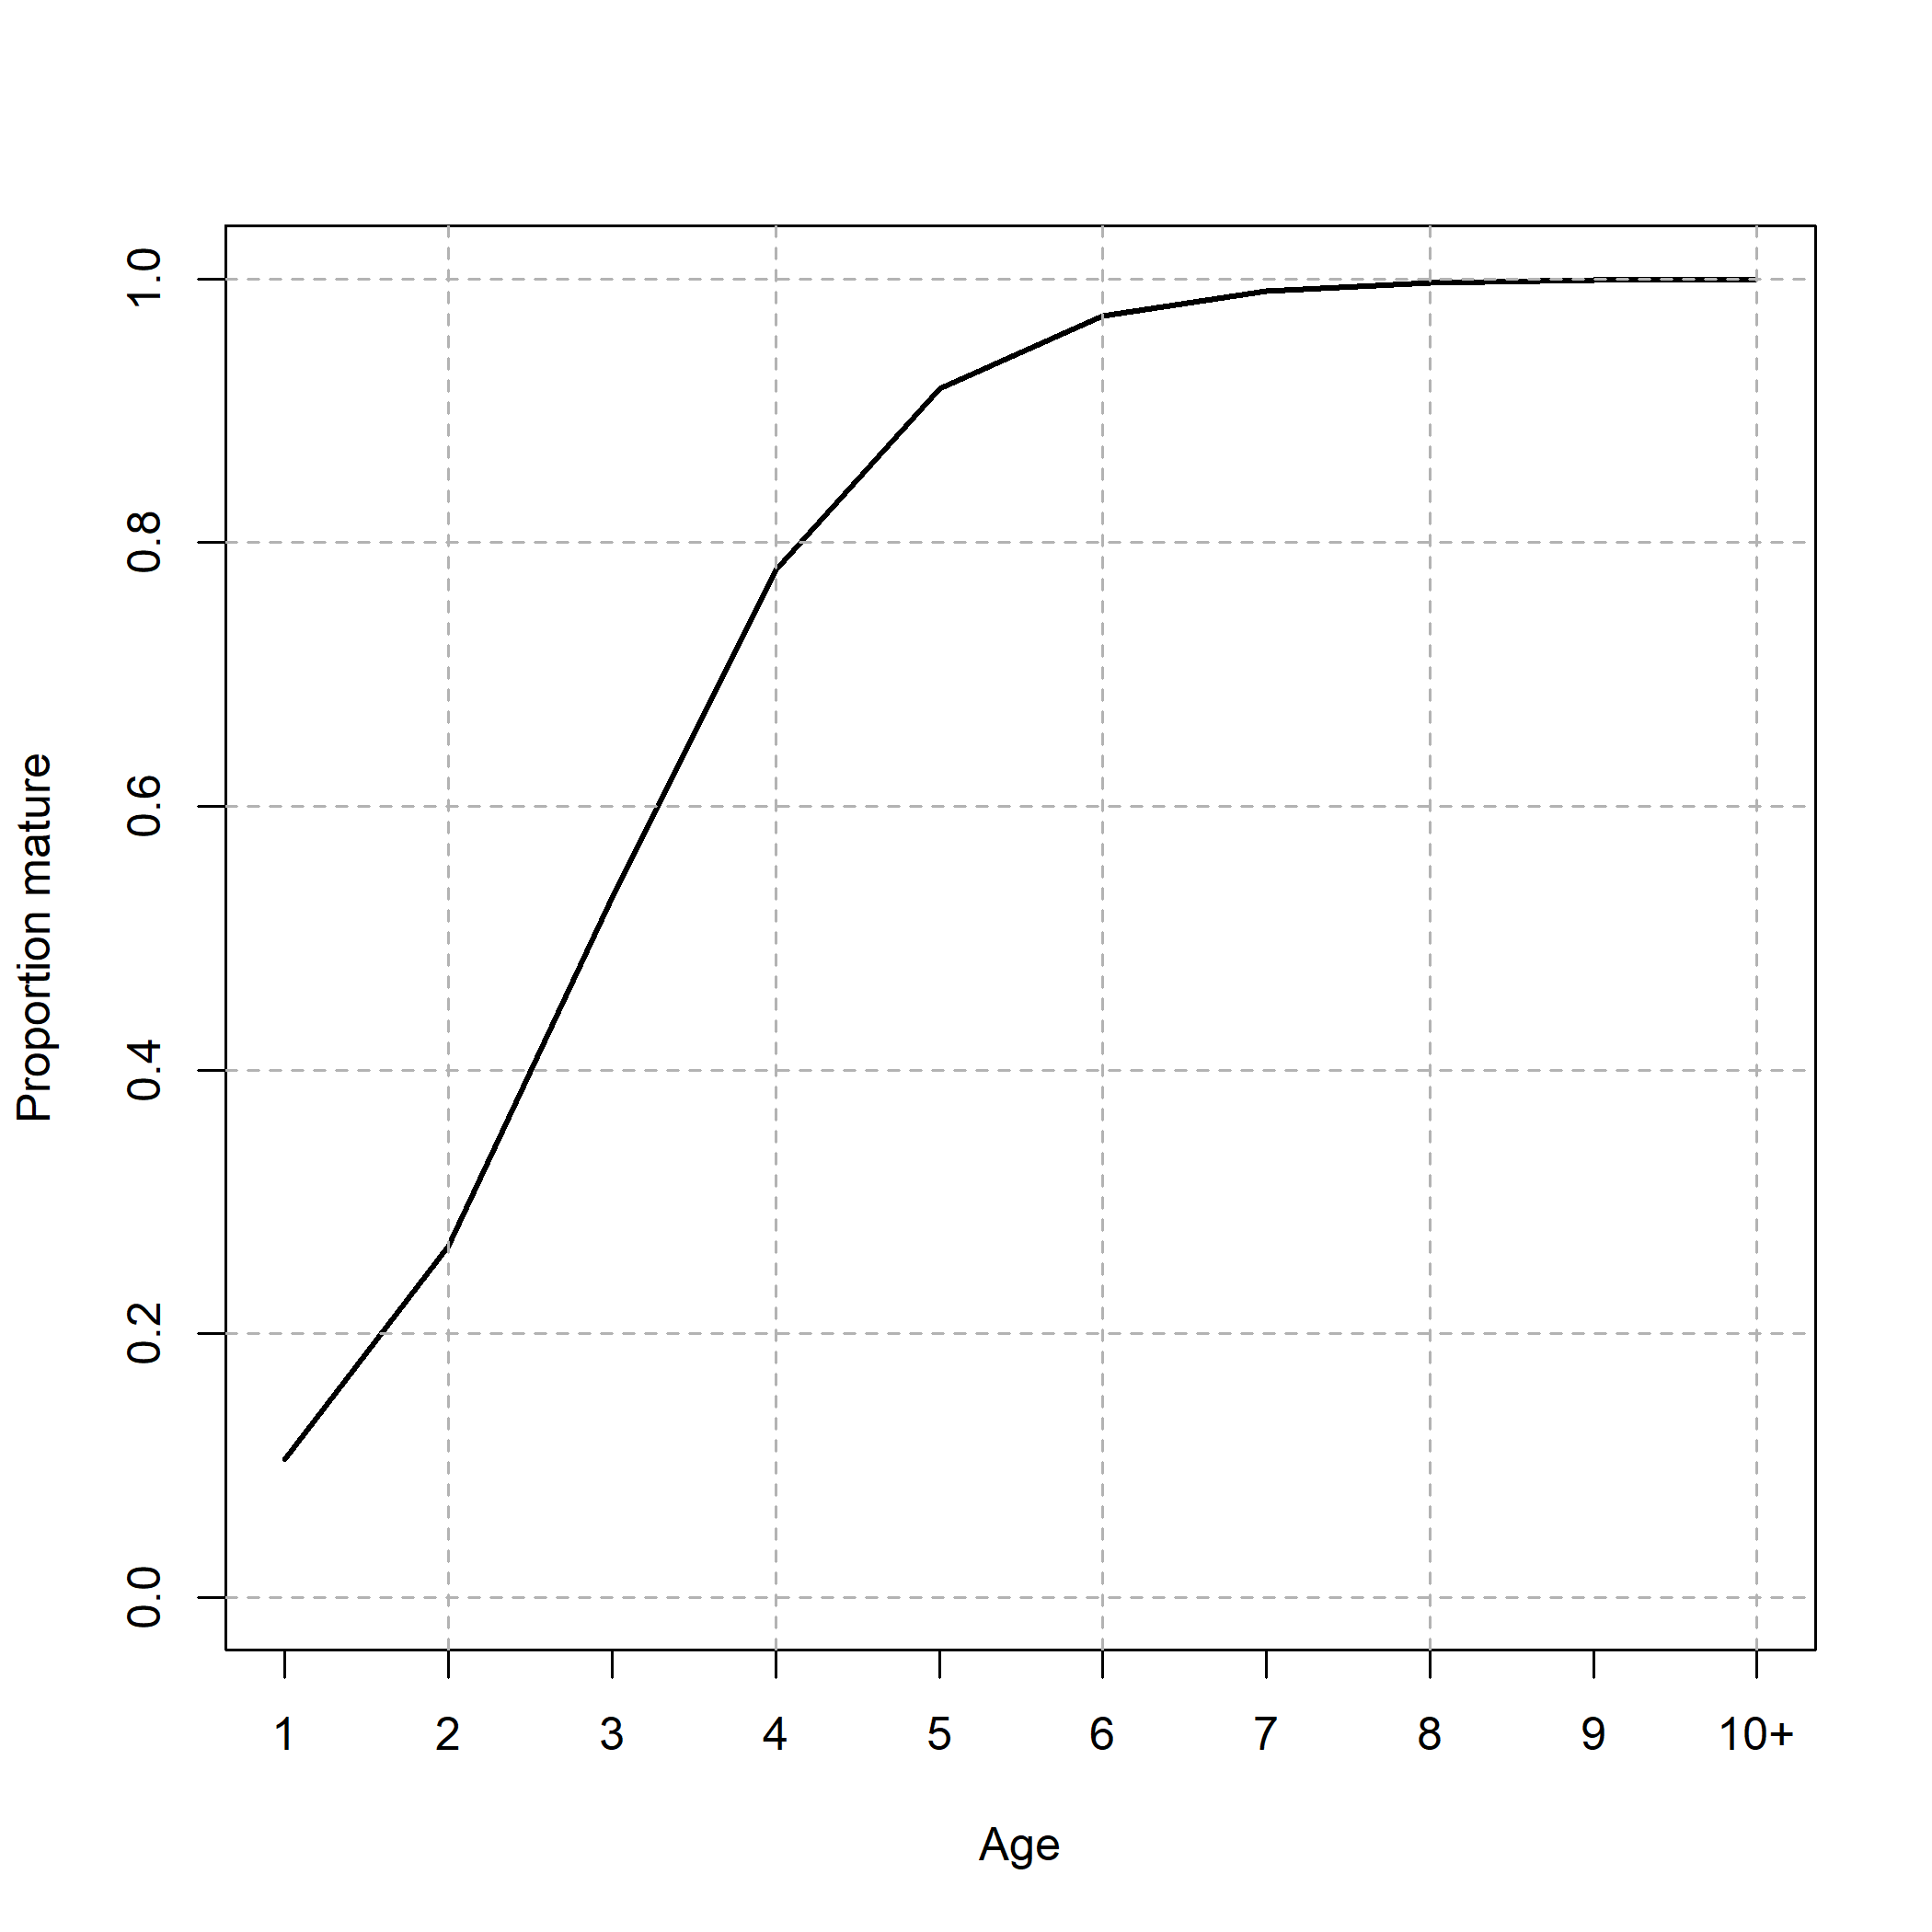
\includegraphics[width = \textwidth]{om_maturity.png}
\end{center}
\end{figure}

\begin{figure}
\caption{The weight at age assumed for the population in all operating and estimating models.}\label{om_waa}
\begin{center}
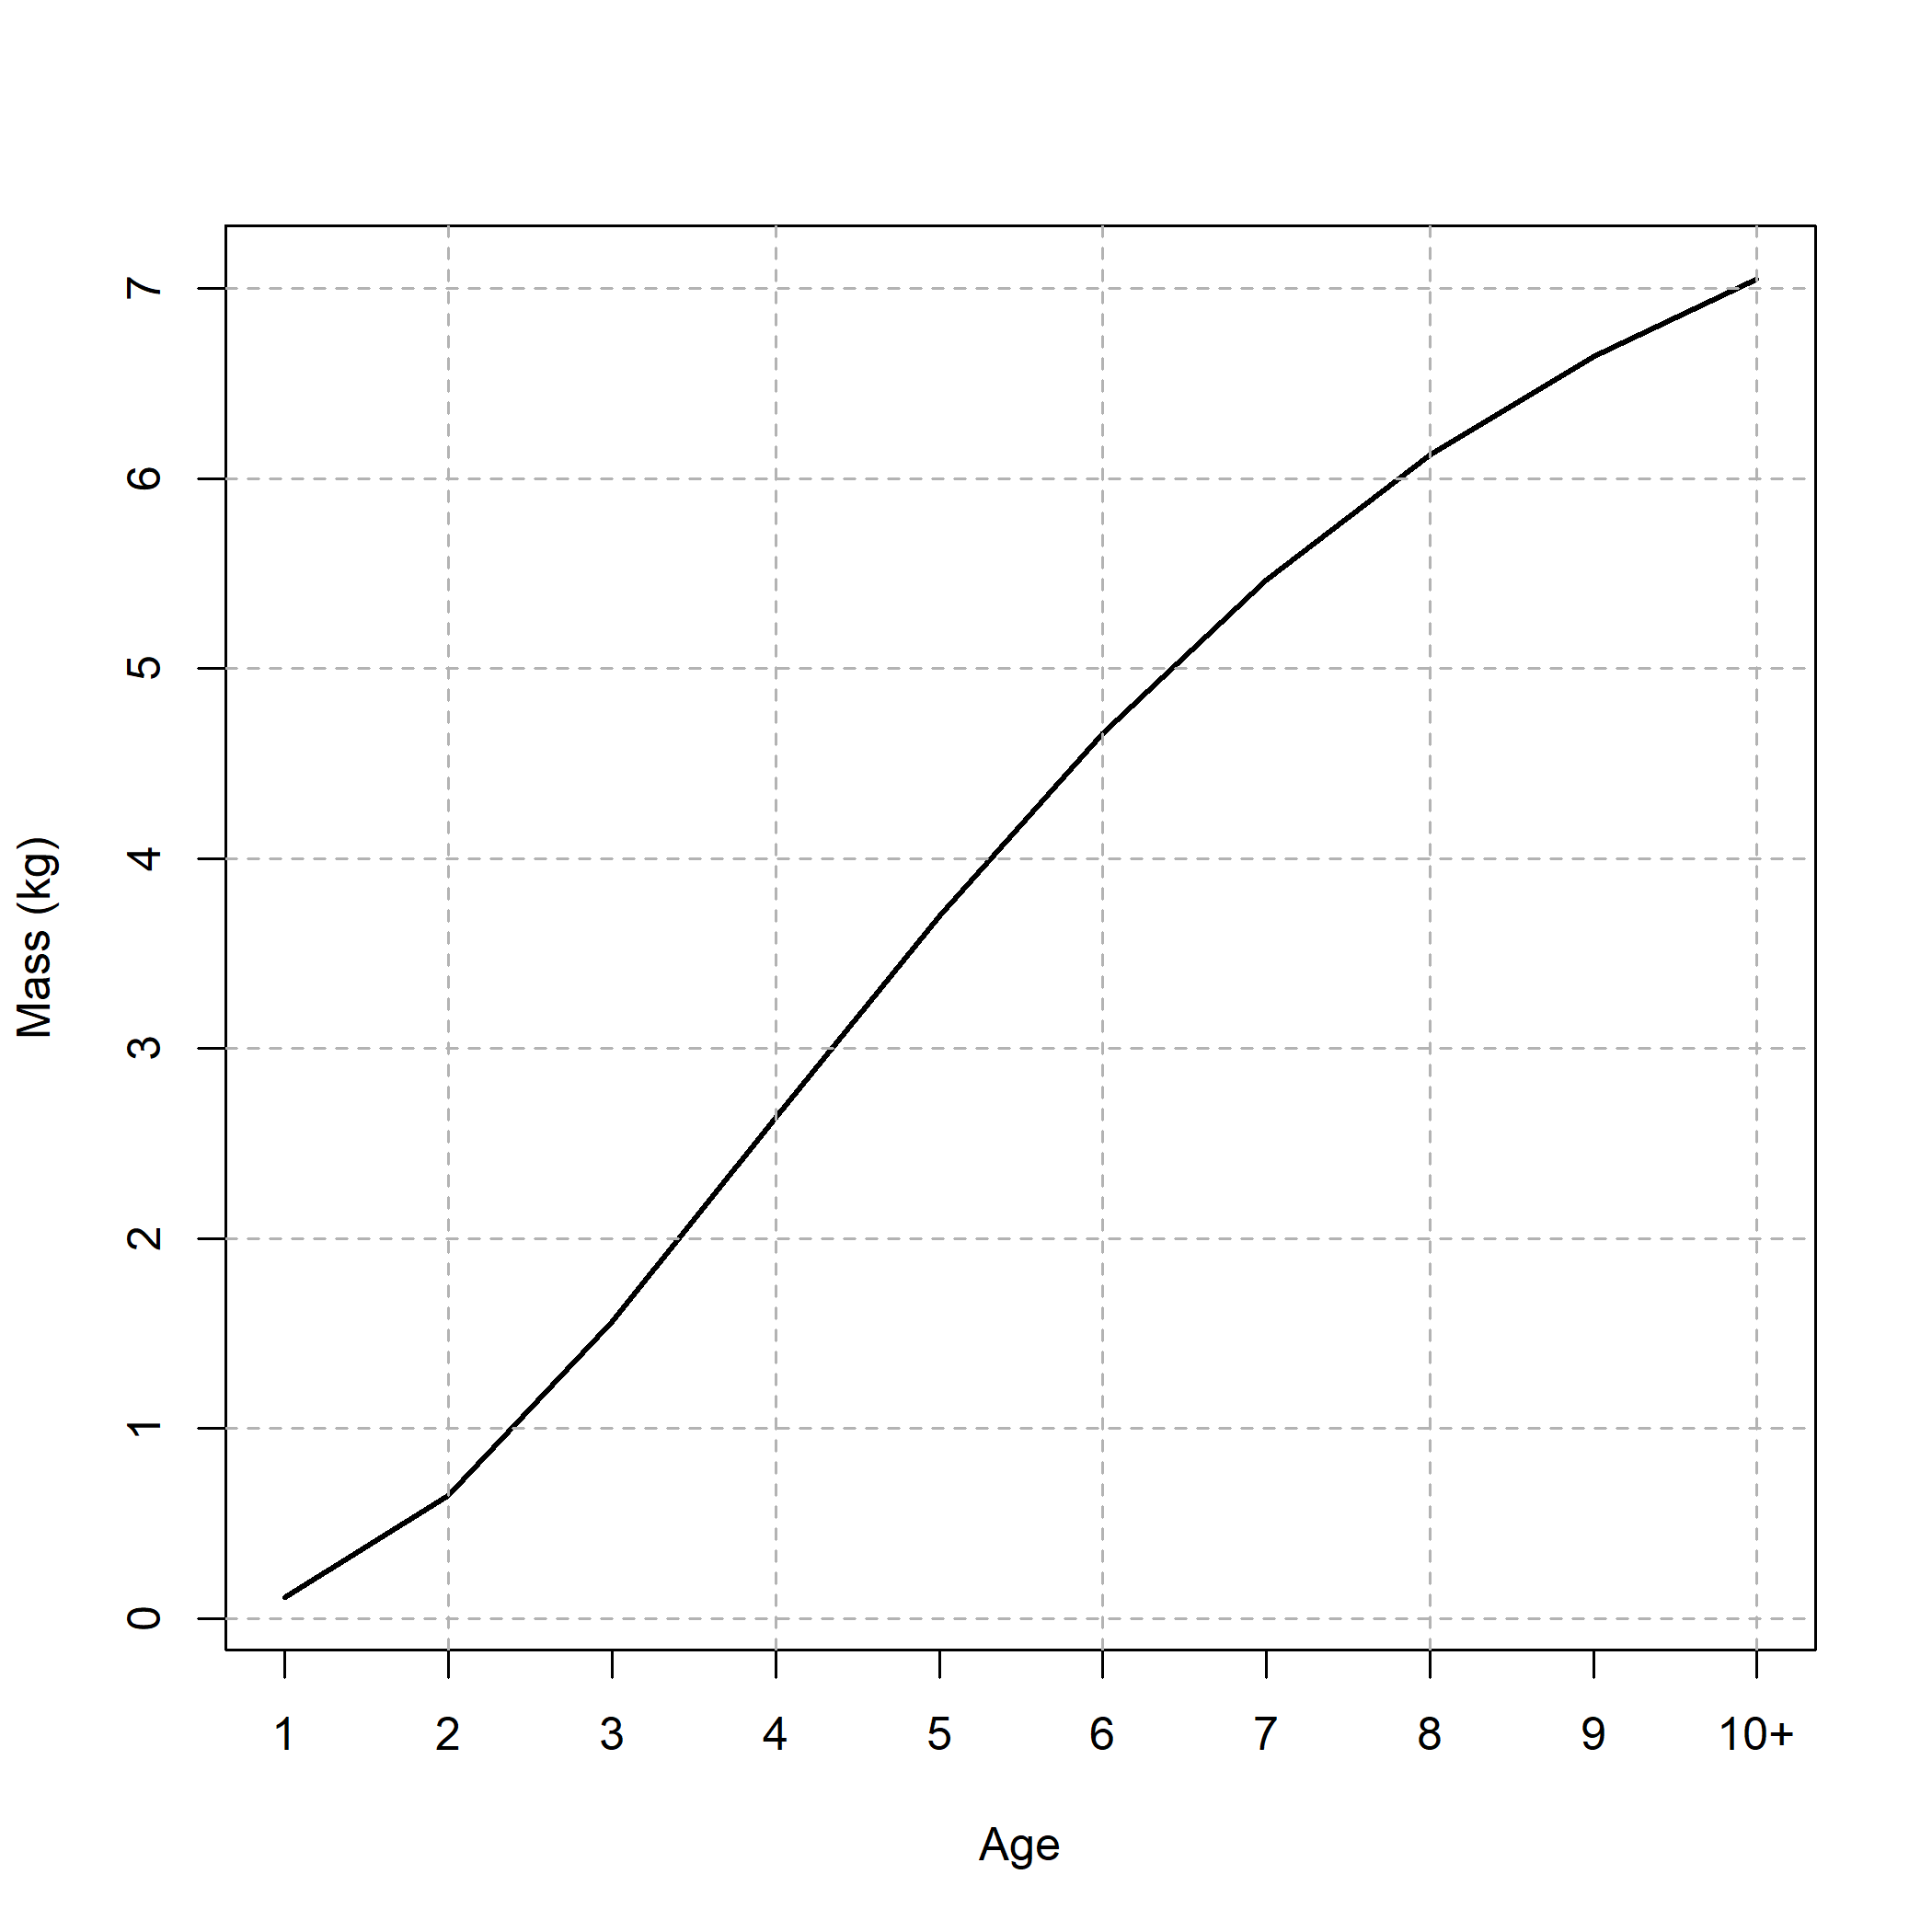
\includegraphics[width = \textwidth]{om_waa.png}
\end{center}
\end{figure}

\begin{figure}
\caption{The Beverton-Holt stock recruit relationship assume for all operating models.}\label{om_sr}
\begin{center}
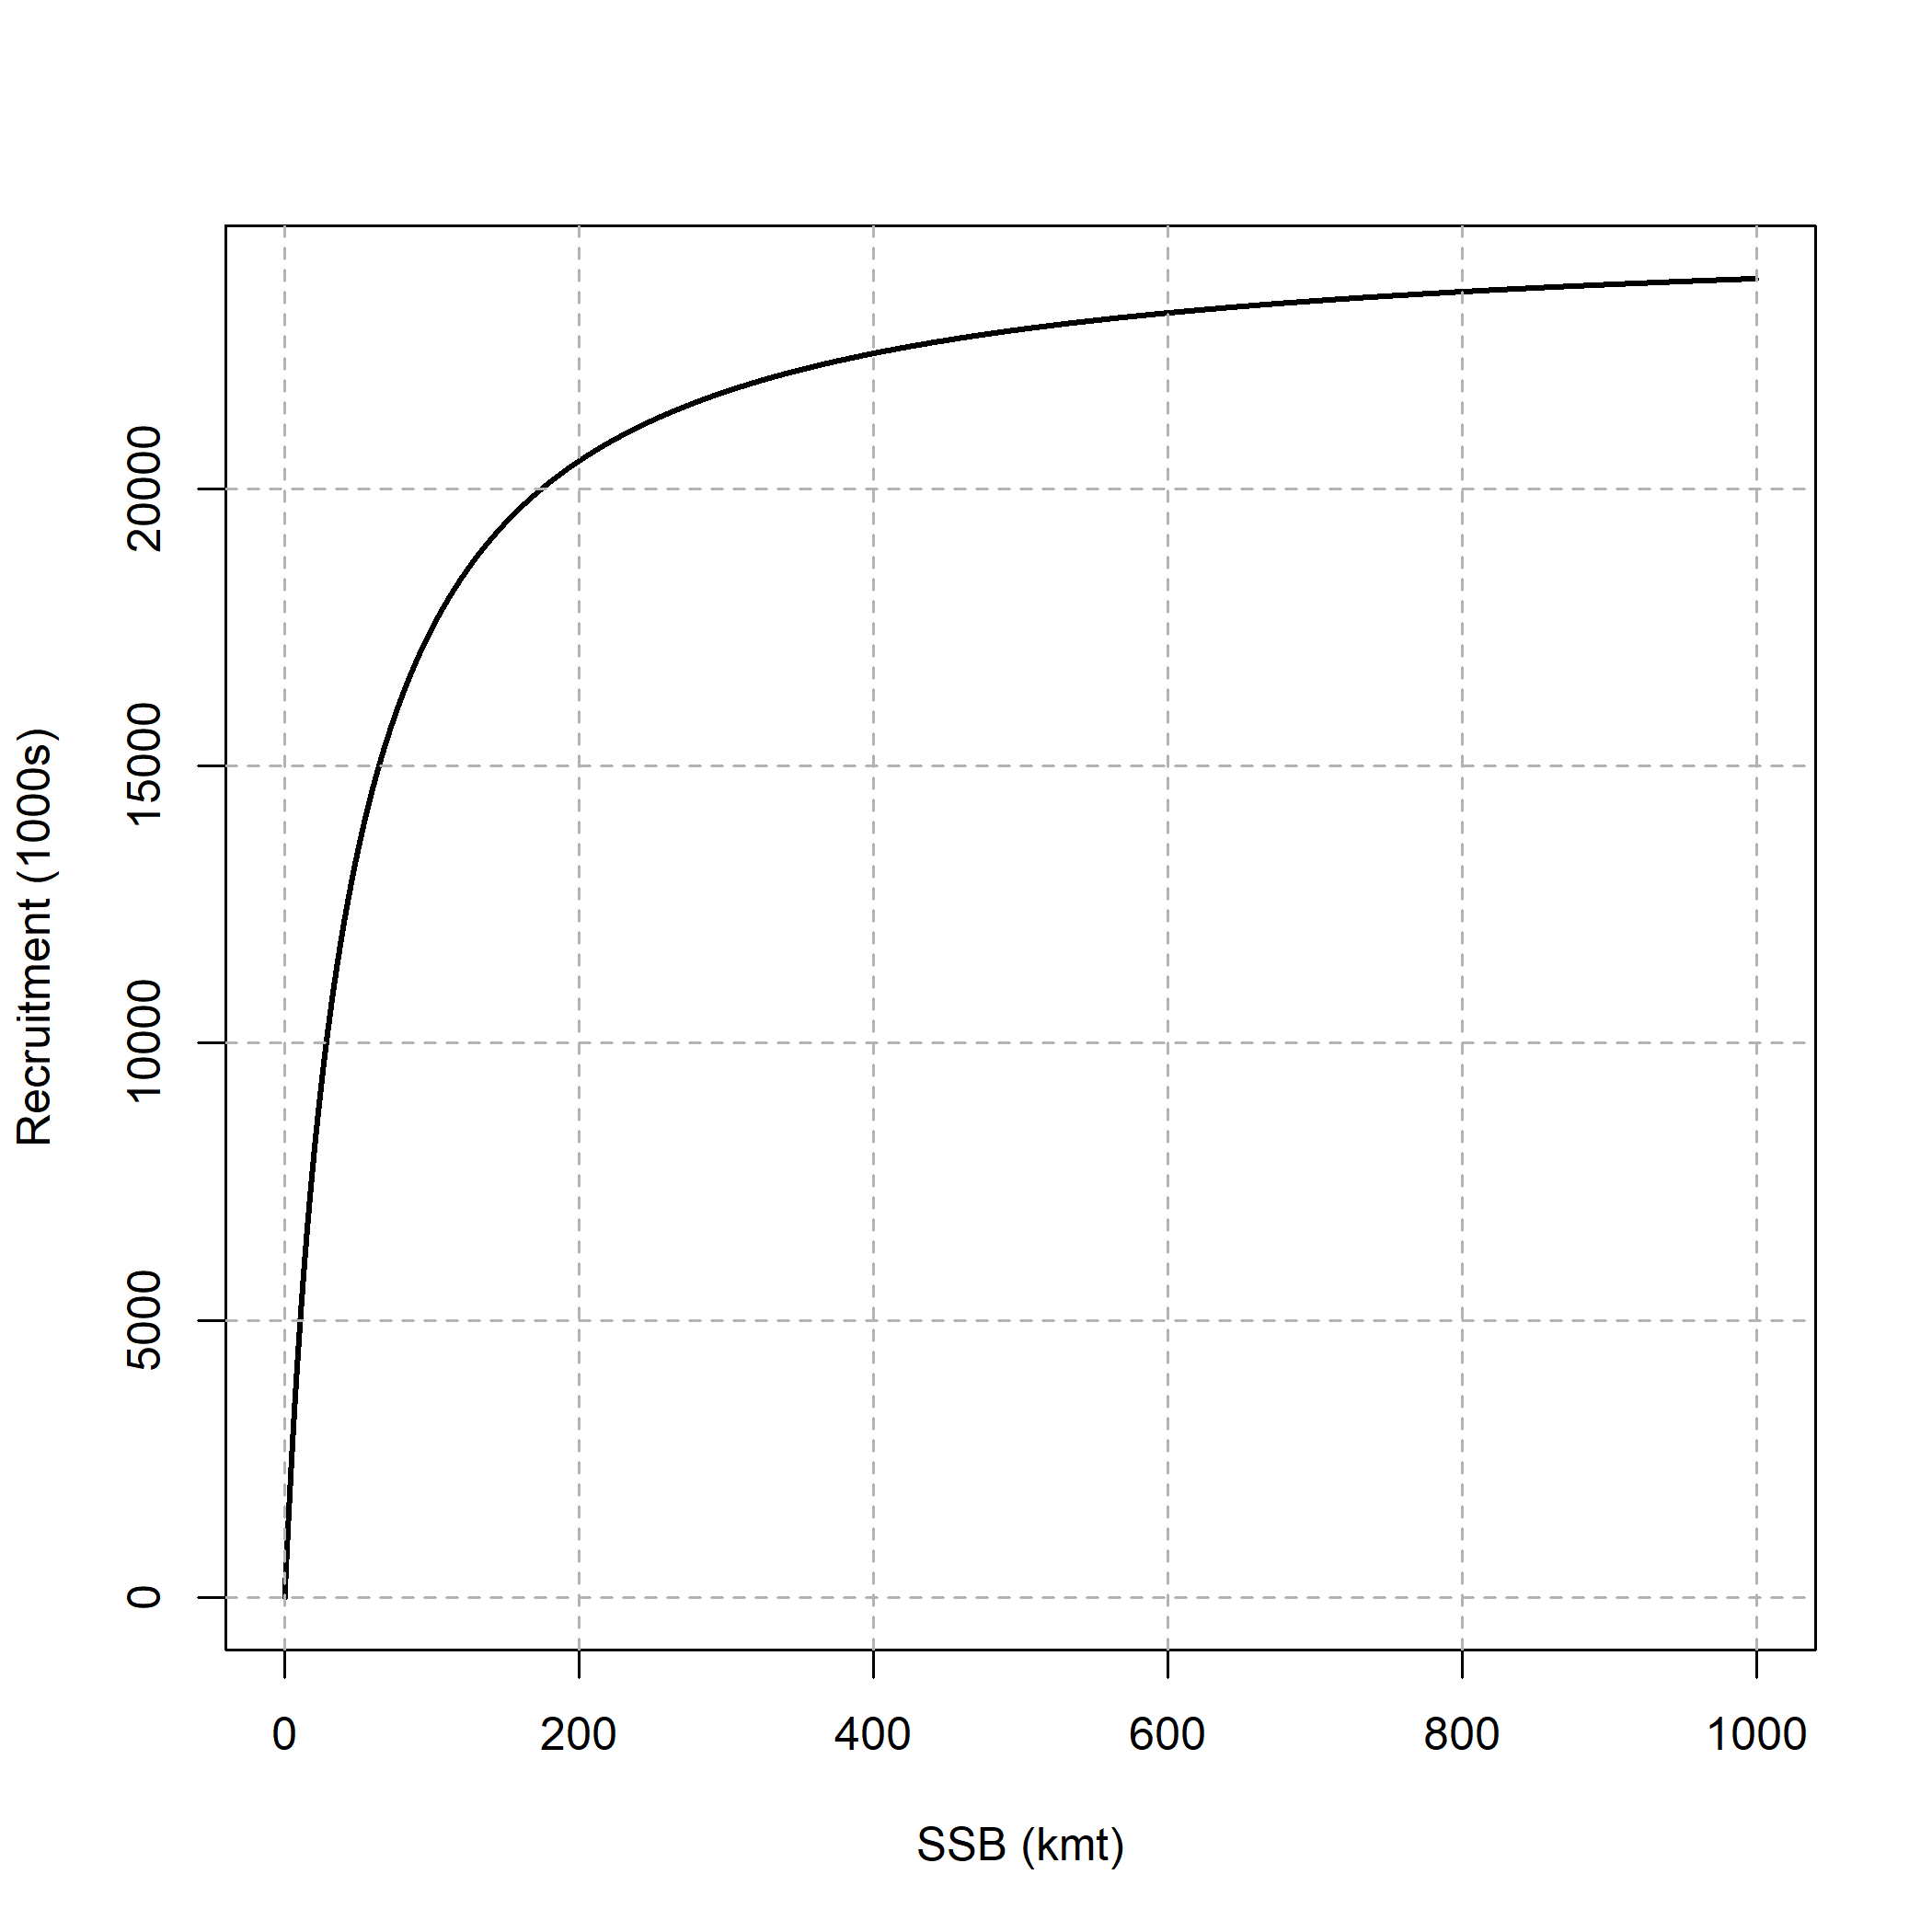
\includegraphics[width = \textwidth]{om_sr.png}
\end{center}
\end{figure}

\begin{figure}
\caption{The selectivity at age assumed for the fishing fleet in operating models without selectivity random effects. The mean selectivity at age across time for the fishing fleet in operating models with selectivity random effects.}\label{om_mean_selectivity}
\begin{center}
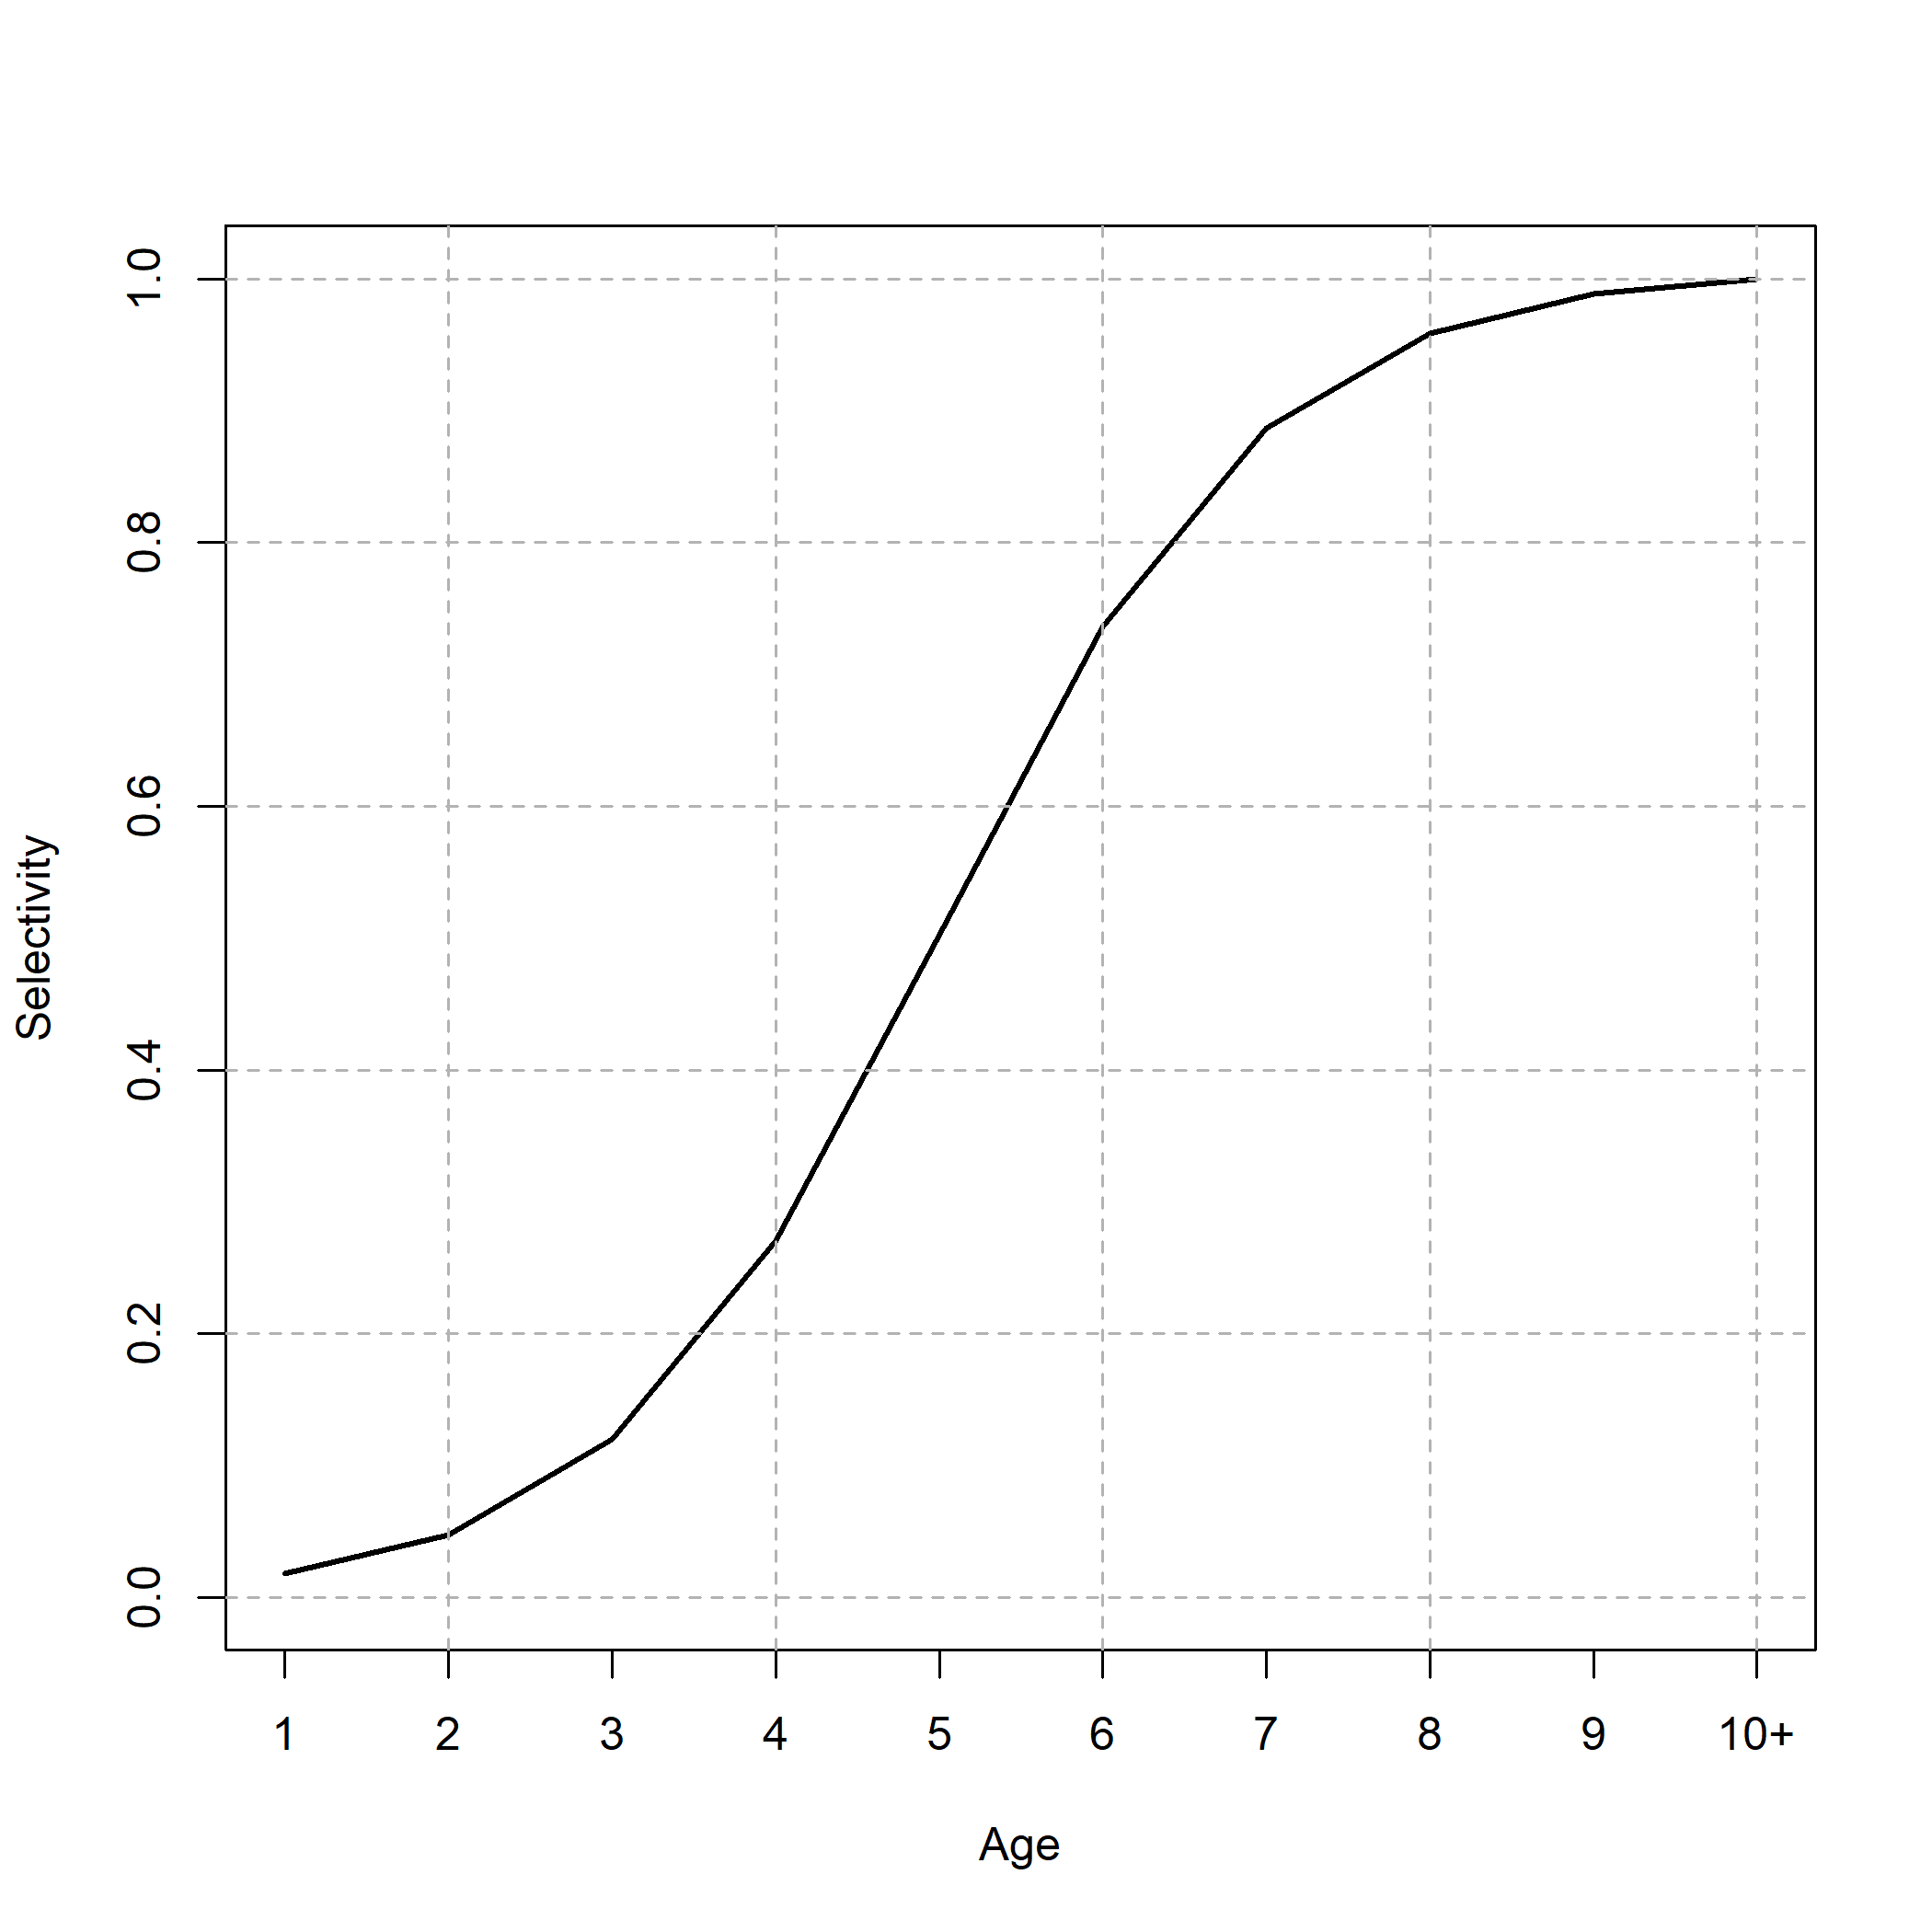
\includegraphics[width = \textwidth]{om_mean_selectivity.png}
\end{center}
\end{figure}

\begin{landscape}
\begin{figure}
\caption{Probability of each type of convergence of estimating models with alternative process error assumptions for operating models that have process error structures R and R+S. vertical lines represent 95\% confidence intervals. All estimating models estimate mean recruitment rather than a stock-recruit relationship and and M is fixed at the true value.}\label{naa_om_em_R_MF_convergence}
\begin{center}
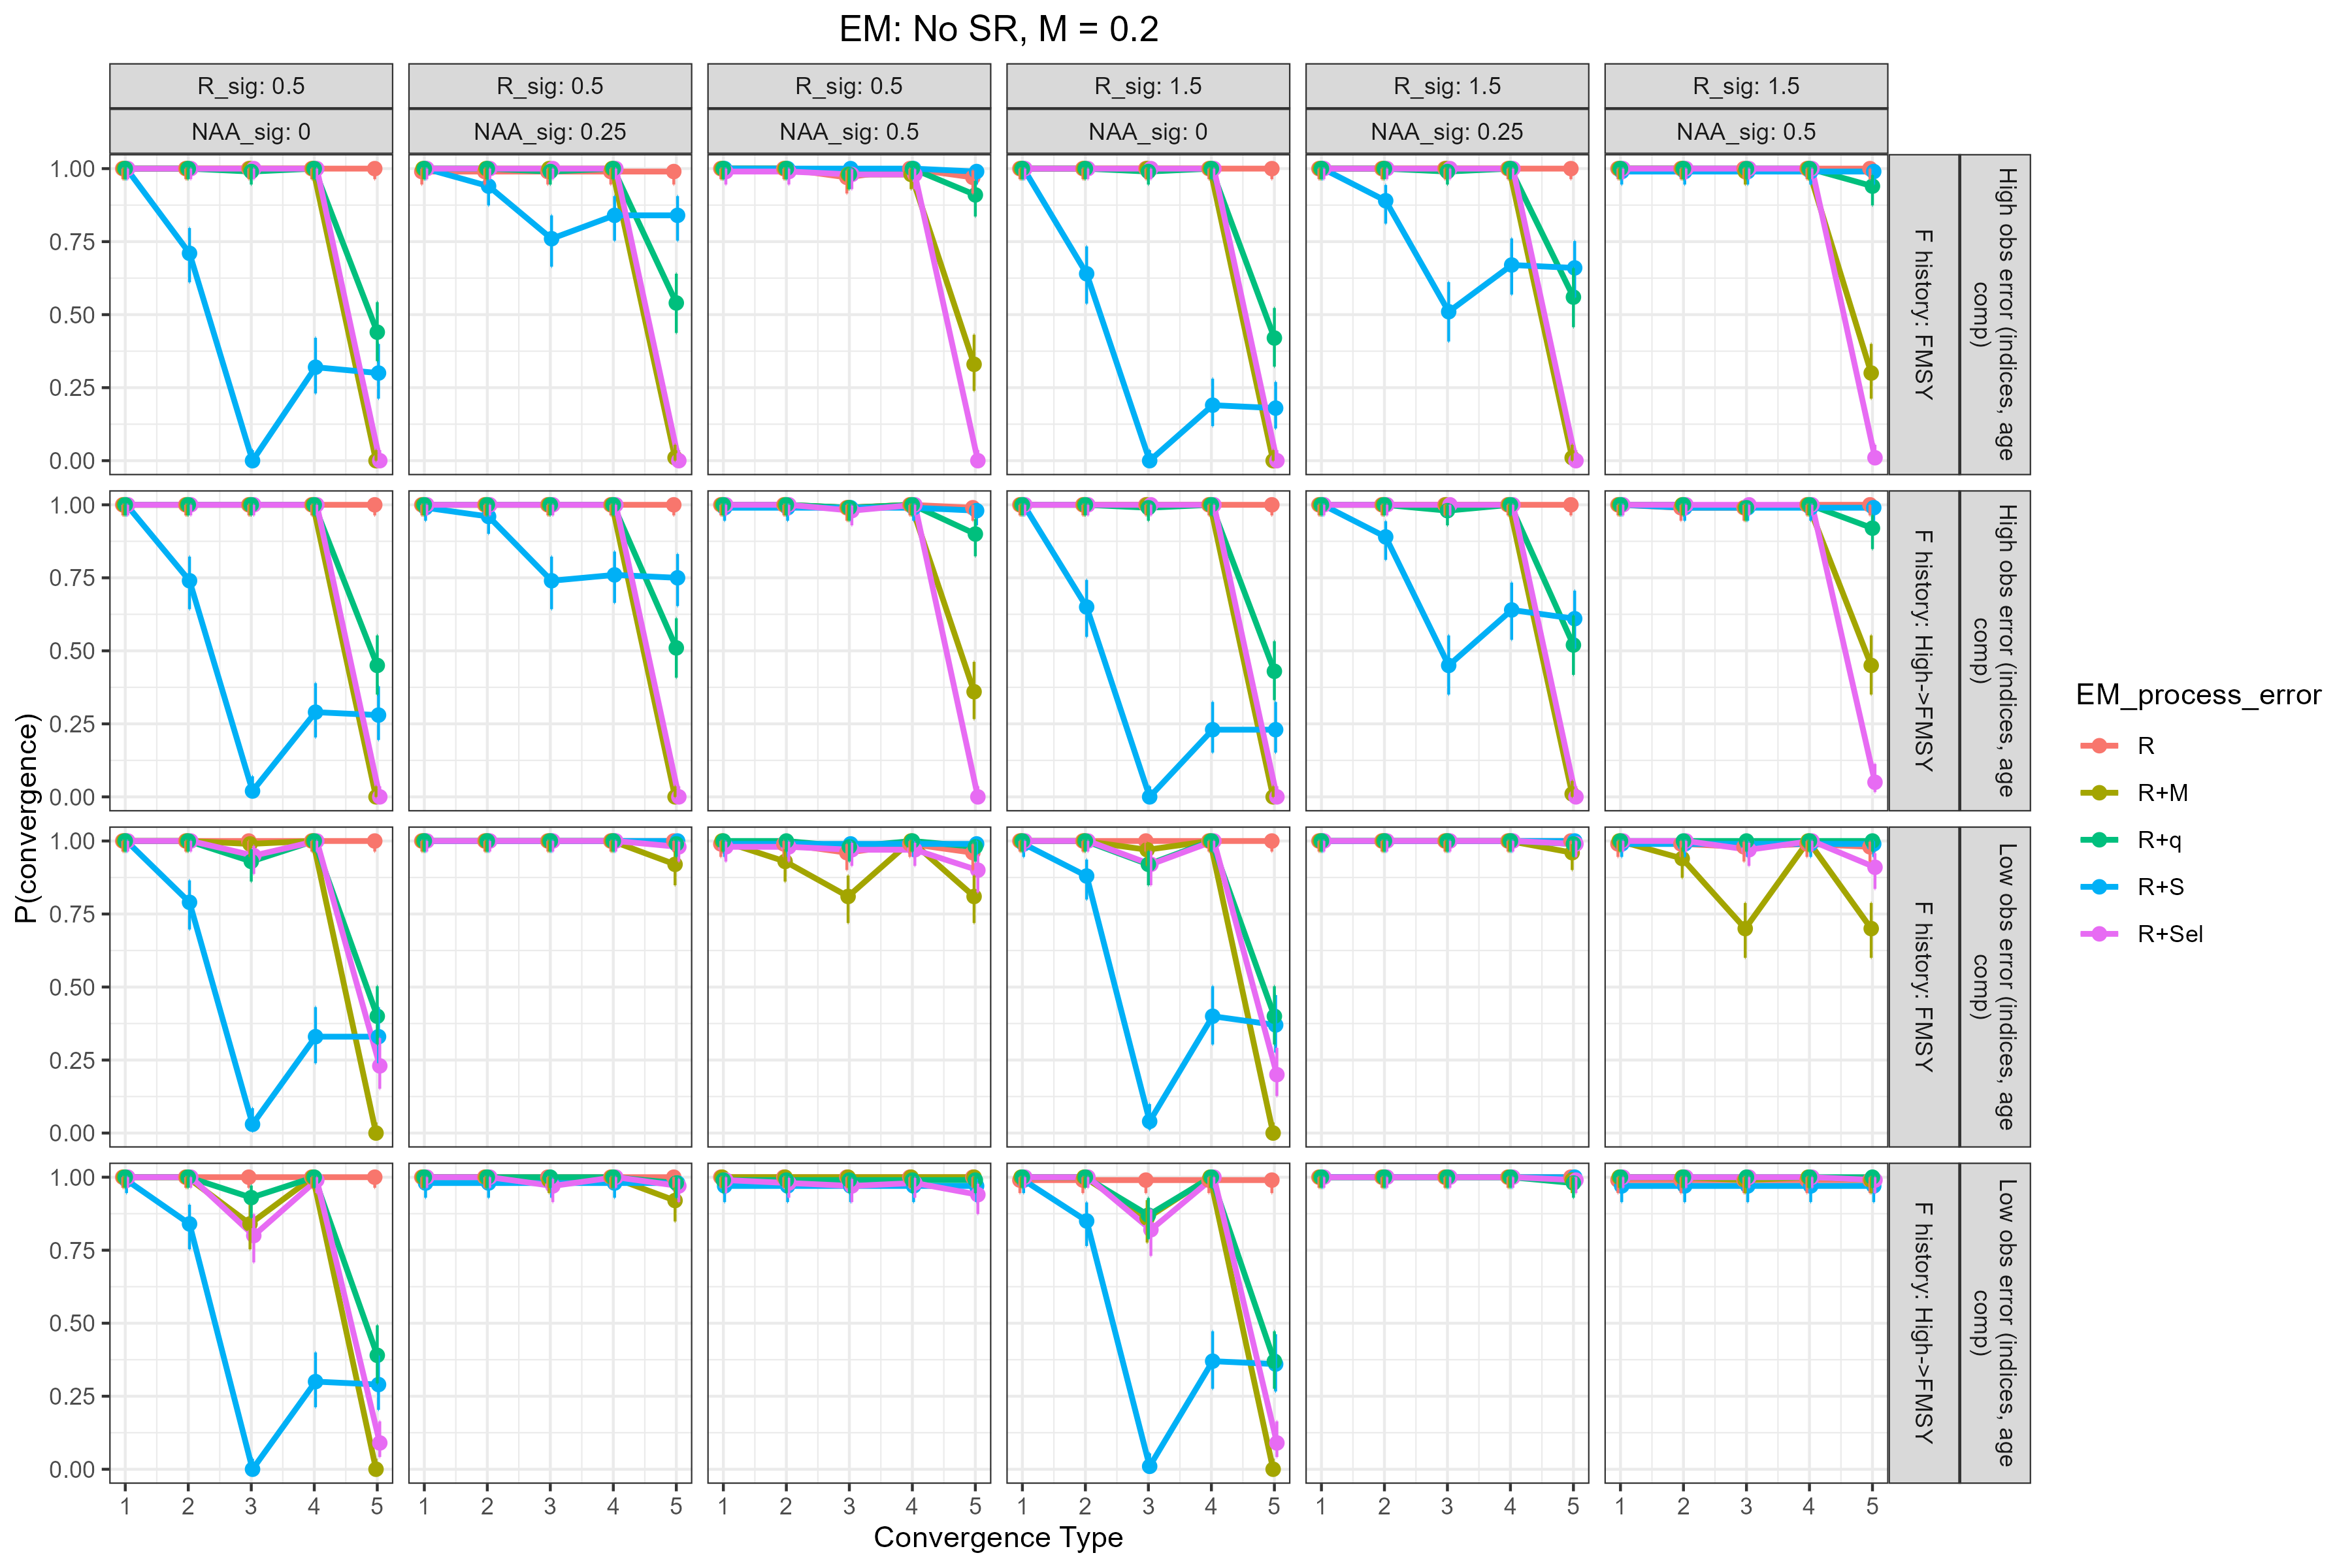
\includegraphics[width = \textwidth]{naa_om_p_convergence_meanR_M_fixed.png}
\end{center}
\end{figure}
\end{landscape}

\begin{landscape}
\begin{figure}
\caption{Probability of each type of convergence of estimating models with alternative process error assumptions for operating models that have process error structures R and R+S. vertical lines represent 95\% confidence intervals. All estimating models estimate mean recruitment rather than a stock-recruit relationship and and M is estimated.}\label{naa_om_em_R_ME_convergence}
\begin{center}
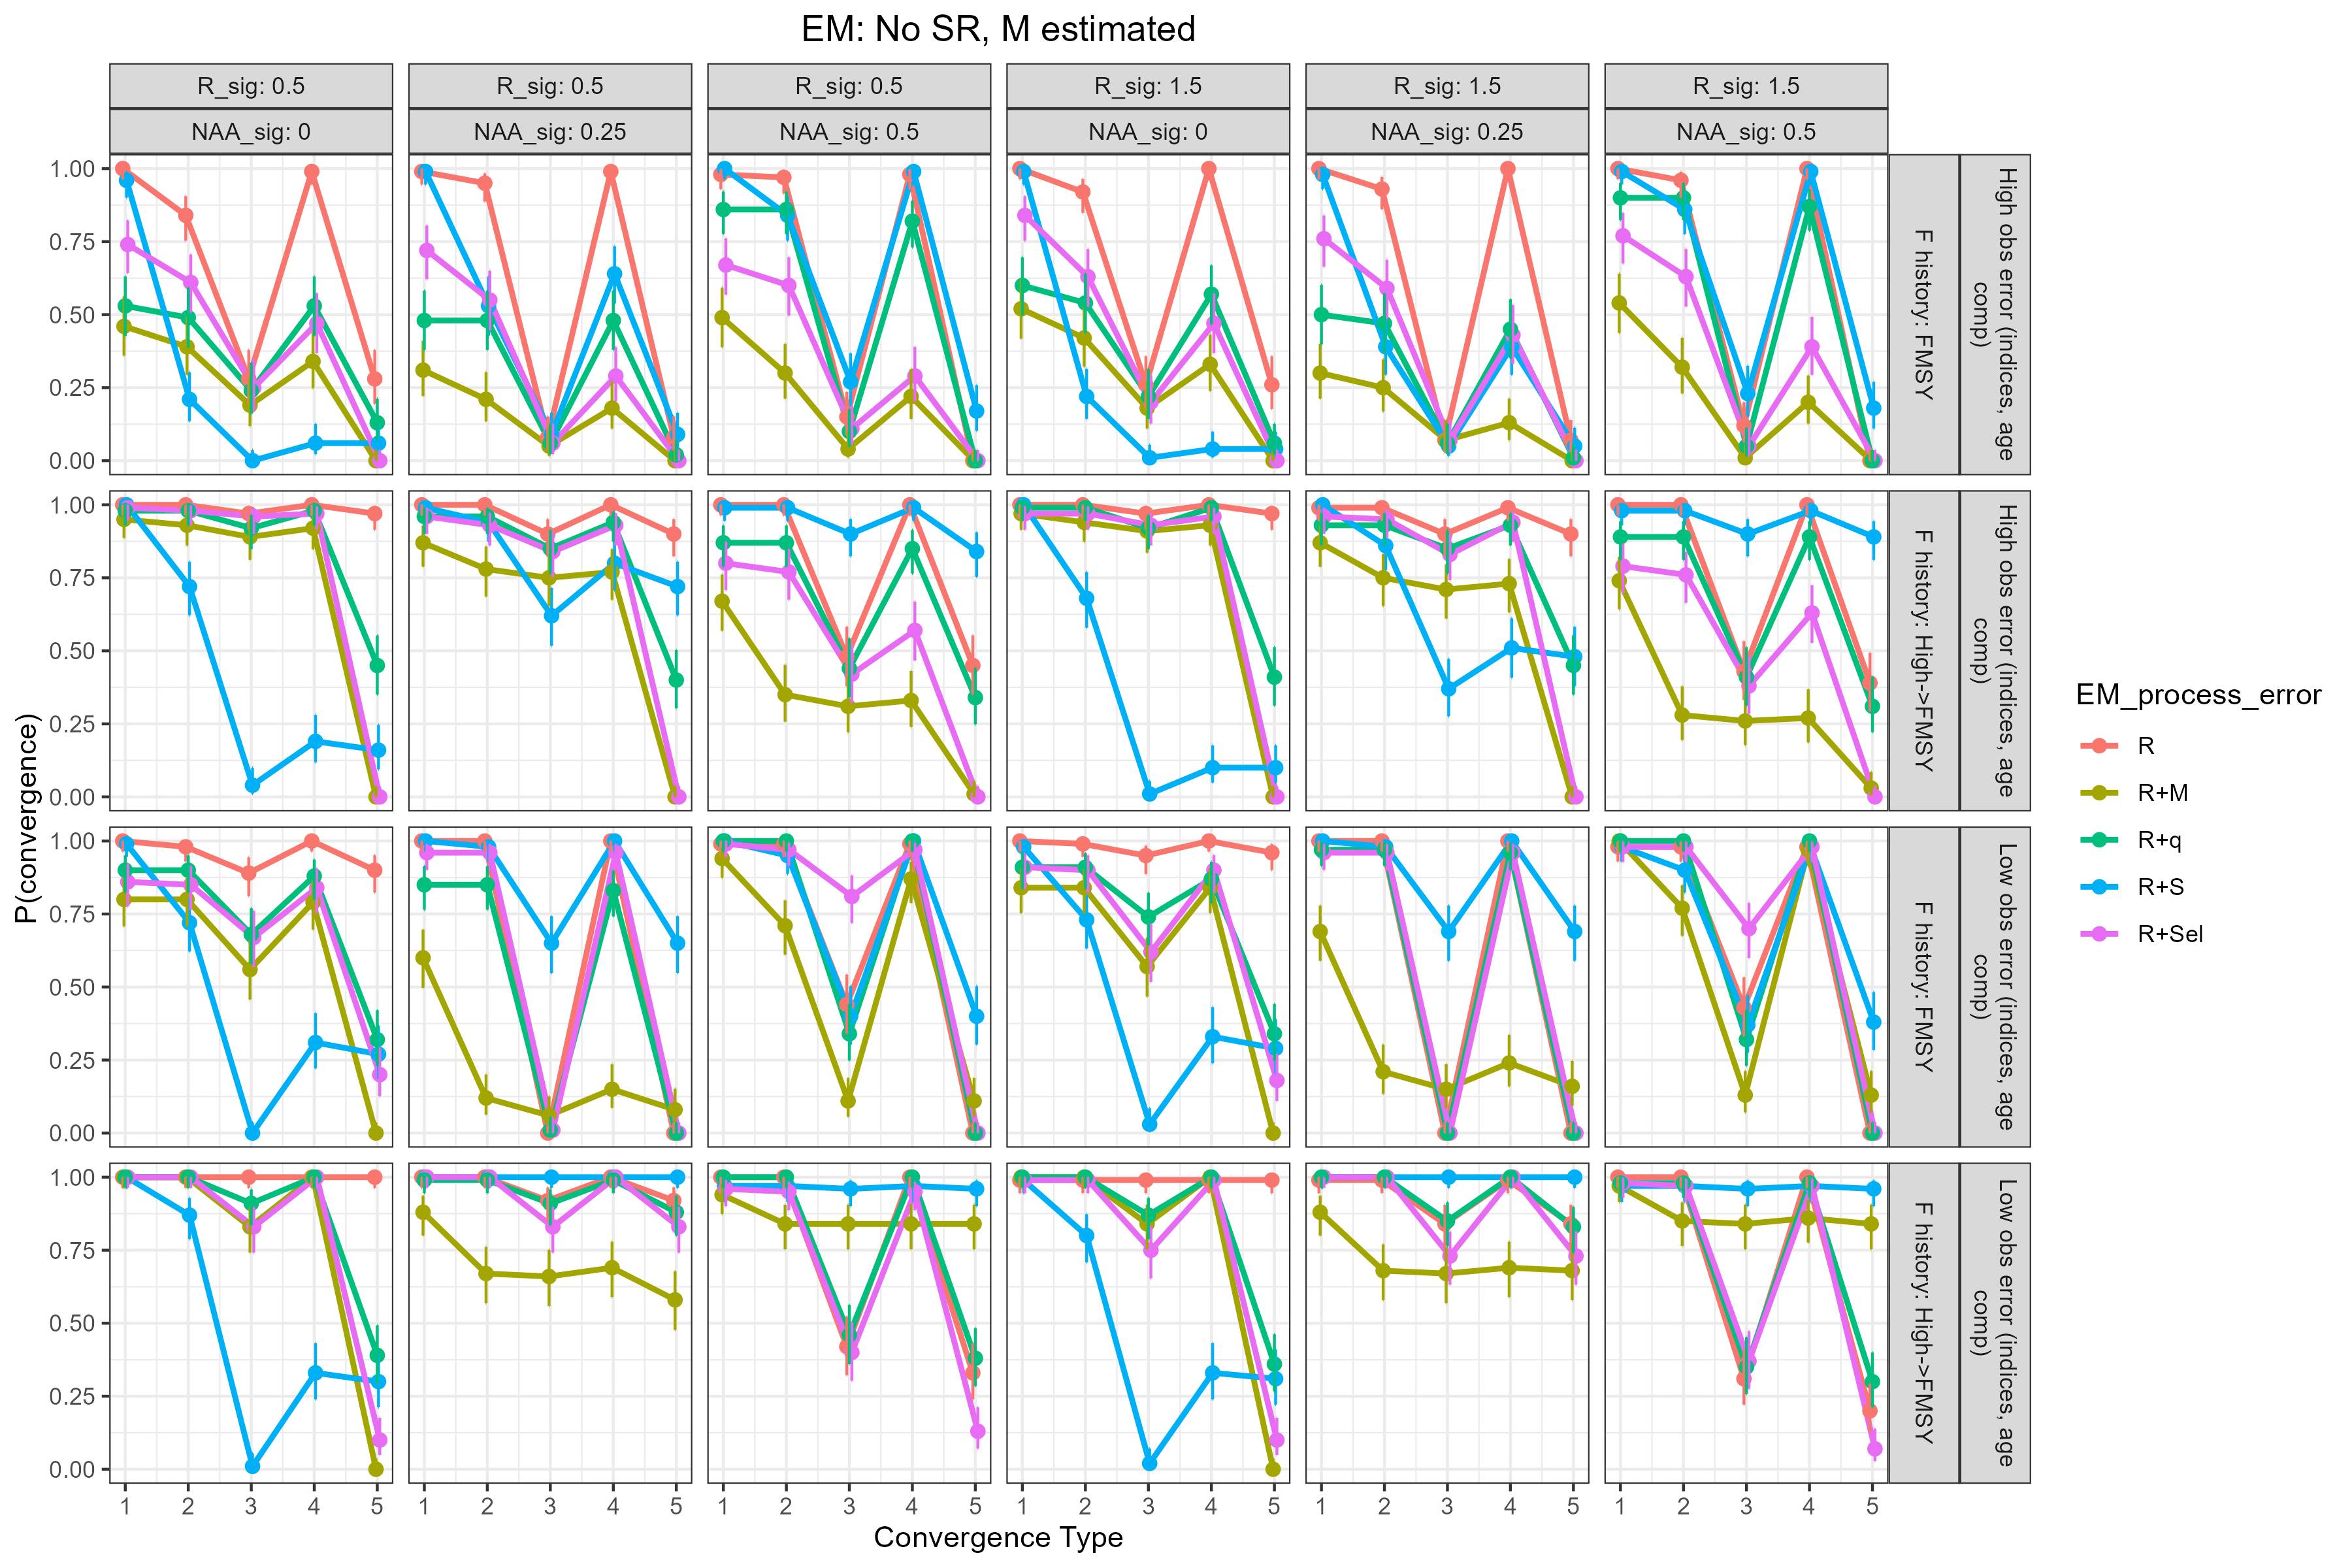
\includegraphics[width = \textwidth]{naa_om_p_convergence_meanR_M_estimated.png}
\end{center}
\end{figure}
\end{landscape}

\begin{landscape}
\begin{figure}
\caption{Probability of each type of convergence of estimating models with alternative process error assumptions for operating models that have process error structures R and R+S. vertical lines represent 95\% confidence intervals. All estimating models estimate a Beverton-Holt stock-recruit relationship and and M is fixed at the true value.}\label{naa_om_em_BH_MF_convergence}
\begin{center}
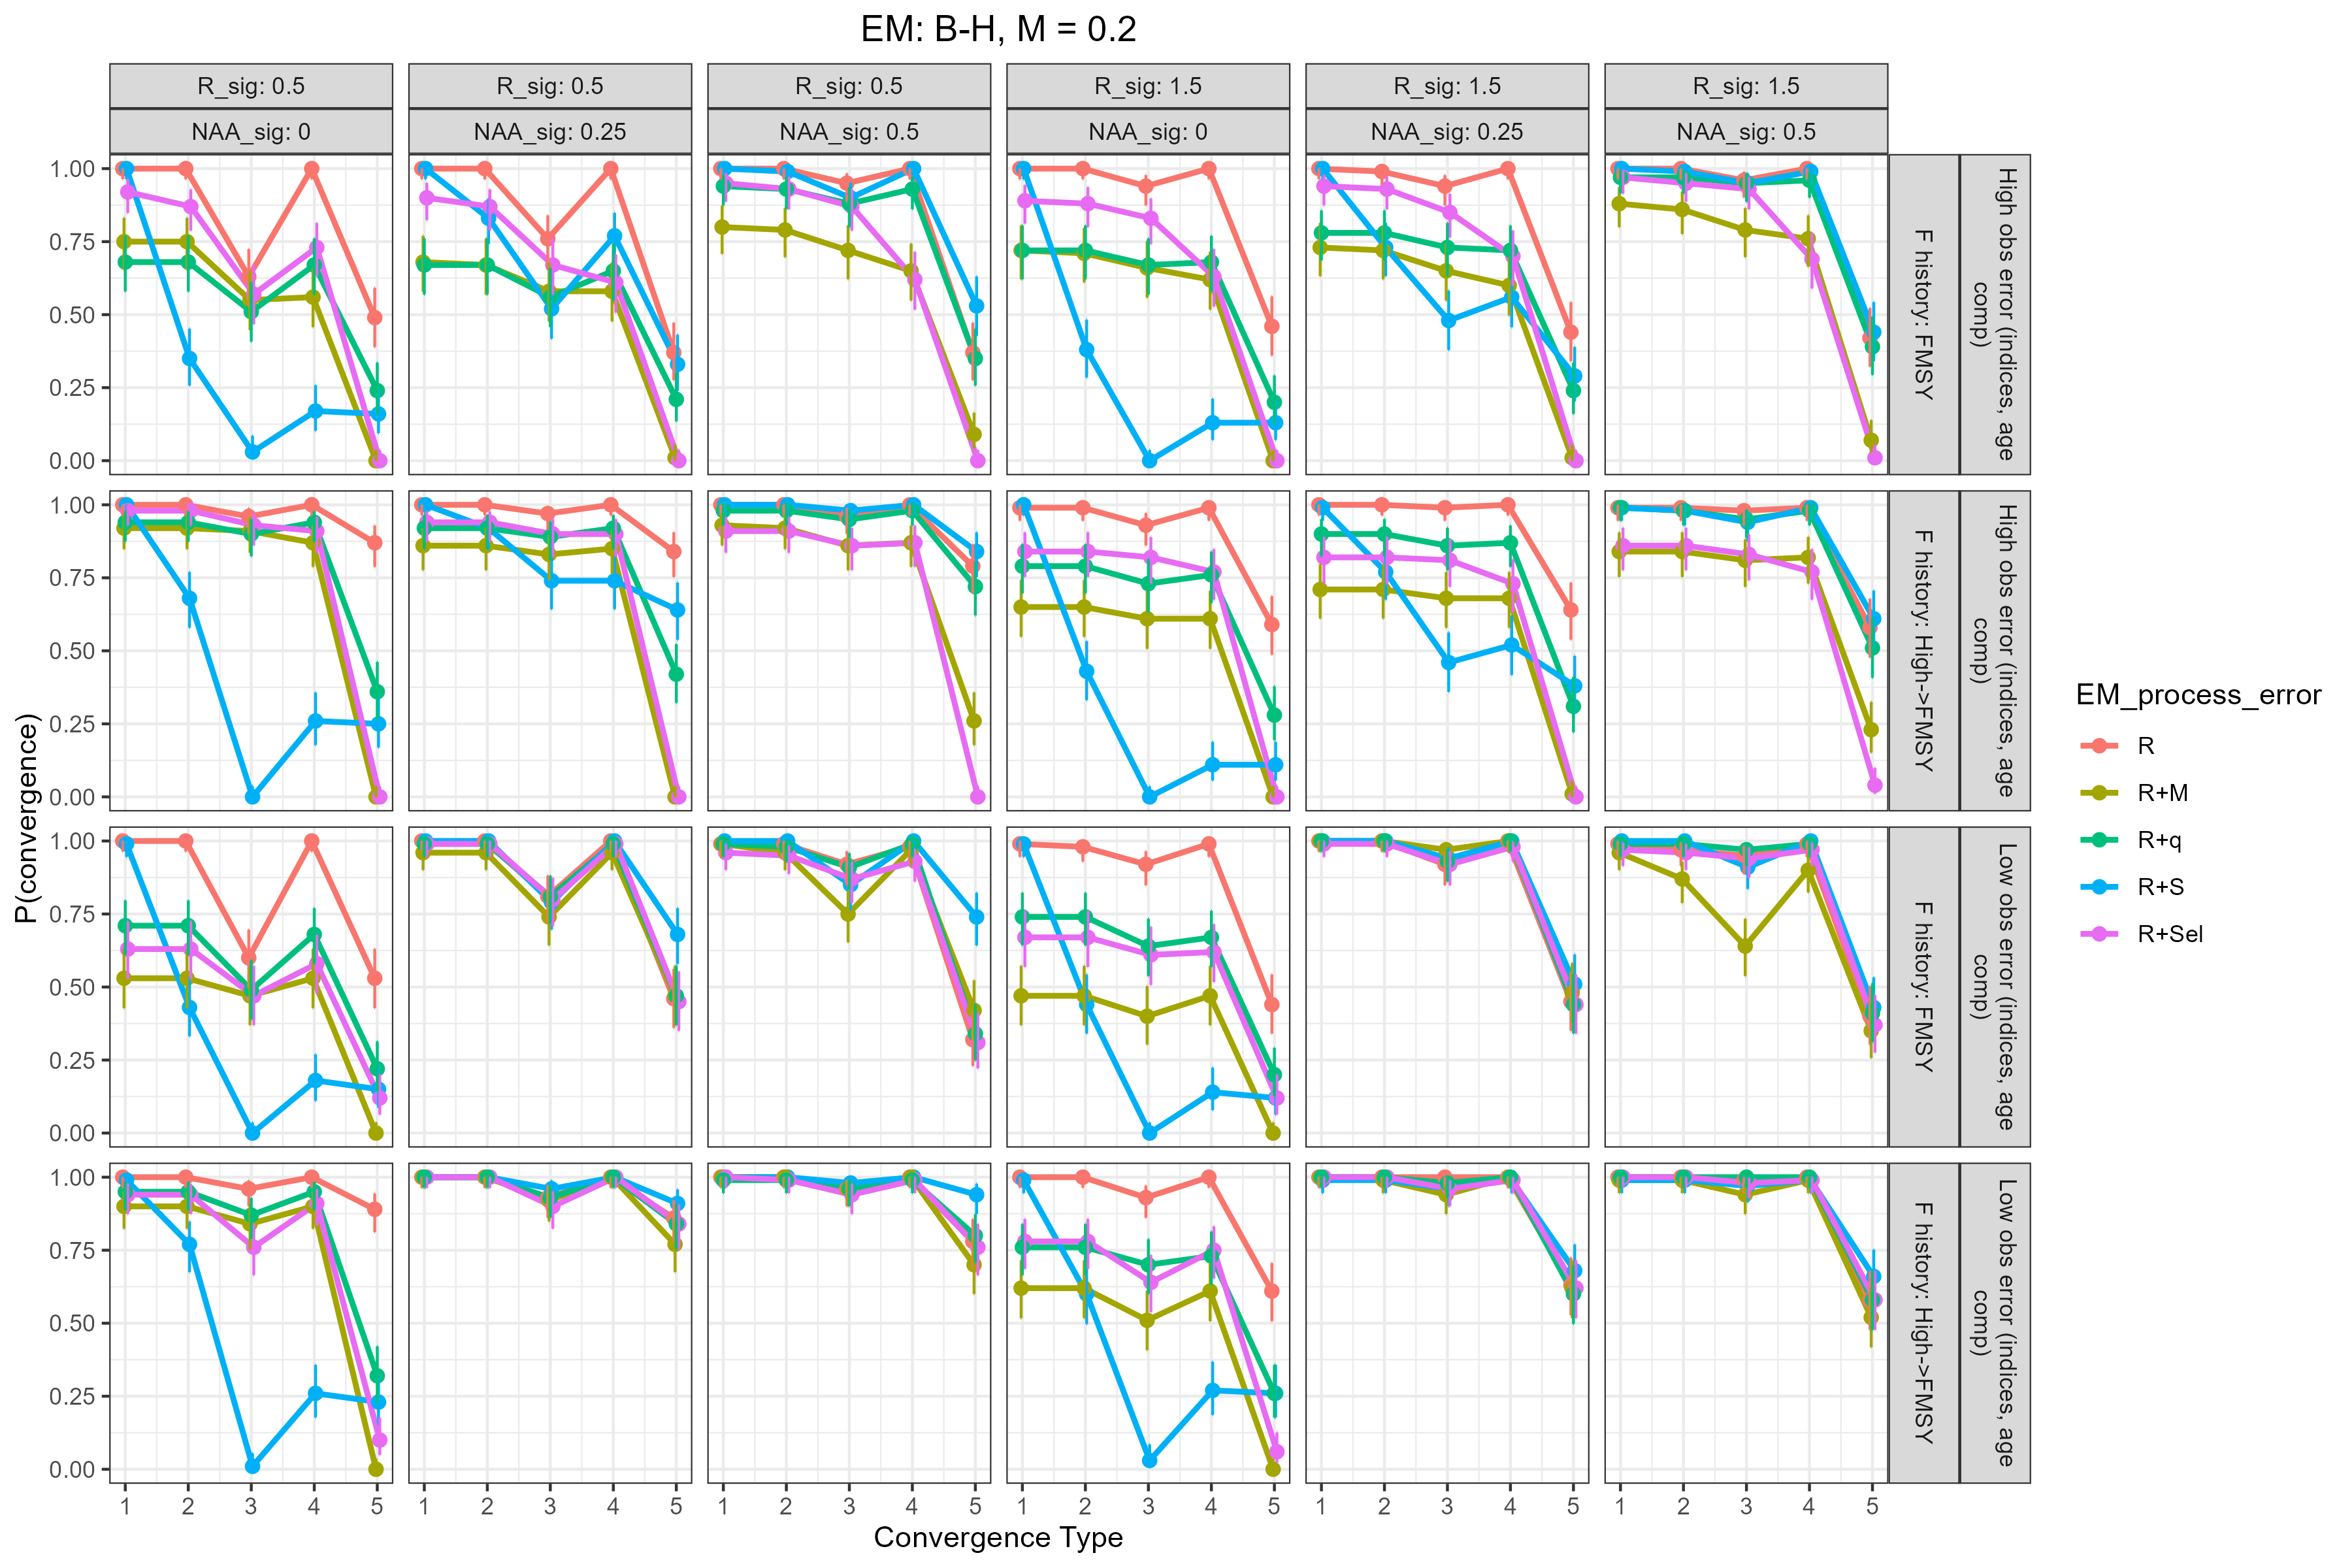
\includegraphics[width = \textwidth]{naa_om_p_convergence_BH_M_fixed.png}
\end{center}
\end{figure}
\end{landscape}

\begin{landscape}
\begin{figure}
\caption{Probability of each type of convergence of estimating models with alternative process error assumptions for operating models that have process error structures R and R+S. vertical lines represent 95\% confidence intervals. All estimating models estimate a Beverton-Holt stock-recruit relationship and and M is estimated.}\label{naa_om_em_BH_ME_convergence}
\begin{center}
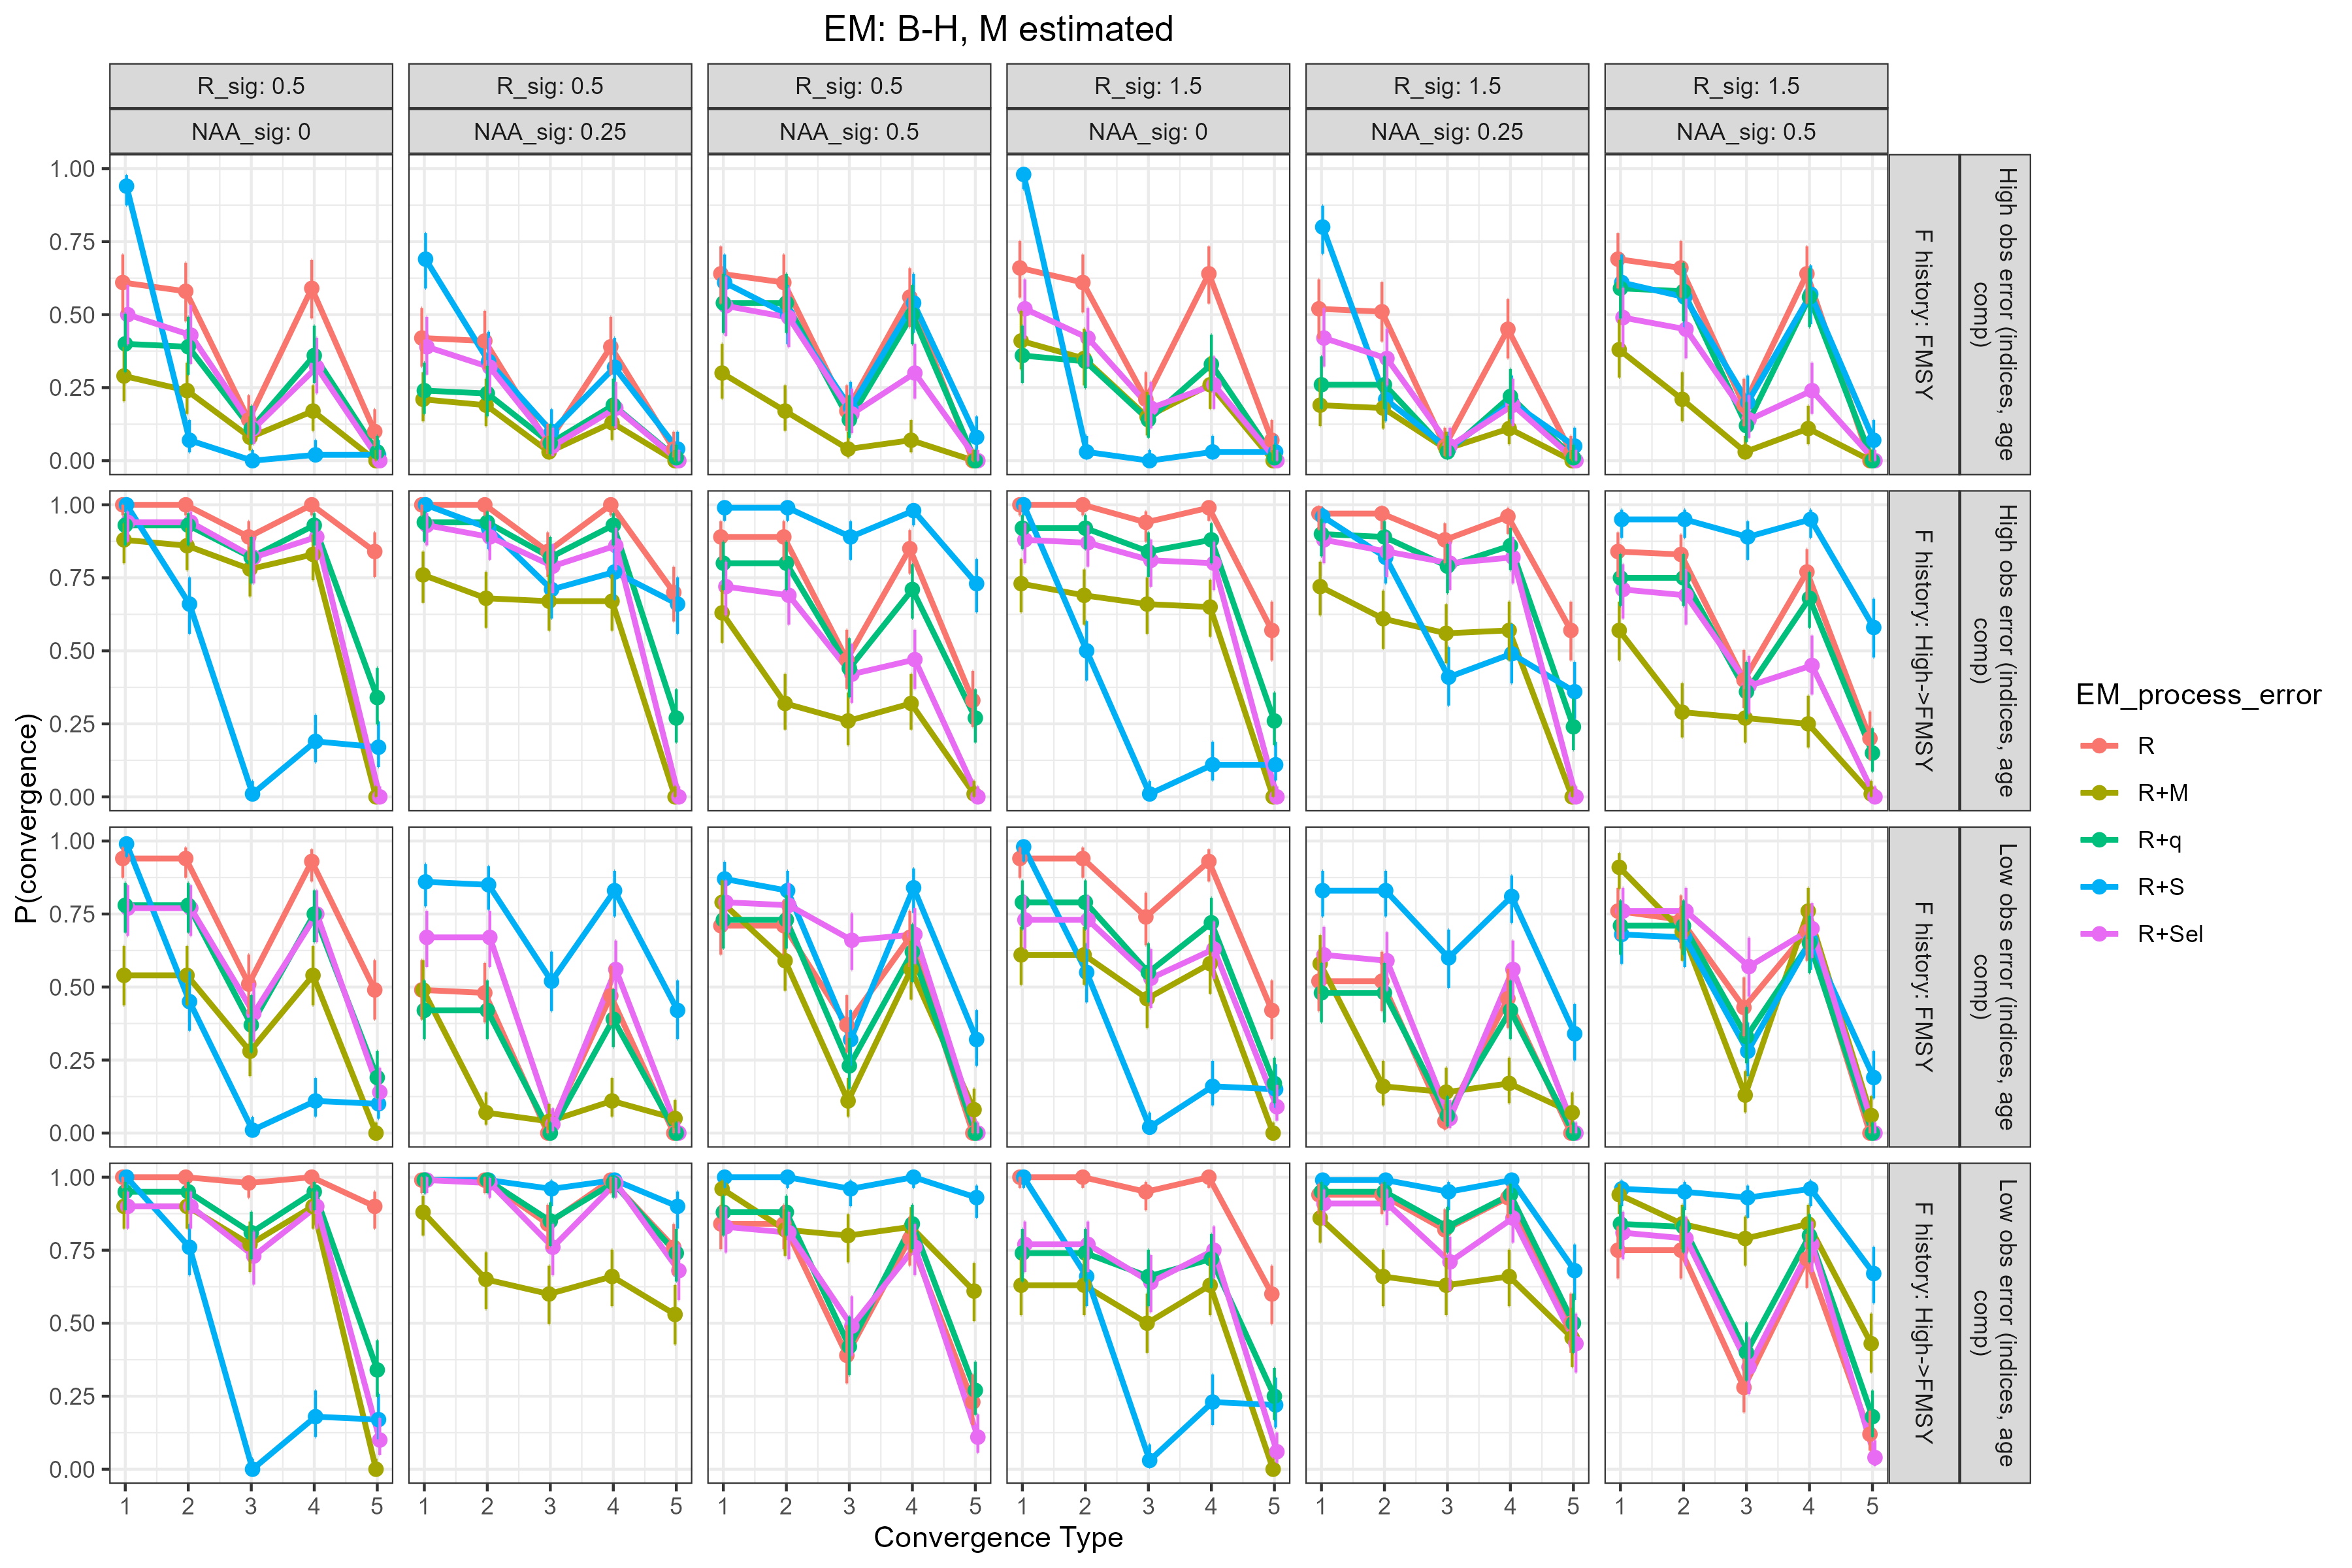
\includegraphics[width = \textwidth]{naa_om_p_convergence_BH_M_estimated.png}
\end{center}
\end{figure}
\end{landscape}

\begin{landscape}
\begin{figure}
\caption{Probability of each type of convergence of estimating models with alternative process error assumptions for operating models that have process error structure R+M. vertical lines represent 95\% confidence intervals. All estimating models estimate mean recruitment rather than a stock-recruit relationship and and M is fixed at the true value.}\label{M_om_em_R_MF_convergence}
\begin{center}
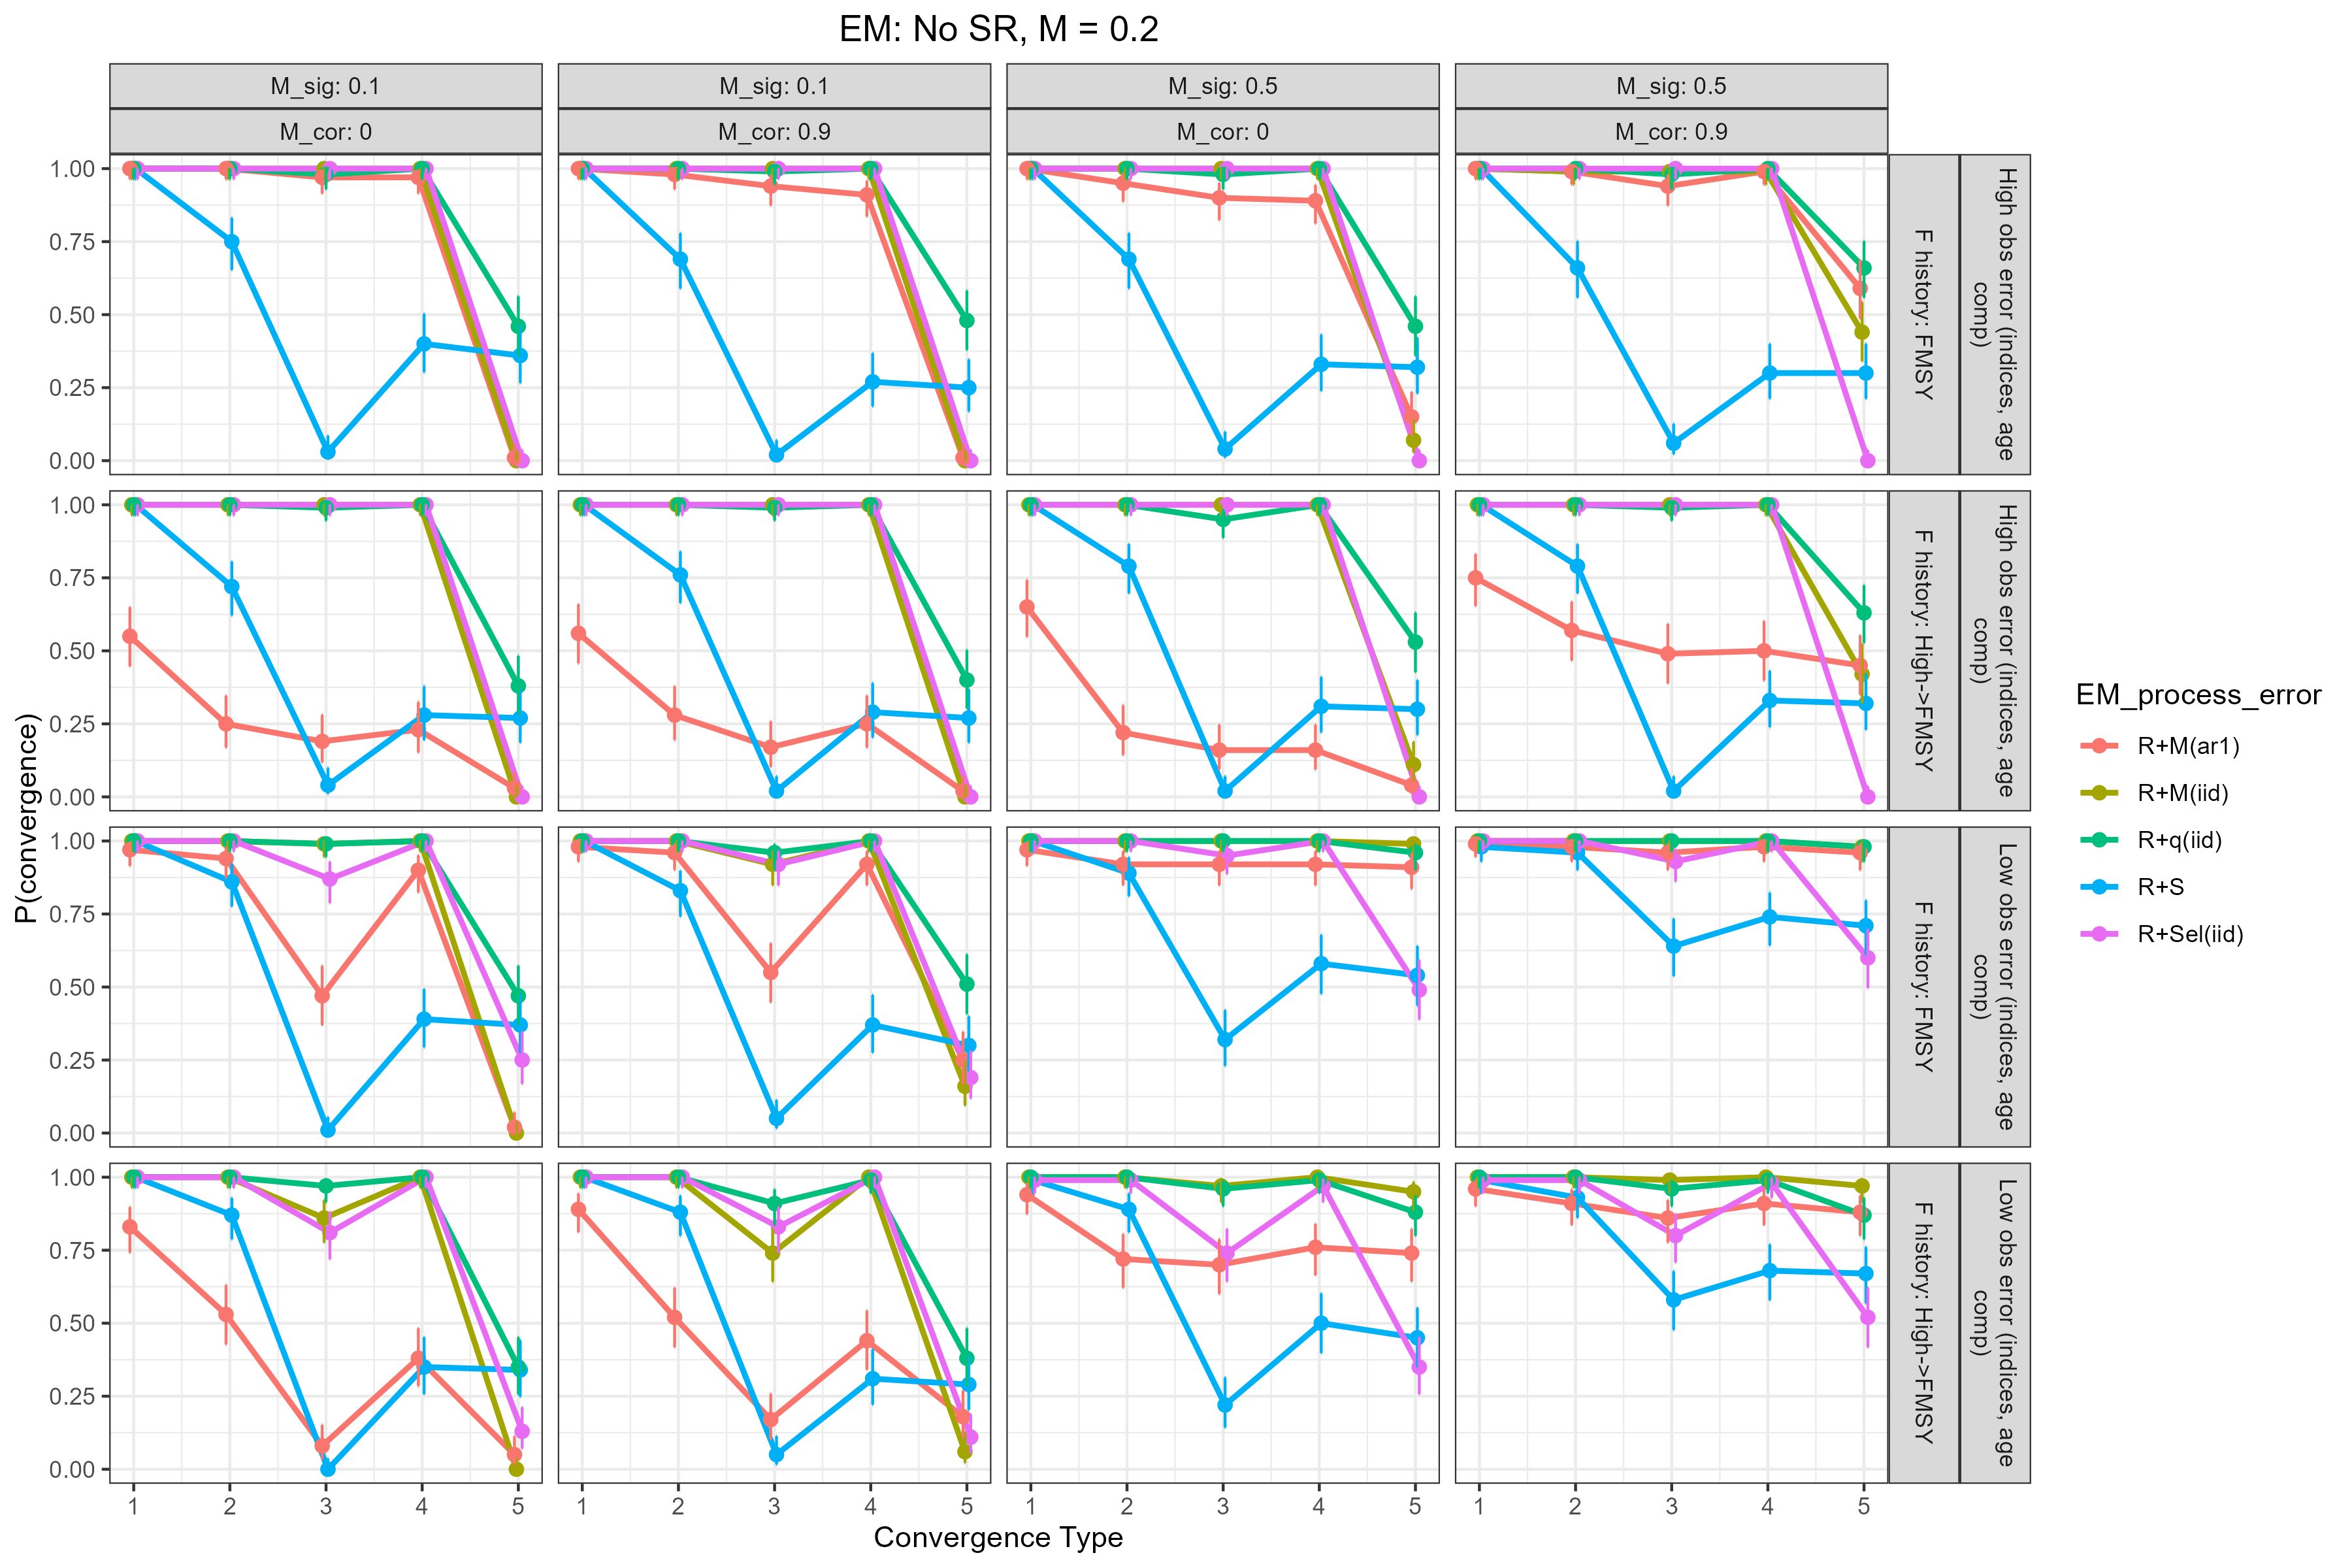
\includegraphics[width = \textwidth]{M_om_p_convergence_meanR_M_fixed.png}
\end{center}
\end{figure}
\end{landscape}

\begin{landscape}
\begin{figure}
\caption{Probability of each type of convergence of estimating models with alternative process error assumptions for operating models that have process error structure R+M. vertical lines represent 95\% confidence intervals. All estimating models estimate mean recruitment rather than a stock-recruit relationship and and M is estimated.}\label{M_om_em_R_ME_convergence}
\begin{center}
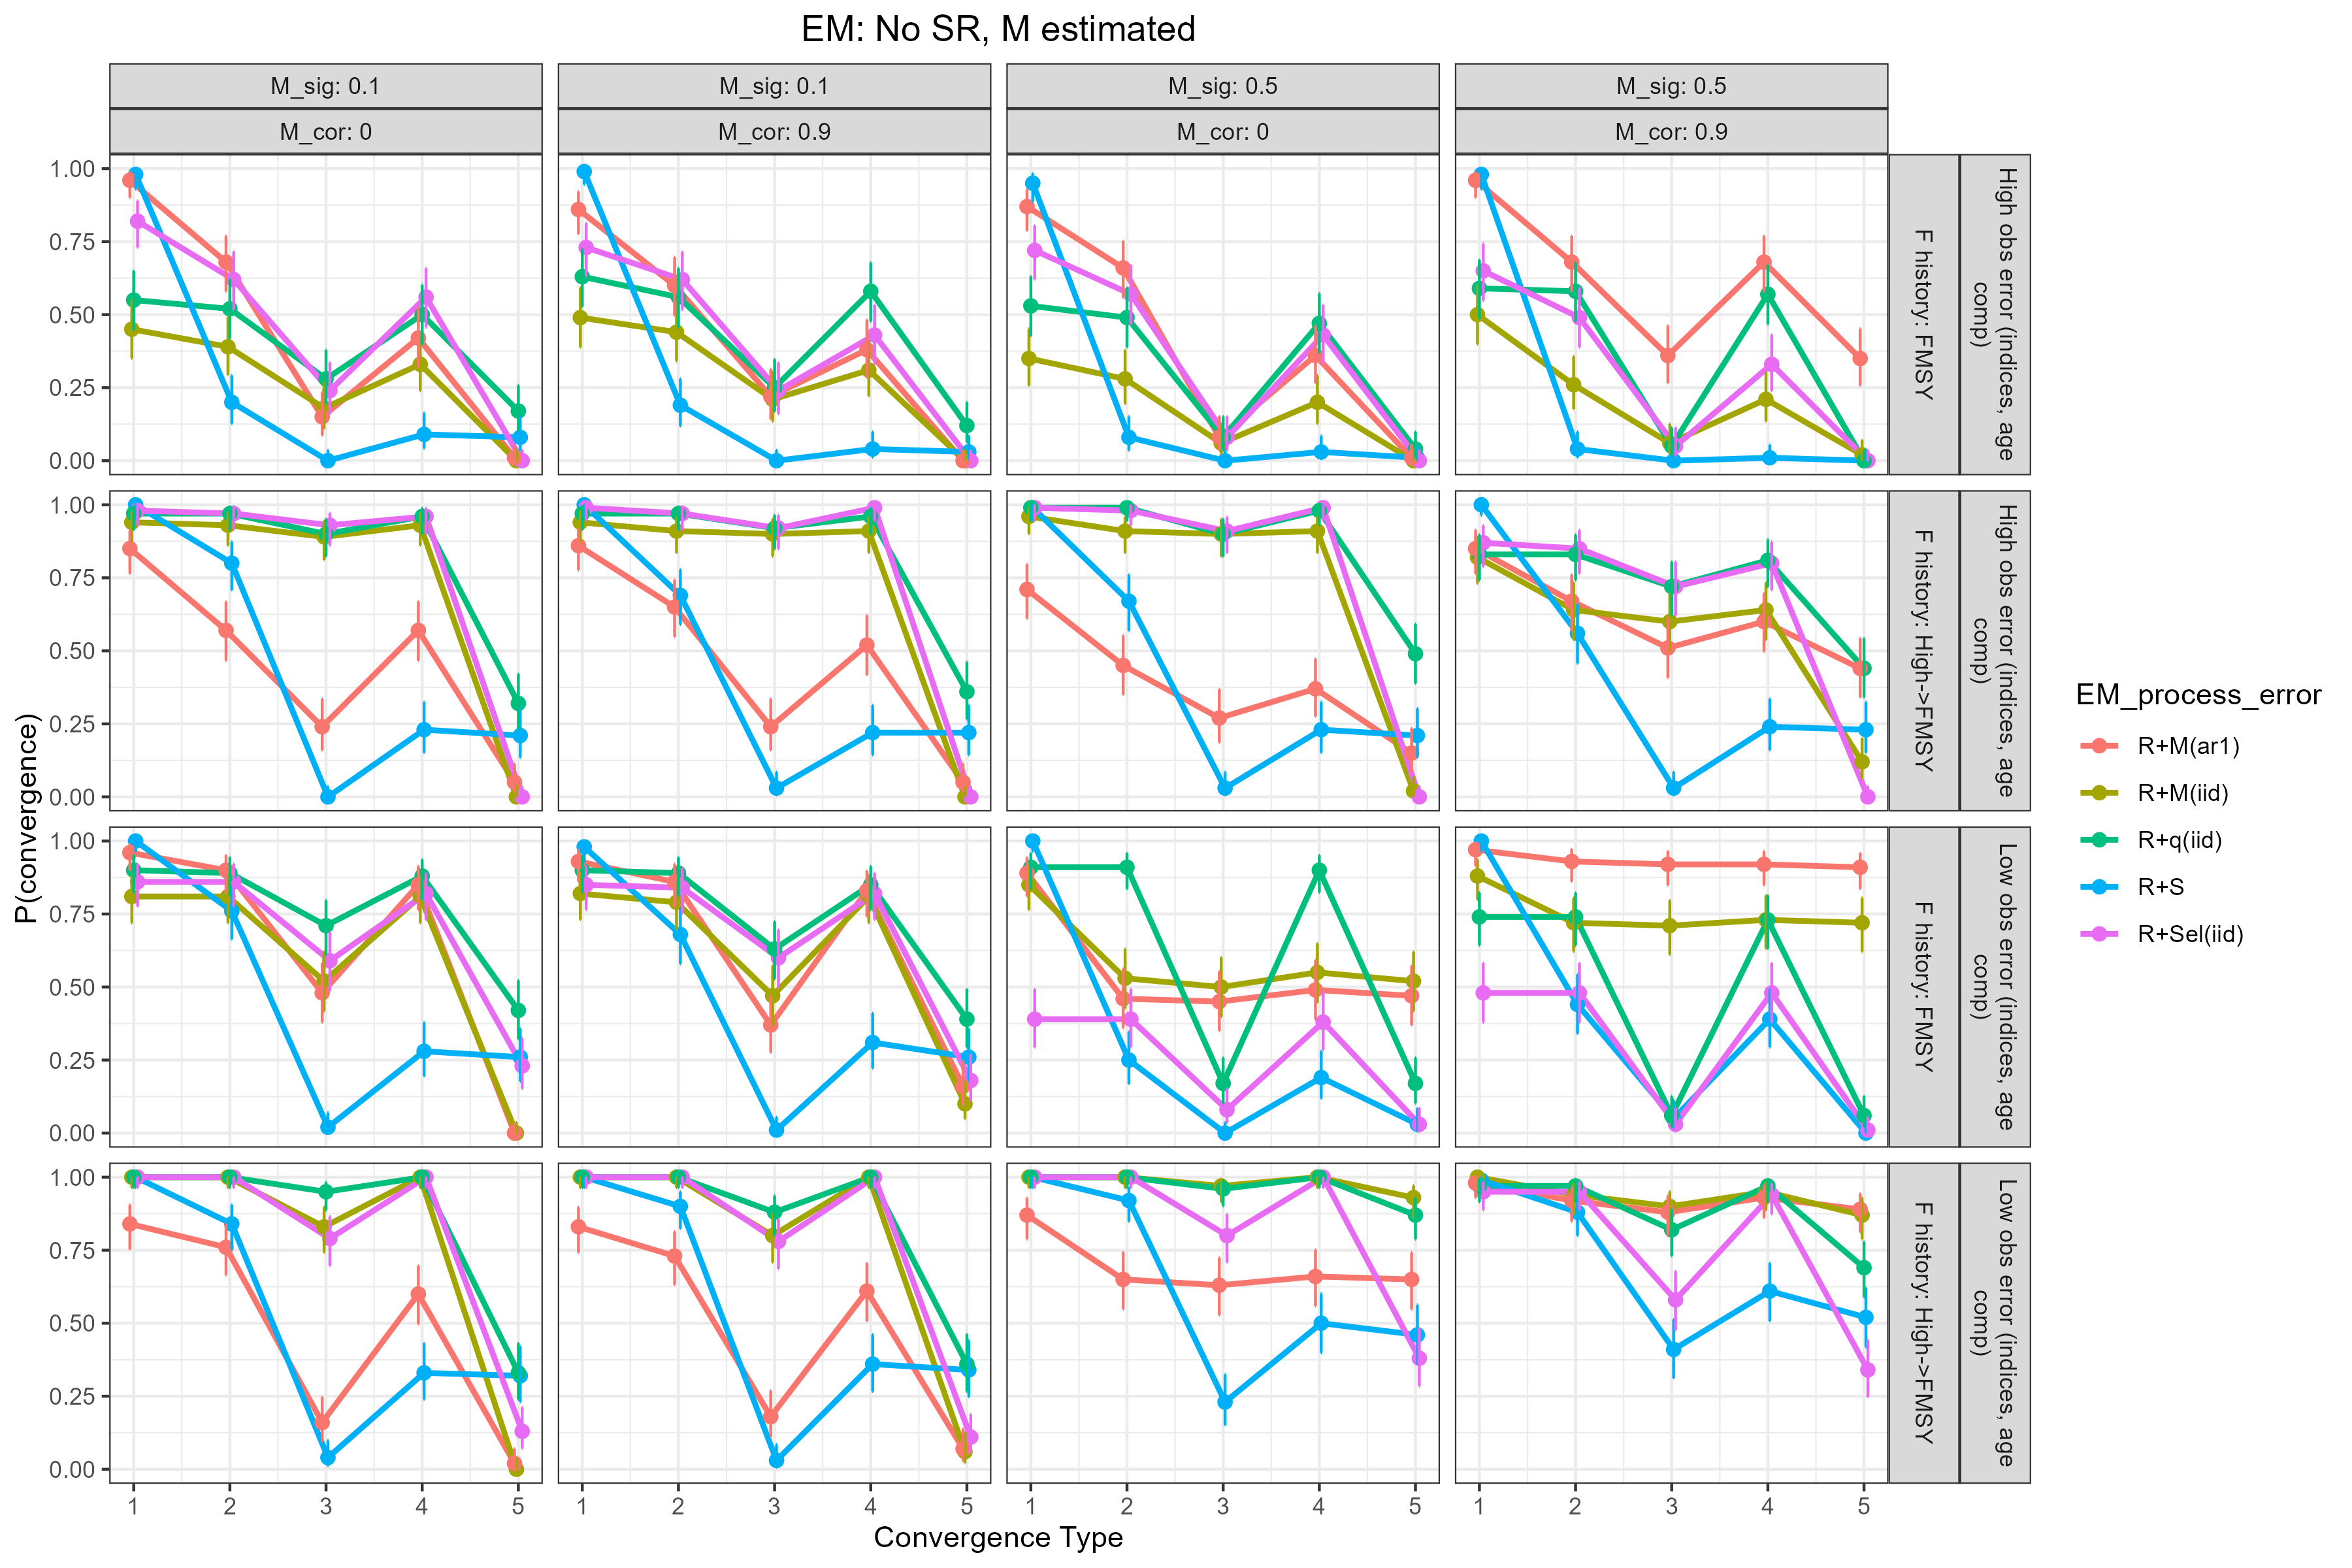
\includegraphics[width = \textwidth]{M_om_p_convergence_meanR_M_estimated.png}
\end{center}
\end{figure}
\end{landscape}

\begin{landscape}
\begin{figure}
\caption{Probability of each type of convergence of estimating models with alternative process error assumptions for operating models that have process error structure R+M. vertical lines represent 95\% confidence intervals. All estimating models estimate a Beverton-Holt stock-recruit relationship and and M is fixed at the true value.}\label{M_om_em_BH_MF_convergence}
\begin{center}
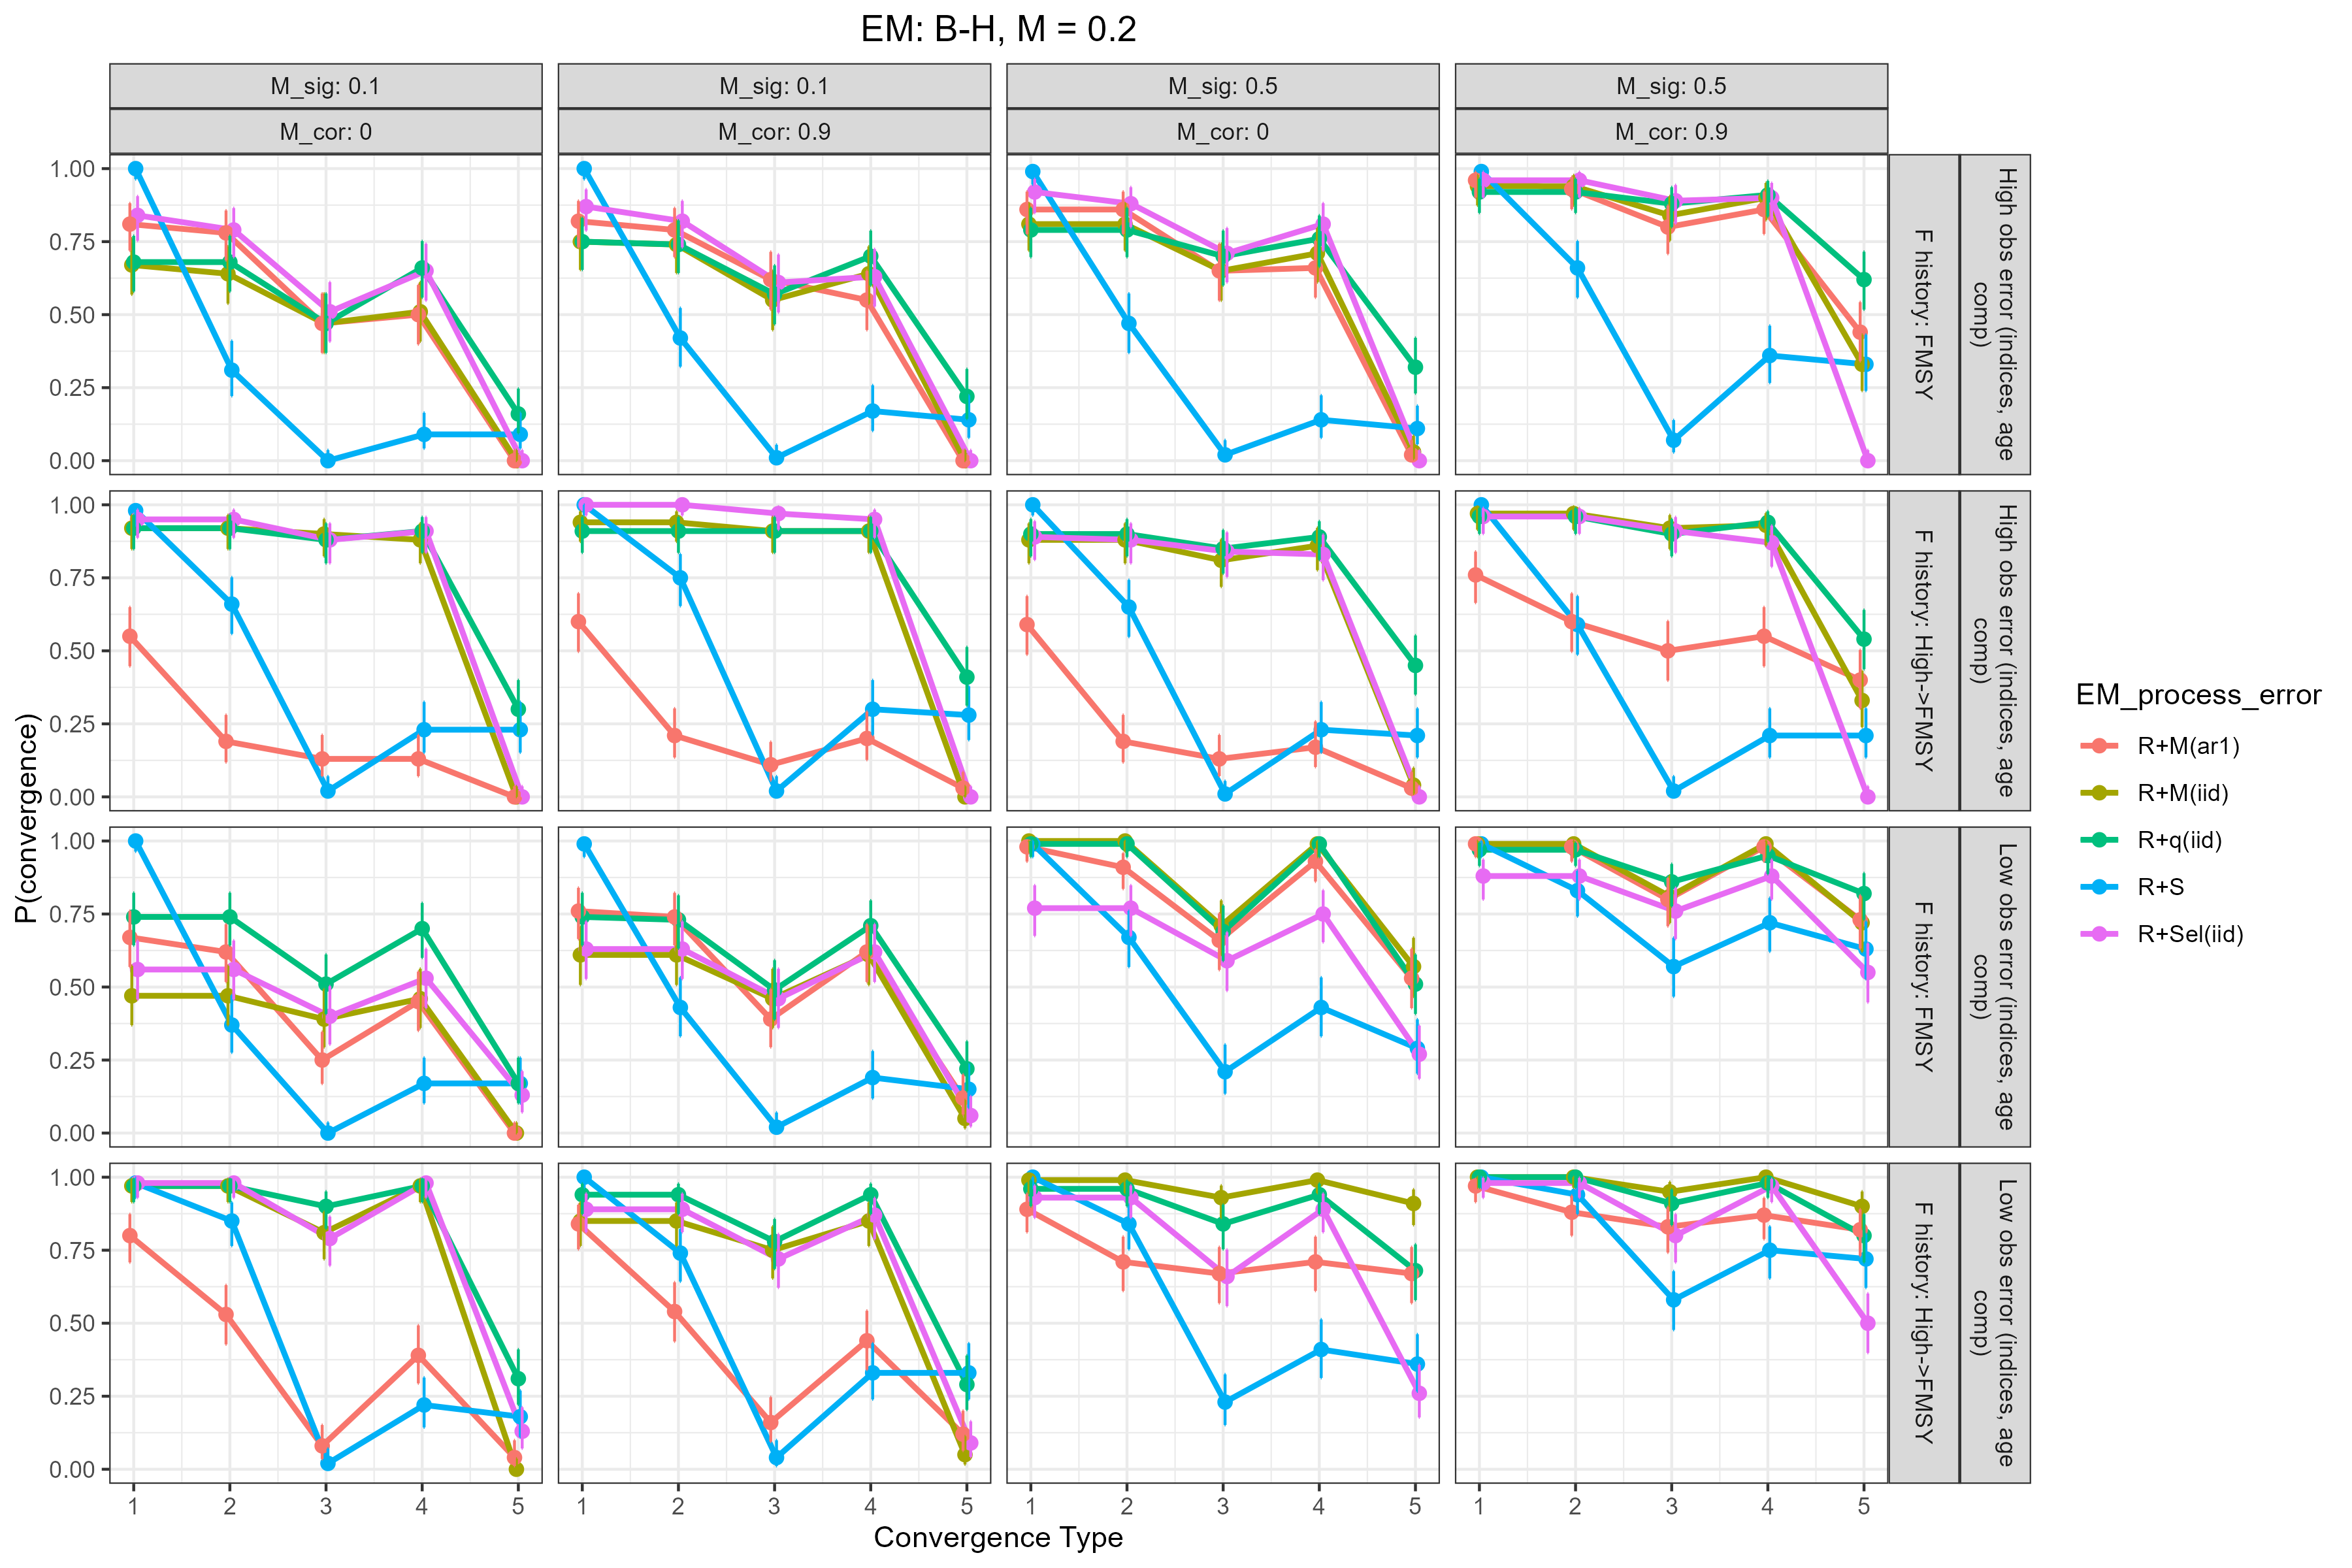
\includegraphics[width = \textwidth]{M_om_p_convergence_BH_M_fixed.png}
\end{center}
\end{figure}
\end{landscape}

\begin{landscape}
\begin{figure}
\caption{Probability of each type of convergence of estimating models with alternative process error assumptions for operating models that have process error structure R+M. vertical lines represent 95\% confidence intervals. All estimating models estimate a Beverton-Holt stock-recruit relationship and and M is estimated.}\label{M_om_em_BH_ME_convergence}
\begin{center}
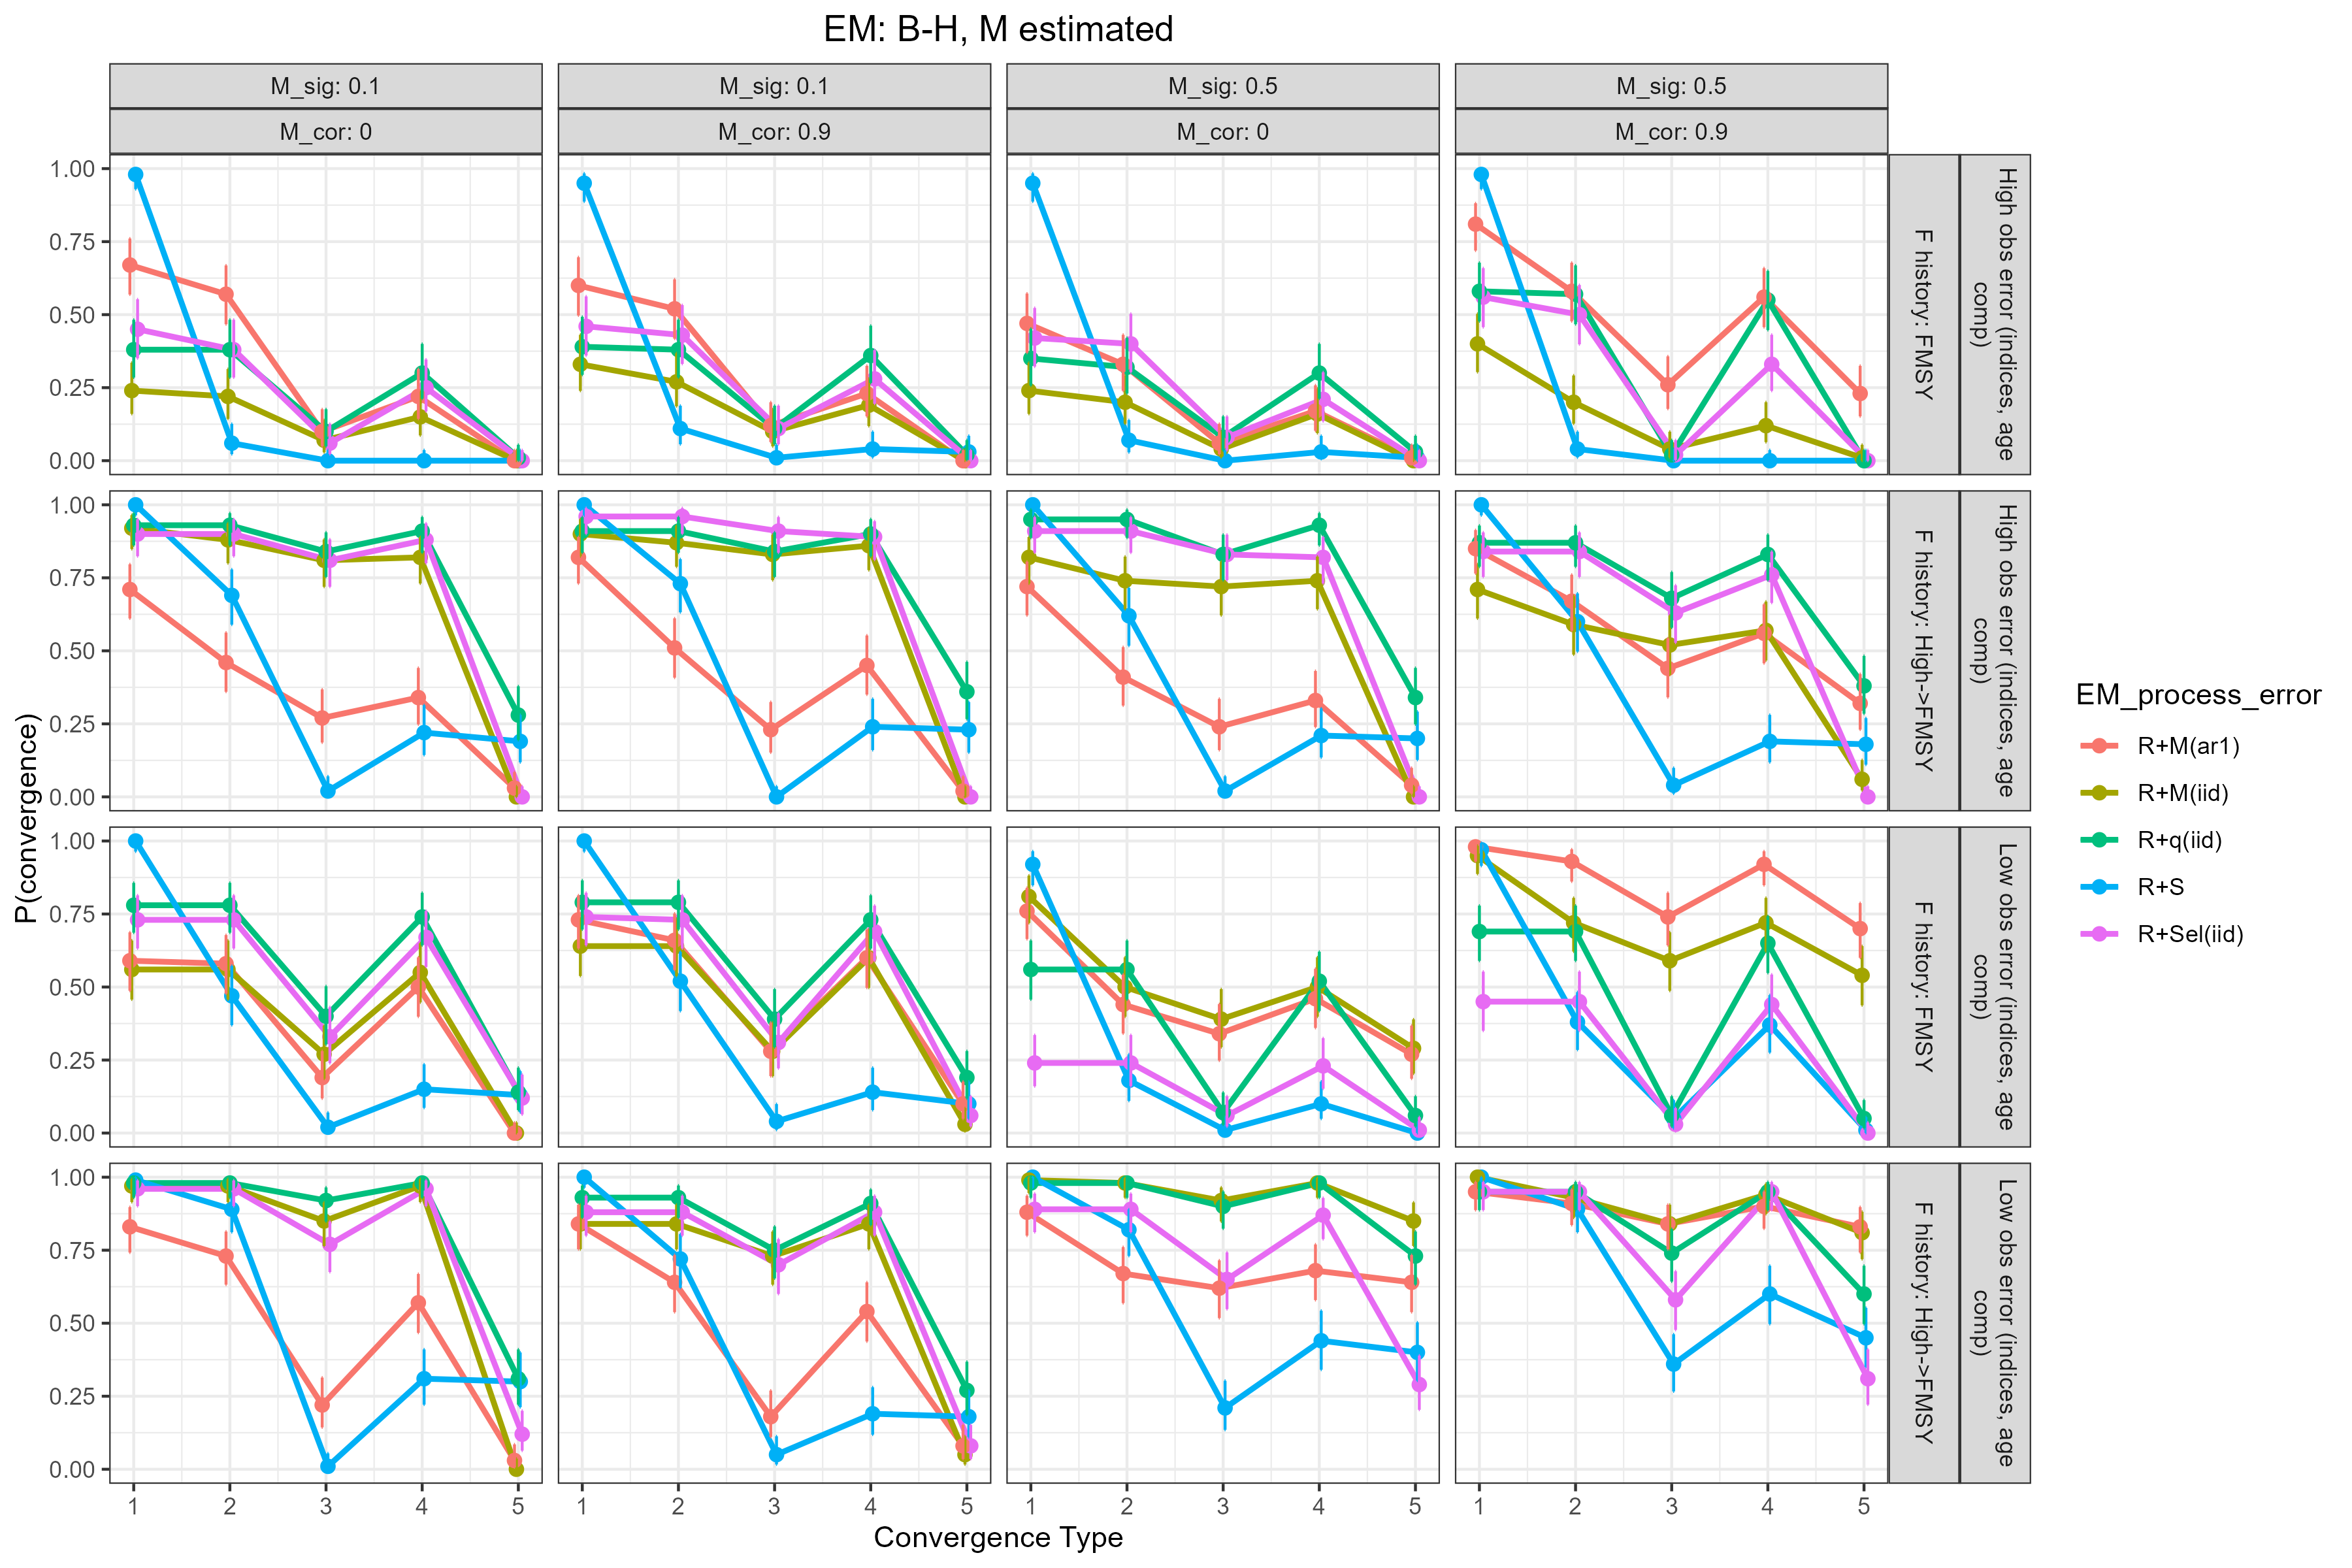
\includegraphics[width = \textwidth]{M_om_p_convergence_BH_M_estimated.png}
\end{center}
\end{figure}
\end{landscape}

\begin{landscape}
\begin{figure}
\caption{Probability of each type of convergence of estimating models with alternative process error assumptions for operating models that have process error structure R+Sel. vertical lines represent 95\% confidence intervals. All estimating models estimate mean recruitment rather than a stock-recruit relationship and and M is fixed at the true value.}\label{Sel_om_em_R_MF_convergence}
\begin{center}
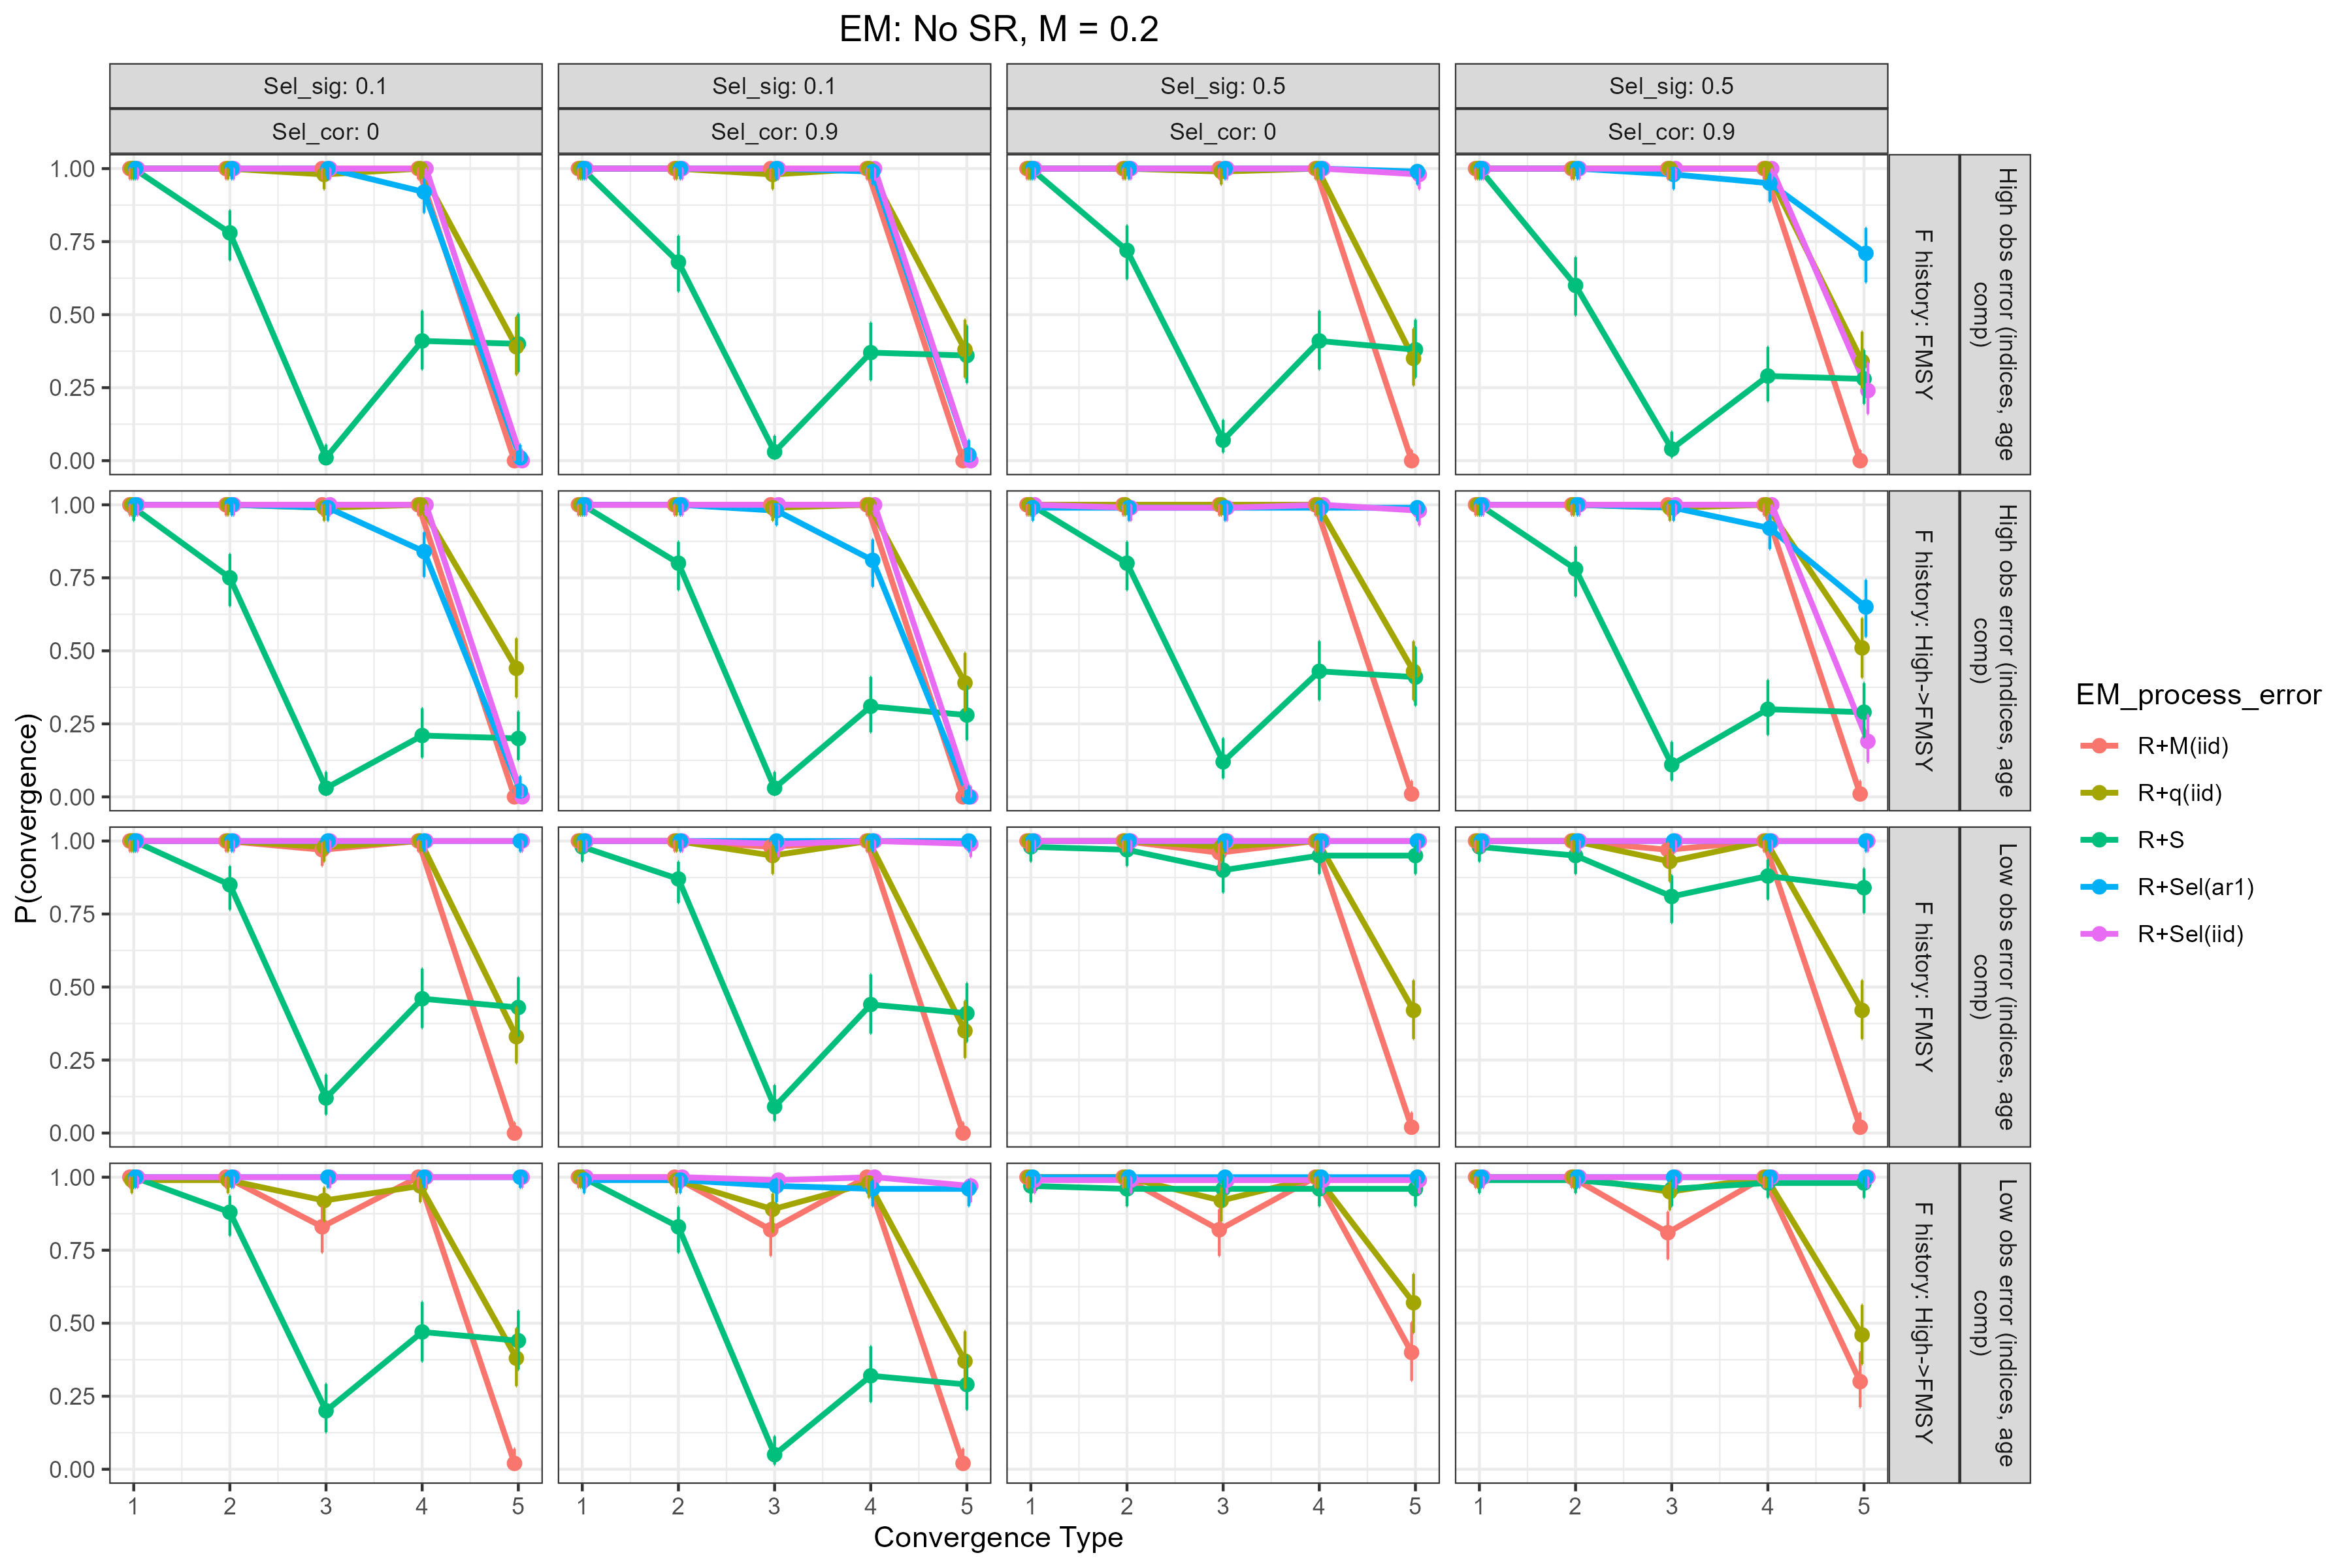
\includegraphics[width = \textwidth]{Sel_om_p_convergence_meanR_M_fixed.png}
\end{center}
\end{figure}
\end{landscape}

\begin{landscape}
\begin{figure}
\caption{Probability of each type of convergence of estimating models with alternative process error assumptions for operating models that have process error structure R+Sel. vertical lines represent 95\% confidence intervals. All estimating models estimate mean recruitment rather than a stock-recruit relationship and and M is estimated.}\label{Sel_om_em_R_ME_convergence}
\begin{center}
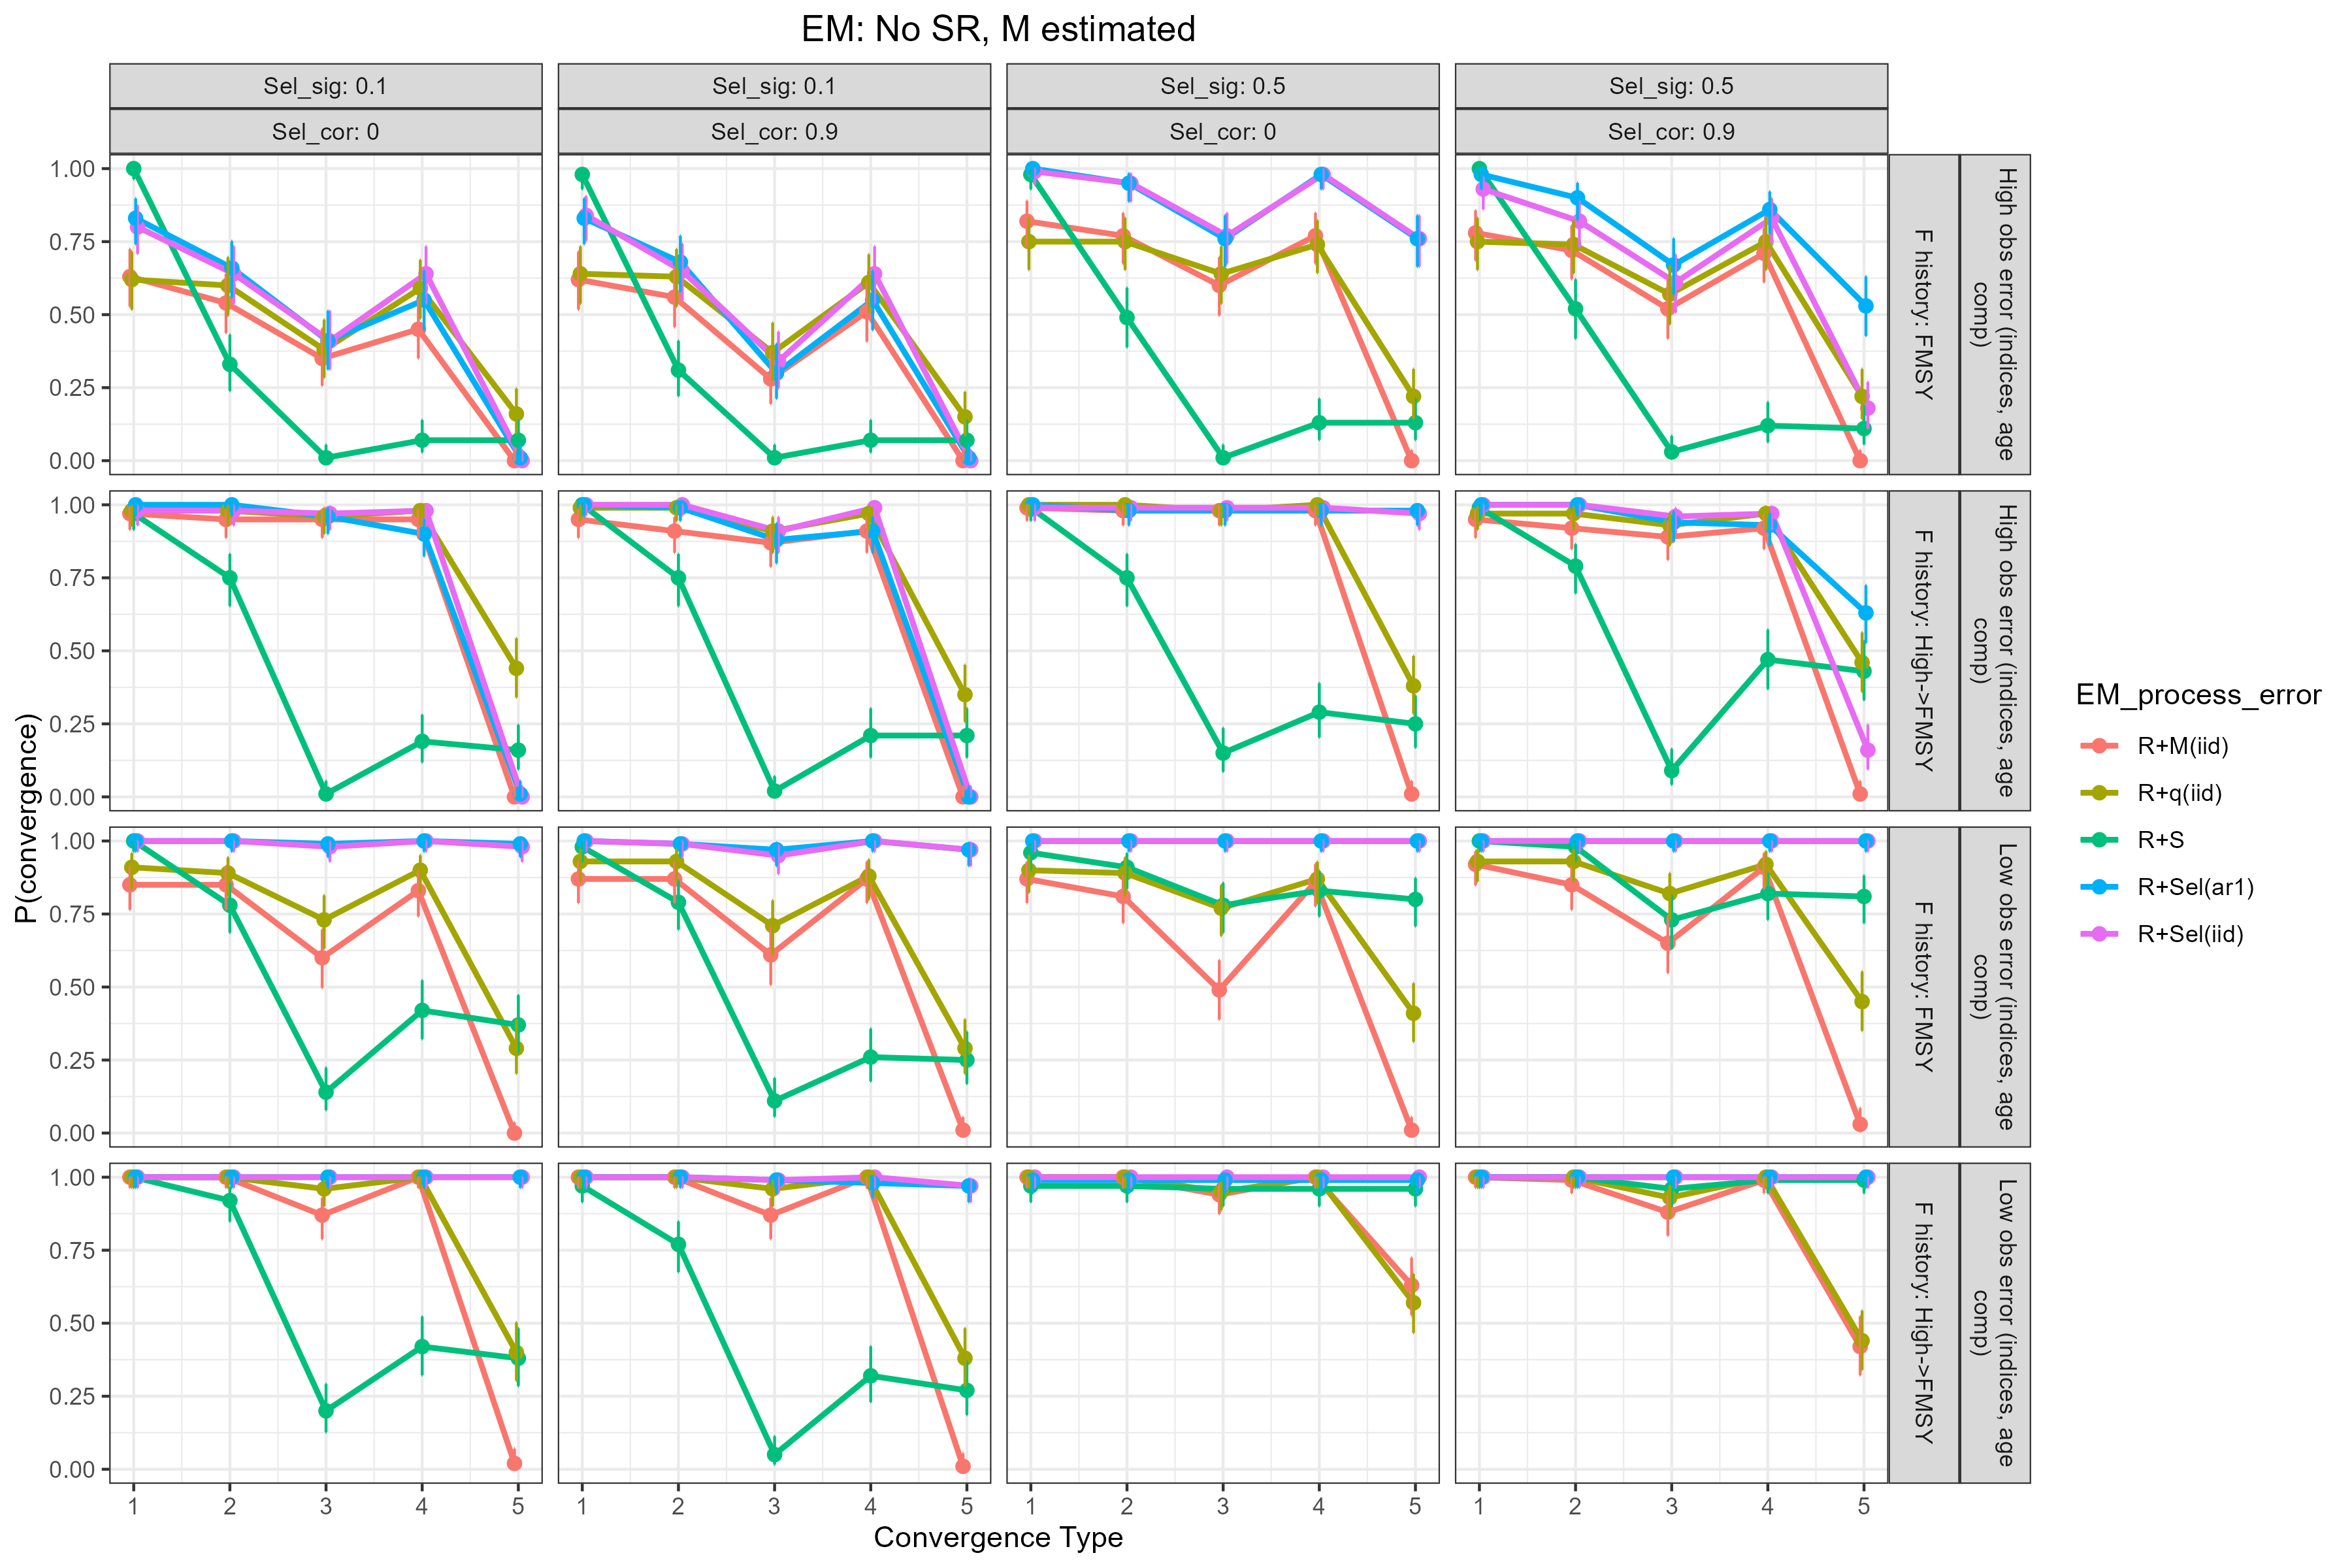
\includegraphics[width = \textwidth]{Sel_om_p_convergence_meanR_M_estimated.png}
\end{center}
\end{figure}
\end{landscape}

\begin{landscape}
\begin{figure}
\caption{Probability of each type of convergence of estimating models with alternative process error assumptions for operating models that have process error structure R+Sel. vertical lines represent 95\% confidence intervals. All estimating models estimate a Beverton-Holt stock-recruit relationship and and M is fixed at the true value.}\label{Sel_om_em_BH_MF_convergence}
\begin{center}
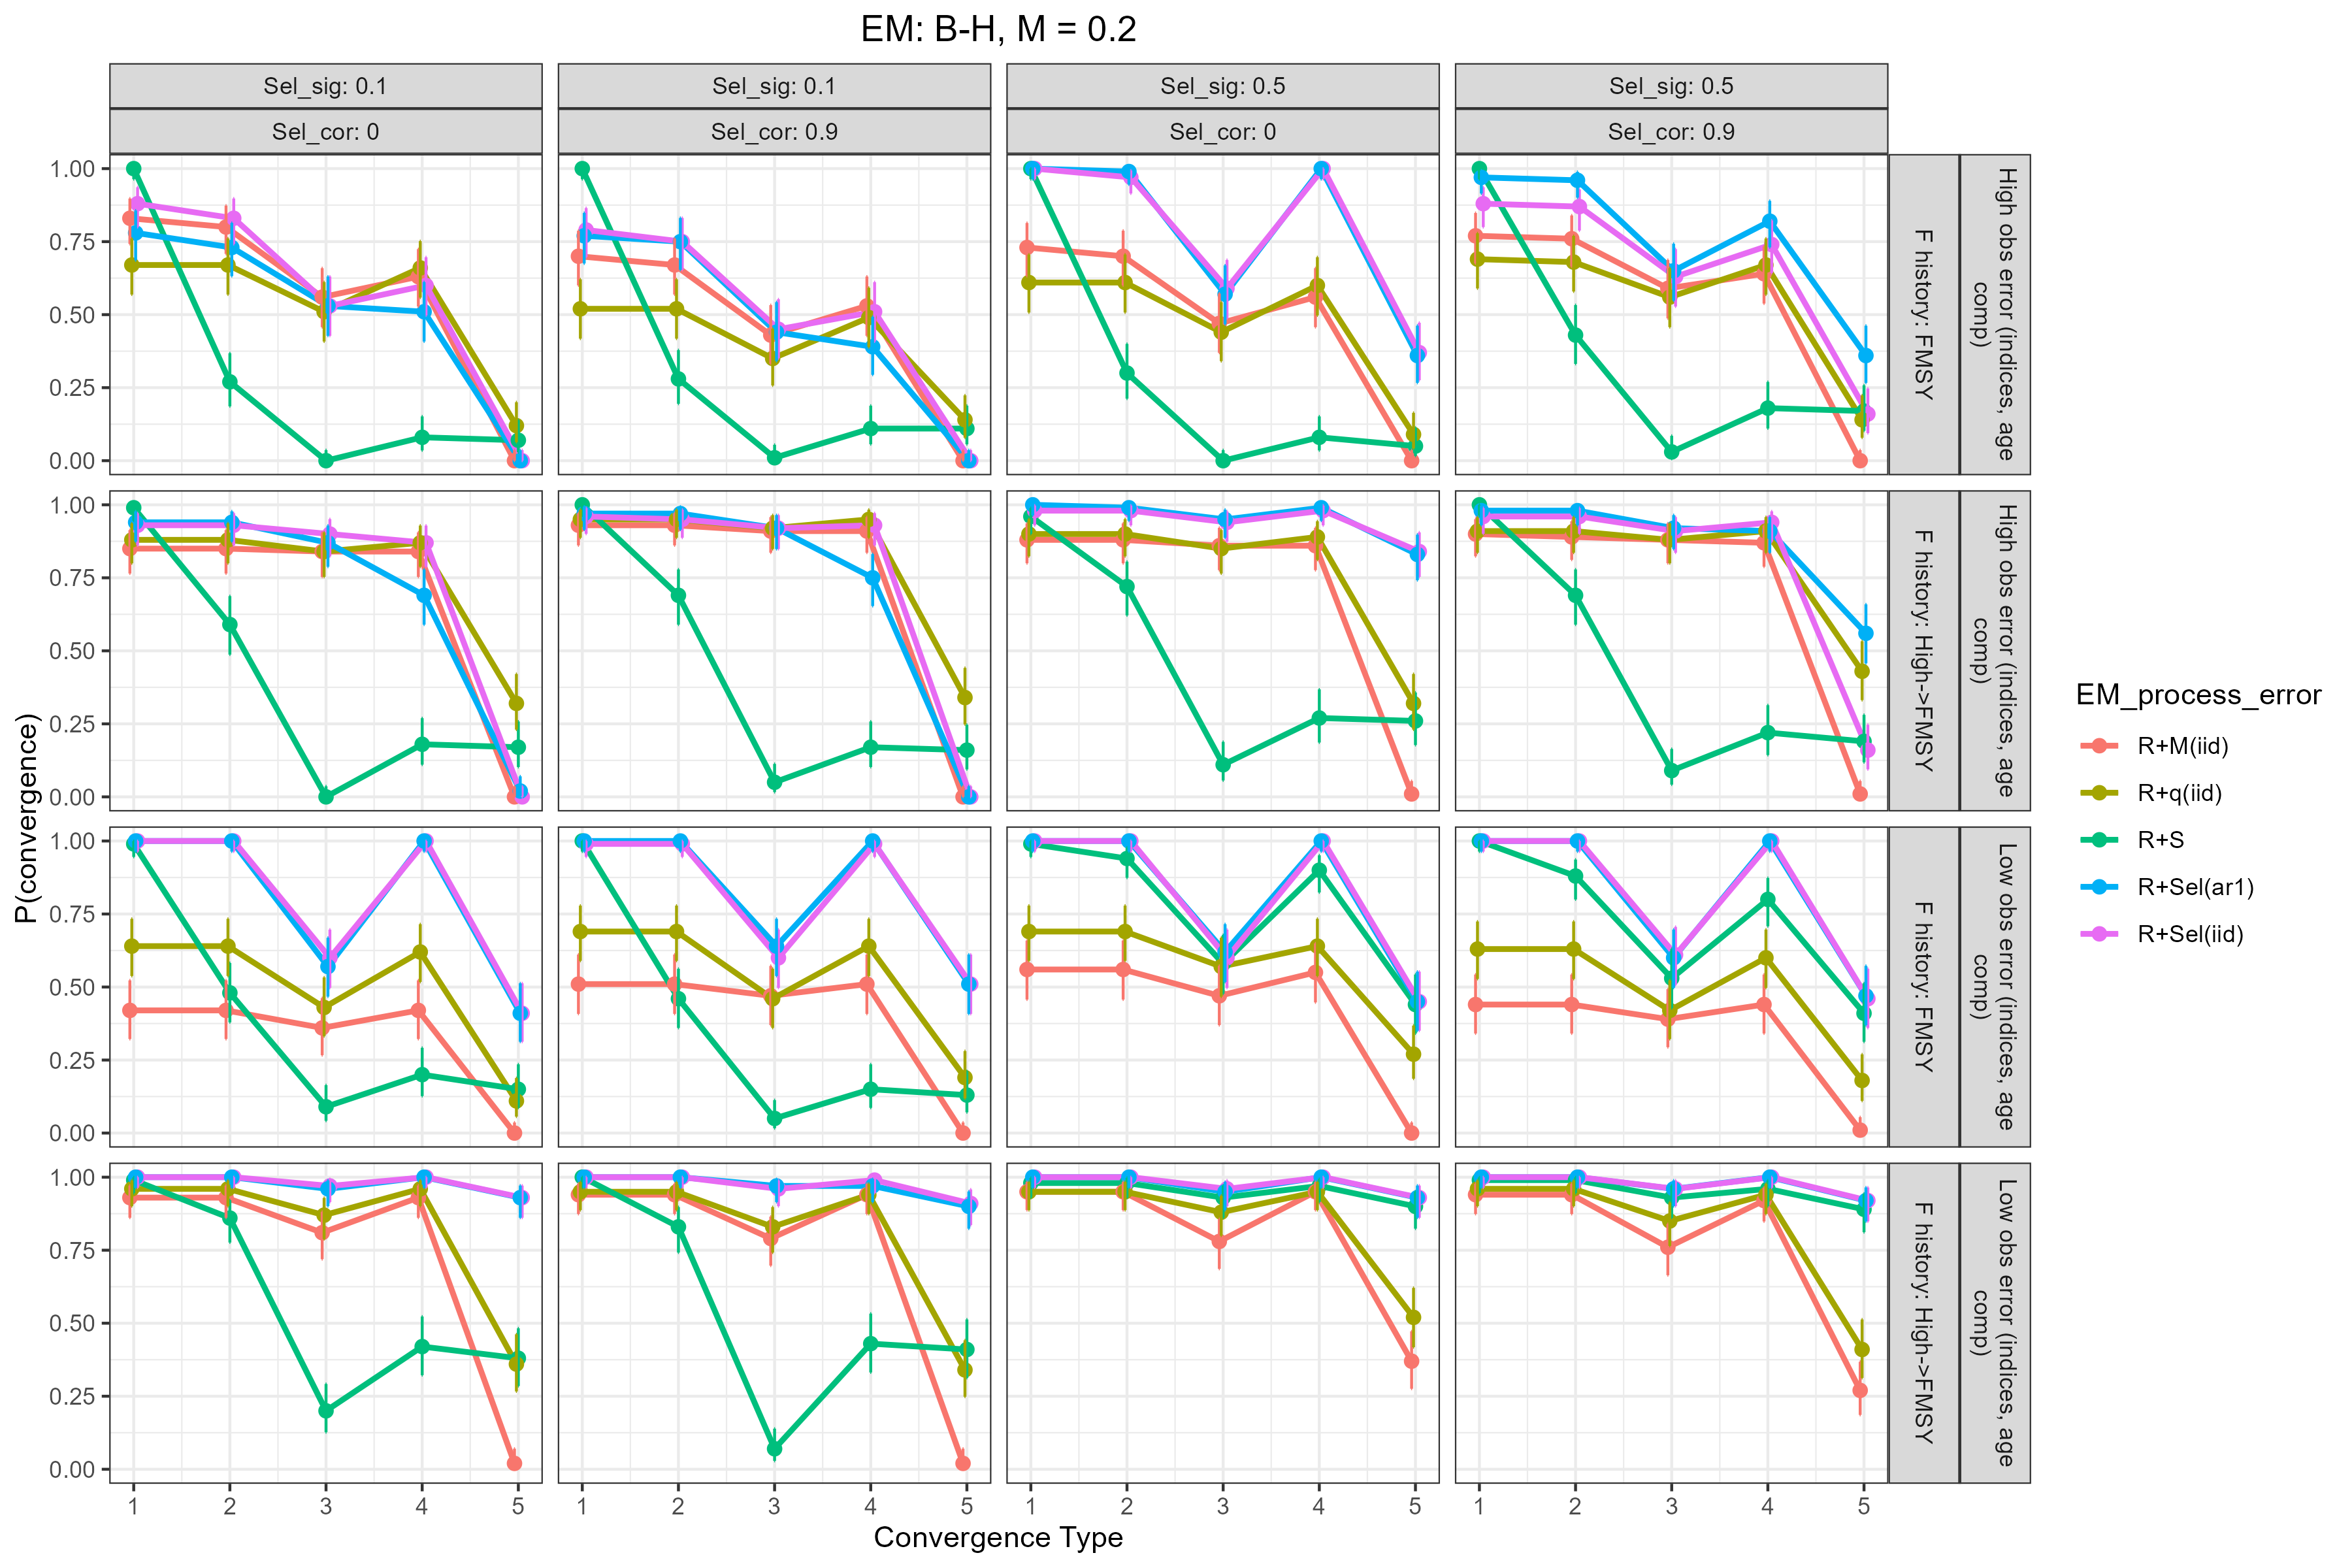
\includegraphics[width = \textwidth]{Sel_om_p_convergence_BH_M_fixed.png}
\end{center}
\end{figure}
\end{landscape}

\begin{landscape}
\begin{figure}
\caption{Probability of each type of convergence of estimating models with alternative process error assumptions for operating models that have process error structure R+Sel. vertical lines represent 95\% confidence intervals. All estimating models estimate a Beverton-Holt stock-recruit relationship and and M is estimated.}\label{Sel_om_em_BH_ME_convergence}
\begin{center}
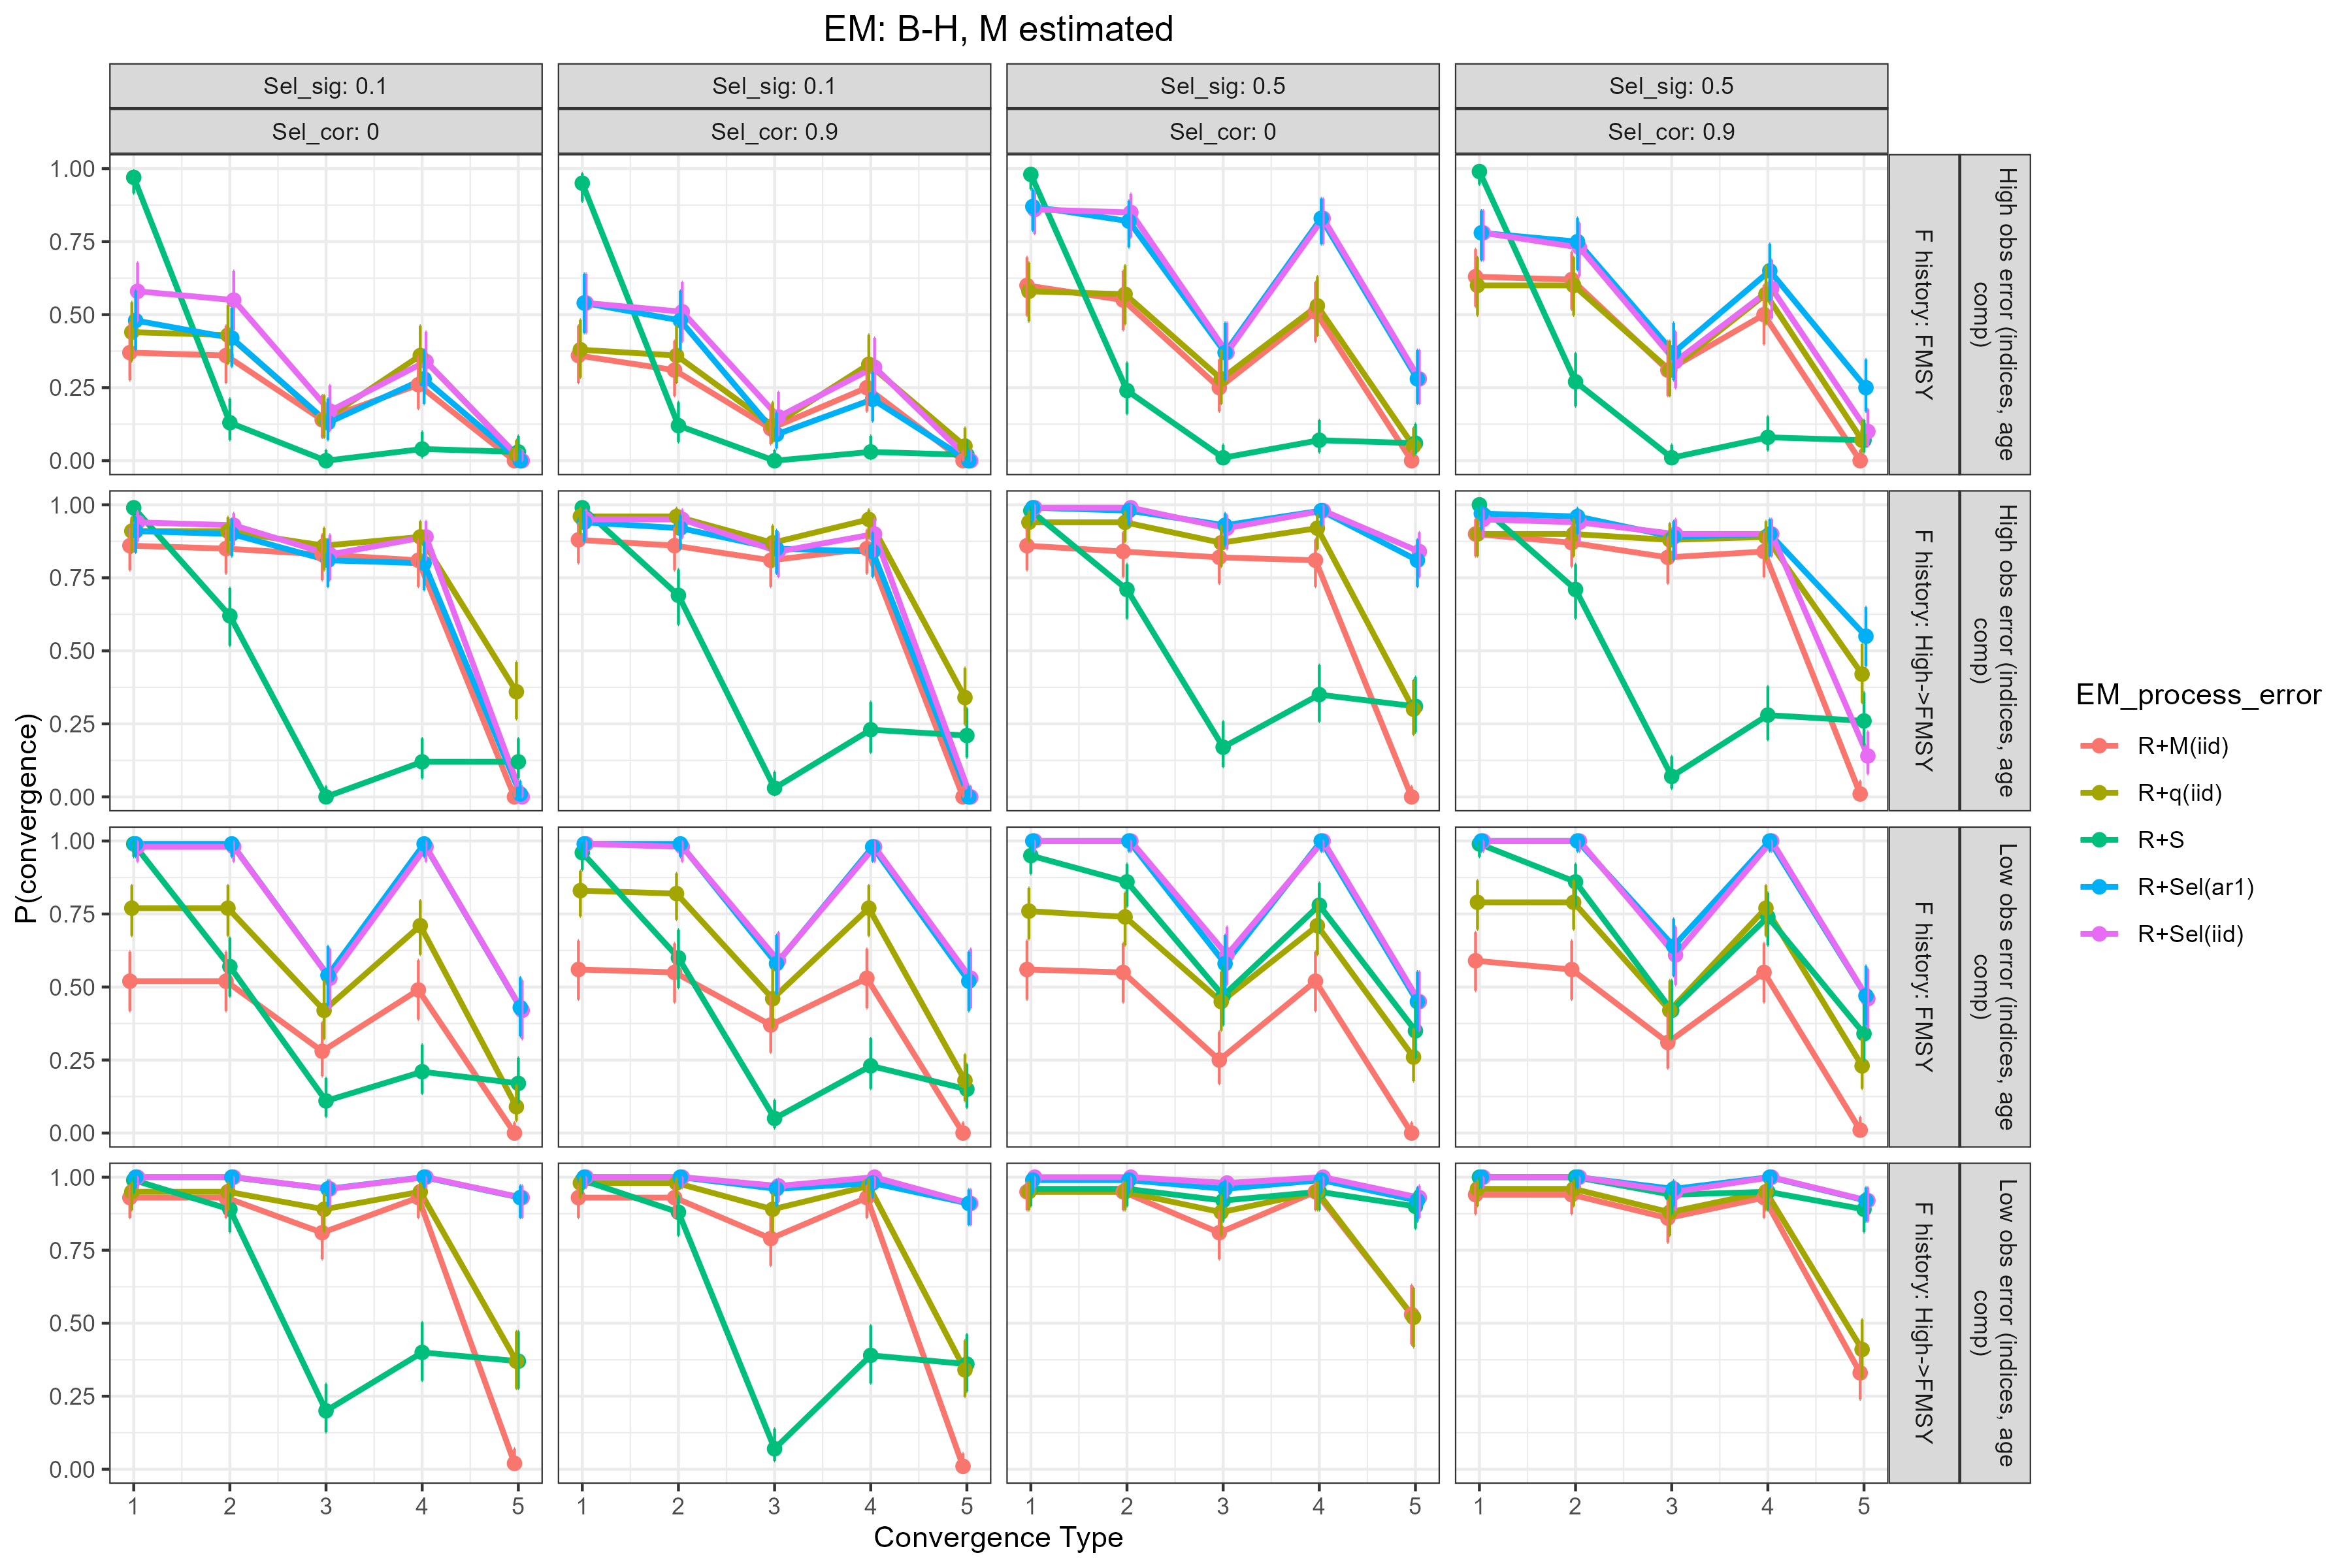
\includegraphics[width = \textwidth]{Sel_om_p_convergence_BH_M_estimated.png}
\end{center}
\end{figure}
\end{landscape}

\begin{landscape}
\begin{figure}
\caption{Probability of each type of convergence of estimating models with alternative process error assumptions for operating models that have process error structure R+q. vertical lines represent 95\% confidence intervals. All estimating models estimate mean recruitment rather than a stock-recruit relationship and and M is fixed at the true value.}\label{q_om_em_R_MF_convergence}
\begin{center}
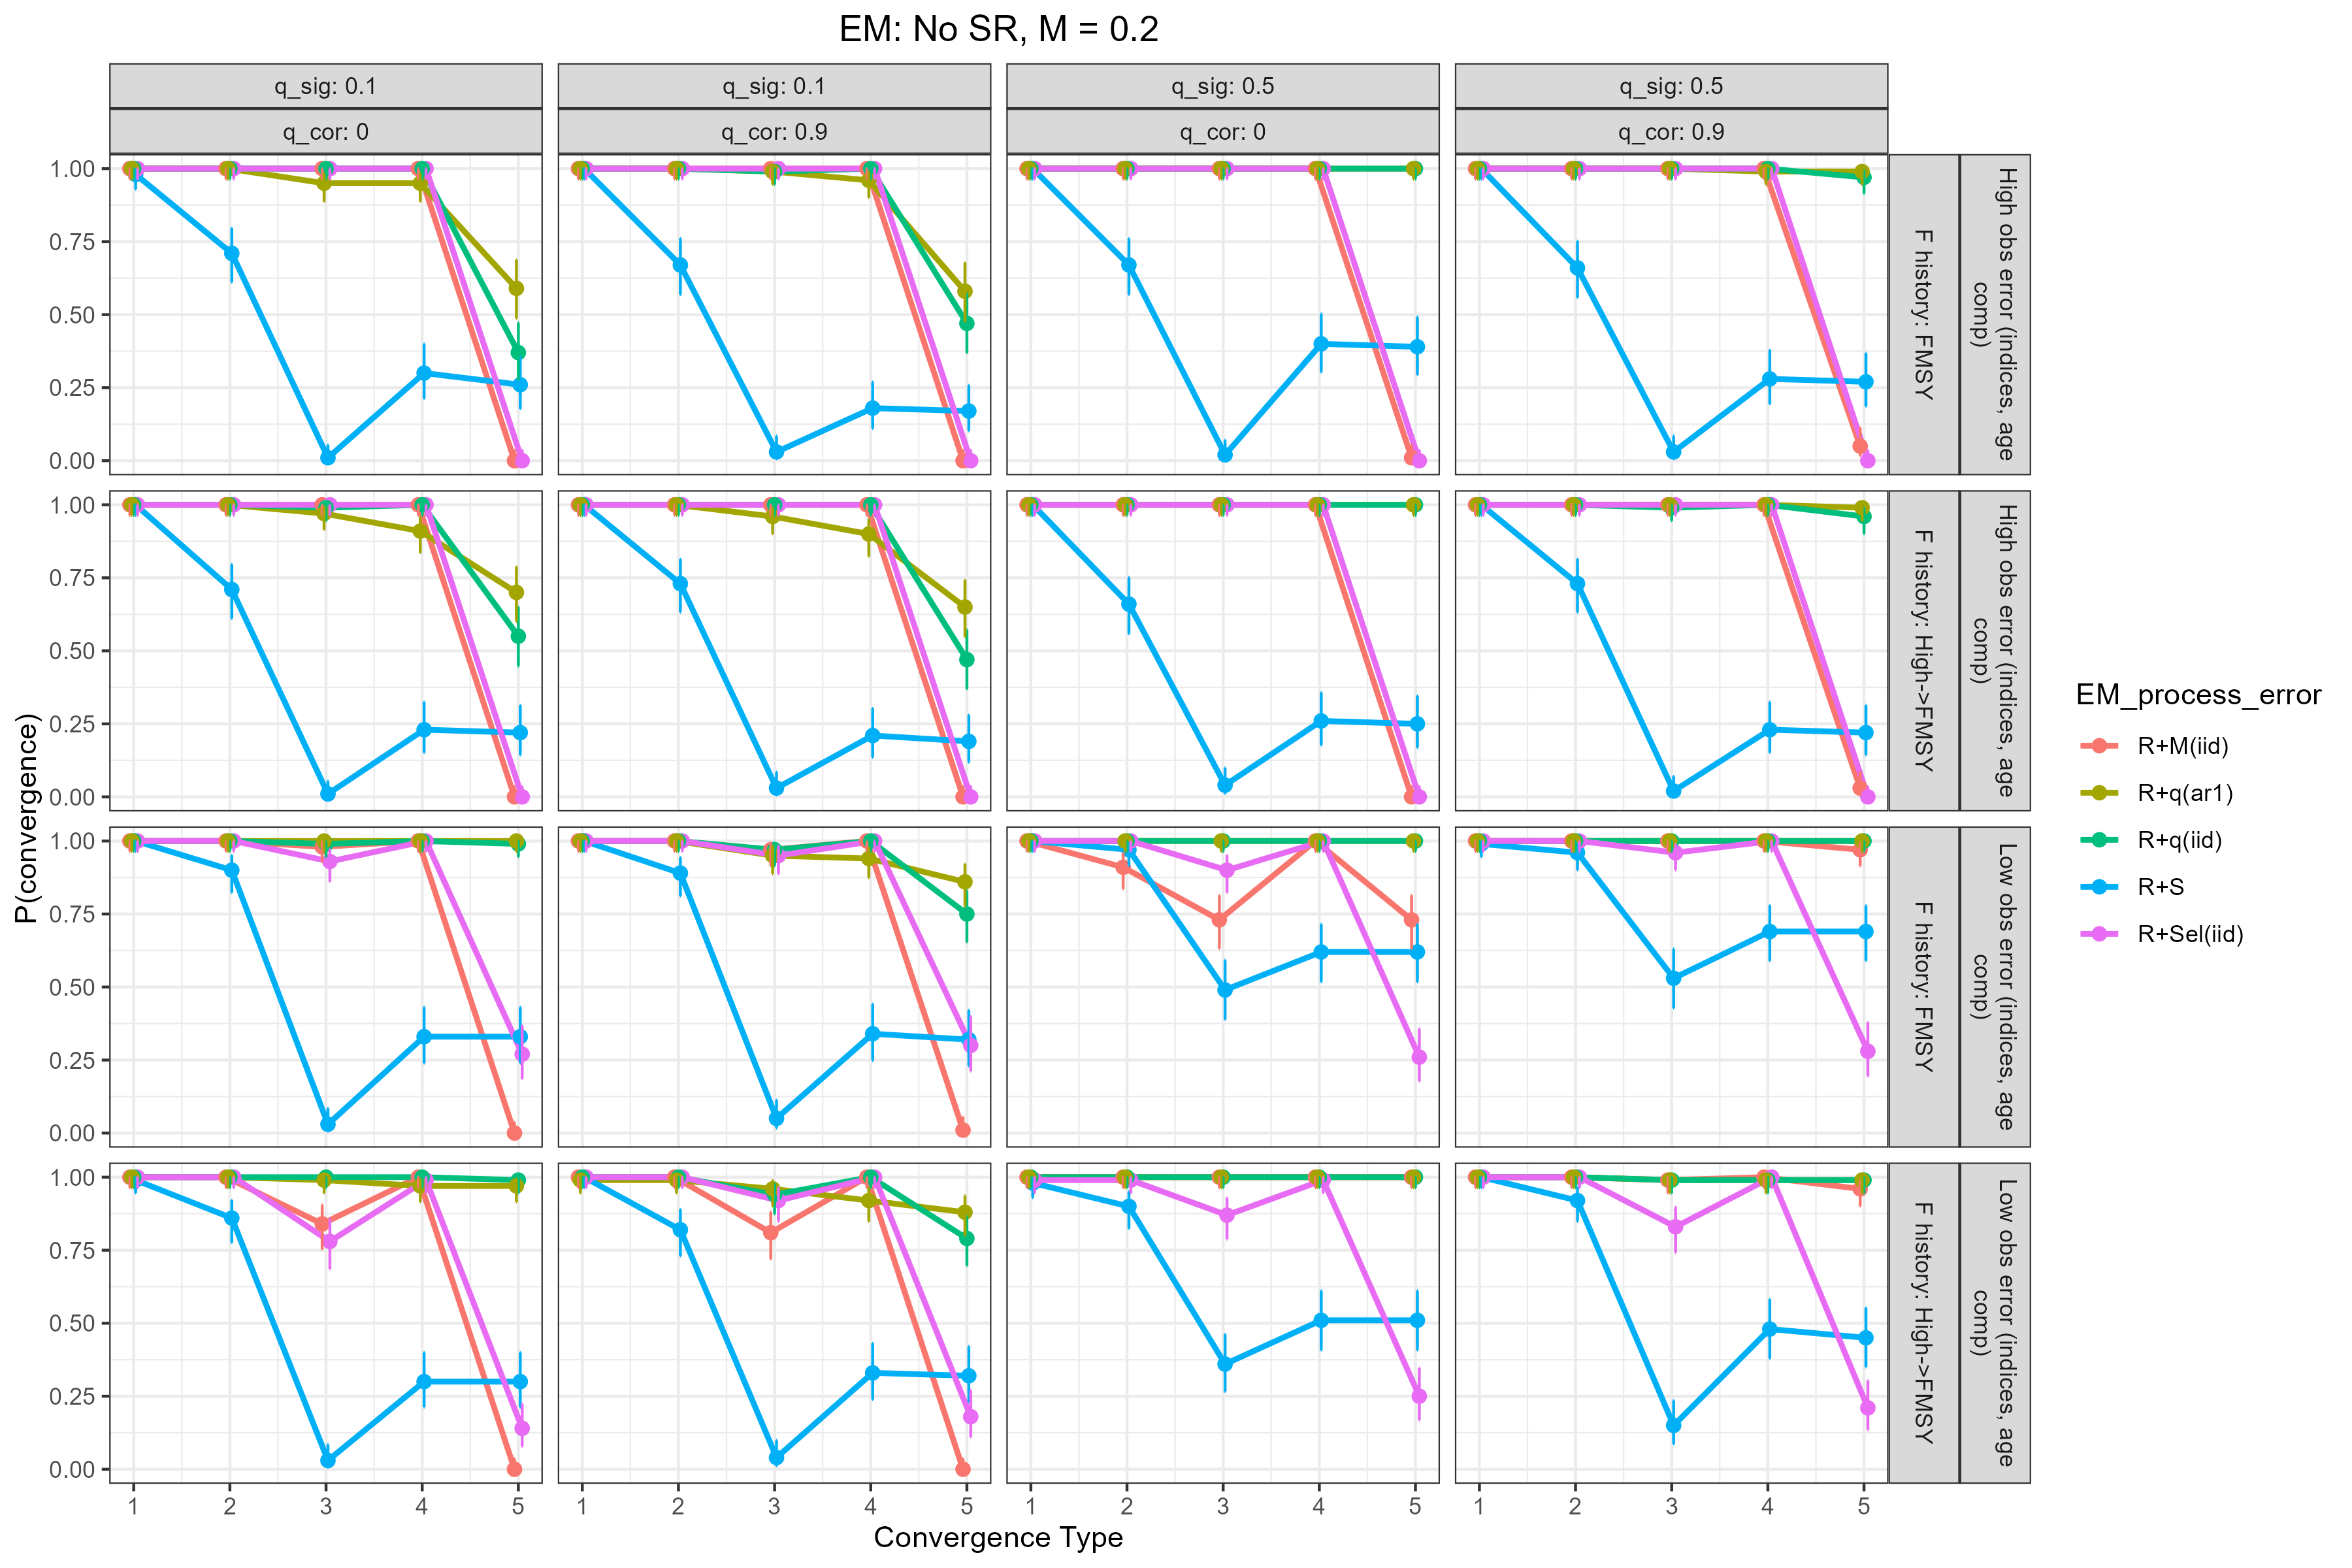
\includegraphics[width = \textwidth]{q_om_p_convergence_meanR_M_fixed.png}
\end{center}
\end{figure}
\end{landscape}

\begin{landscape}
\begin{figure}
\caption{Probability of each type of convergence of estimating models with alternative process error assumptions for operating models that have process error structure R+q. vertical lines represent 95\% confidence intervals. All estimating models estimate mean recruitment rather than a stock-recruit relationship and and M is estimated.}\label{q_om_em_R_ME_convergence}
\begin{center}
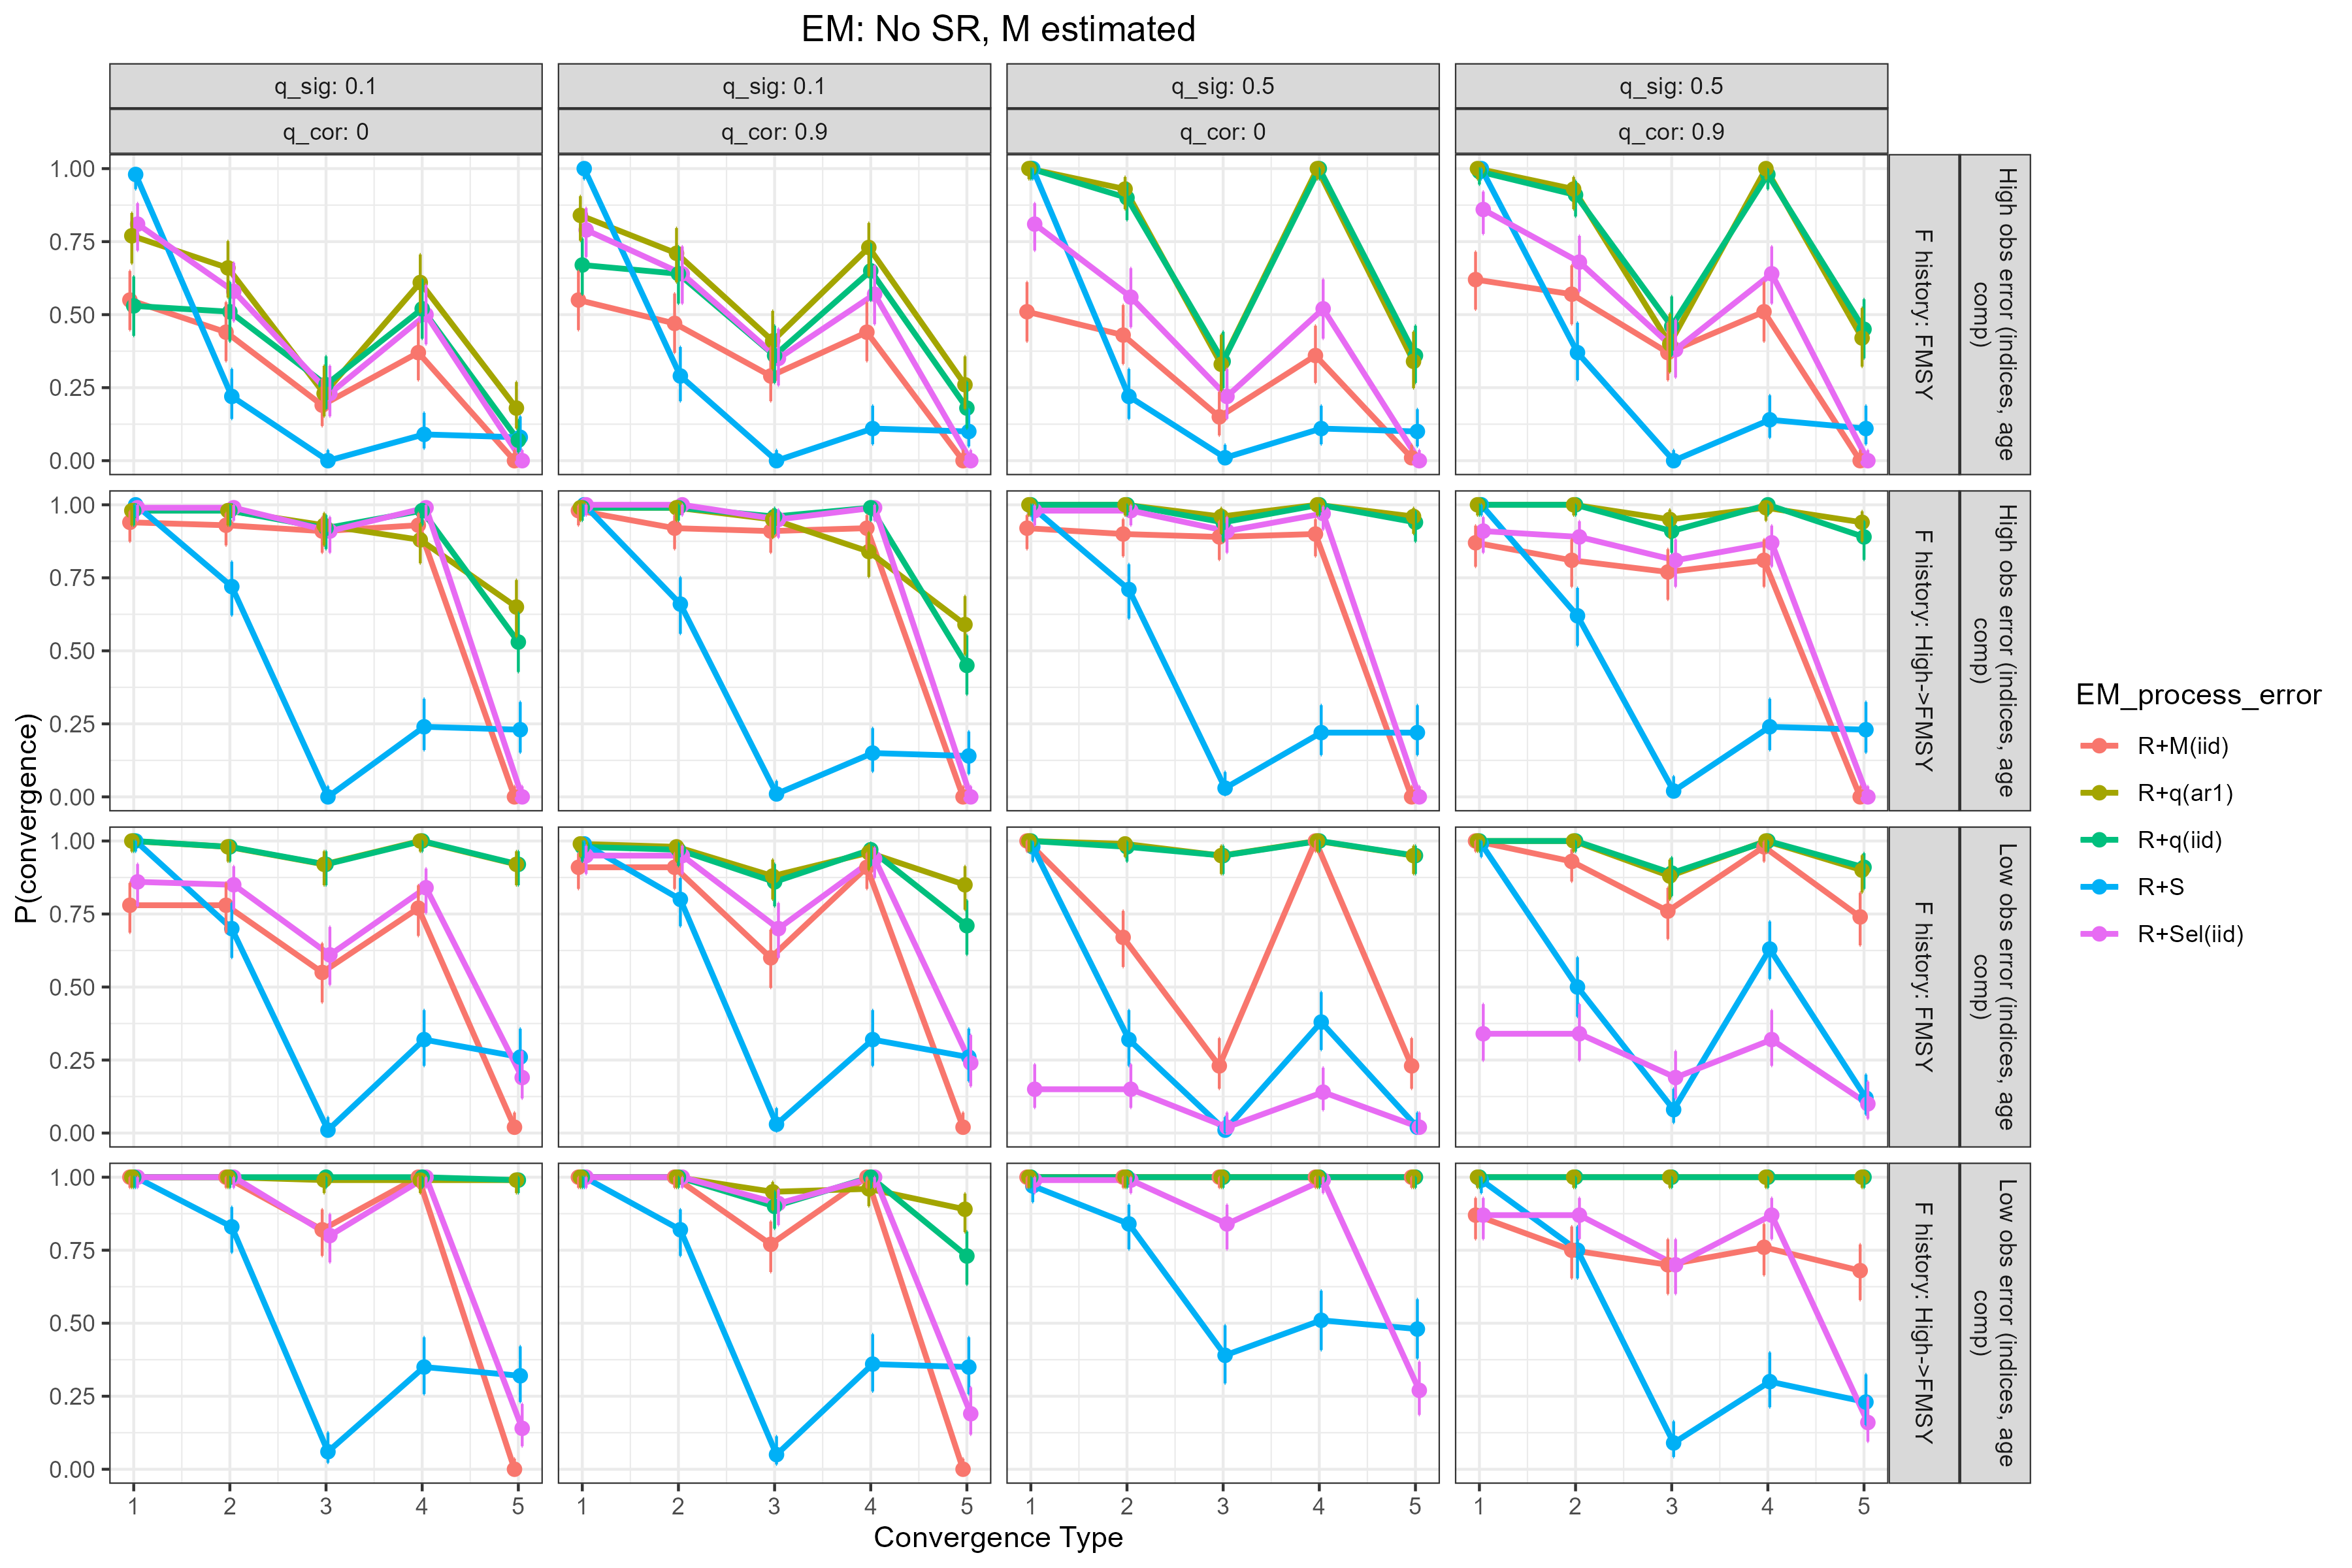
\includegraphics[width = \textwidth]{q_om_p_convergence_meanR_M_estimated.png}
\end{center}
\end{figure}
\end{landscape}

\begin{landscape}
\begin{figure}
\caption{Probability of each type of convergence of estimating models with alternative process error assumptions for operating models that have process error structure R+q. vertical lines represent 95\% confidence intervals. All estimating models estimate a Beverton-Holt stock-recruit relationship and and M is fixed at the true value.}\label{q_om_em_BH_MF_convergence}
\begin{center}
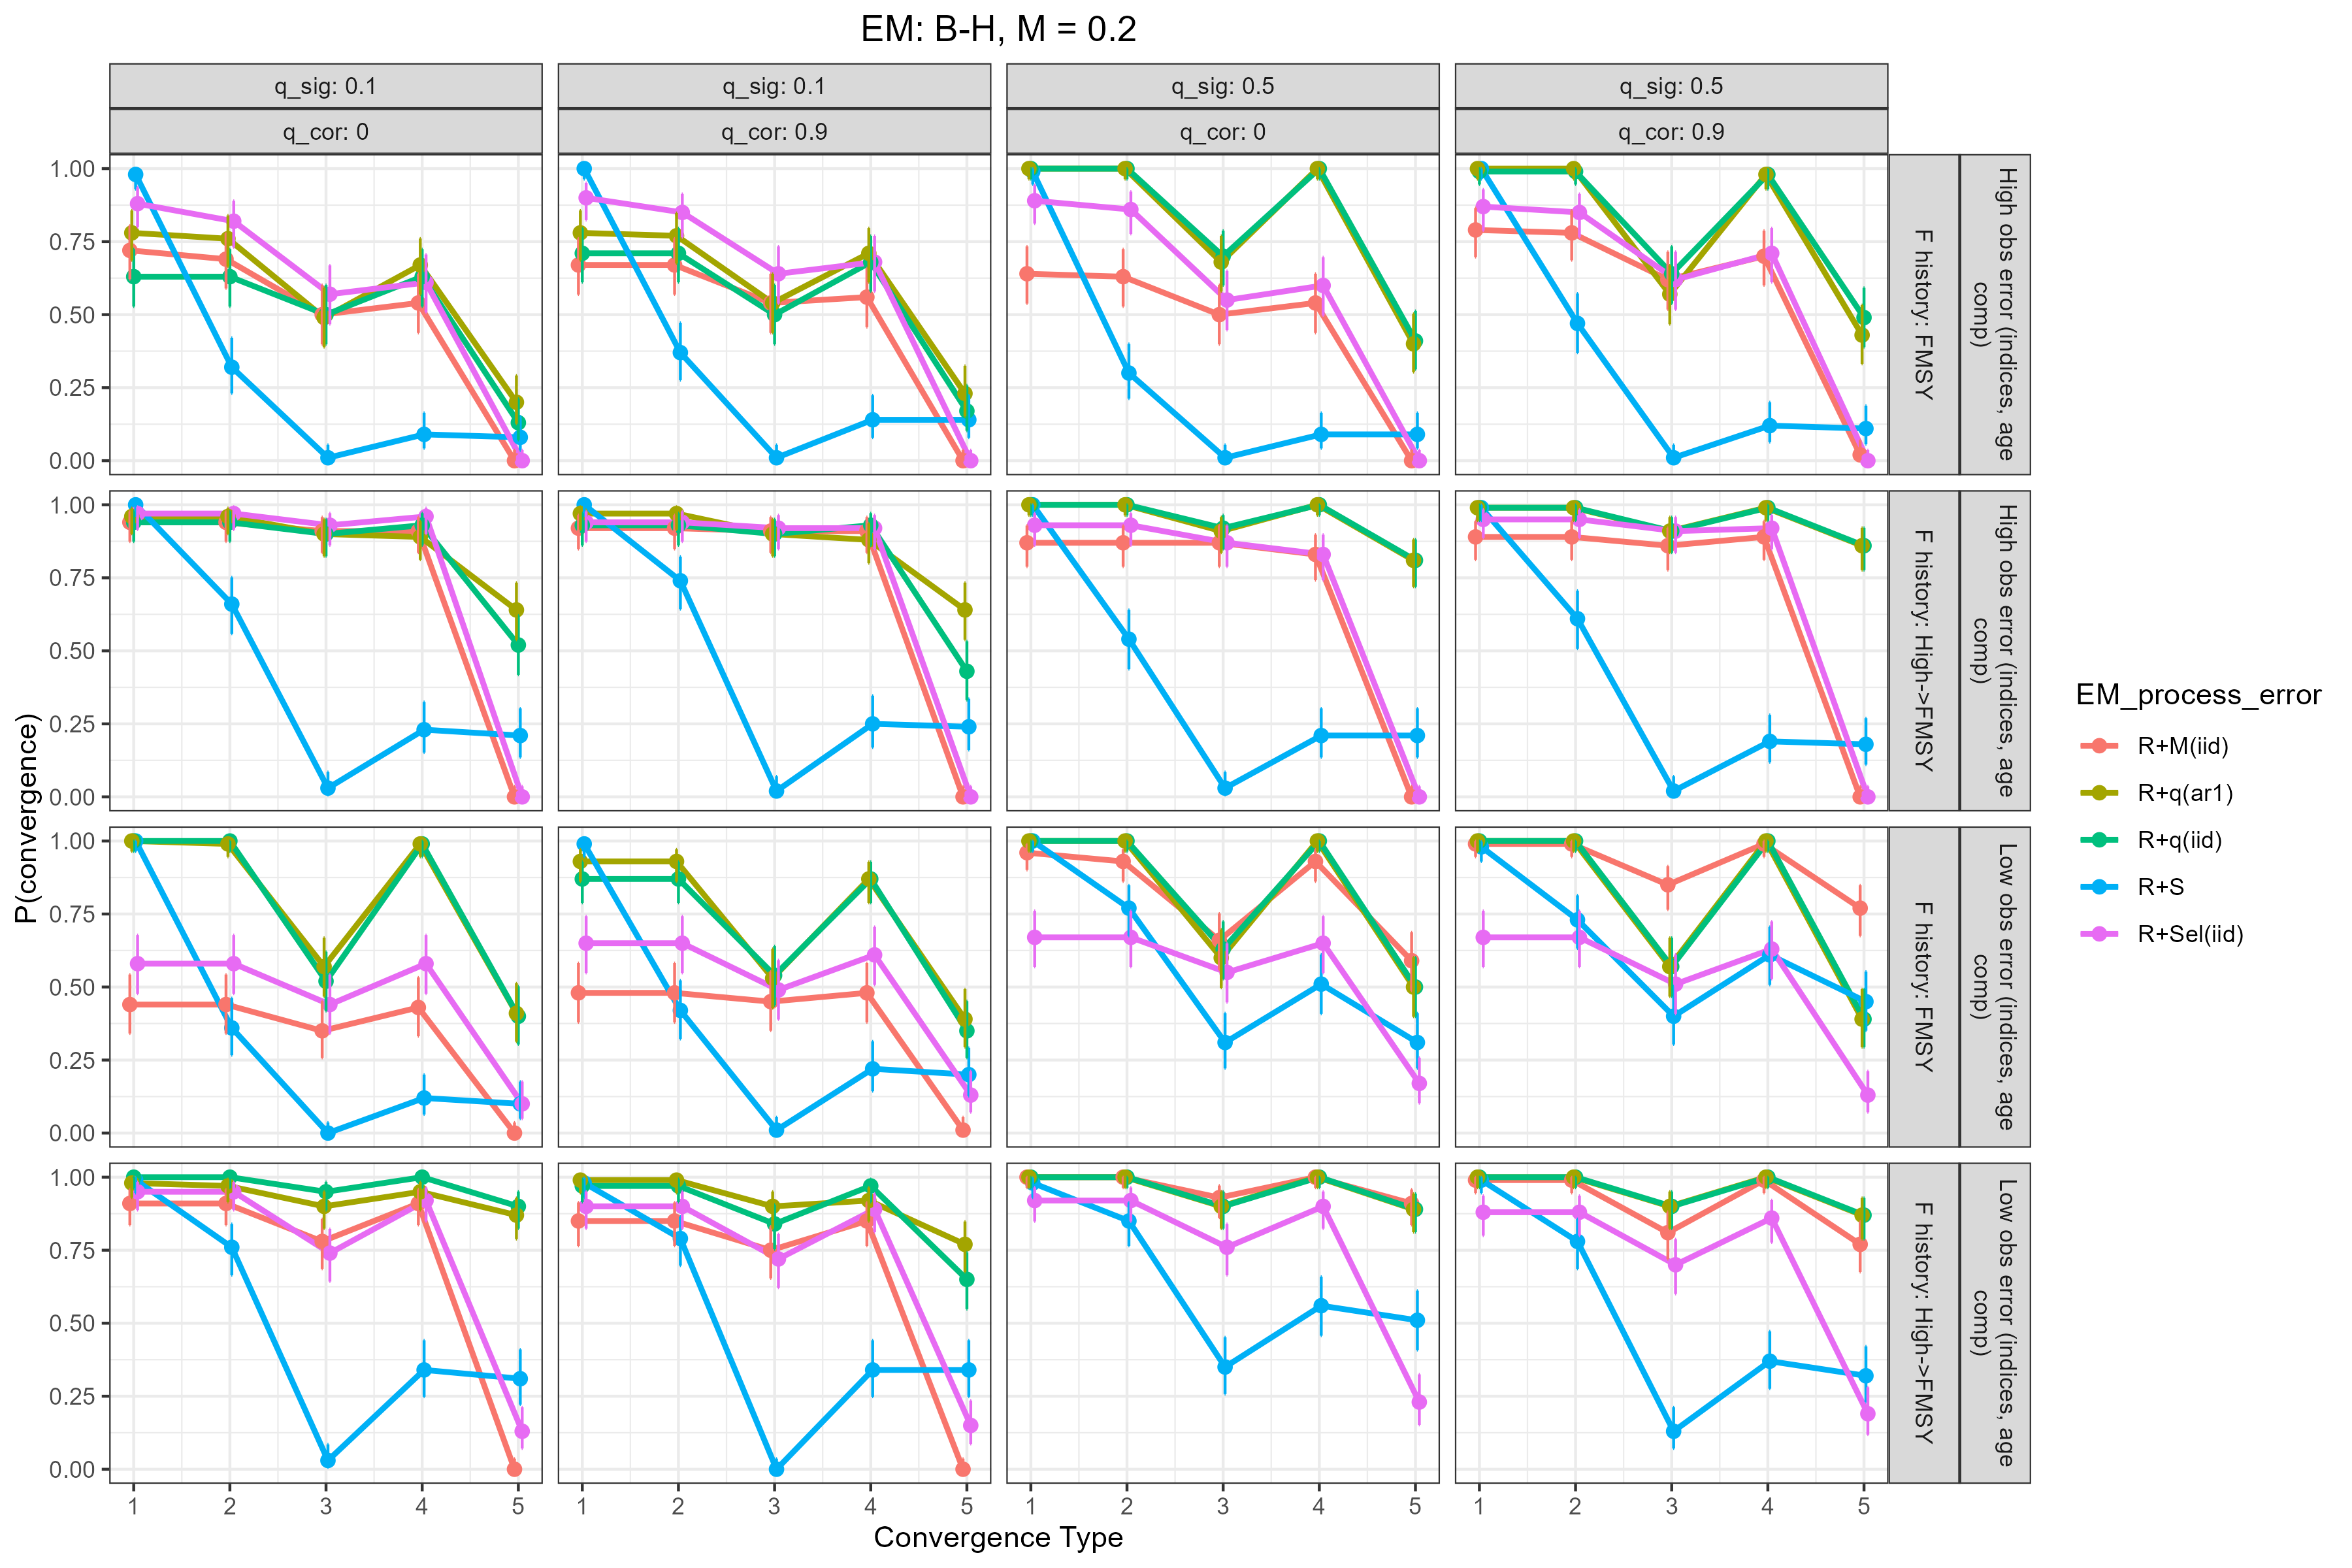
\includegraphics[width = \textwidth]{q_om_p_convergence_BH_M_fixed.png}
\end{center}
\end{figure}
\end{landscape}

\begin{landscape}
\begin{figure}
\caption{Probability of each type of convergence of estimating models with alternative process error assumptions for operating models that have process error structure R+q. vertical lines represent 95\% confidence intervals. All estimating models estimate a Beverton-Holt stock-recruit relationship and and M is estimated.}\label{q_om_em_BH_ME_convergence}
\begin{center}
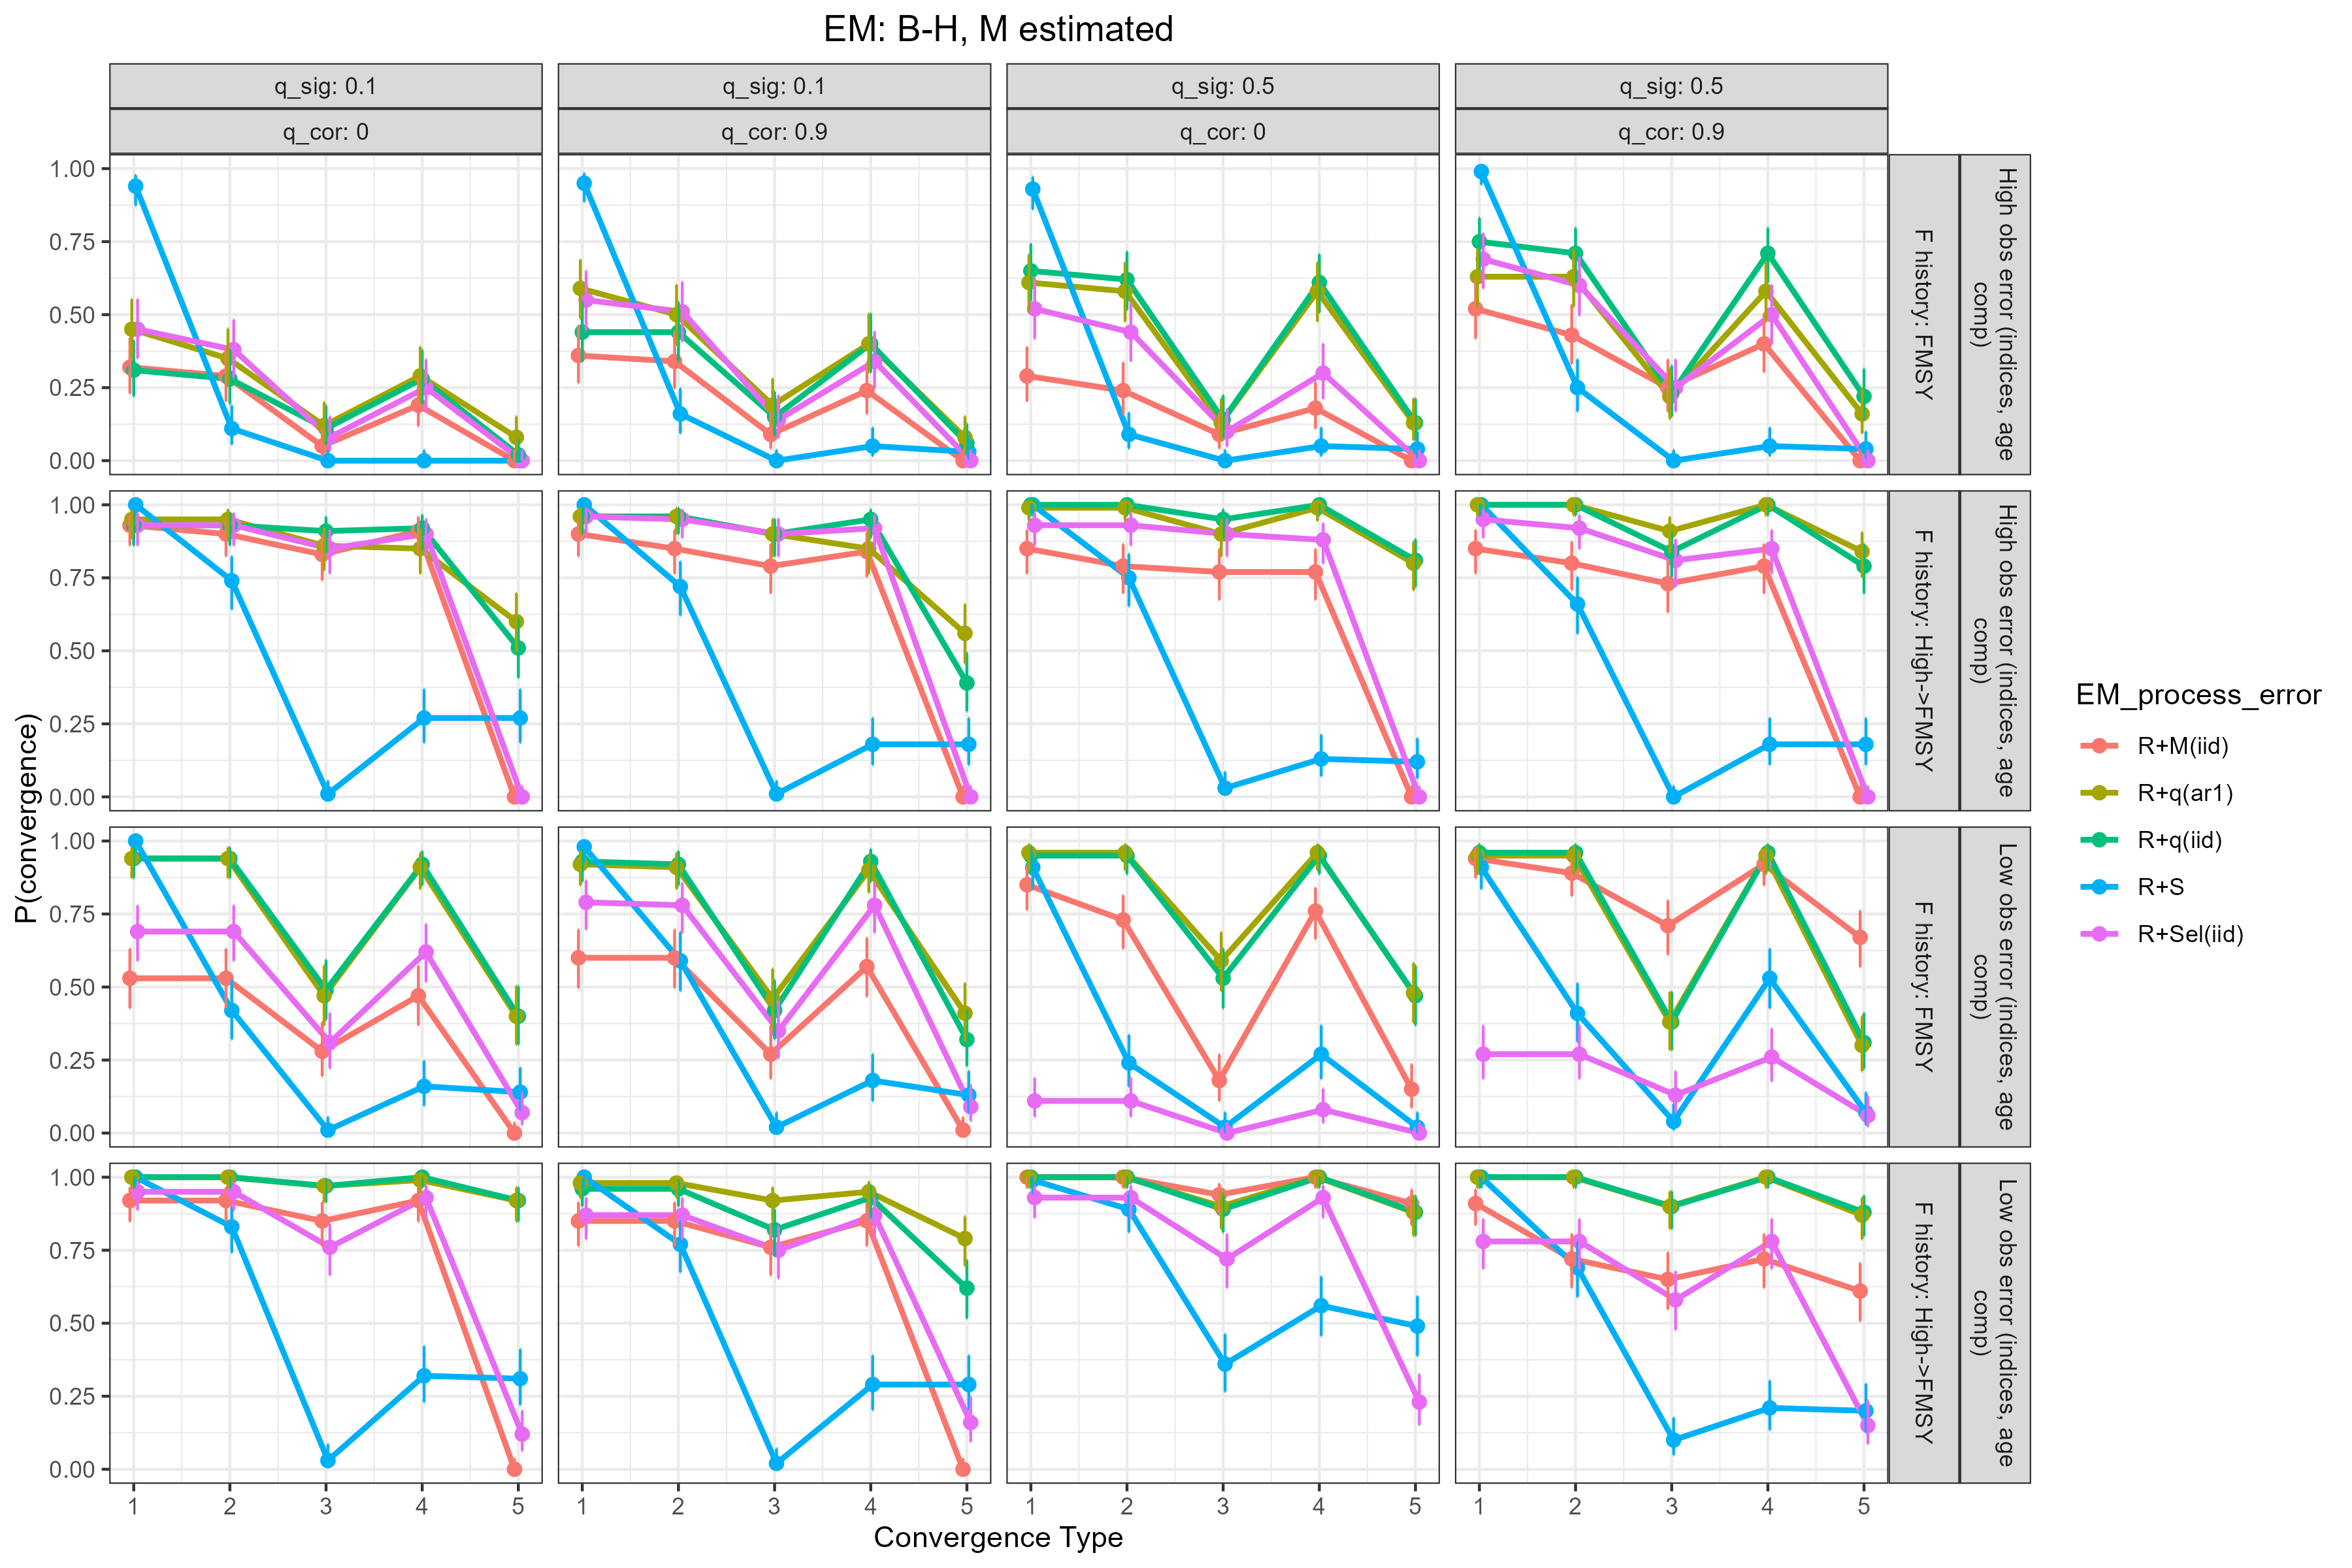
\includegraphics[width = \textwidth]{q_om_p_convergence_BH_M_estimated.png}
\end{center}
\end{figure}
\end{landscape}

\begin{landscape}
\begin{figure}
\caption{Proportion of simulated data sets from OMs with R and R+S process errors where fitted estimating models had lowest marginal AIC. All estimating models estimate mean recruitment rather than a stock-recruit relationship and and M is fixed at the true value.} \label{naa_om_proportion_best_aic_R_MF}
\begin{center}
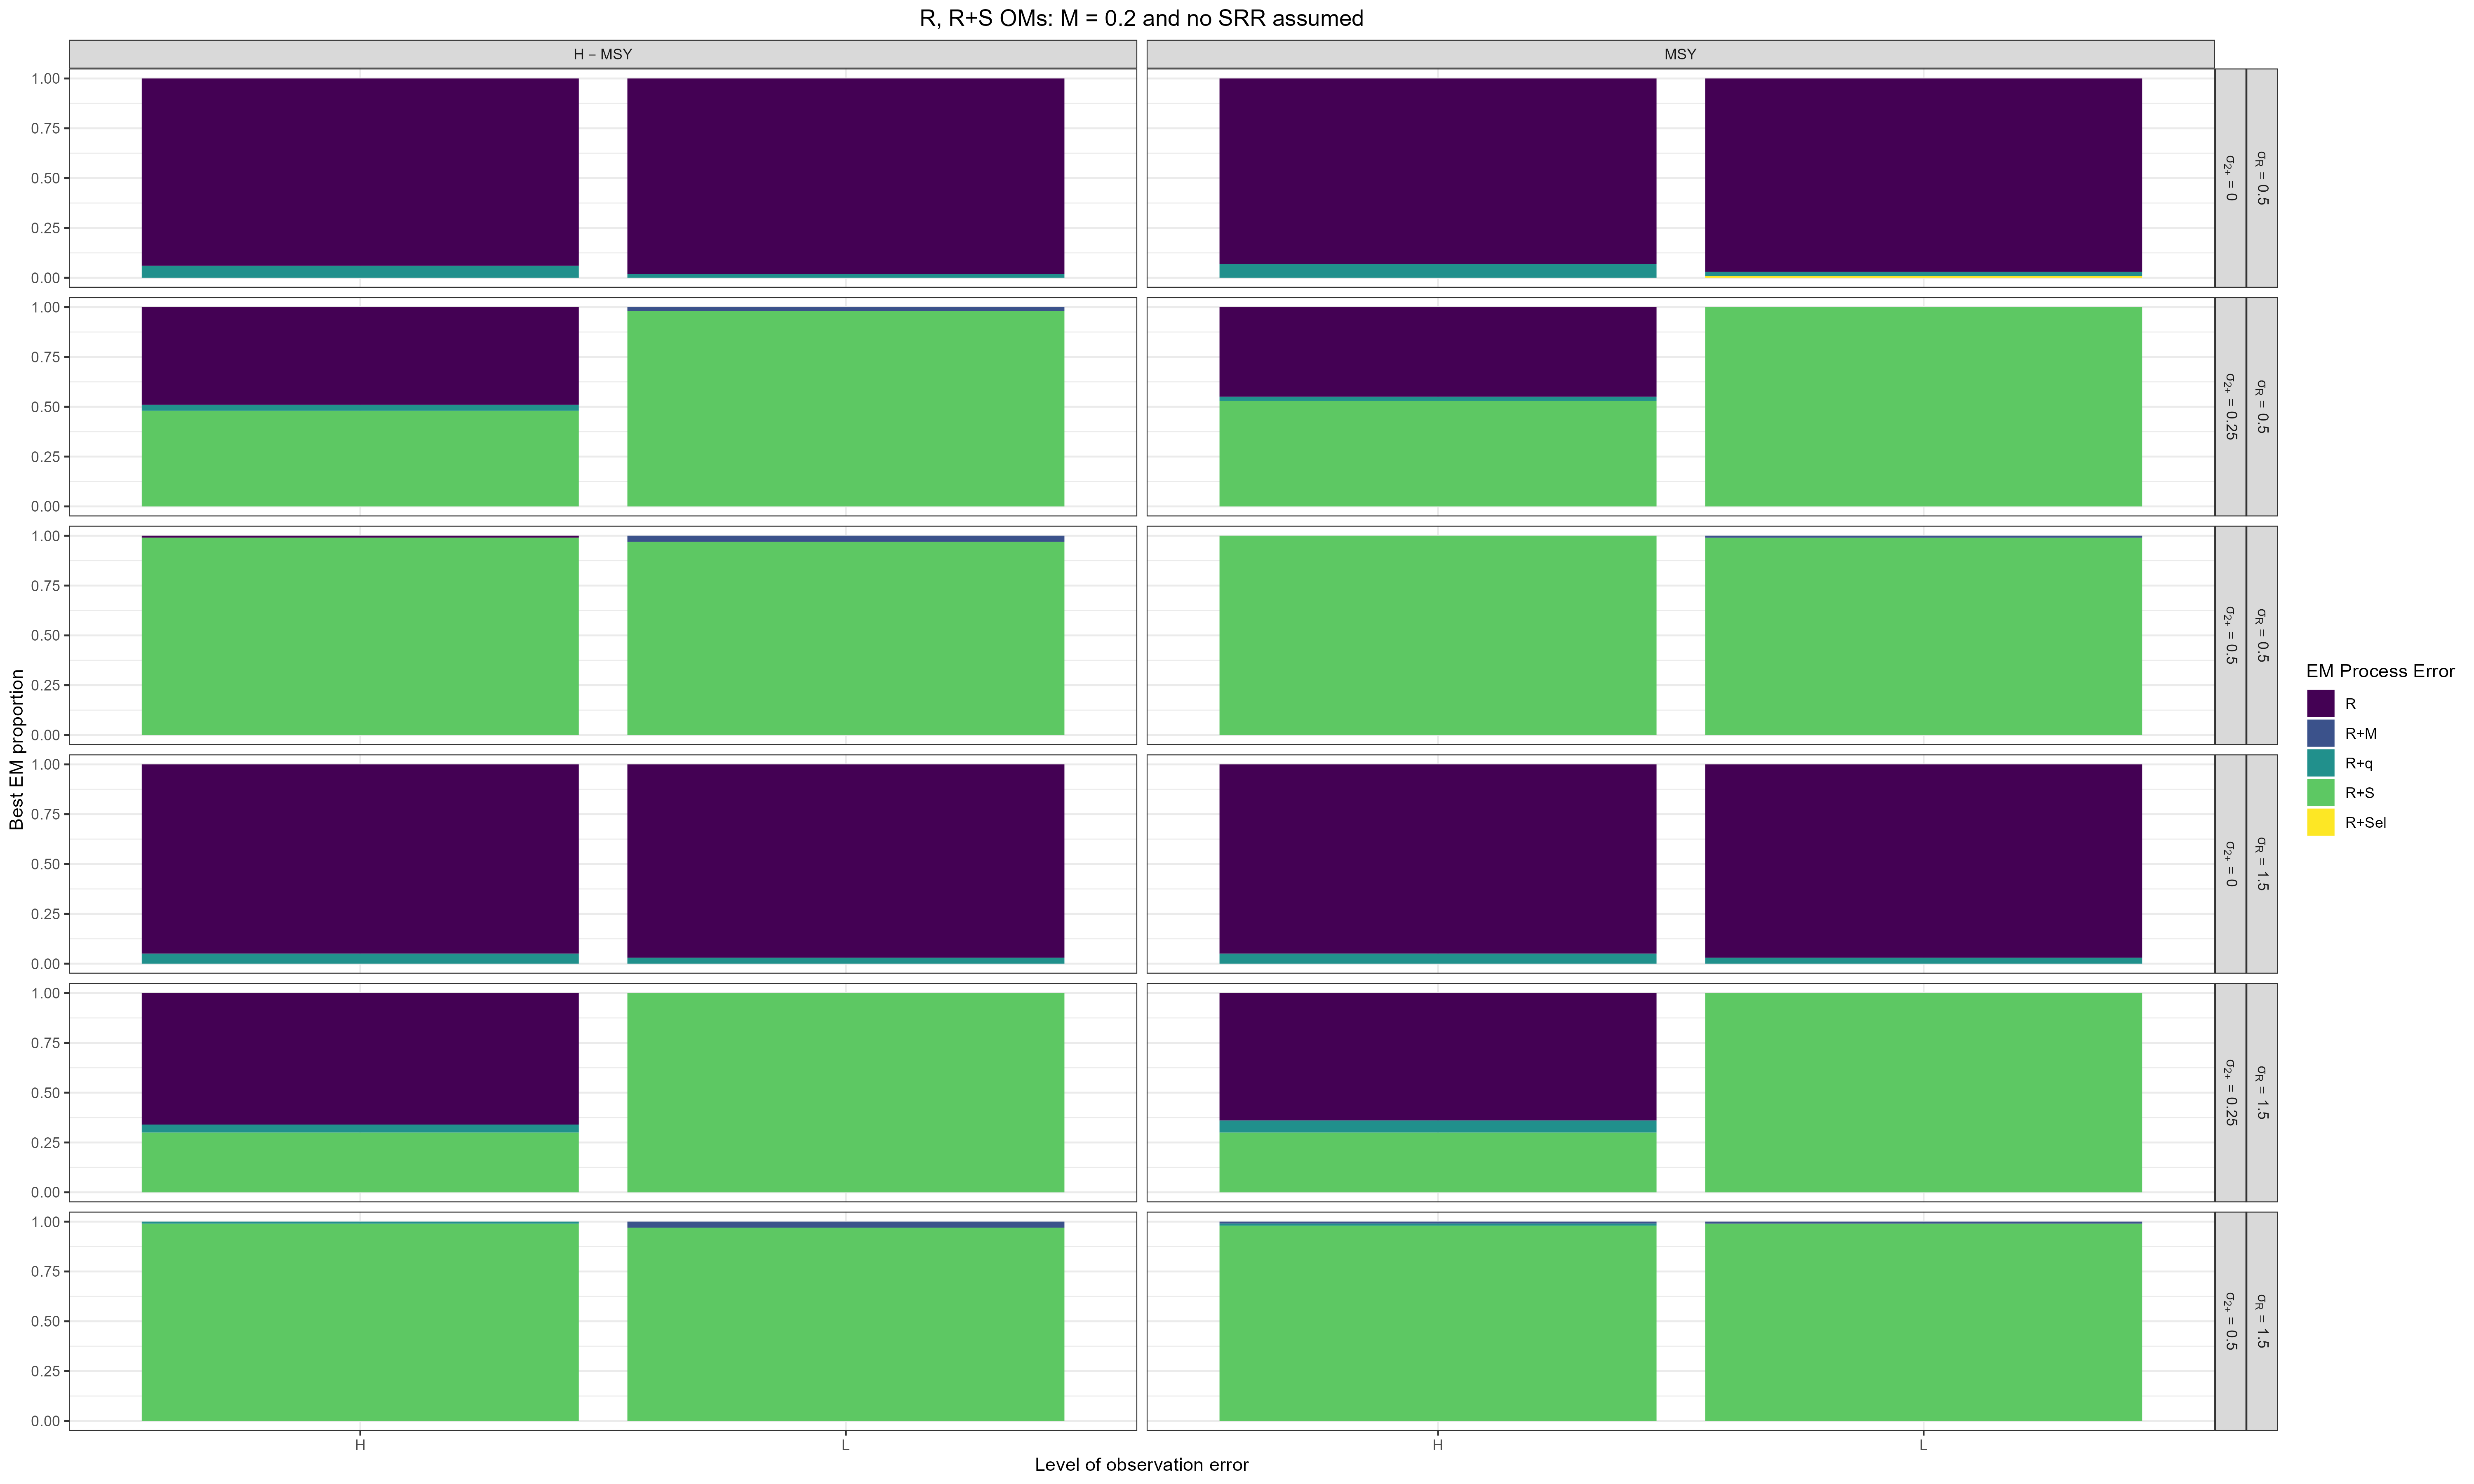
\includegraphics[width = \textwidth]{naa_om_proportion_best_aic_R_MF.png}
\end{center}
\end{figure}
\end{landscape}

\begin{landscape}
\begin{figure}
\caption{Proportion of simulated data sets from OMs with R and R+S process errors where fitted estimating models had lowest marginal AIC. All estimating models estimate mean recruitment rather than a stock-recruit relationship and and M is estimated.} \label{naa_om_proportion_best_aic_R_ME}
\begin{center}
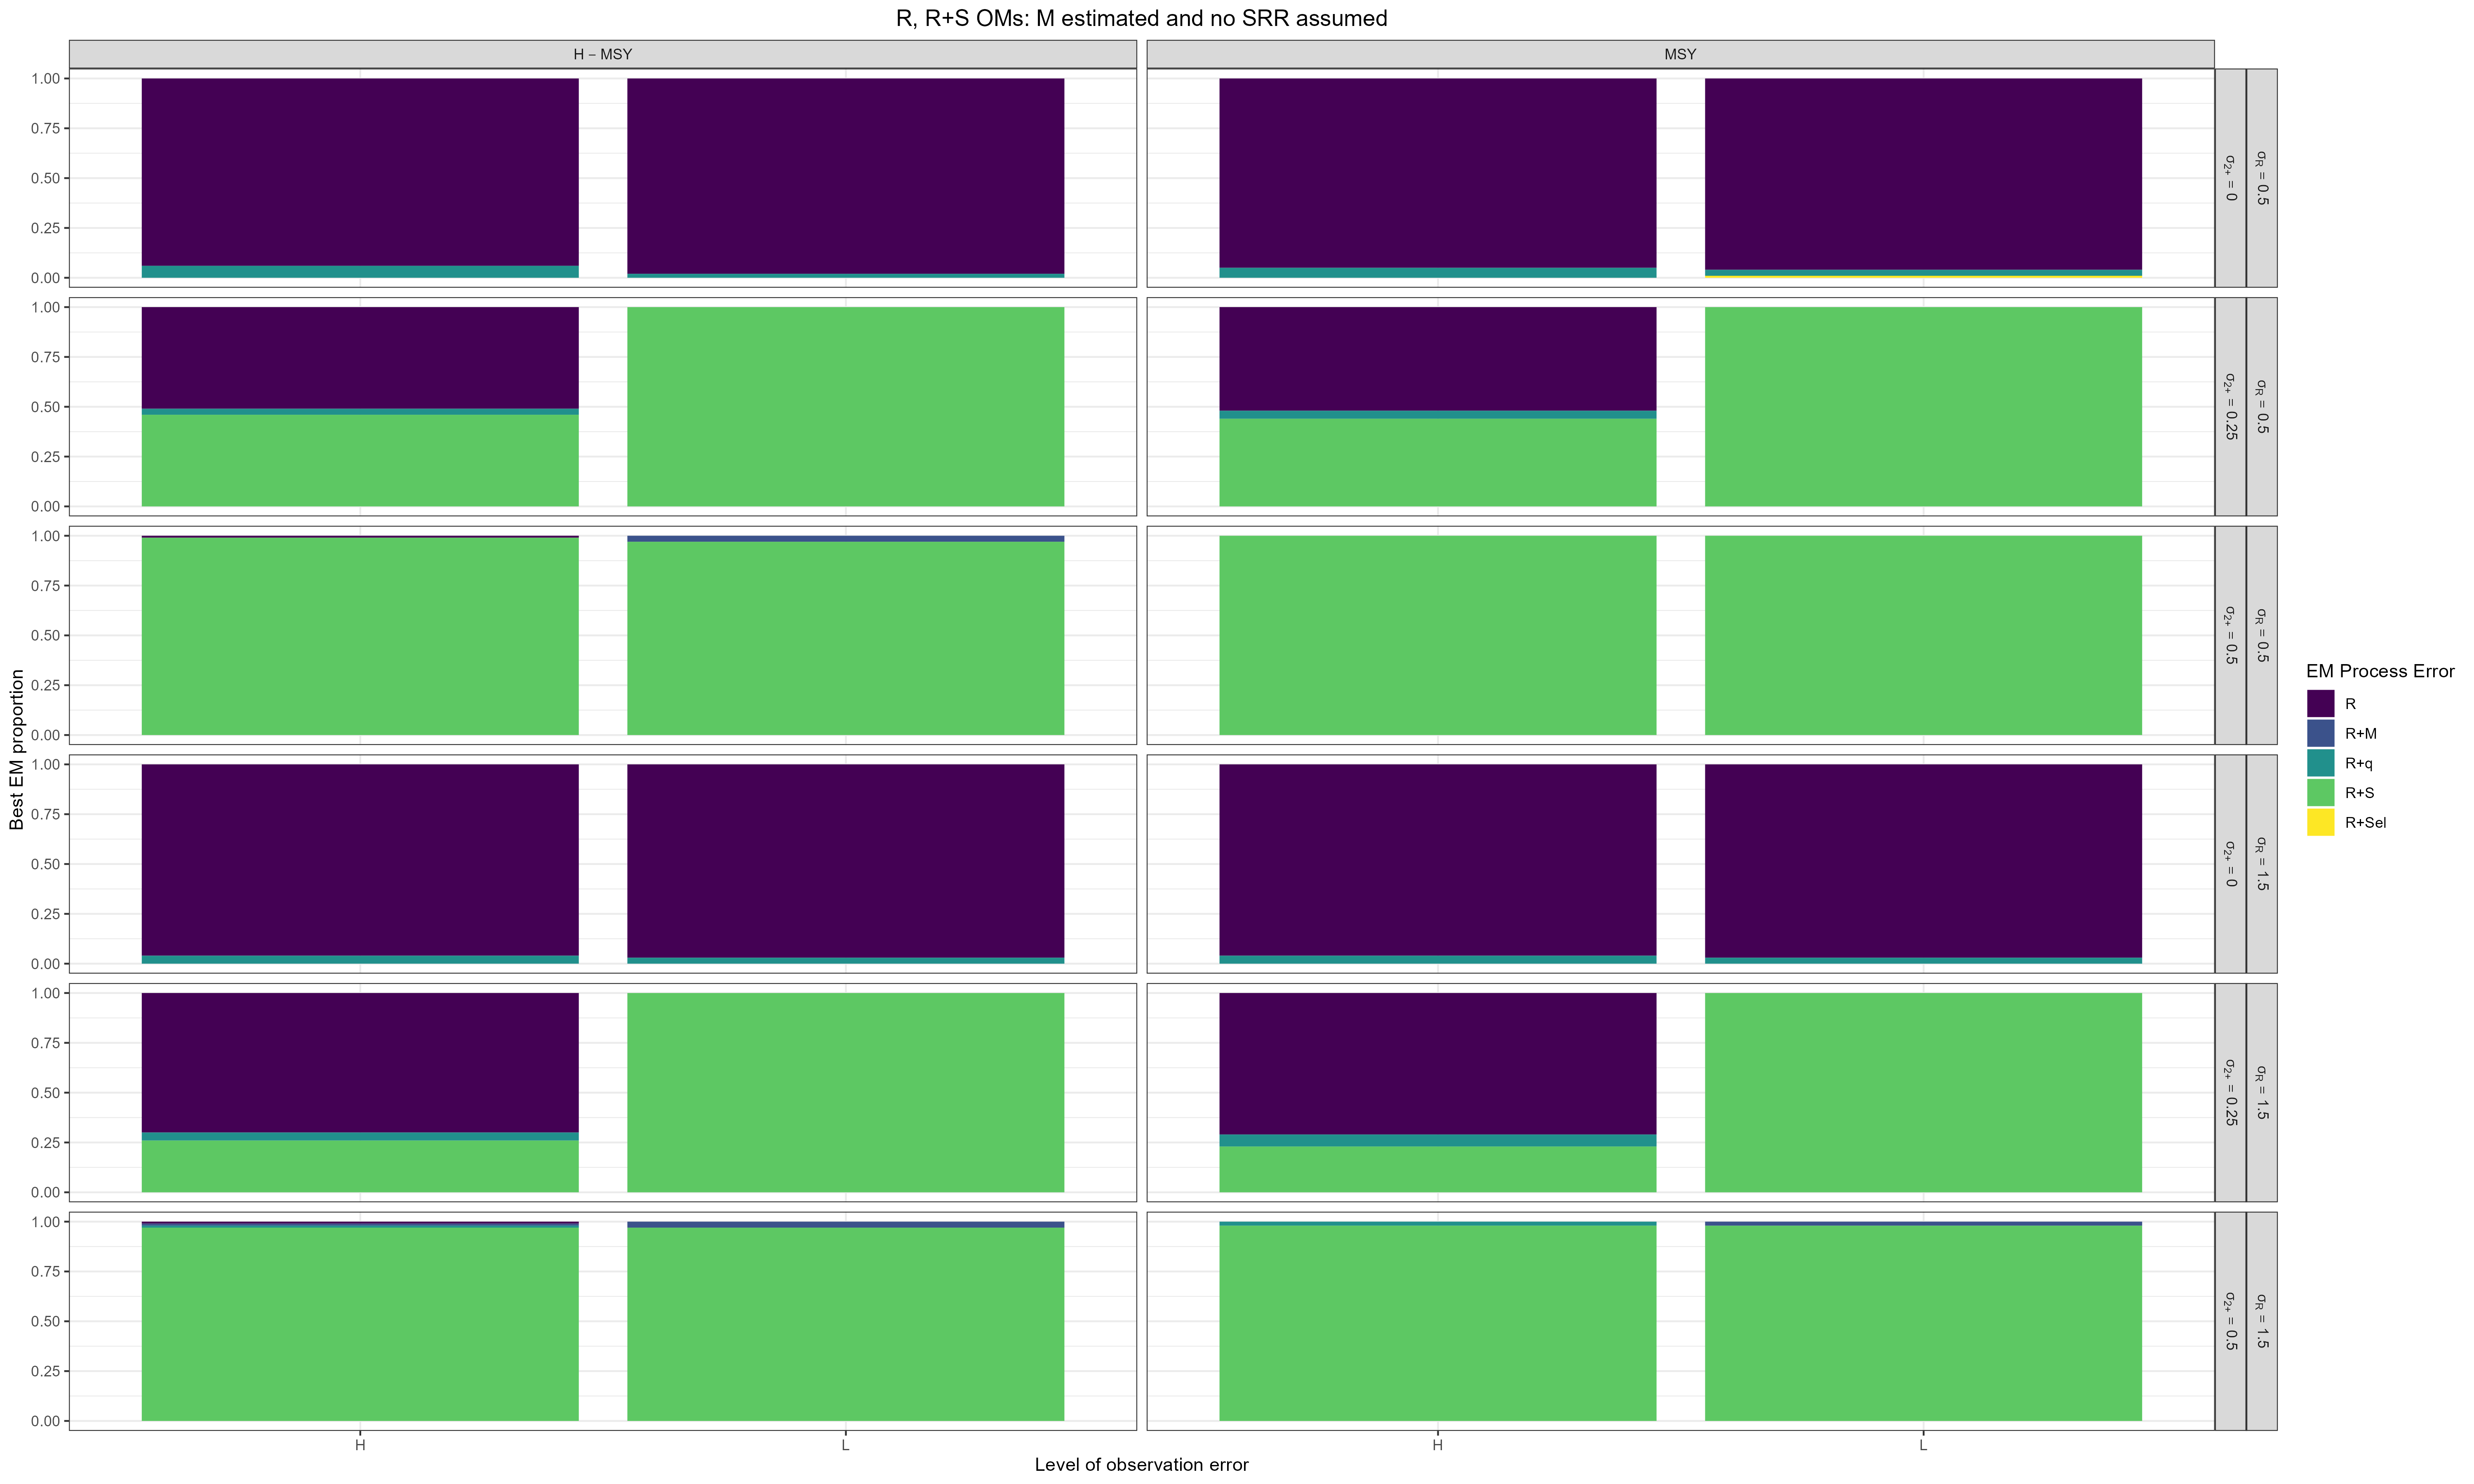
\includegraphics[width = \textwidth]{naa_om_proportion_best_aic_R_ME.png}
\end{center}
\end{figure}
\end{landscape}

\begin{landscape}
\begin{figure}
\caption{Proportion of simulated data sets from OMs with R and R+S process errors where fitted estimating models had lowest marginal AIC. All estimating models estimate a stock-recruit relationship and and M is fixed at the true value.} \label{naa_om_proportion_best_aic_SR_MF}
\begin{center}
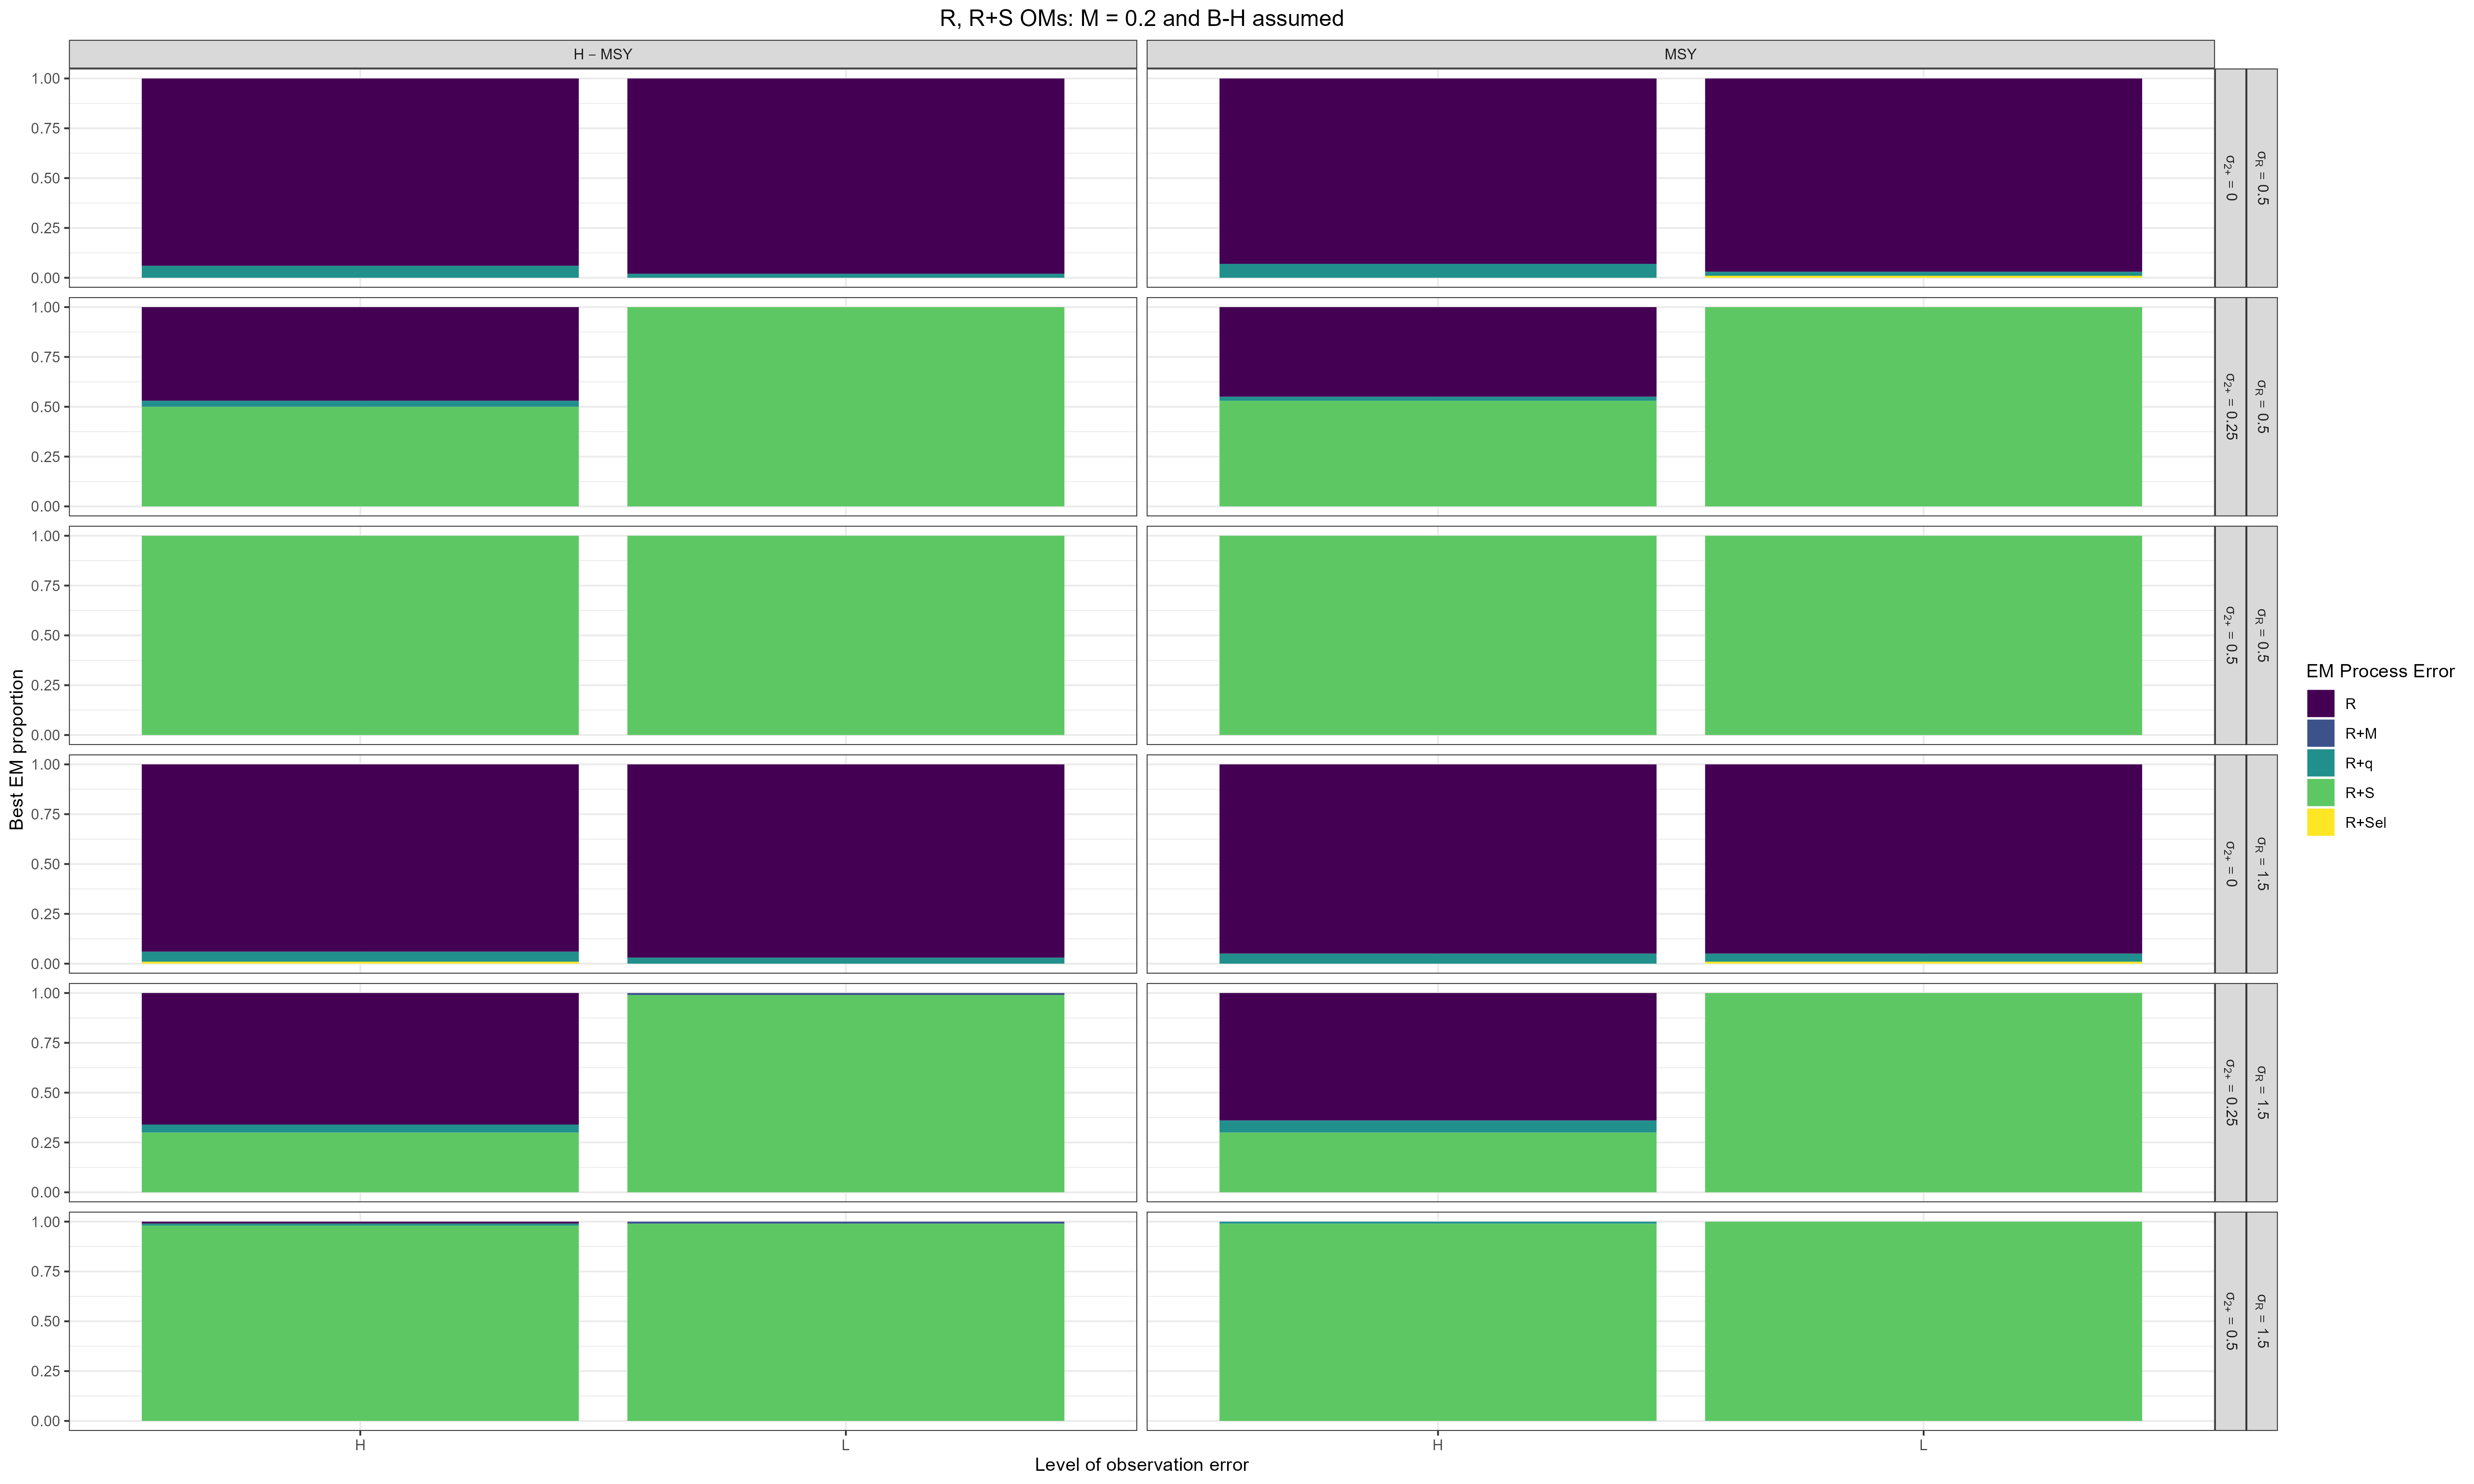
\includegraphics[width = \textwidth]{naa_om_proportion_best_aic_SR_MF.png}
\end{center}
\end{figure}
\end{landscape}

\begin{landscape}
\begin{figure}
\caption{Proportion of simulated data sets from OMs with R and R+S process errors where fitted estimating models had lowest marginal AIC. All estimating models estimate a stock-recruit relationship and and M is estimated.} \label{naa_om_proportion_best_aic_SR_ME}
\begin{center}
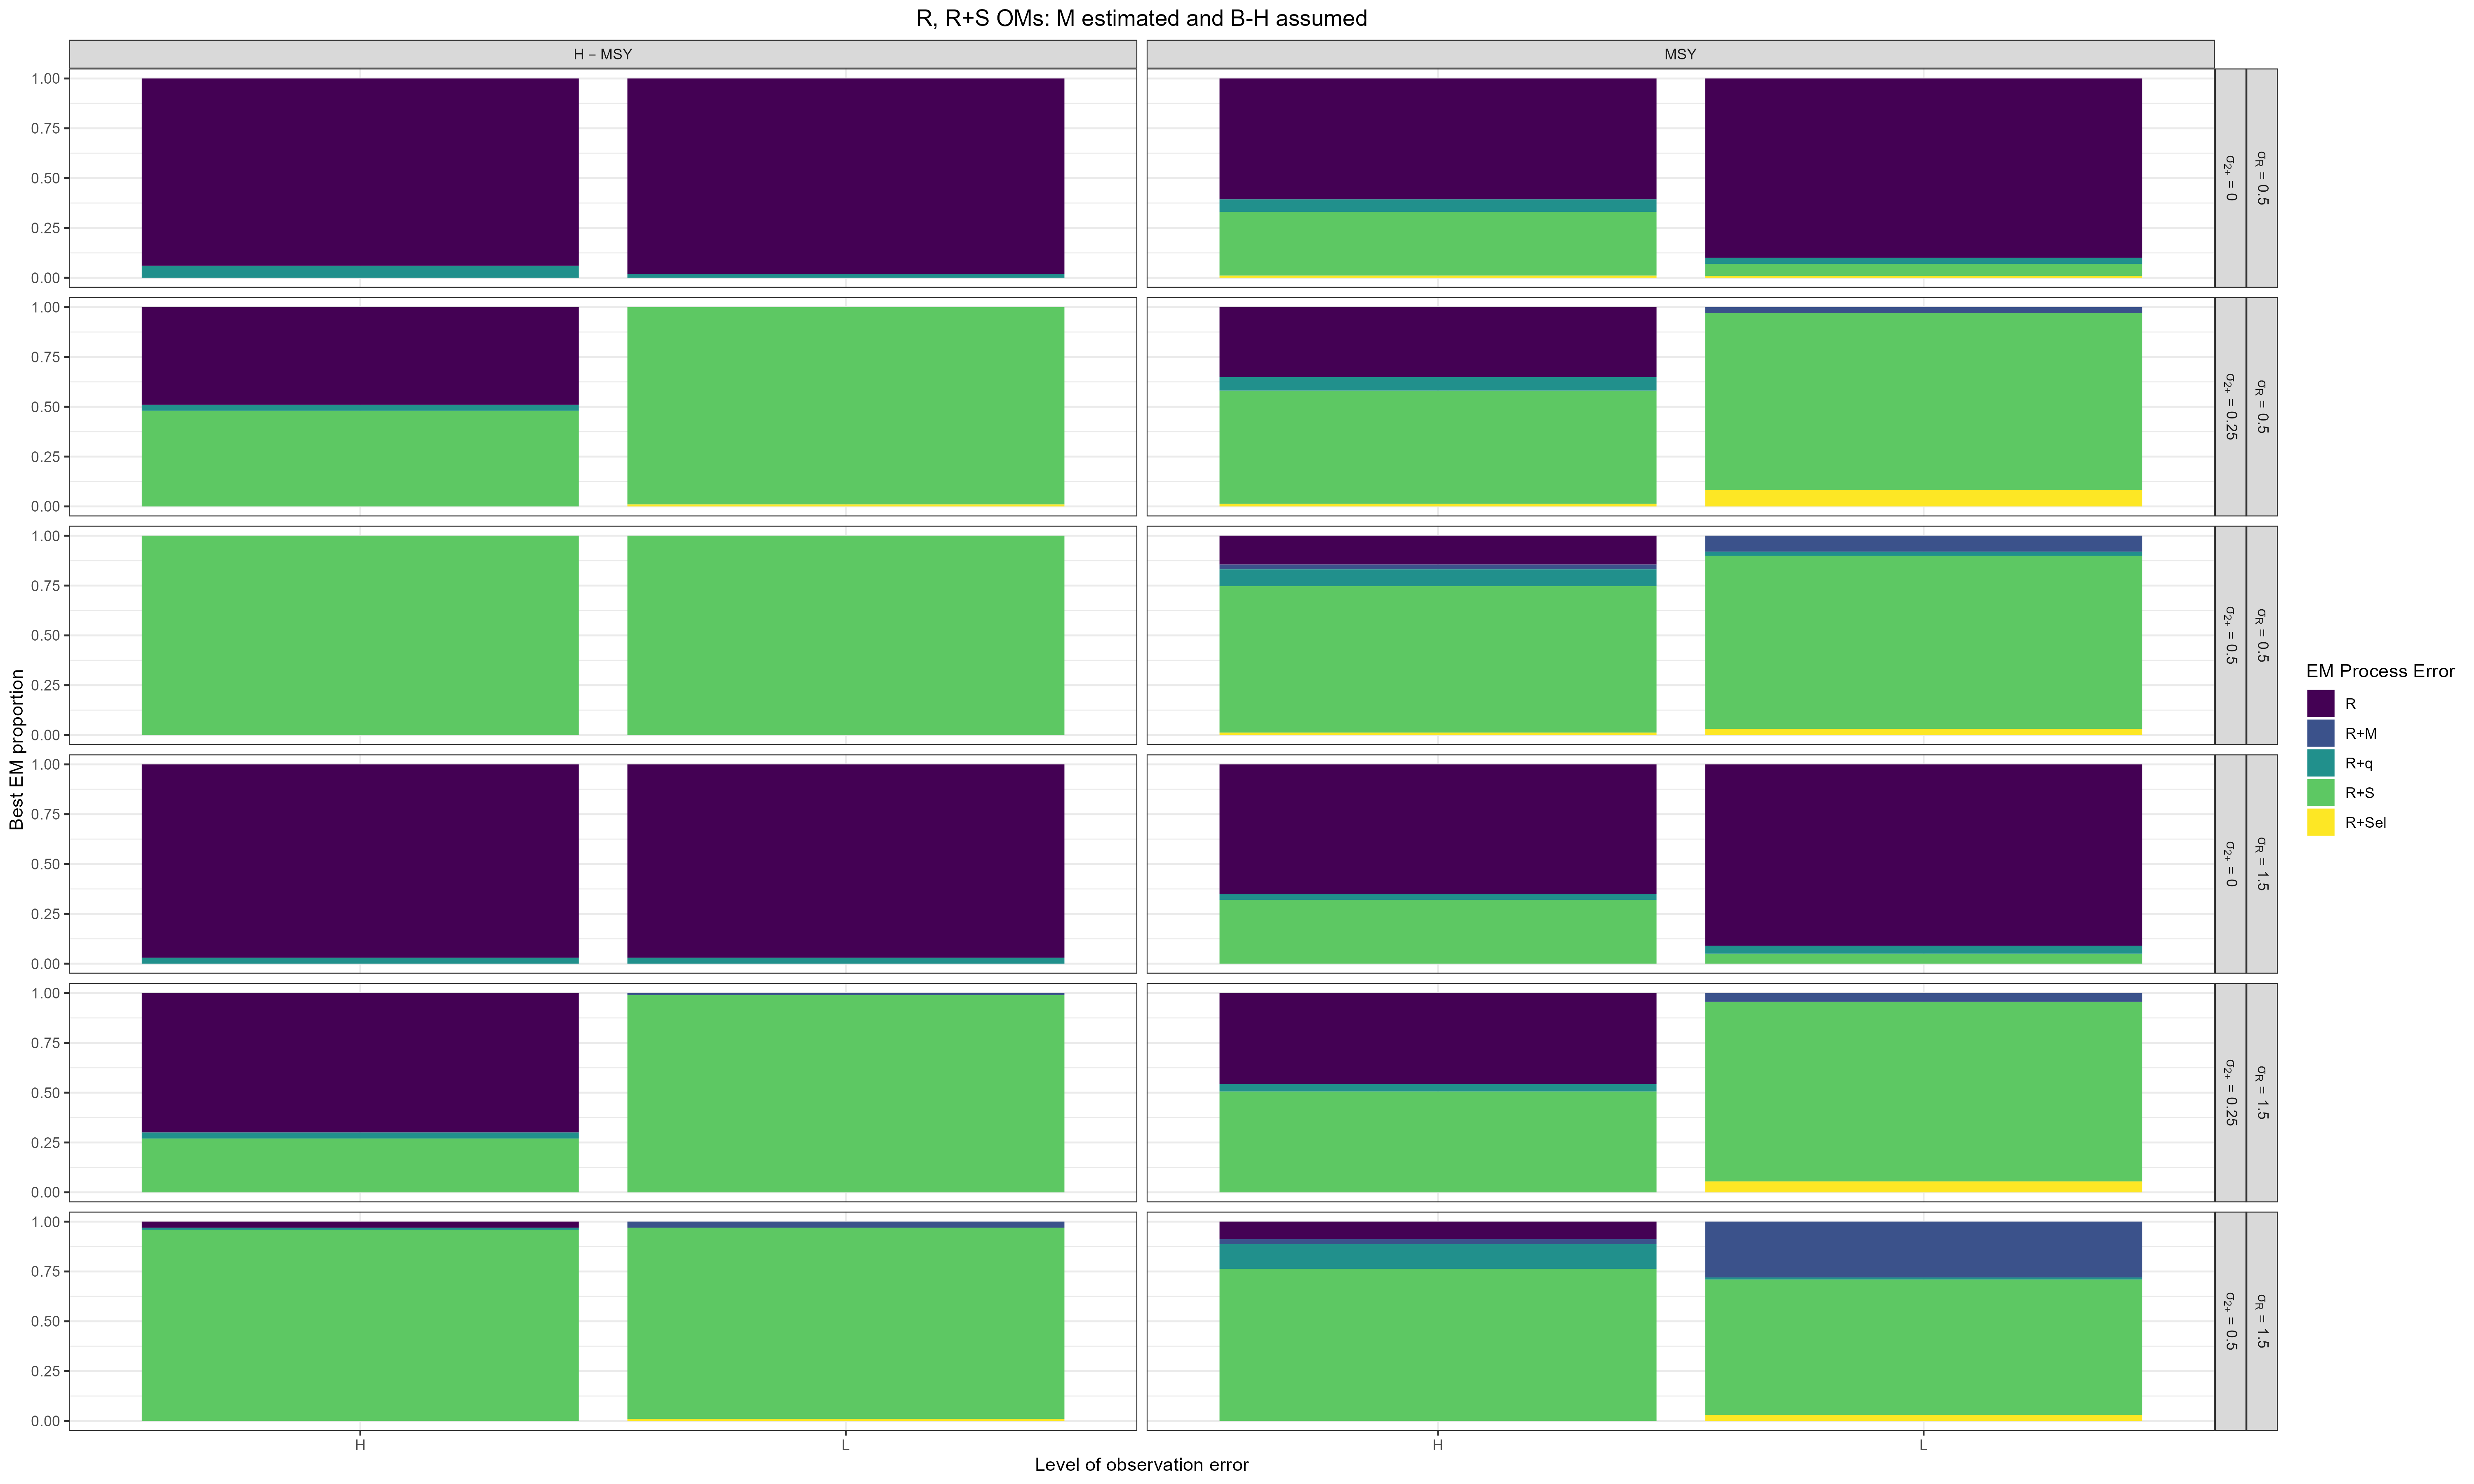
\includegraphics[width = \textwidth]{naa_om_proportion_best_aic_SR_ME.png}
\end{center}
\end{figure}
\end{landscape}

\begin{landscape}
\begin{figure}
\caption{Proportion of simulated data sets from OMs with R+M process errors where fitted estimating models had lowest marginal AIC. All estimating models estimate mean recruitment rather than a stock-recruit relationship and and M is fixed at the true value.} \label{M_om_proportion_best_aic_R_MF}
\begin{center}
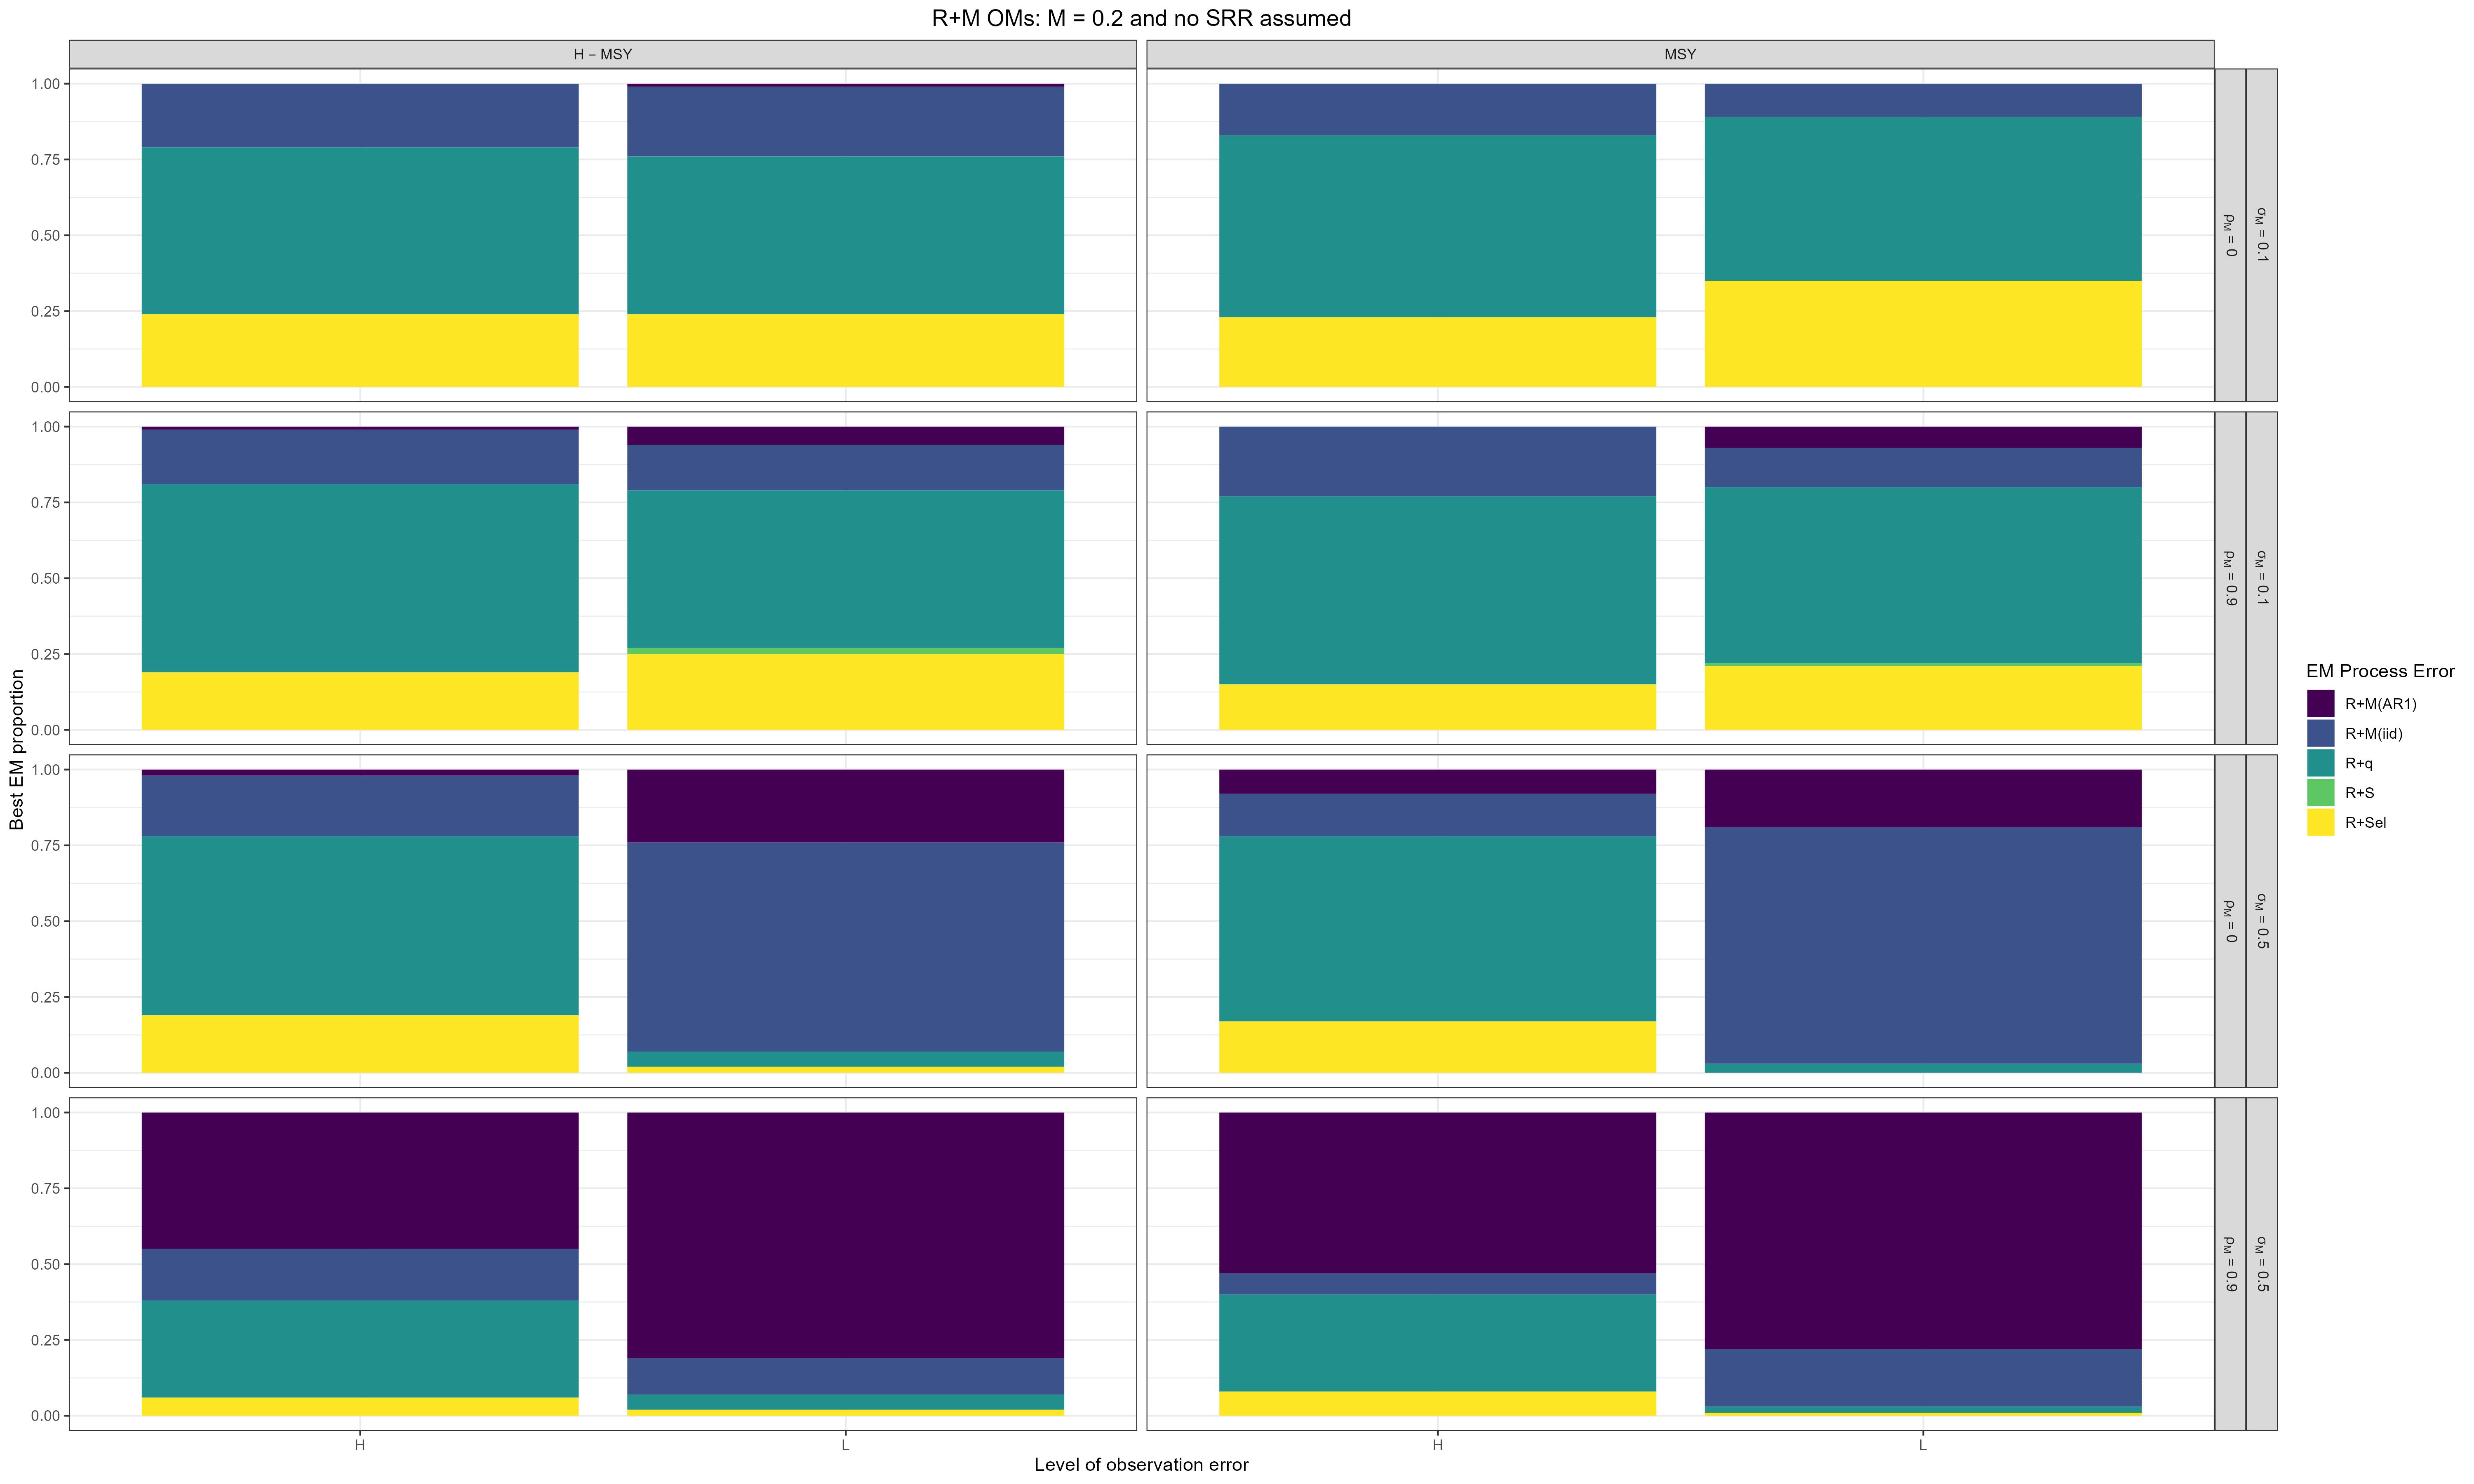
\includegraphics[width = \textwidth]{M_om_proportion_best_aic_R_MF.png}
\end{center}
\end{figure}
\end{landscape}

\begin{landscape}
\begin{figure}
\caption{Proportion of simulated data sets from OMs with R+M process errors where fitted estimating models had lowest marginal AIC. All estimating models estimate mean recruitment rather than a stock-recruit relationship and and M is estimated.} \label{M_om_proportion_best_aic_R_ME}
\begin{center}
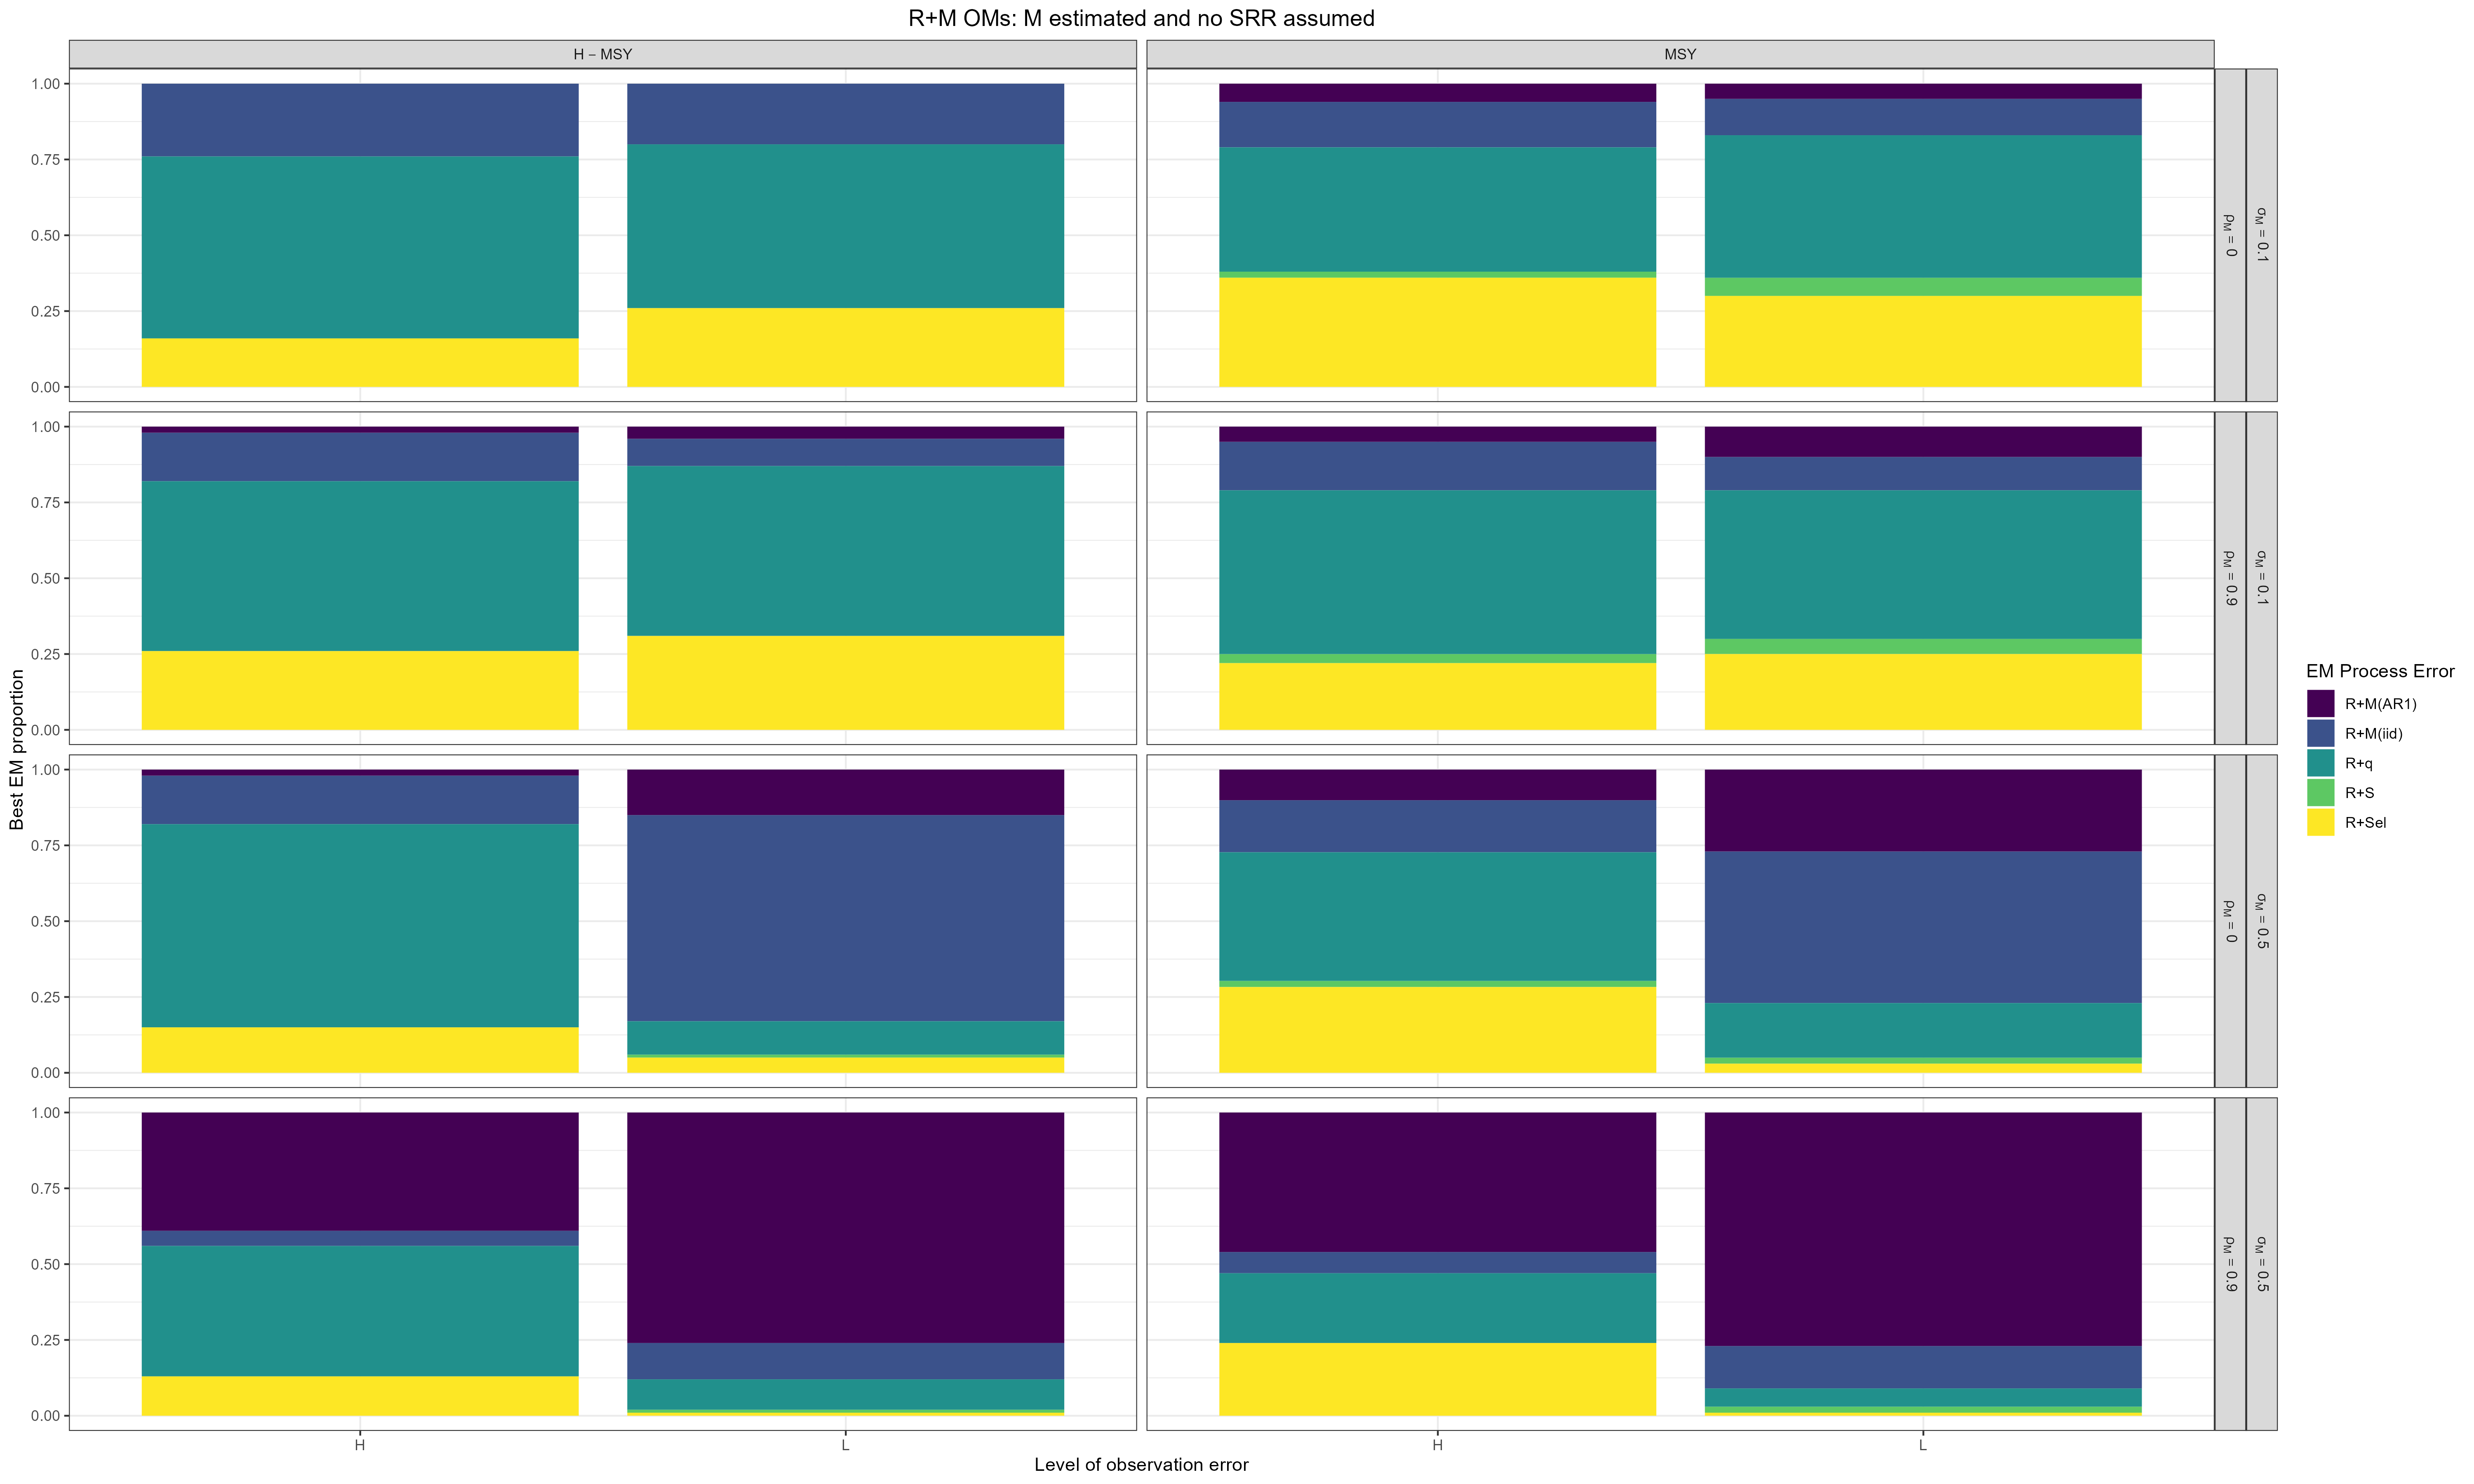
\includegraphics[width = \textwidth]{M_om_proportion_best_aic_R_ME.png}
\end{center}
\end{figure}
\end{landscape}

\begin{landscape}
\begin{figure}
\caption{Proportion of simulated data sets from OMs with R+M process errors where fitted estimating models had lowest marginal AIC. All estimating models estimate a stock-recruit relationship and and M is fixed at the true value.} \label{M_om_proportion_best_aic_SR_MF}
\begin{center}
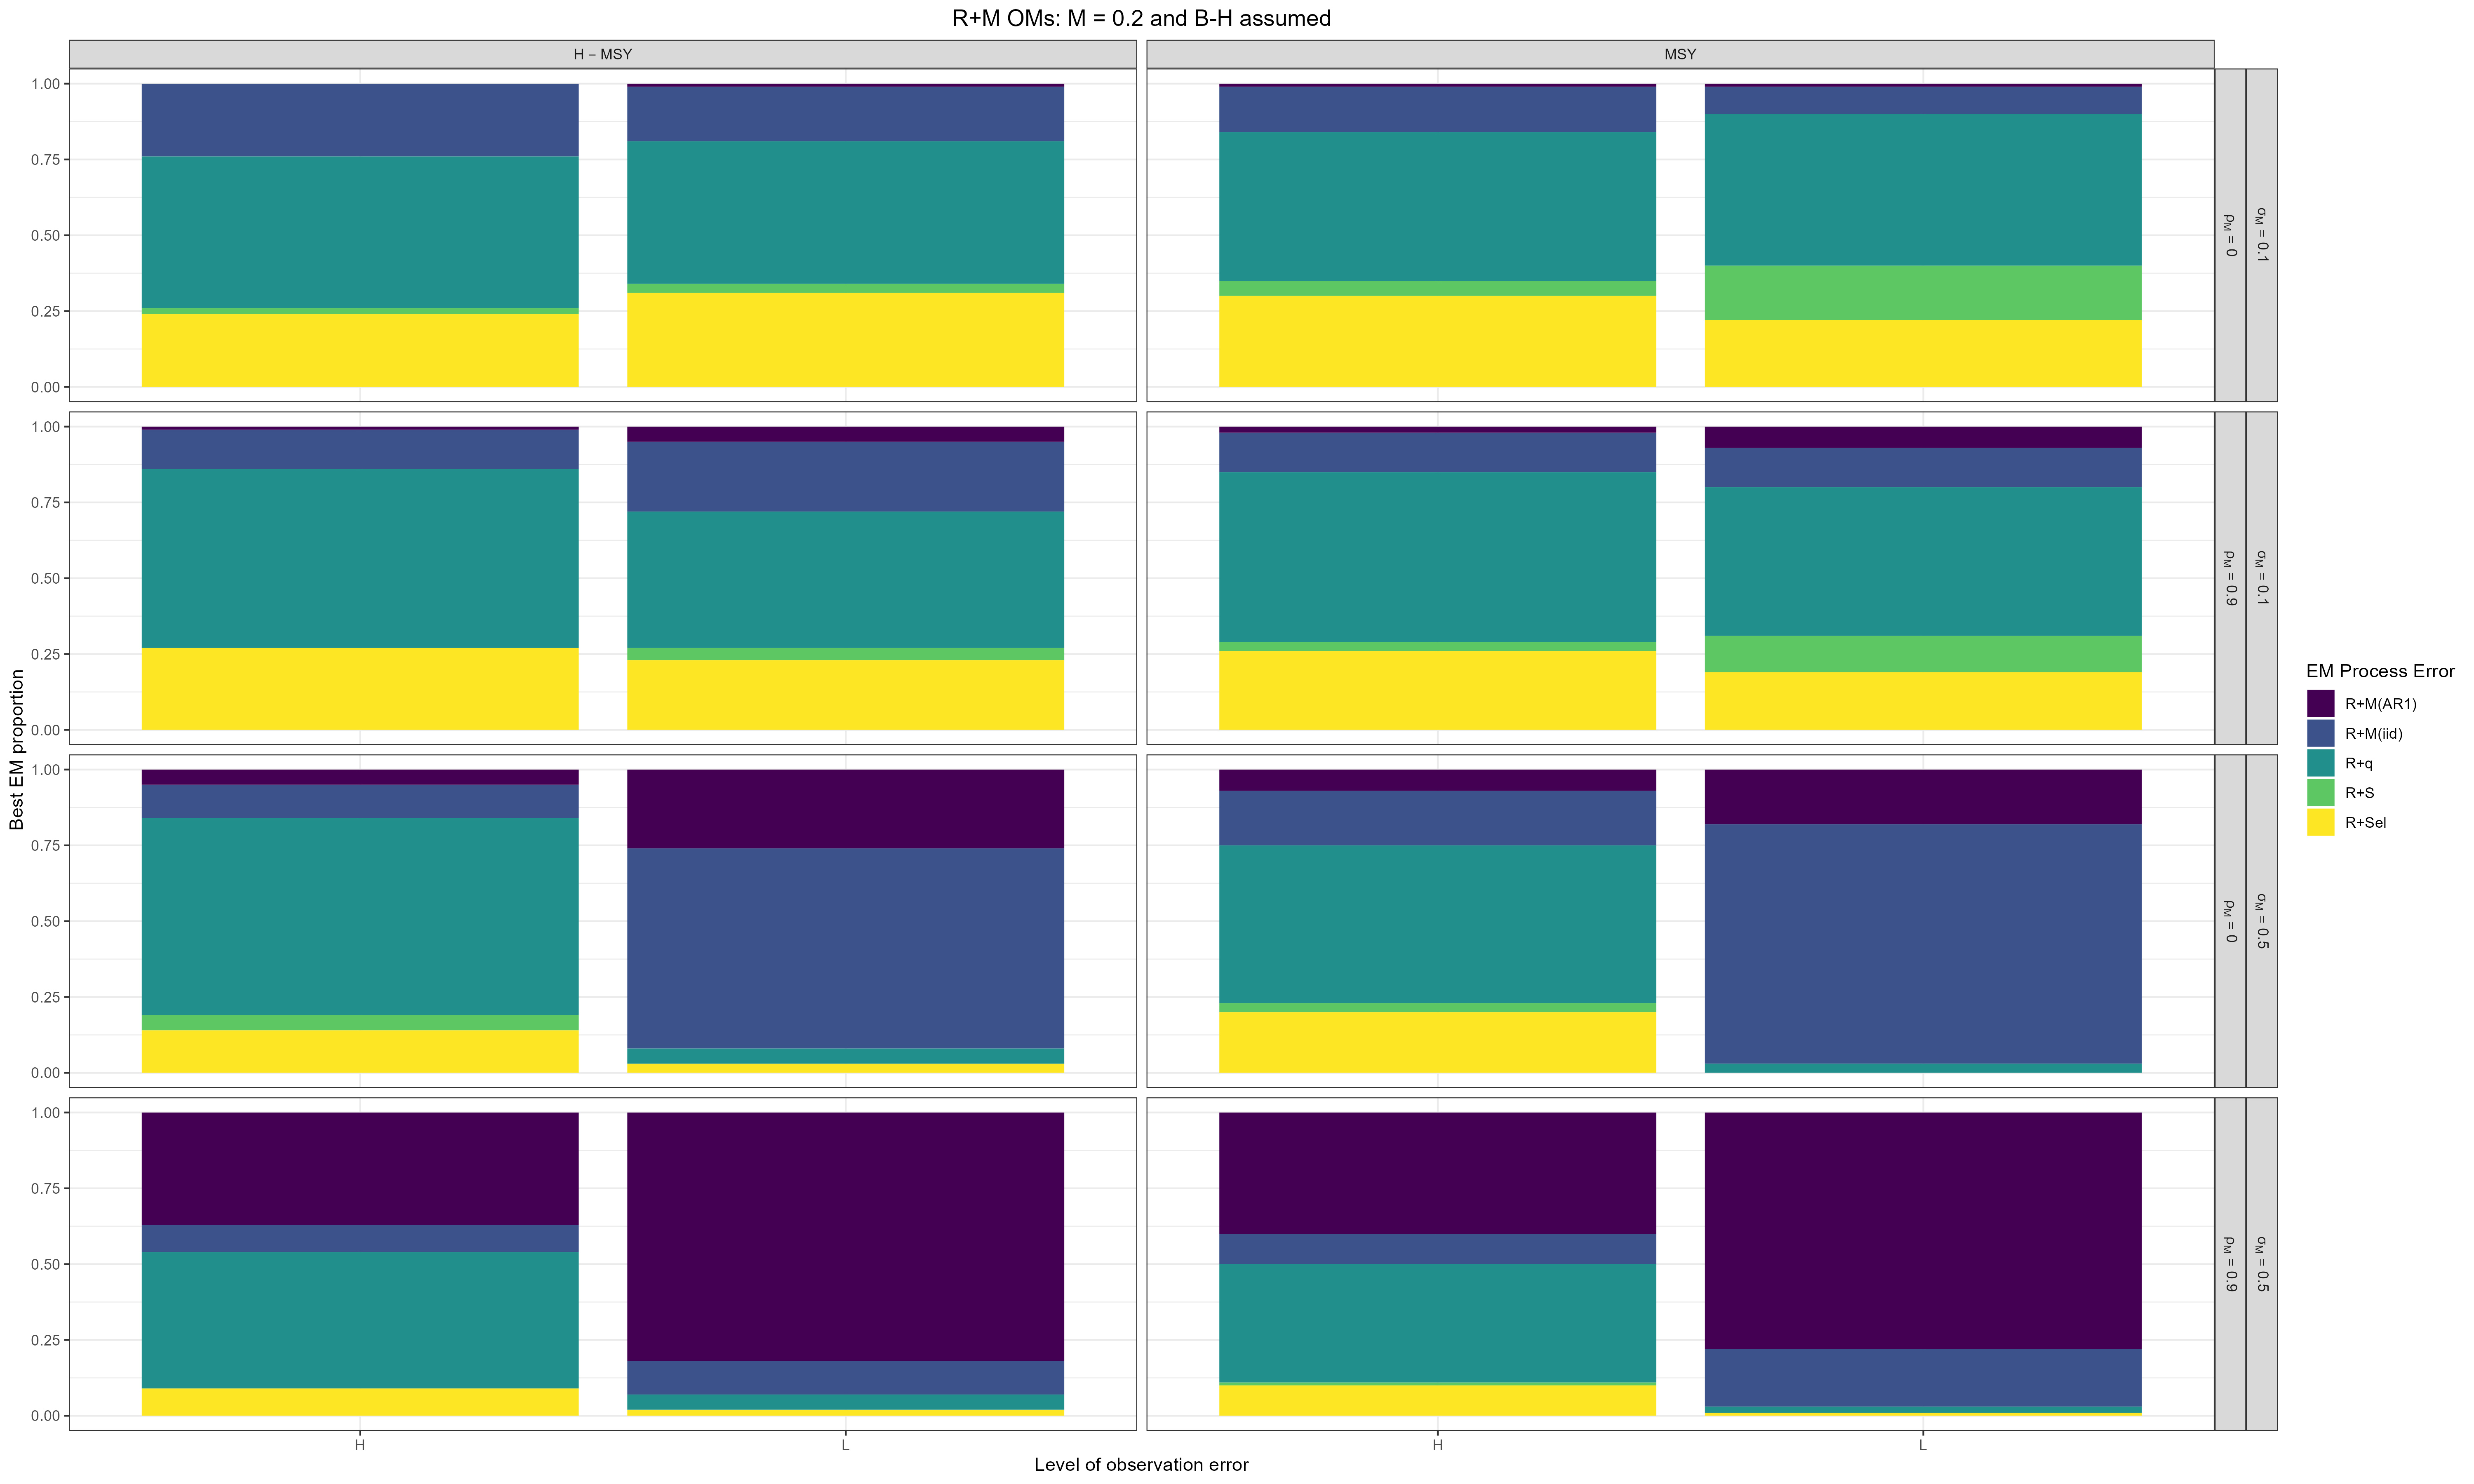
\includegraphics[width = \textwidth]{M_om_proportion_best_aic_SR_MF.png}
\end{center}
\end{figure}
\end{landscape}

\begin{landscape}
\begin{figure}
\caption{Proportion of simulated data sets from OMs with R+M process errors where fitted estimating models had lowest marginal AIC. All estimating models estimate a stock-recruit relationship and and M is estimated.} \label{M_om_proportion_best_aic_SR_ME}
\begin{center}
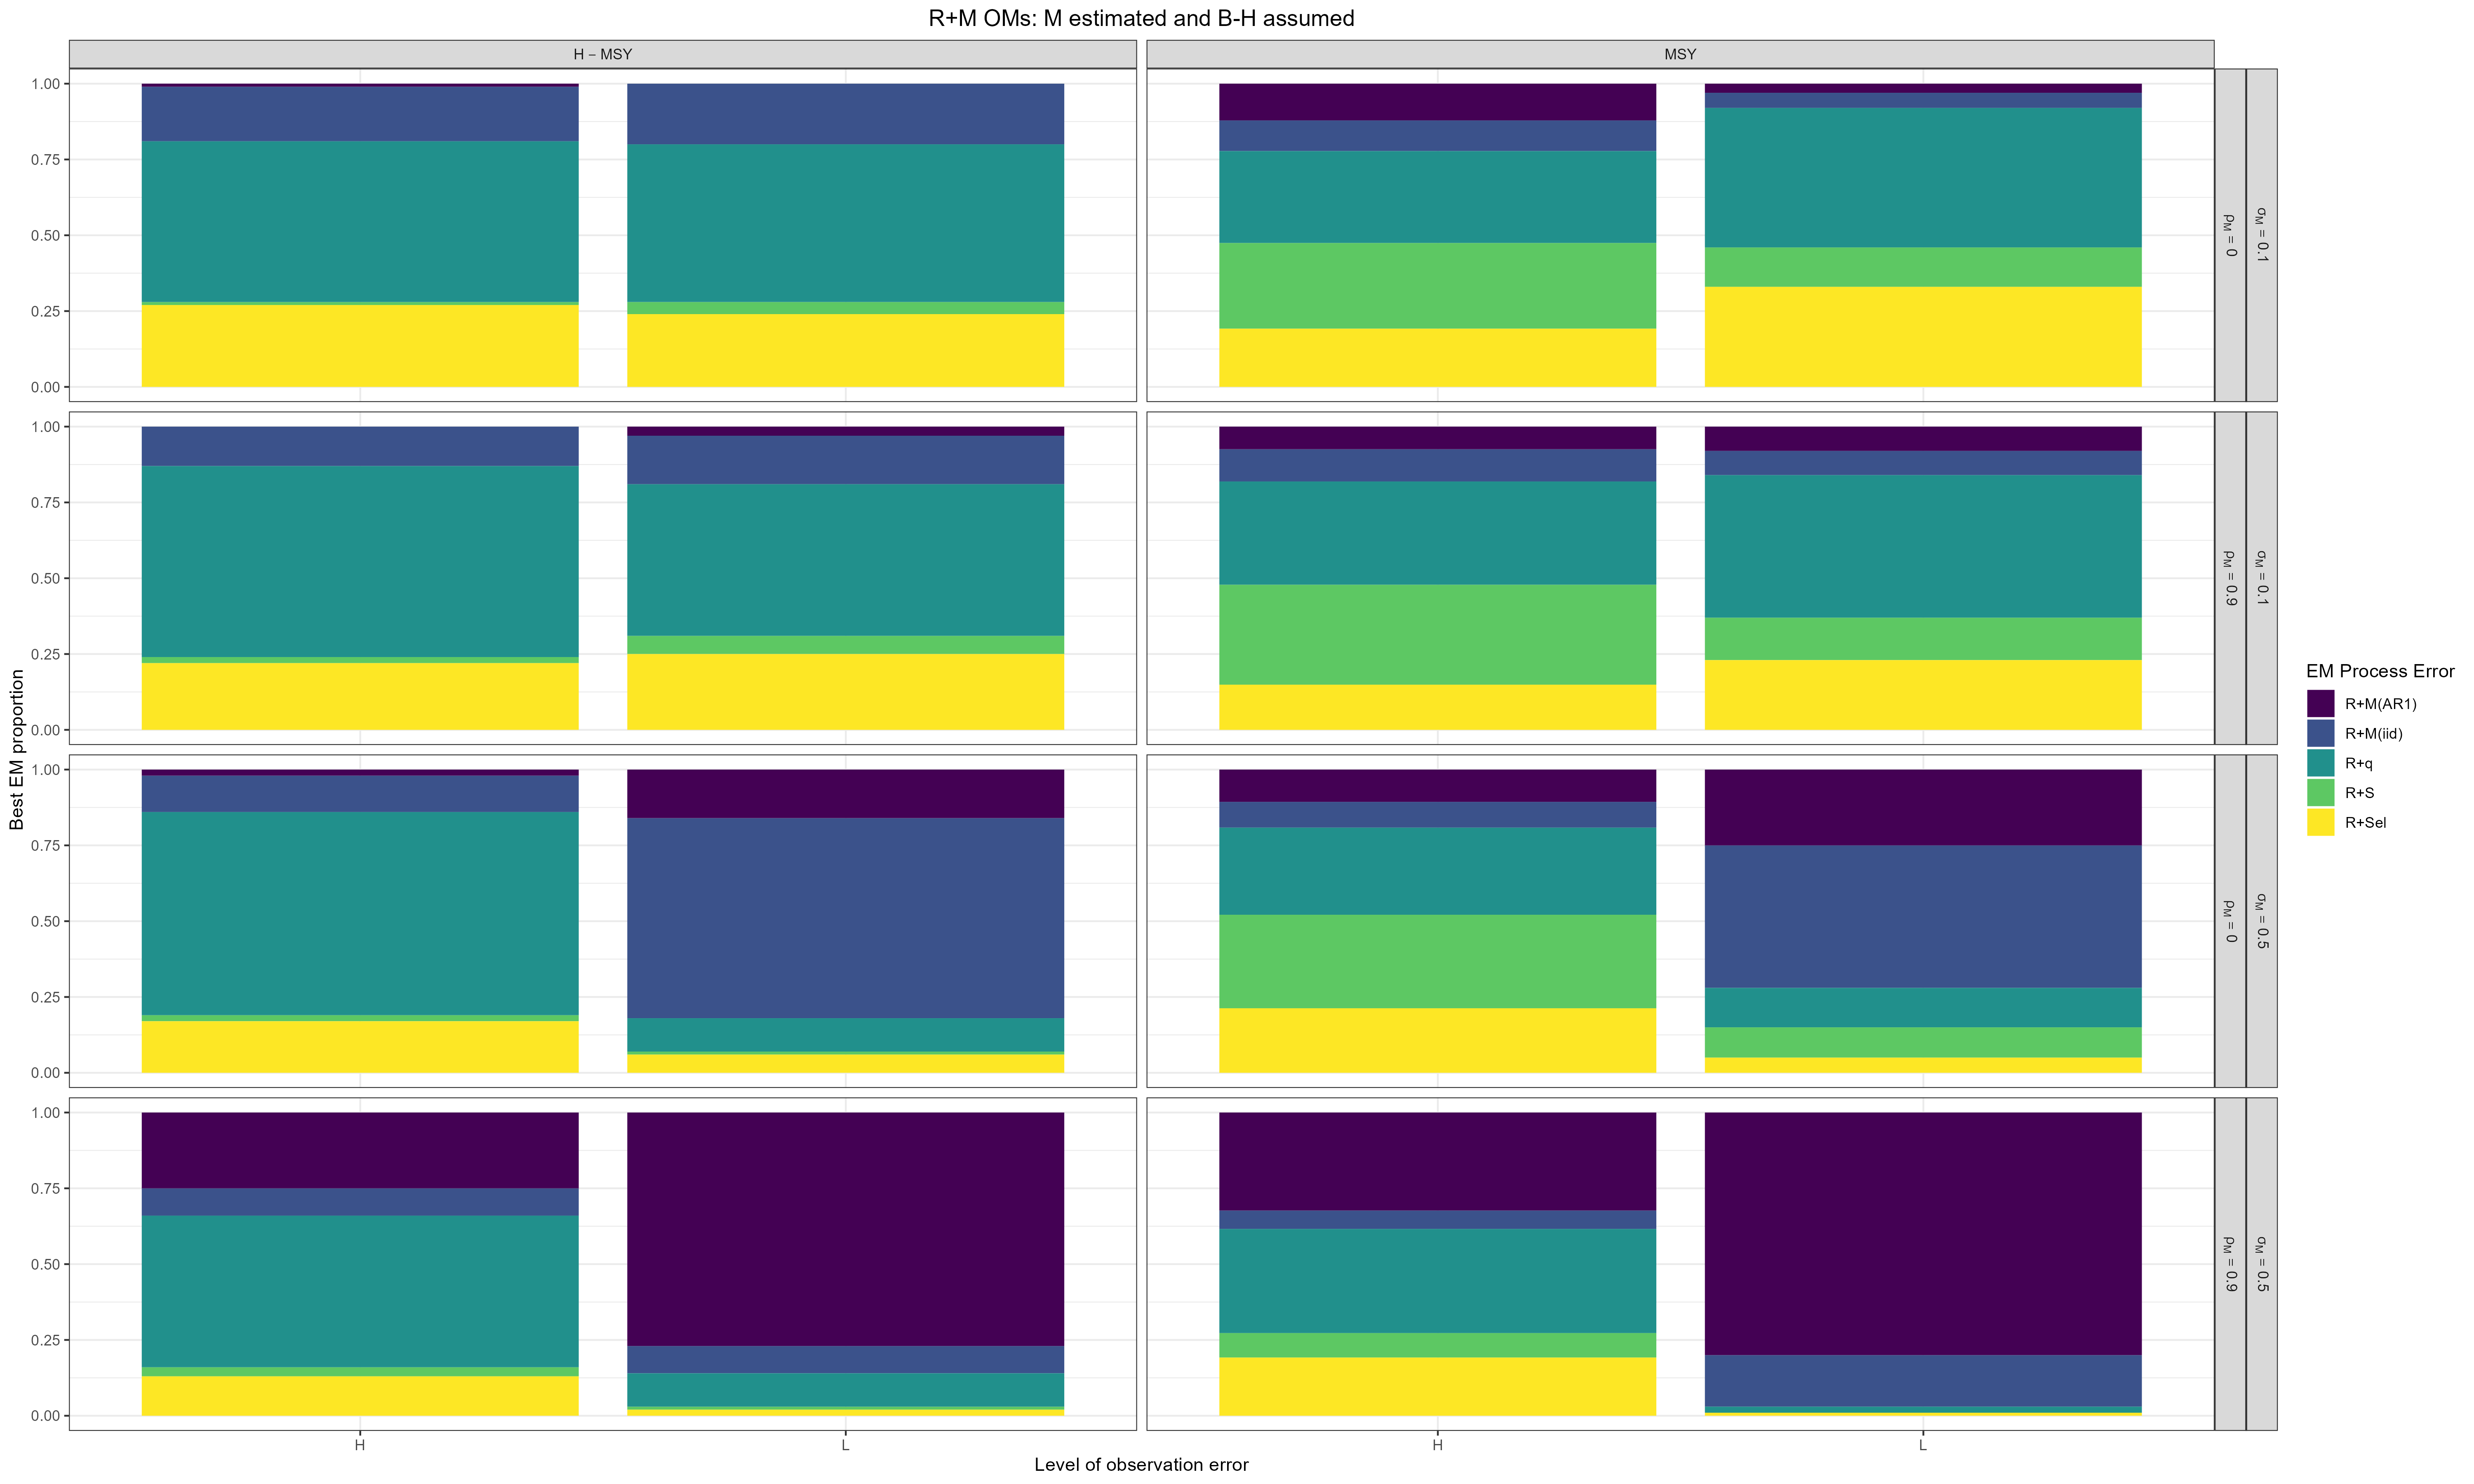
\includegraphics[width = \textwidth]{M_om_proportion_best_aic_SR_ME.png}
\end{center}
\end{figure}
\end{landscape}

\begin{landscape}
\begin{figure}
\caption{Proportion of simulated data sets from OMs with R+Sel process errors where fitted estimating models had lowest marginal AIC. All estimating models estimate mean recruitment rather than a stock-recruit relationship and and M is fixed at the true value.} \label{Sel_om_proportion_best_aic_R_MF}
\begin{center}
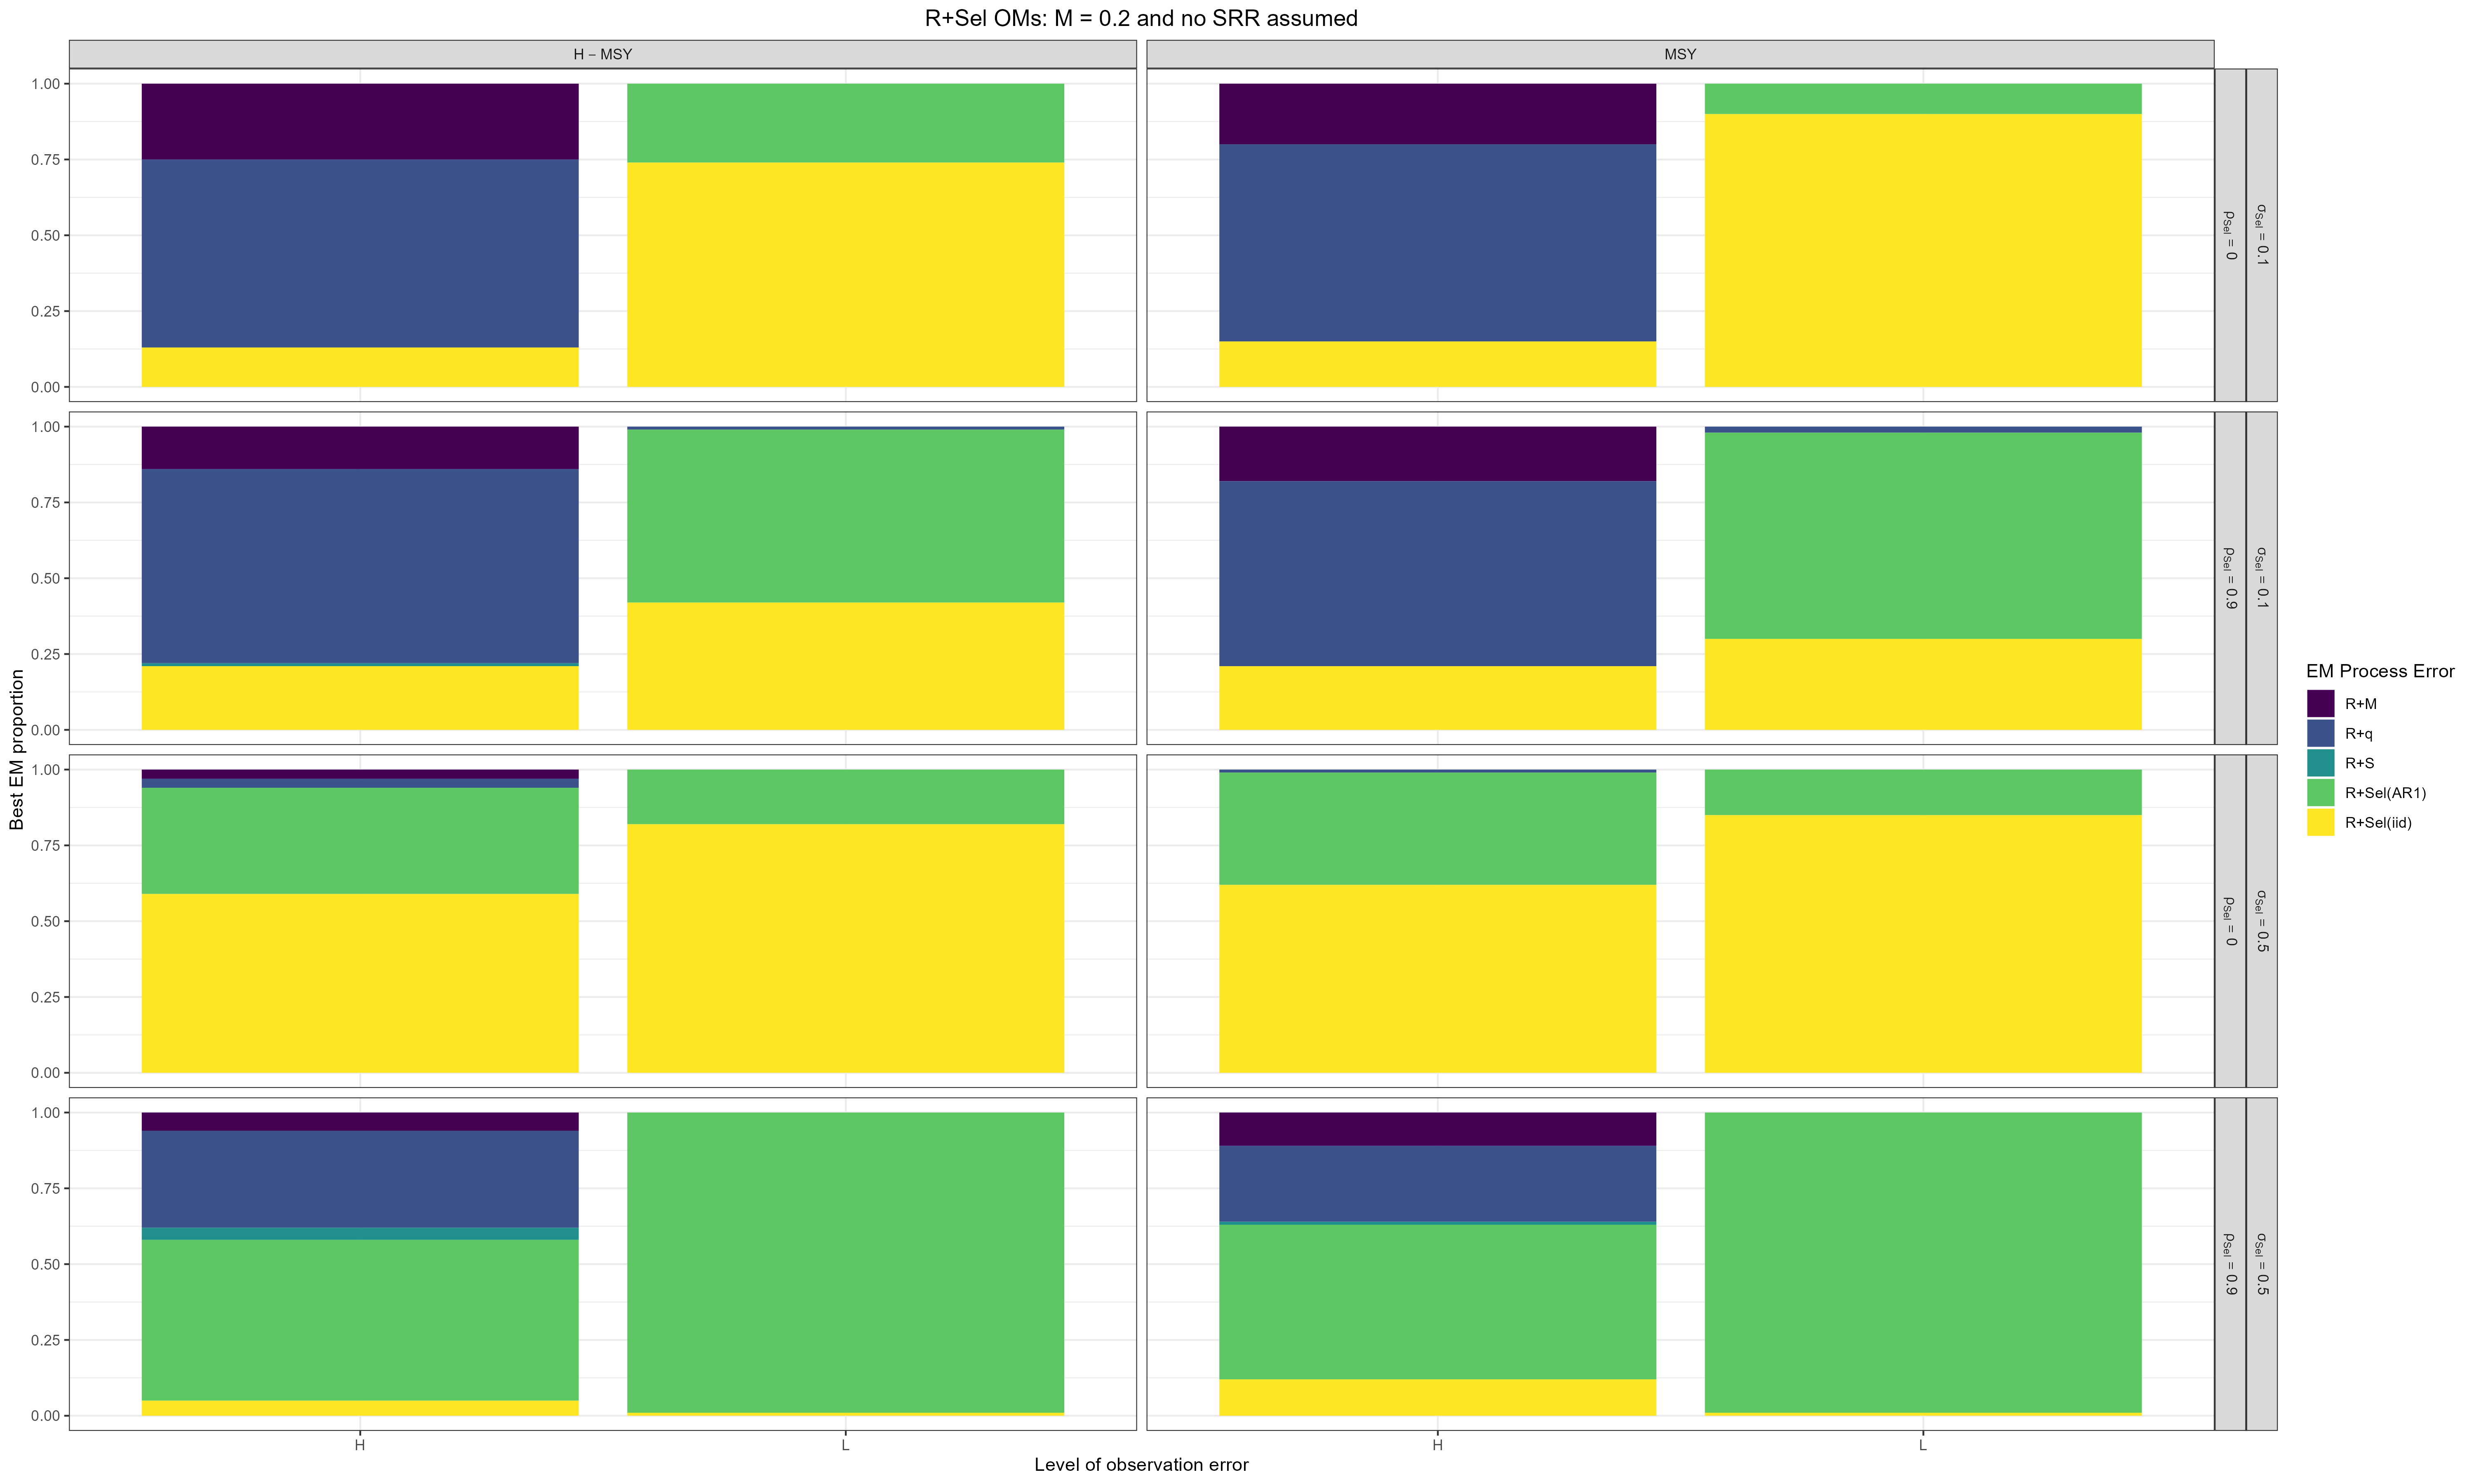
\includegraphics[width = \textwidth]{Sel_om_proportion_best_aic_R_MF.png}
\end{center}
\end{figure}
\end{landscape}

\begin{landscape}
\begin{figure}
\caption{Proportion of simulated data sets from OMs with R+Sel process errors where fitted estimating models had lowest marginal AIC. All estimating models estimate mean recruitment rather than a stock-recruit relationship and and M is estimated.} \label{Sel_om_proportion_best_aic_R_ME}
\begin{center}
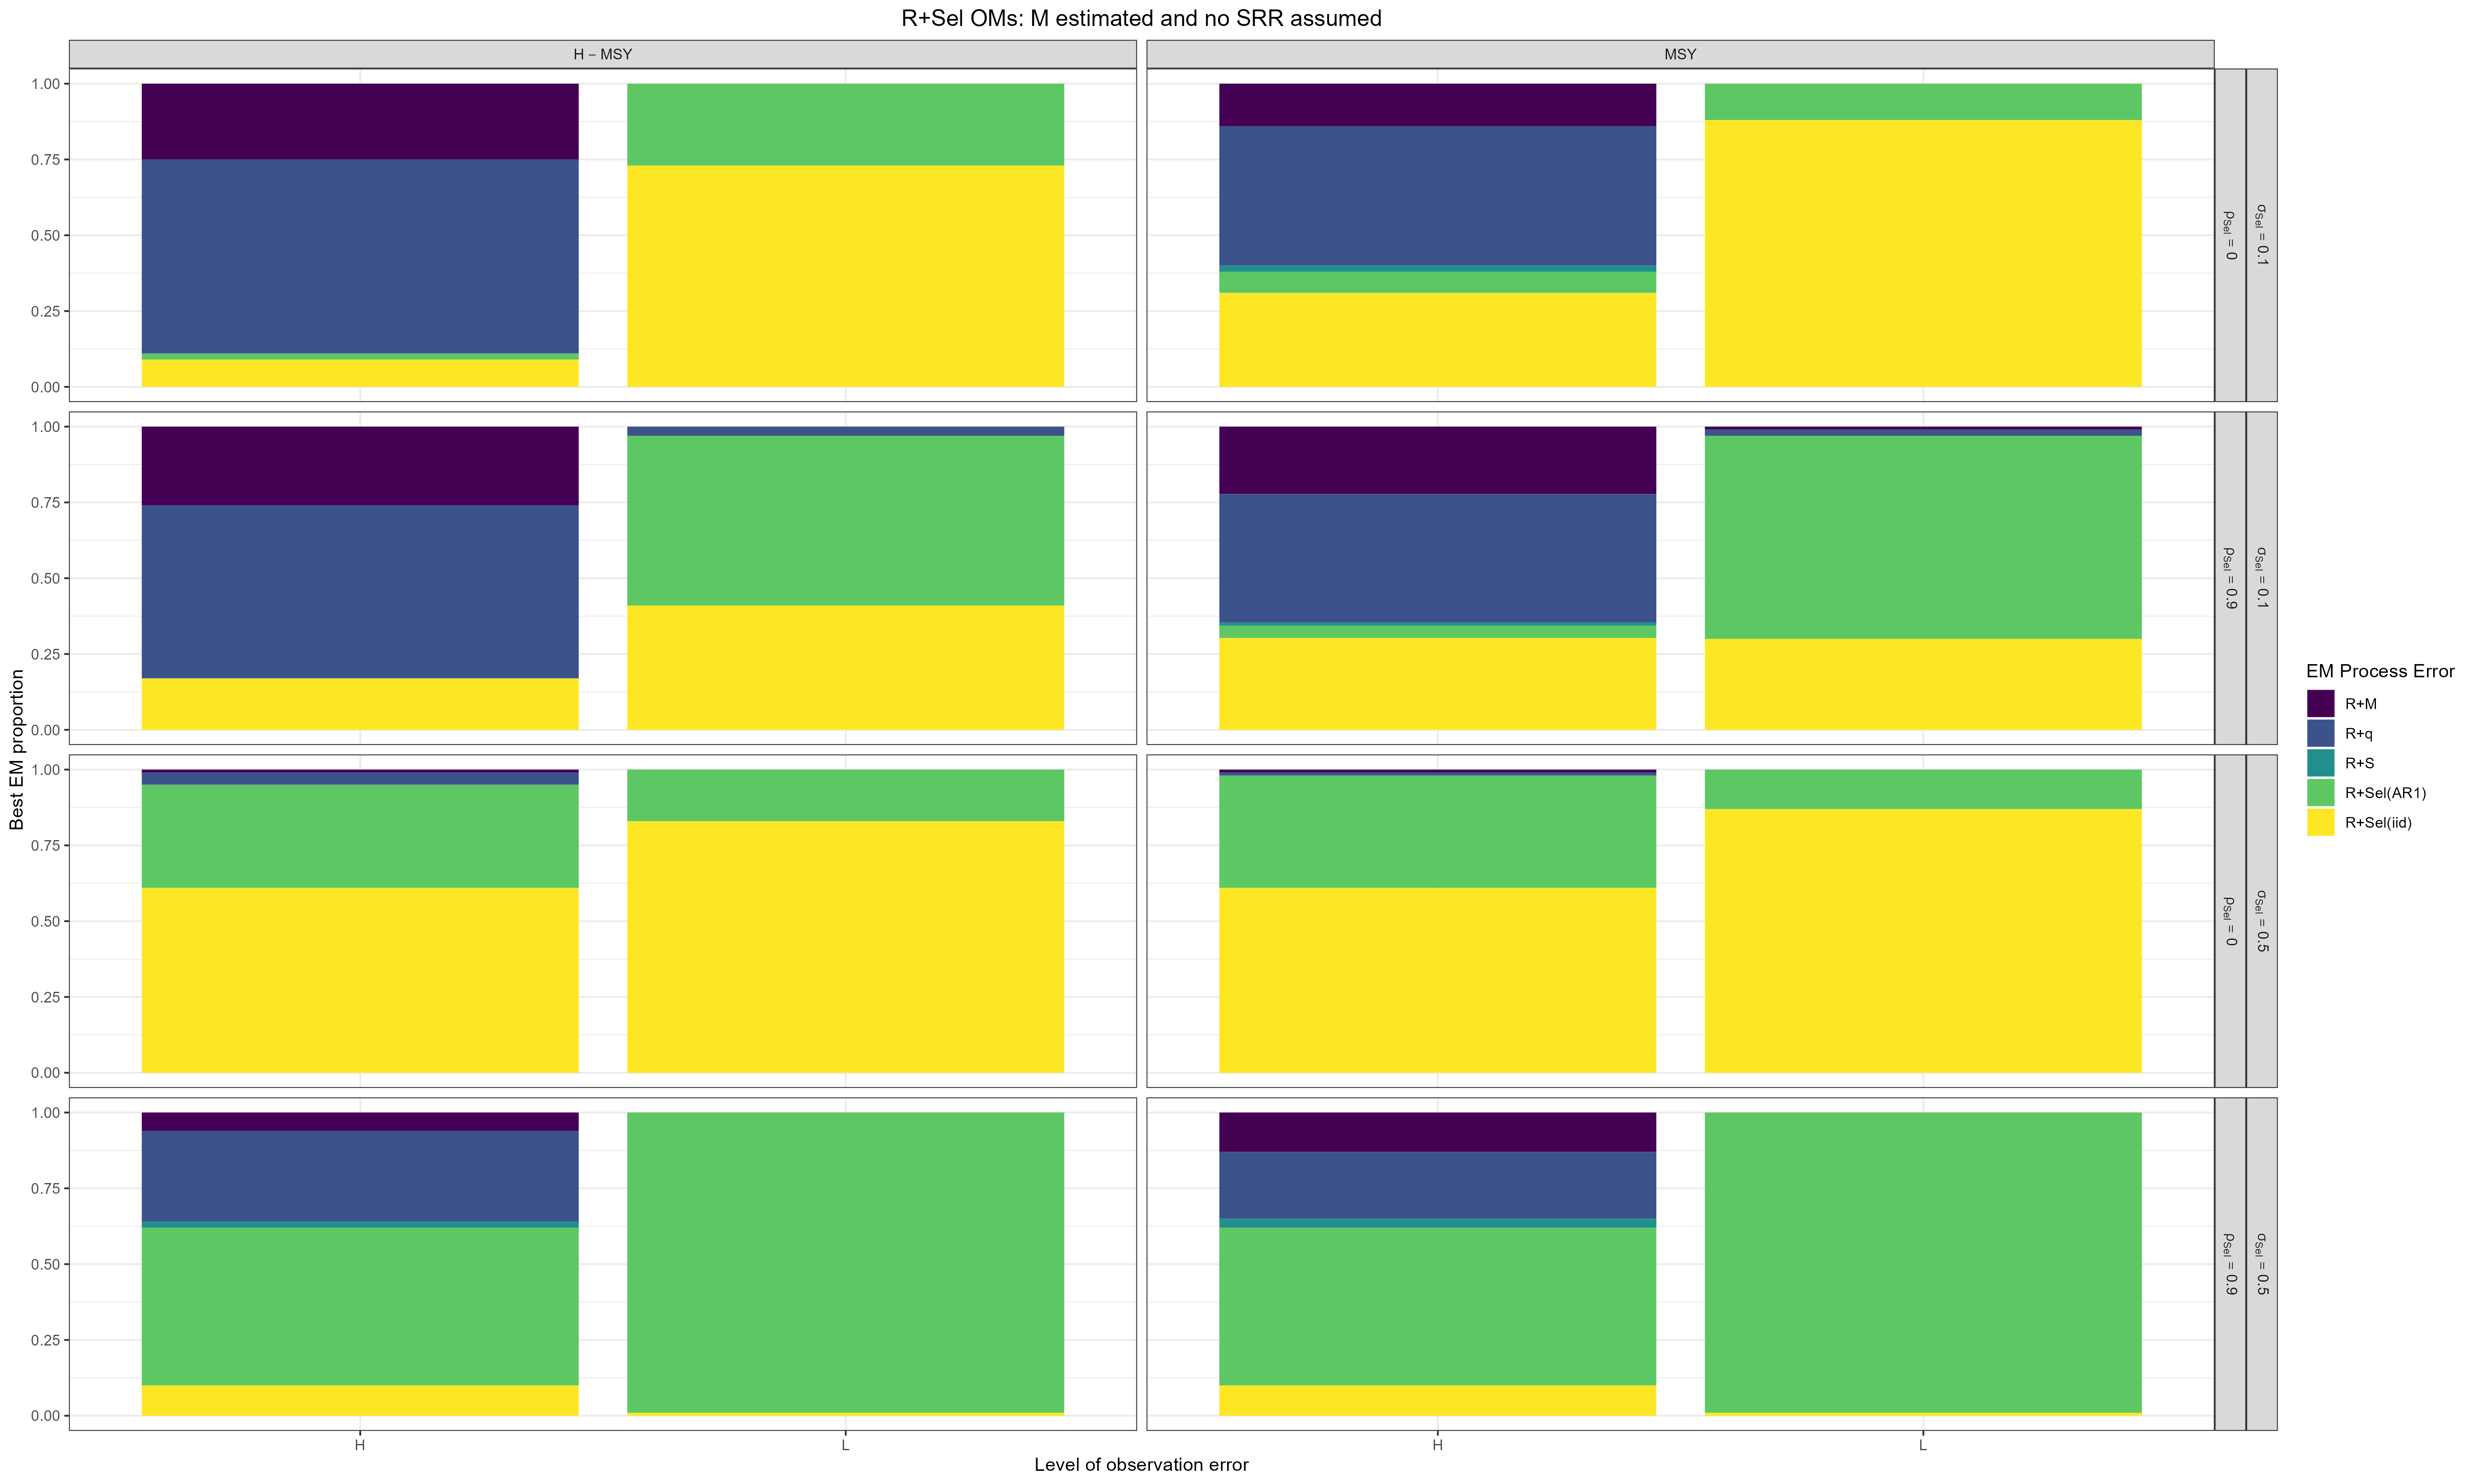
\includegraphics[width = \textwidth]{Sel_om_proportion_best_aic_R_ME.png}
\end{center}
\end{figure}
\end{landscape}

\begin{landscape}
\begin{figure}
\caption{Proportion of simulated data sets from OMs with R+Sel process errors where fitted estimating models had lowest marginal AIC. All estimating models estimate a stock-recruit relationship and and M is fixed at the true value.} \label{Sel_om_proportion_best_aic_SR_MF}
\begin{center}
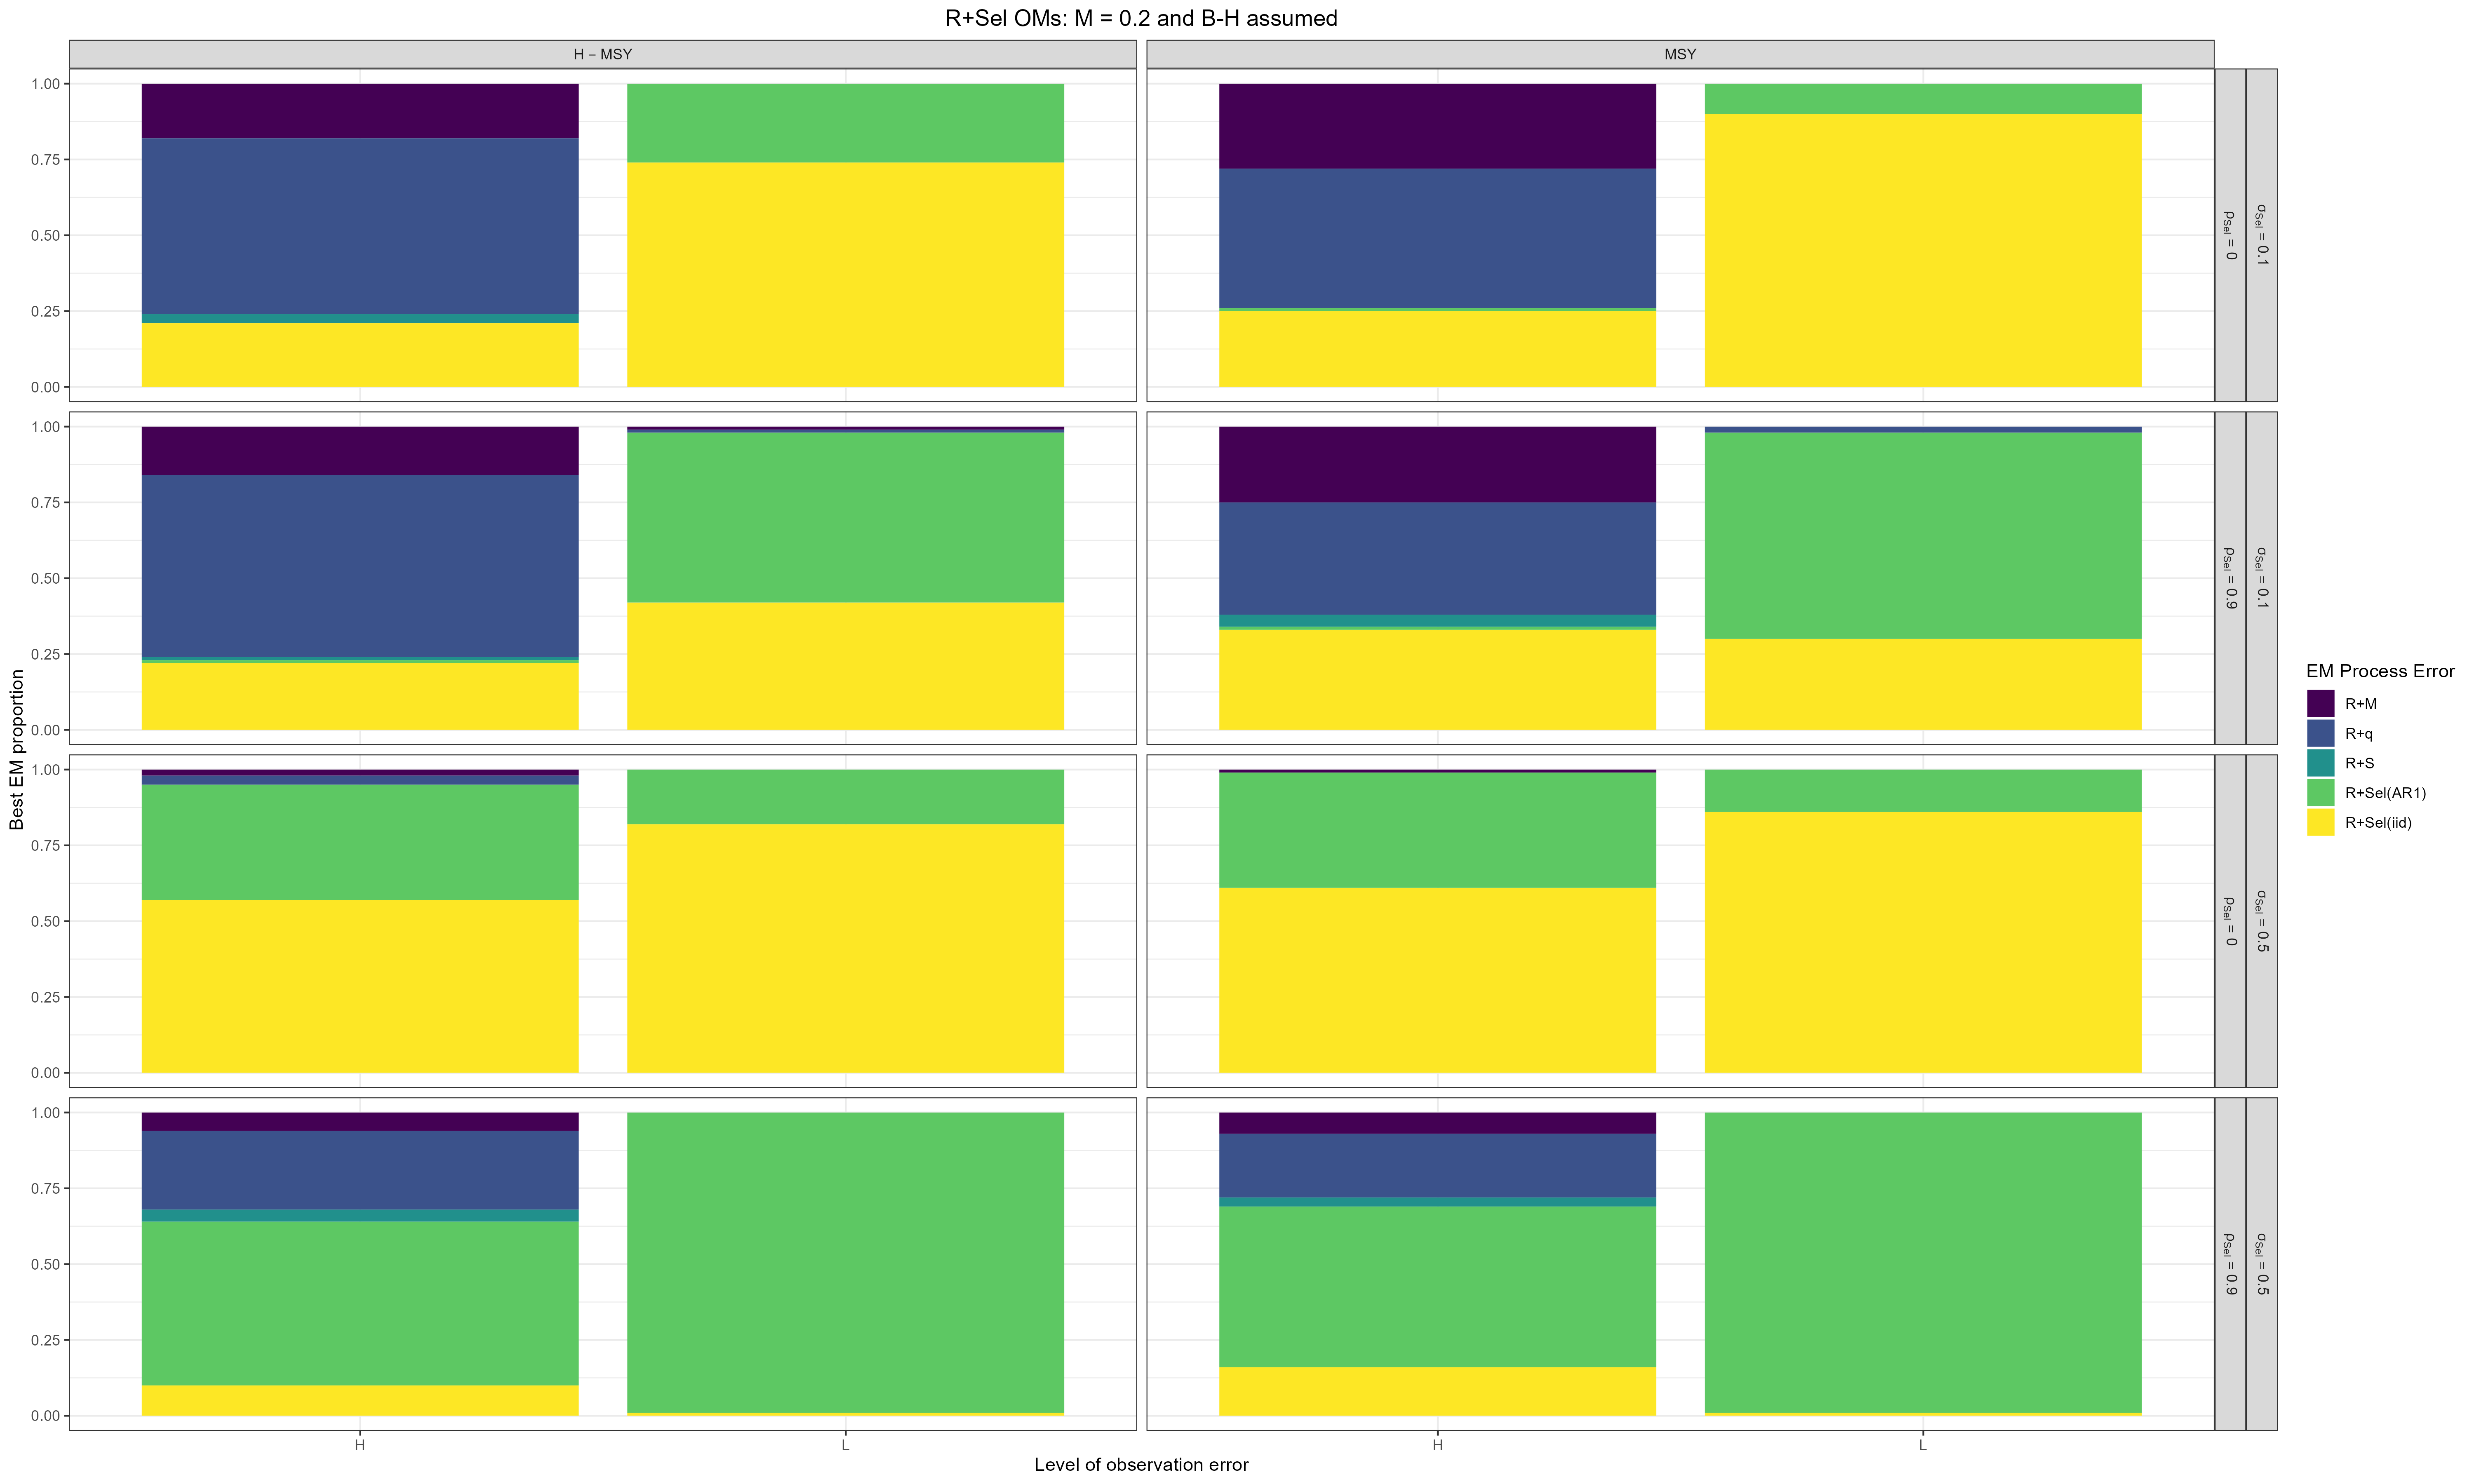
\includegraphics[width = \textwidth]{Sel_om_proportion_best_aic_SR_MF.png}
\end{center}
\end{figure}
\end{landscape}

\begin{landscape}
\begin{figure}
\caption{Proportion of simulated data sets from OMs with R+Sel process errors where fitted estimating models had lowest marginal AIC. All estimating models estimate a stock-recruit relationship and and M is estimated.} \label{Sel_om_proportion_best_aic_SR_ME}
\begin{center}
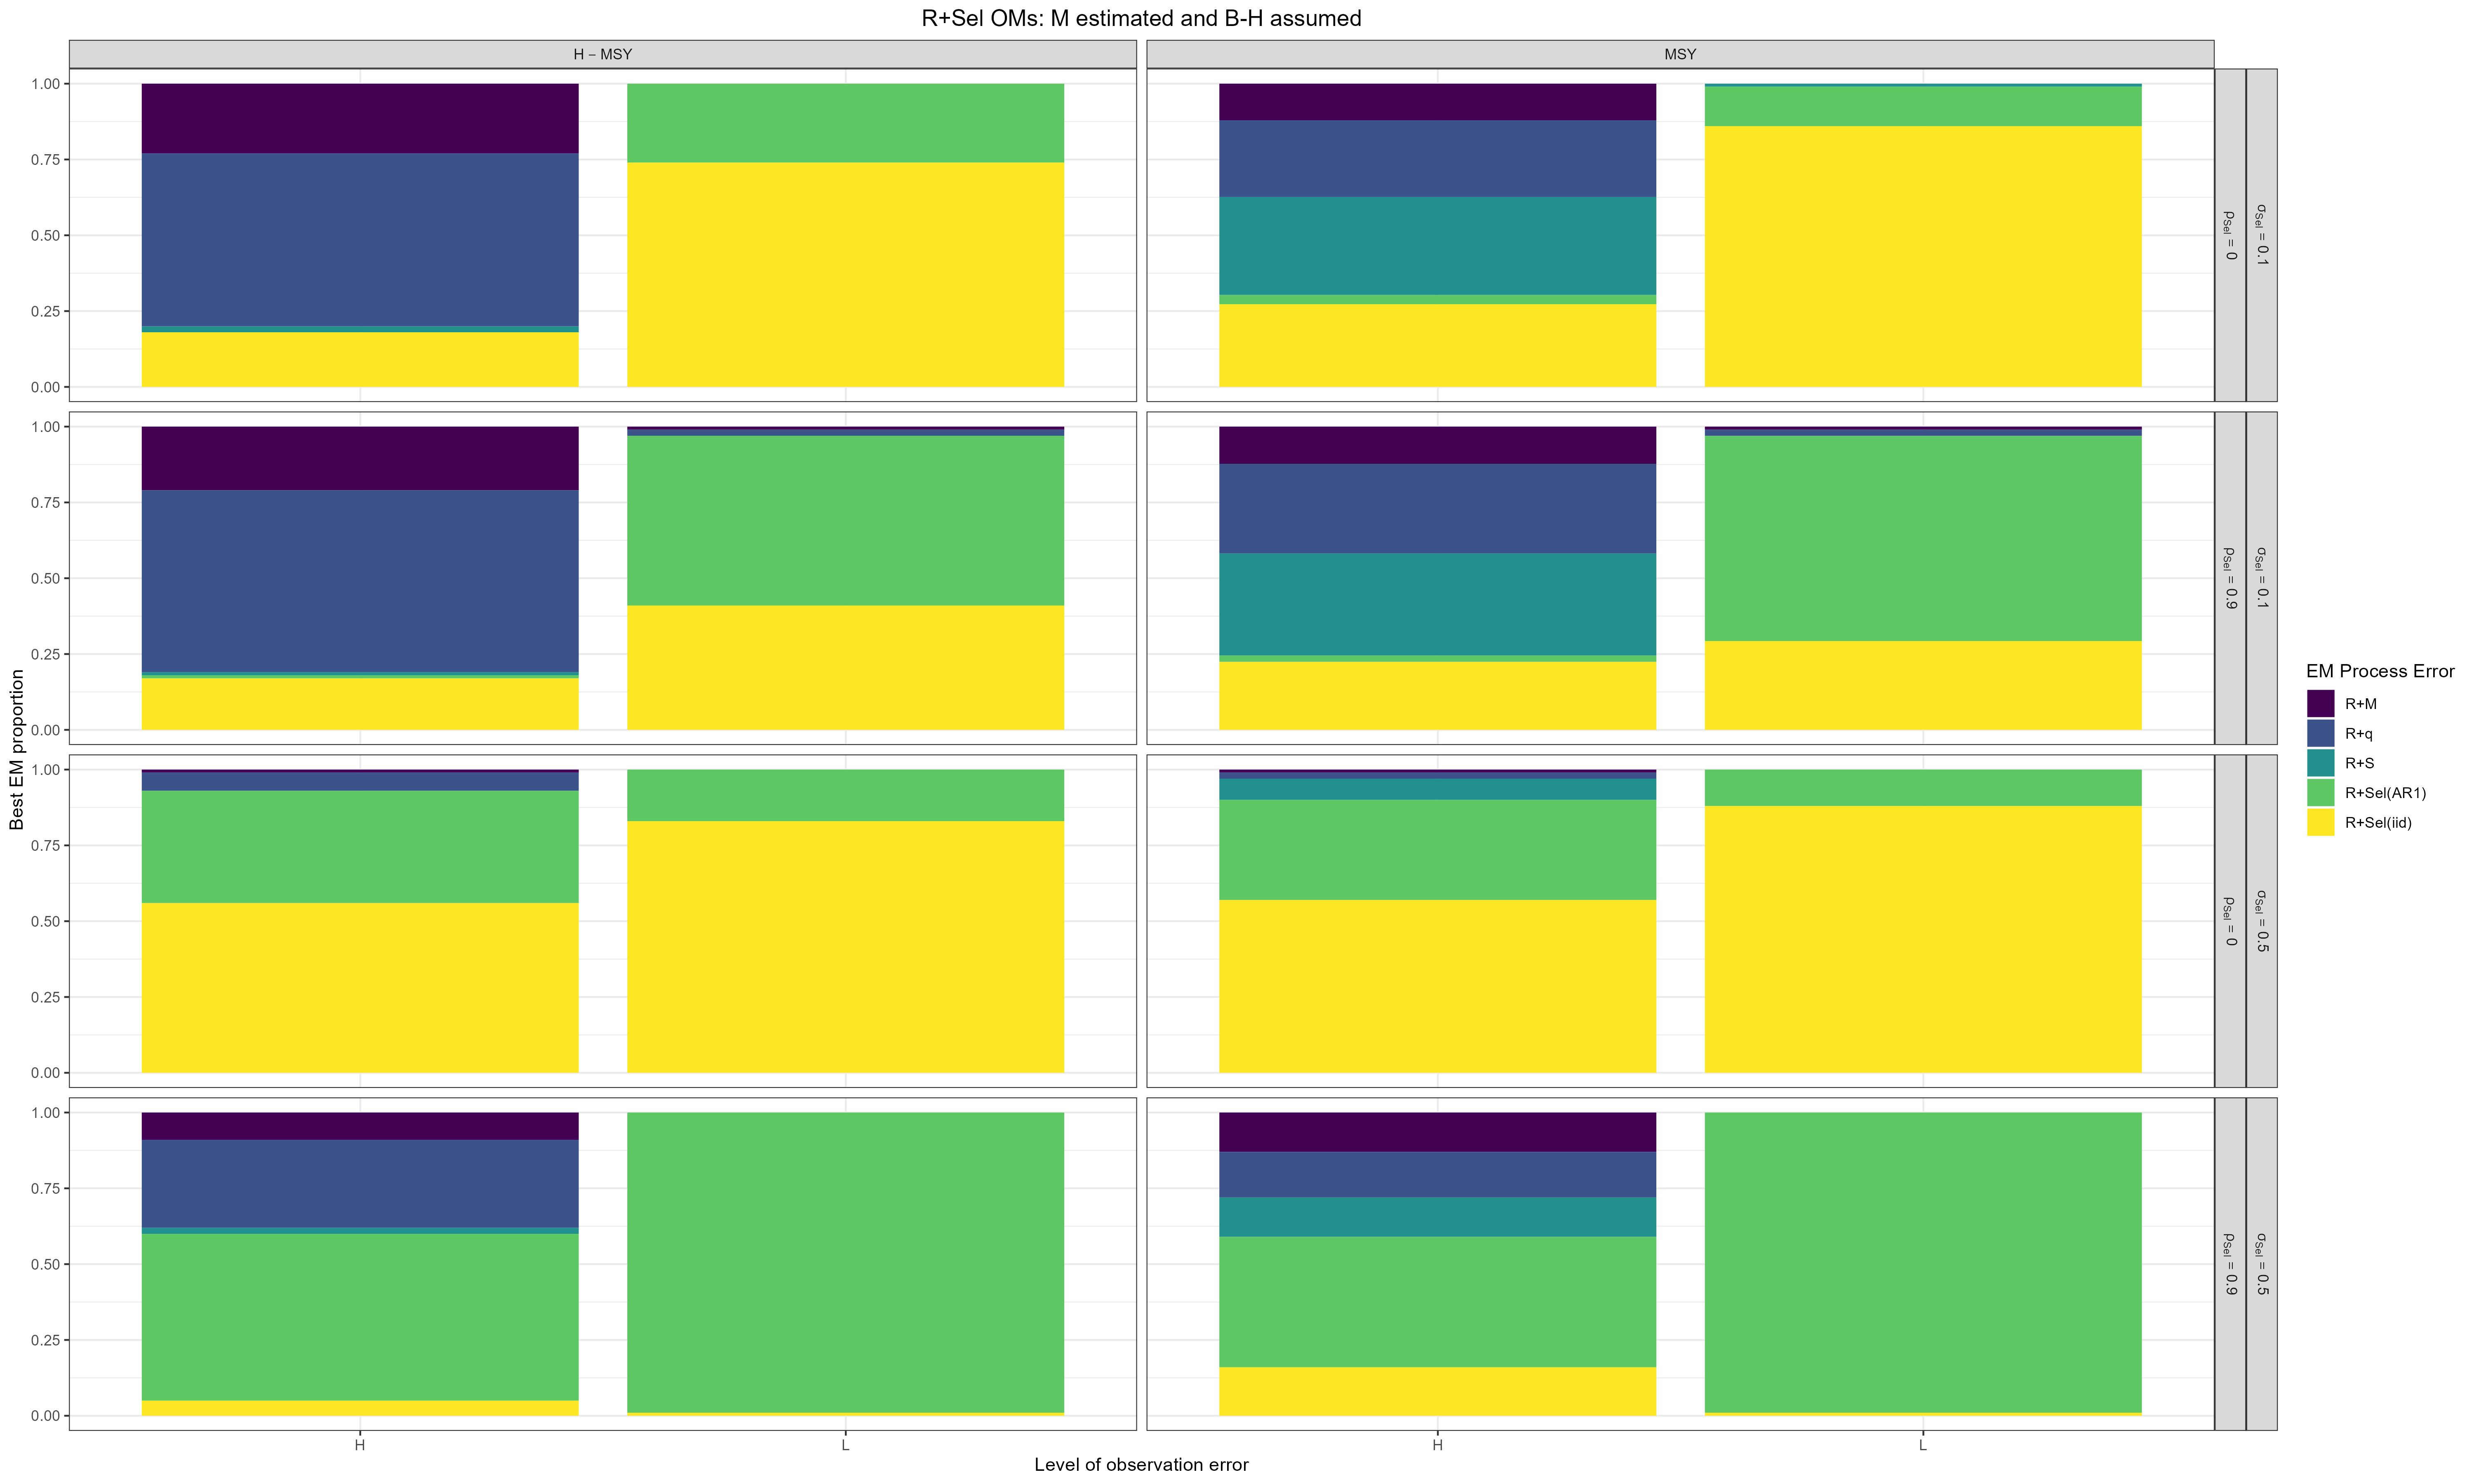
\includegraphics[width = \textwidth]{Sel_om_proportion_best_aic_SR_ME.png}
\end{center}
\end{figure}
\end{landscape}

\begin{landscape}
\begin{figure}
\caption{Proportion of simulated data sets from OMs with R+q process errors where fitted estimating models had lowest marginal AIC. All estimating models estimate mean recruitment rather than a stock-recruit relationship and and M is fixed at the true value.} \label{q_om_proportion_best_aic_R_MF}
\begin{center}
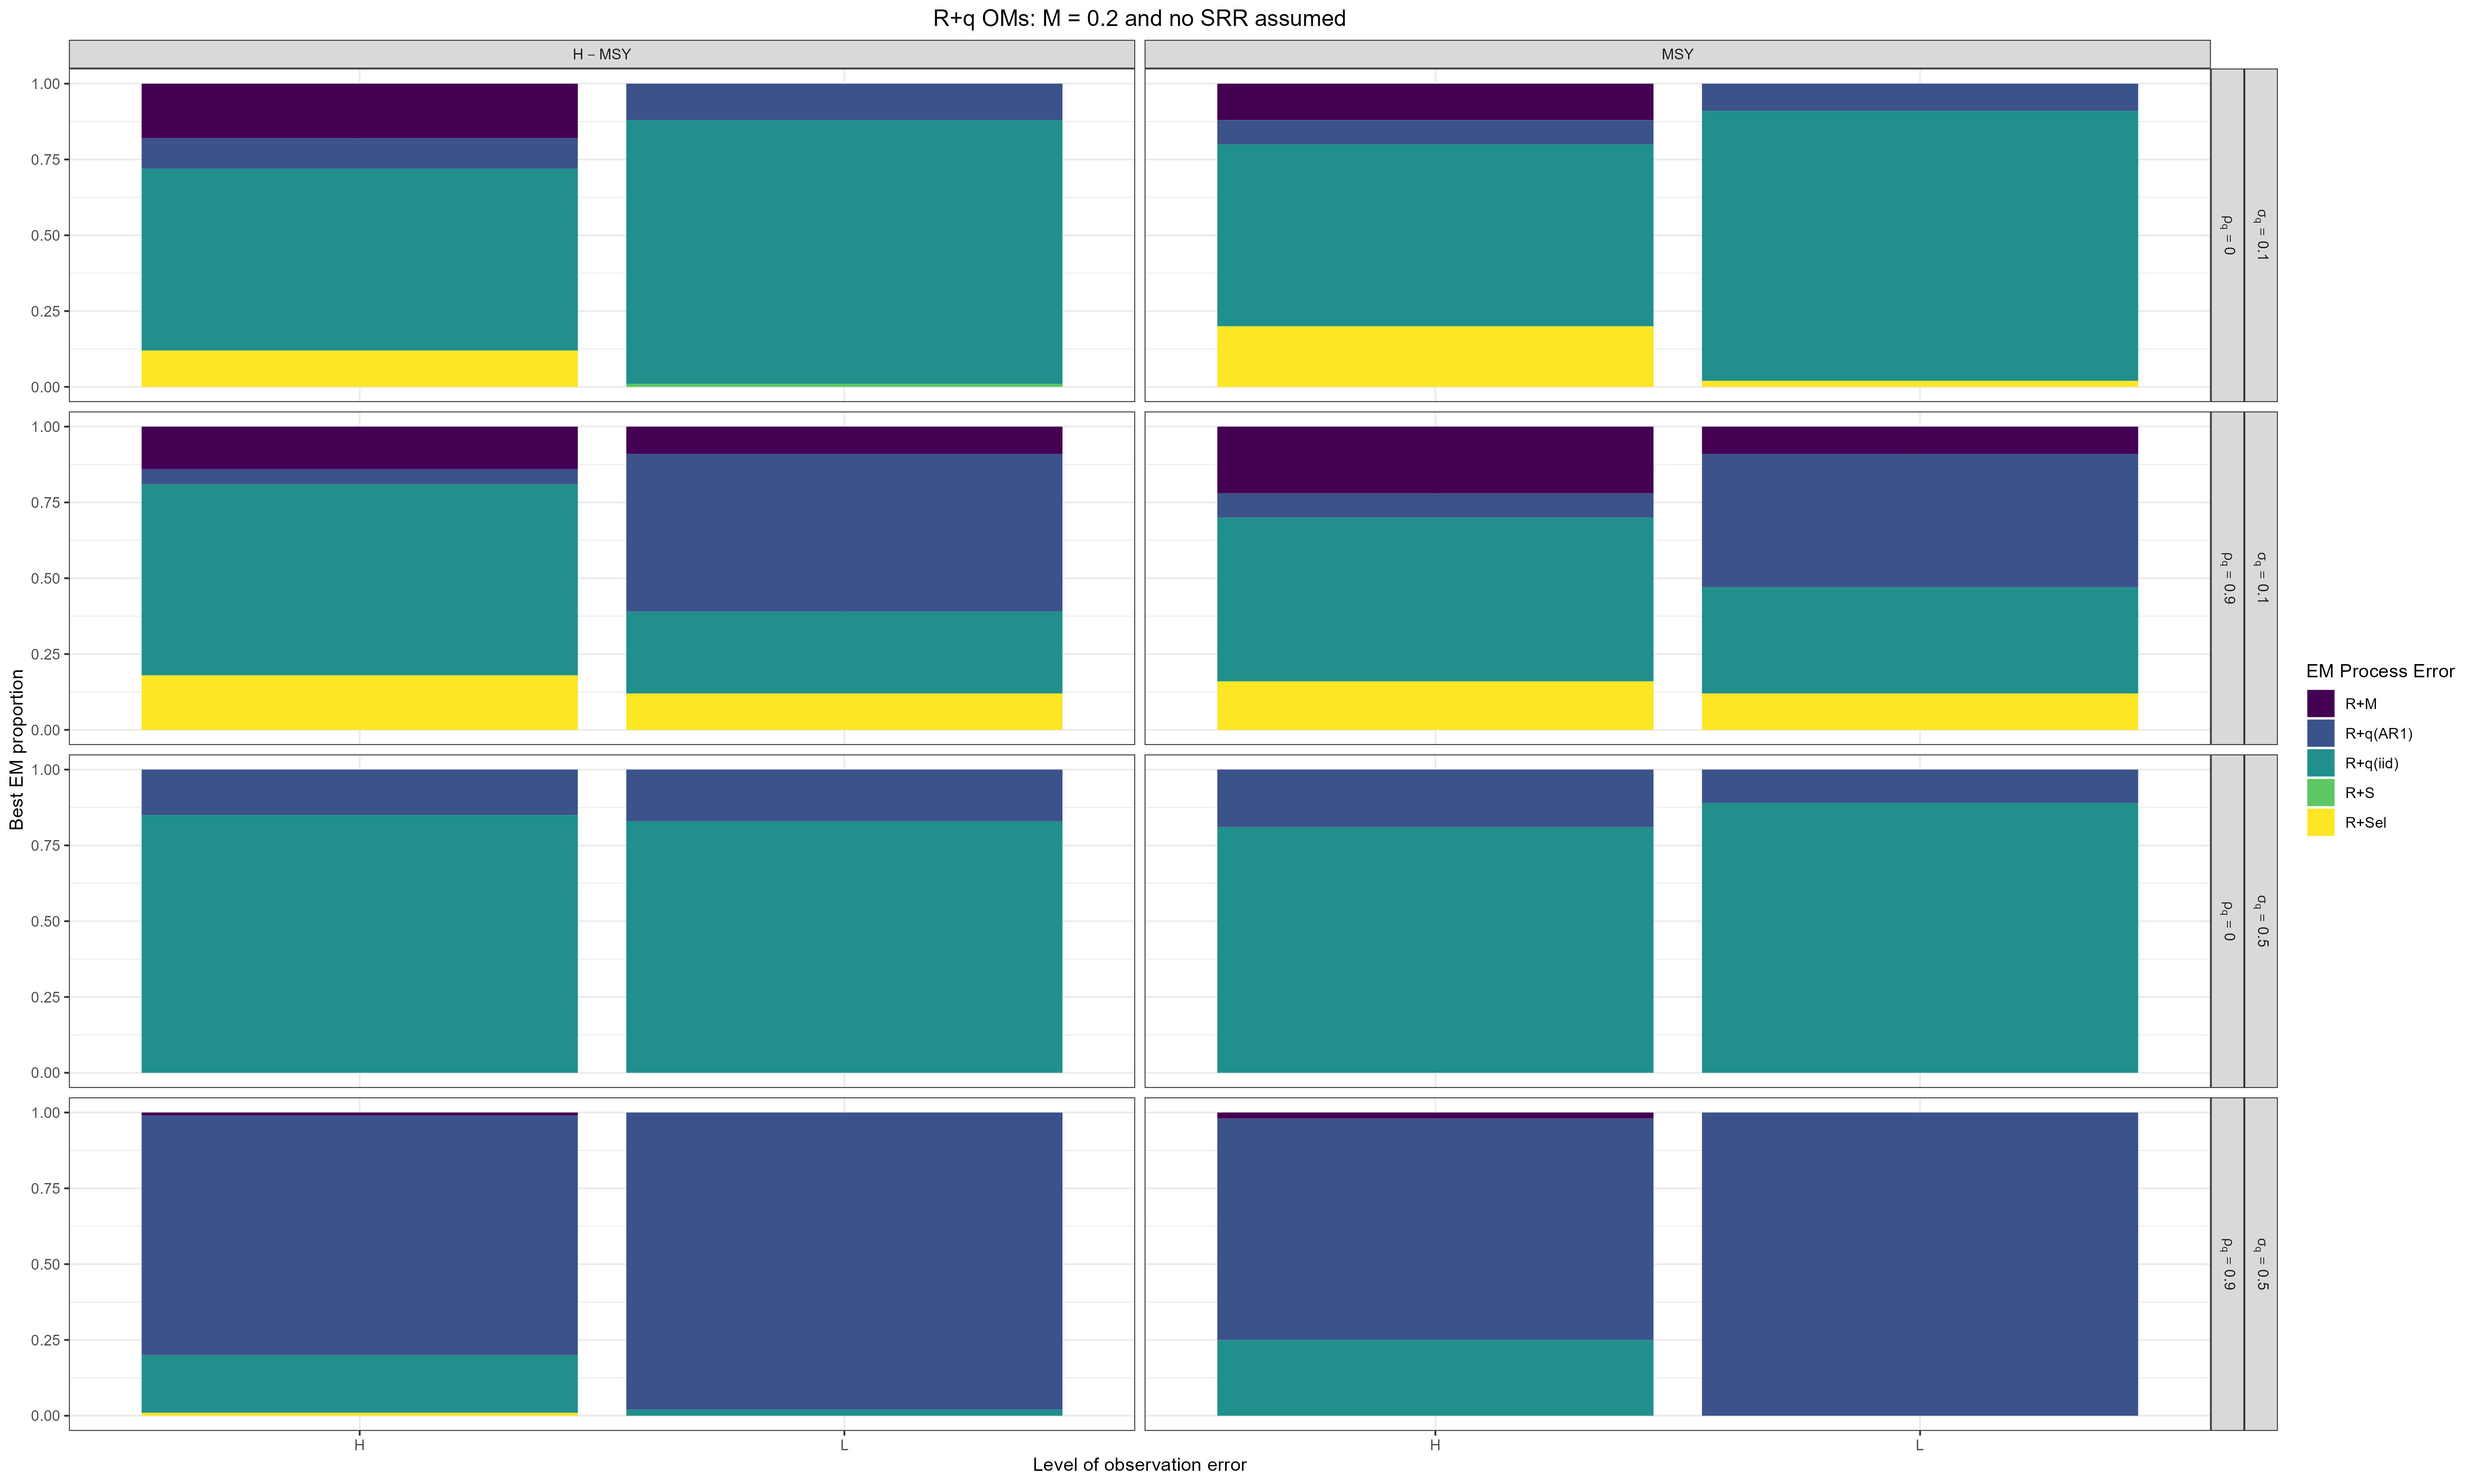
\includegraphics[width = \textwidth]{q_om_proportion_best_aic_R_MF.png}
\end{center}
\end{figure}
\end{landscape}

\begin{landscape}
\begin{figure}
\caption{Proportion of simulated data sets from OMs with R+q process errors where fitted estimating models had lowest marginal AIC. All estimating models estimate mean recruitment rather than a stock-recruit relationship and and M is estimated.} \label{q_om_proportion_best_aic_R_ME}
\begin{center}
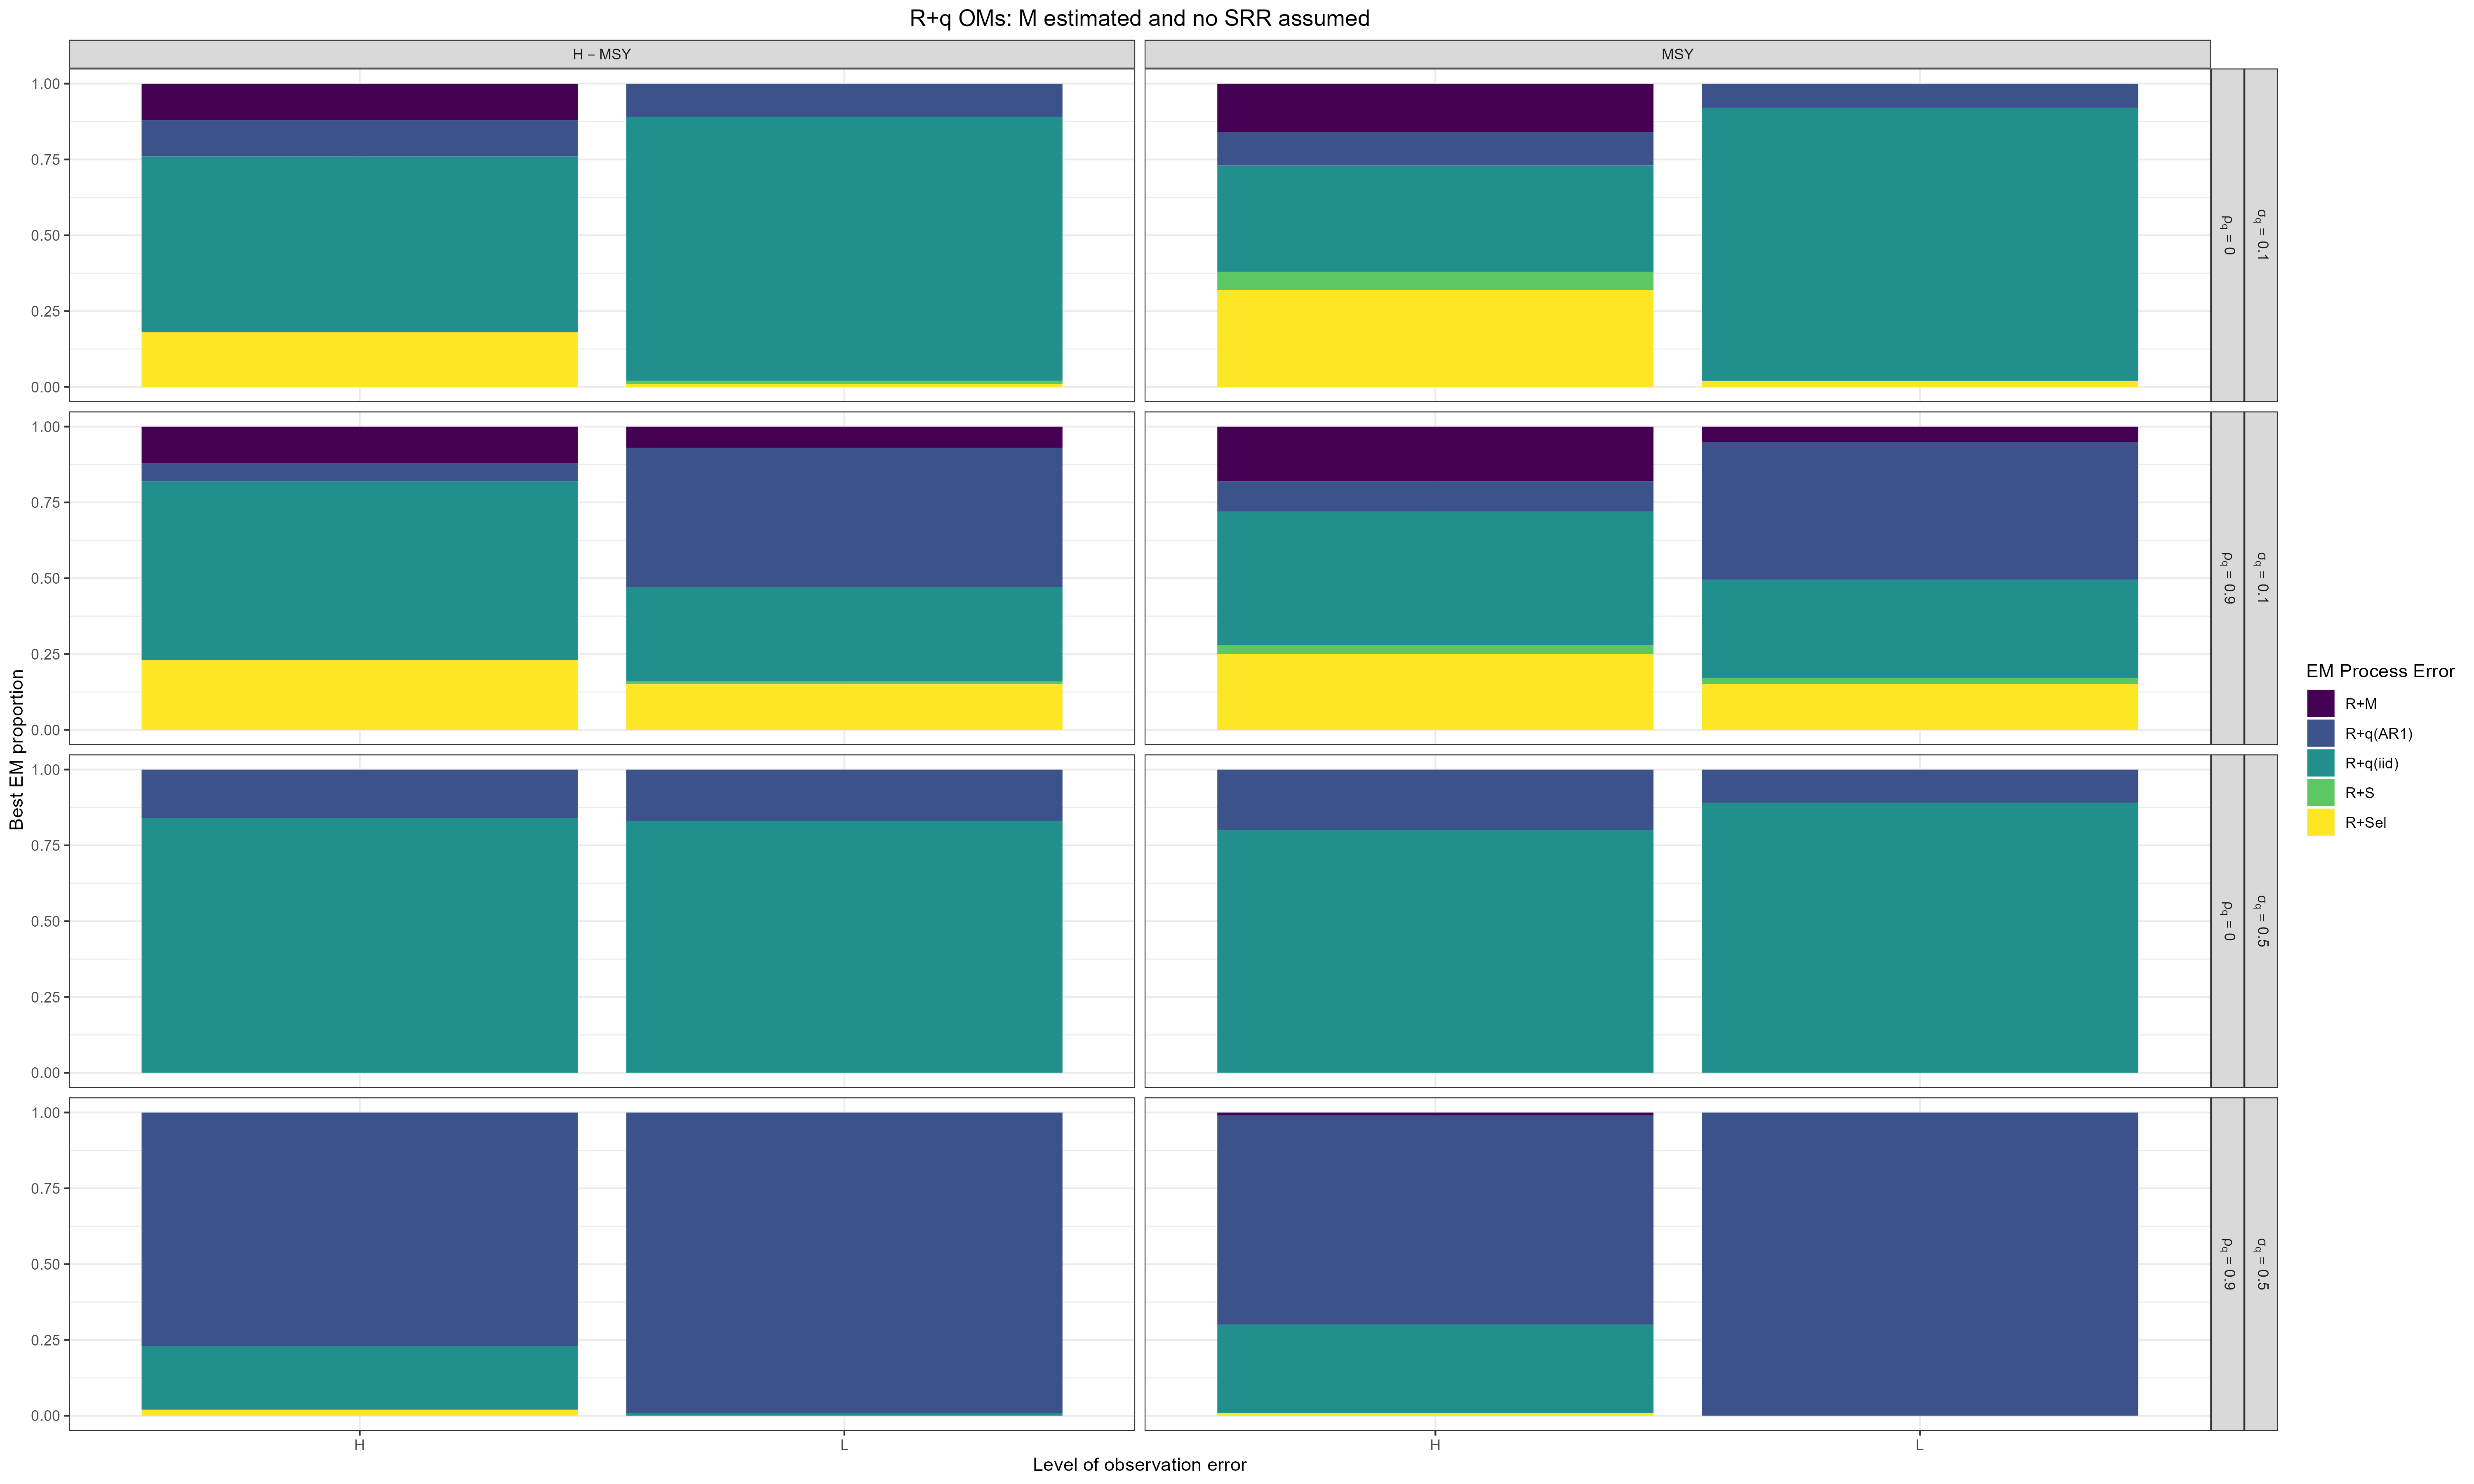
\includegraphics[width = \textwidth]{q_om_proportion_best_aic_R_ME.png}
\end{center}
\end{figure}
\end{landscape}

\begin{landscape}
\begin{figure}
\caption{Proportion of simulated data sets from OMs with R+q process errors where fitted estimating models had lowest marginal AIC. All estimating models estimate a stock-recruit relationship and and M is fixed at the true value.} \label{q_om_proportion_best_aic_SR_MF}
\begin{center}
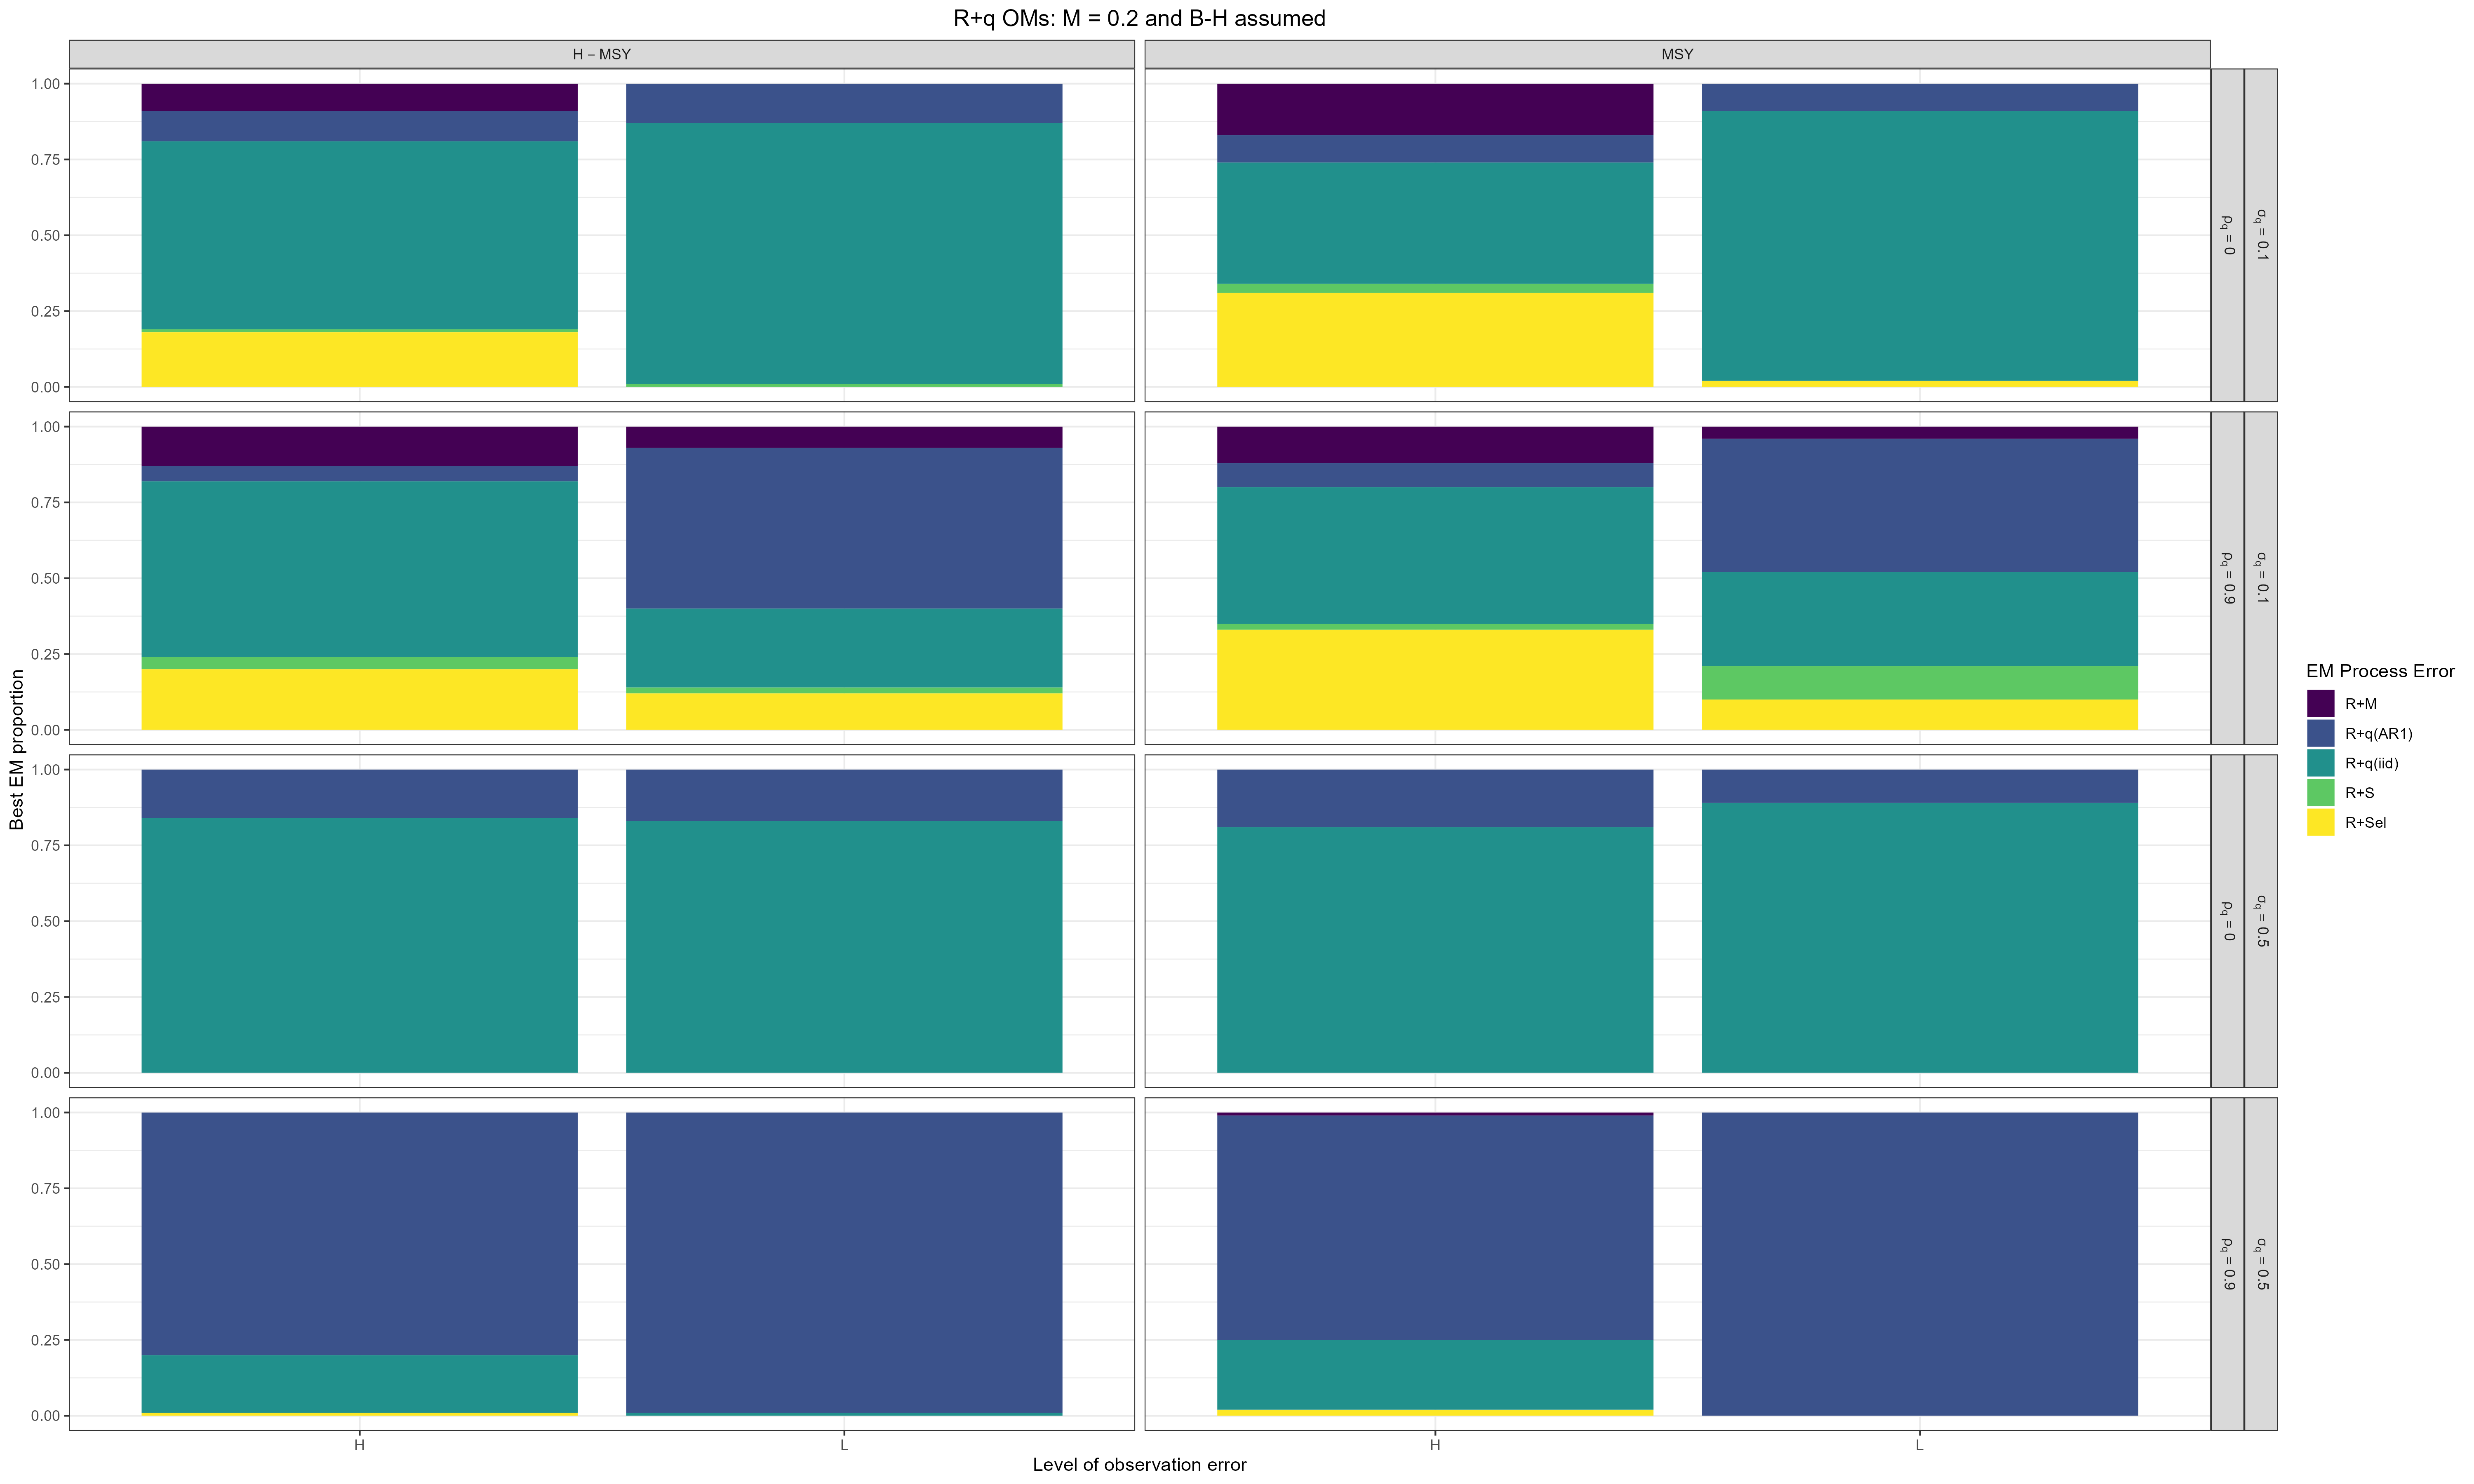
\includegraphics[width = \textwidth]{q_om_proportion_best_aic_SR_MF.png}
\end{center}
\end{figure}
\end{landscape}

\begin{landscape}
\begin{figure}
\caption{Proportion of simulated data sets from OMs with R+q process errors where fitted estimating models had lowest marginal AIC. All estimating models estimate a stock-recruit relationship and and M is estimated.} \label{q_om_proportion_best_aic_SR_ME}
\begin{center}
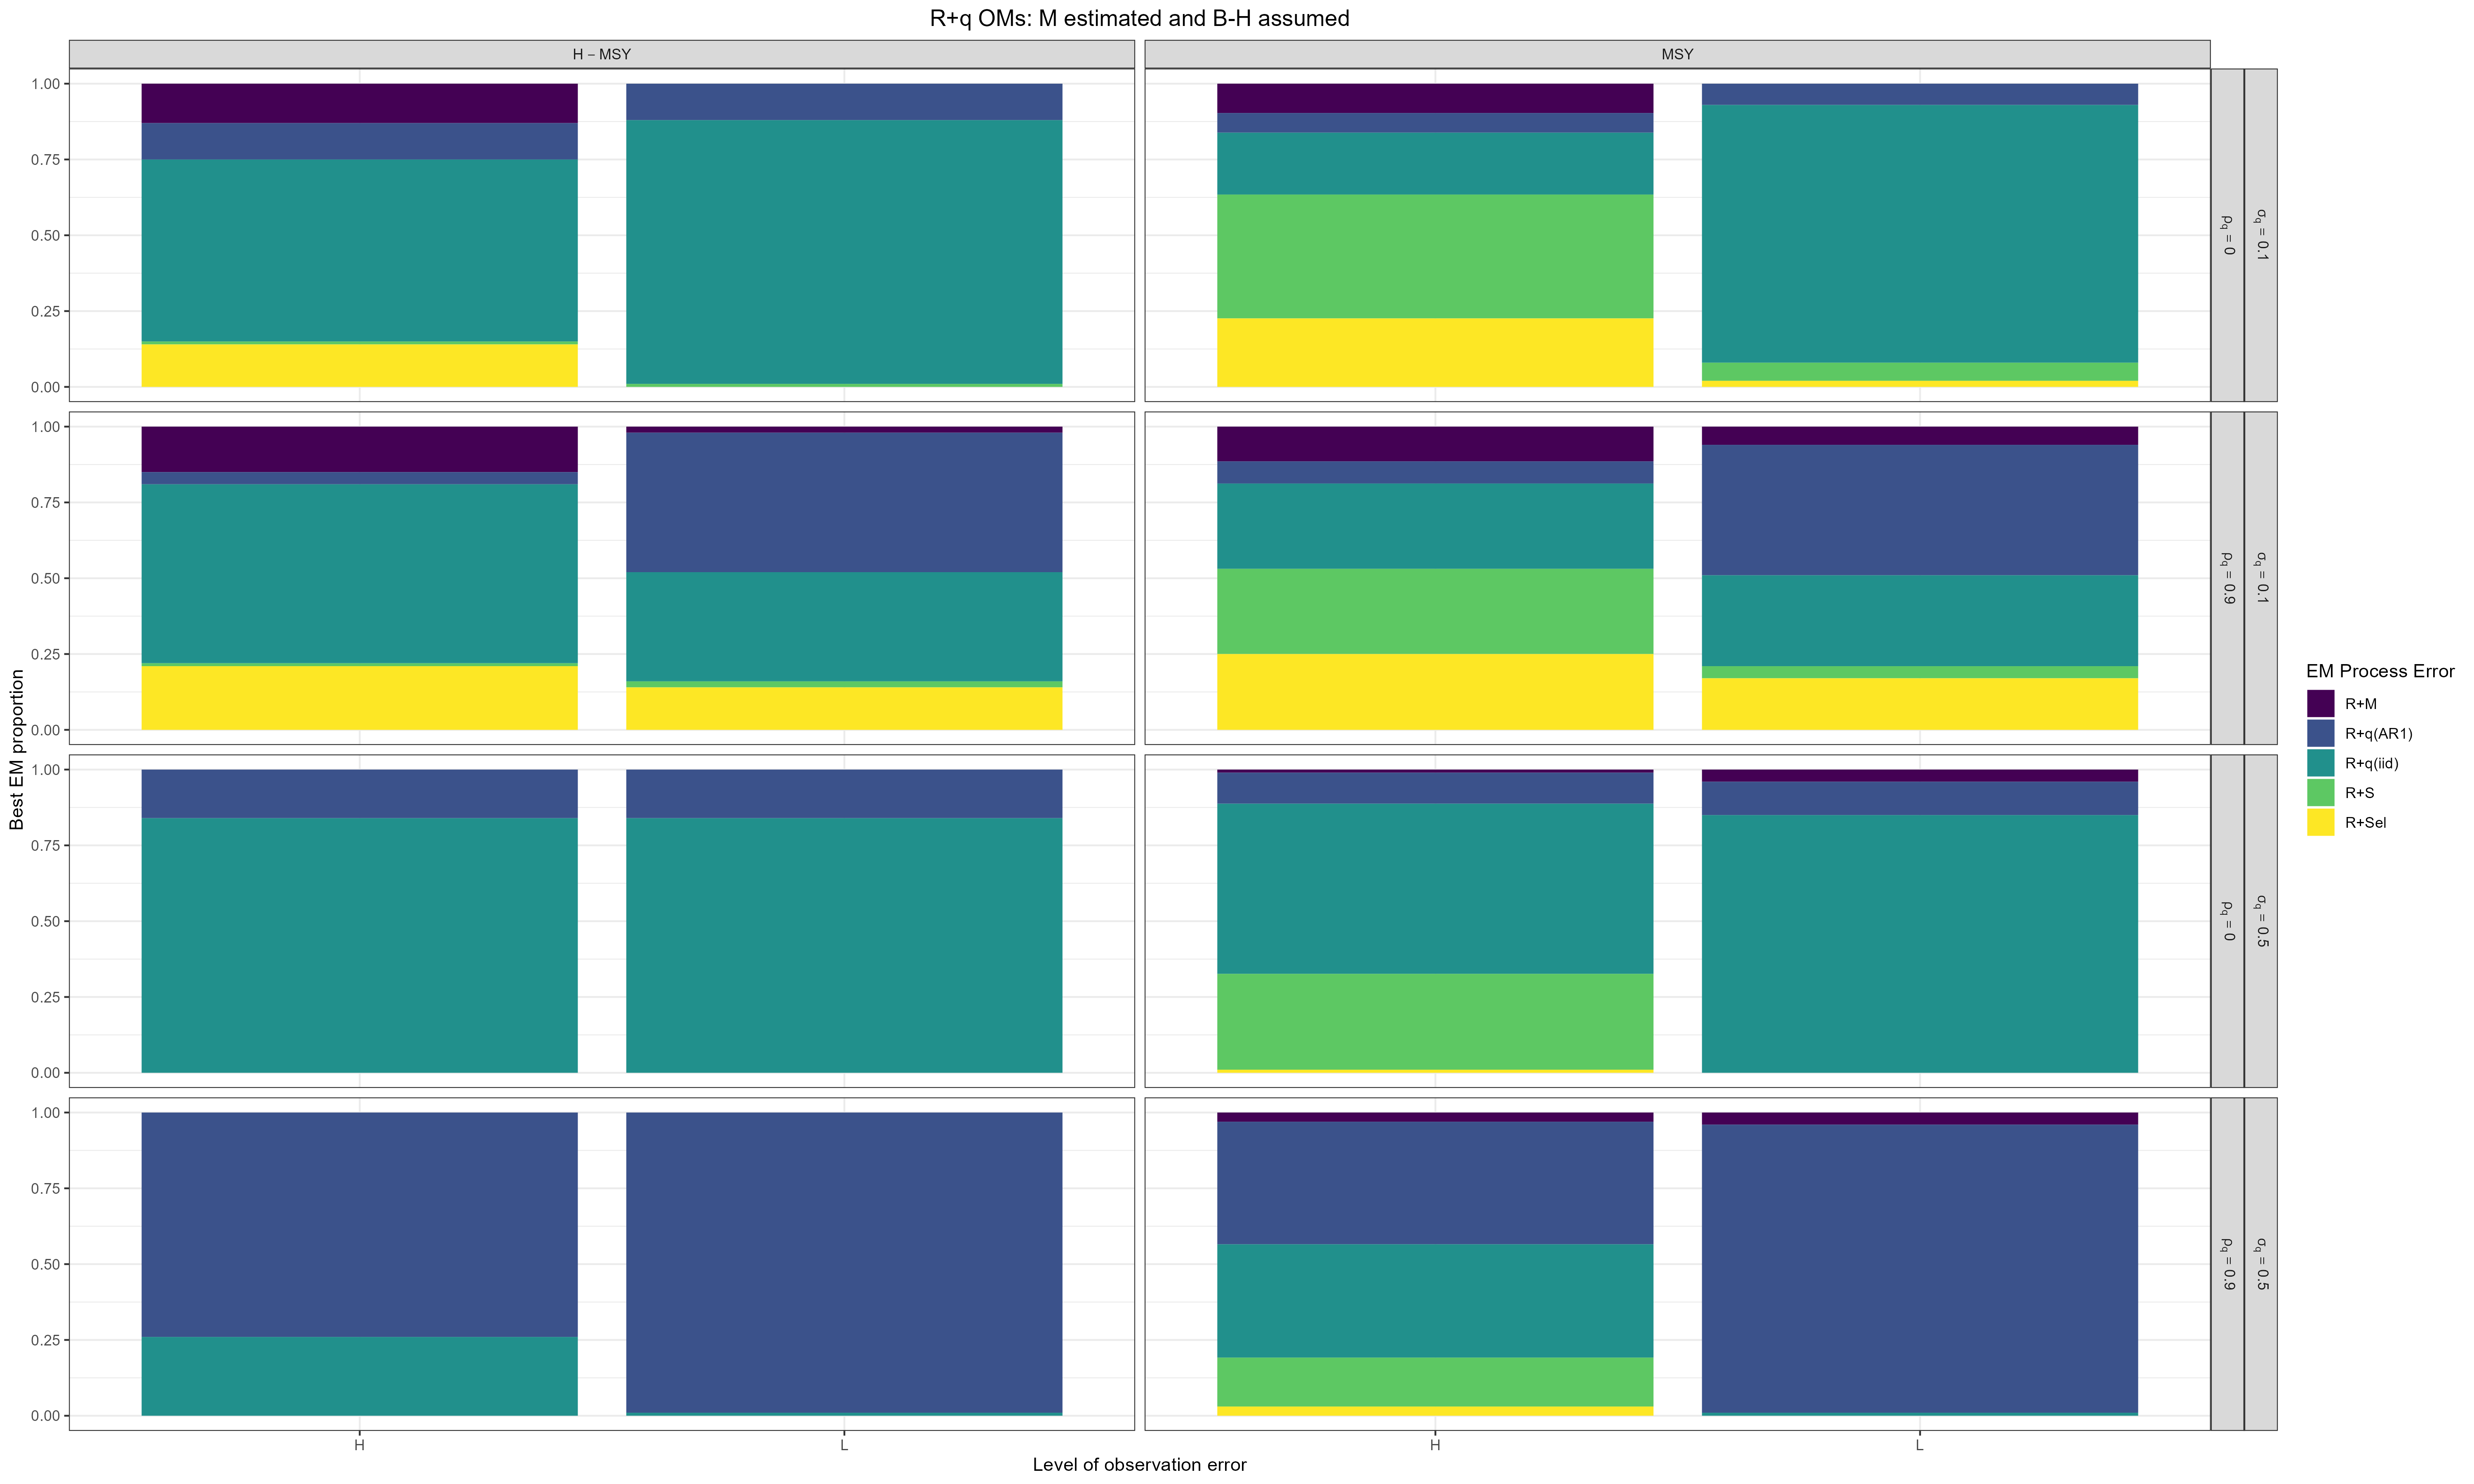
\includegraphics[width = \textwidth]{q_om_proportion_best_aic_SR_ME.png}
\end{center}
\end{figure}
\end{landscape}

\clearpage

\begin{figure}
\caption{Predicted probability of AIC preferring BH model as a function of the variation of population SSB. Operating and estimating models have matching R or R+S process error structures. Estimating models assume mean M is fixed at the true value.}\label{naa_om_MF_BH_glm_AIC_plots}
\begin{center}
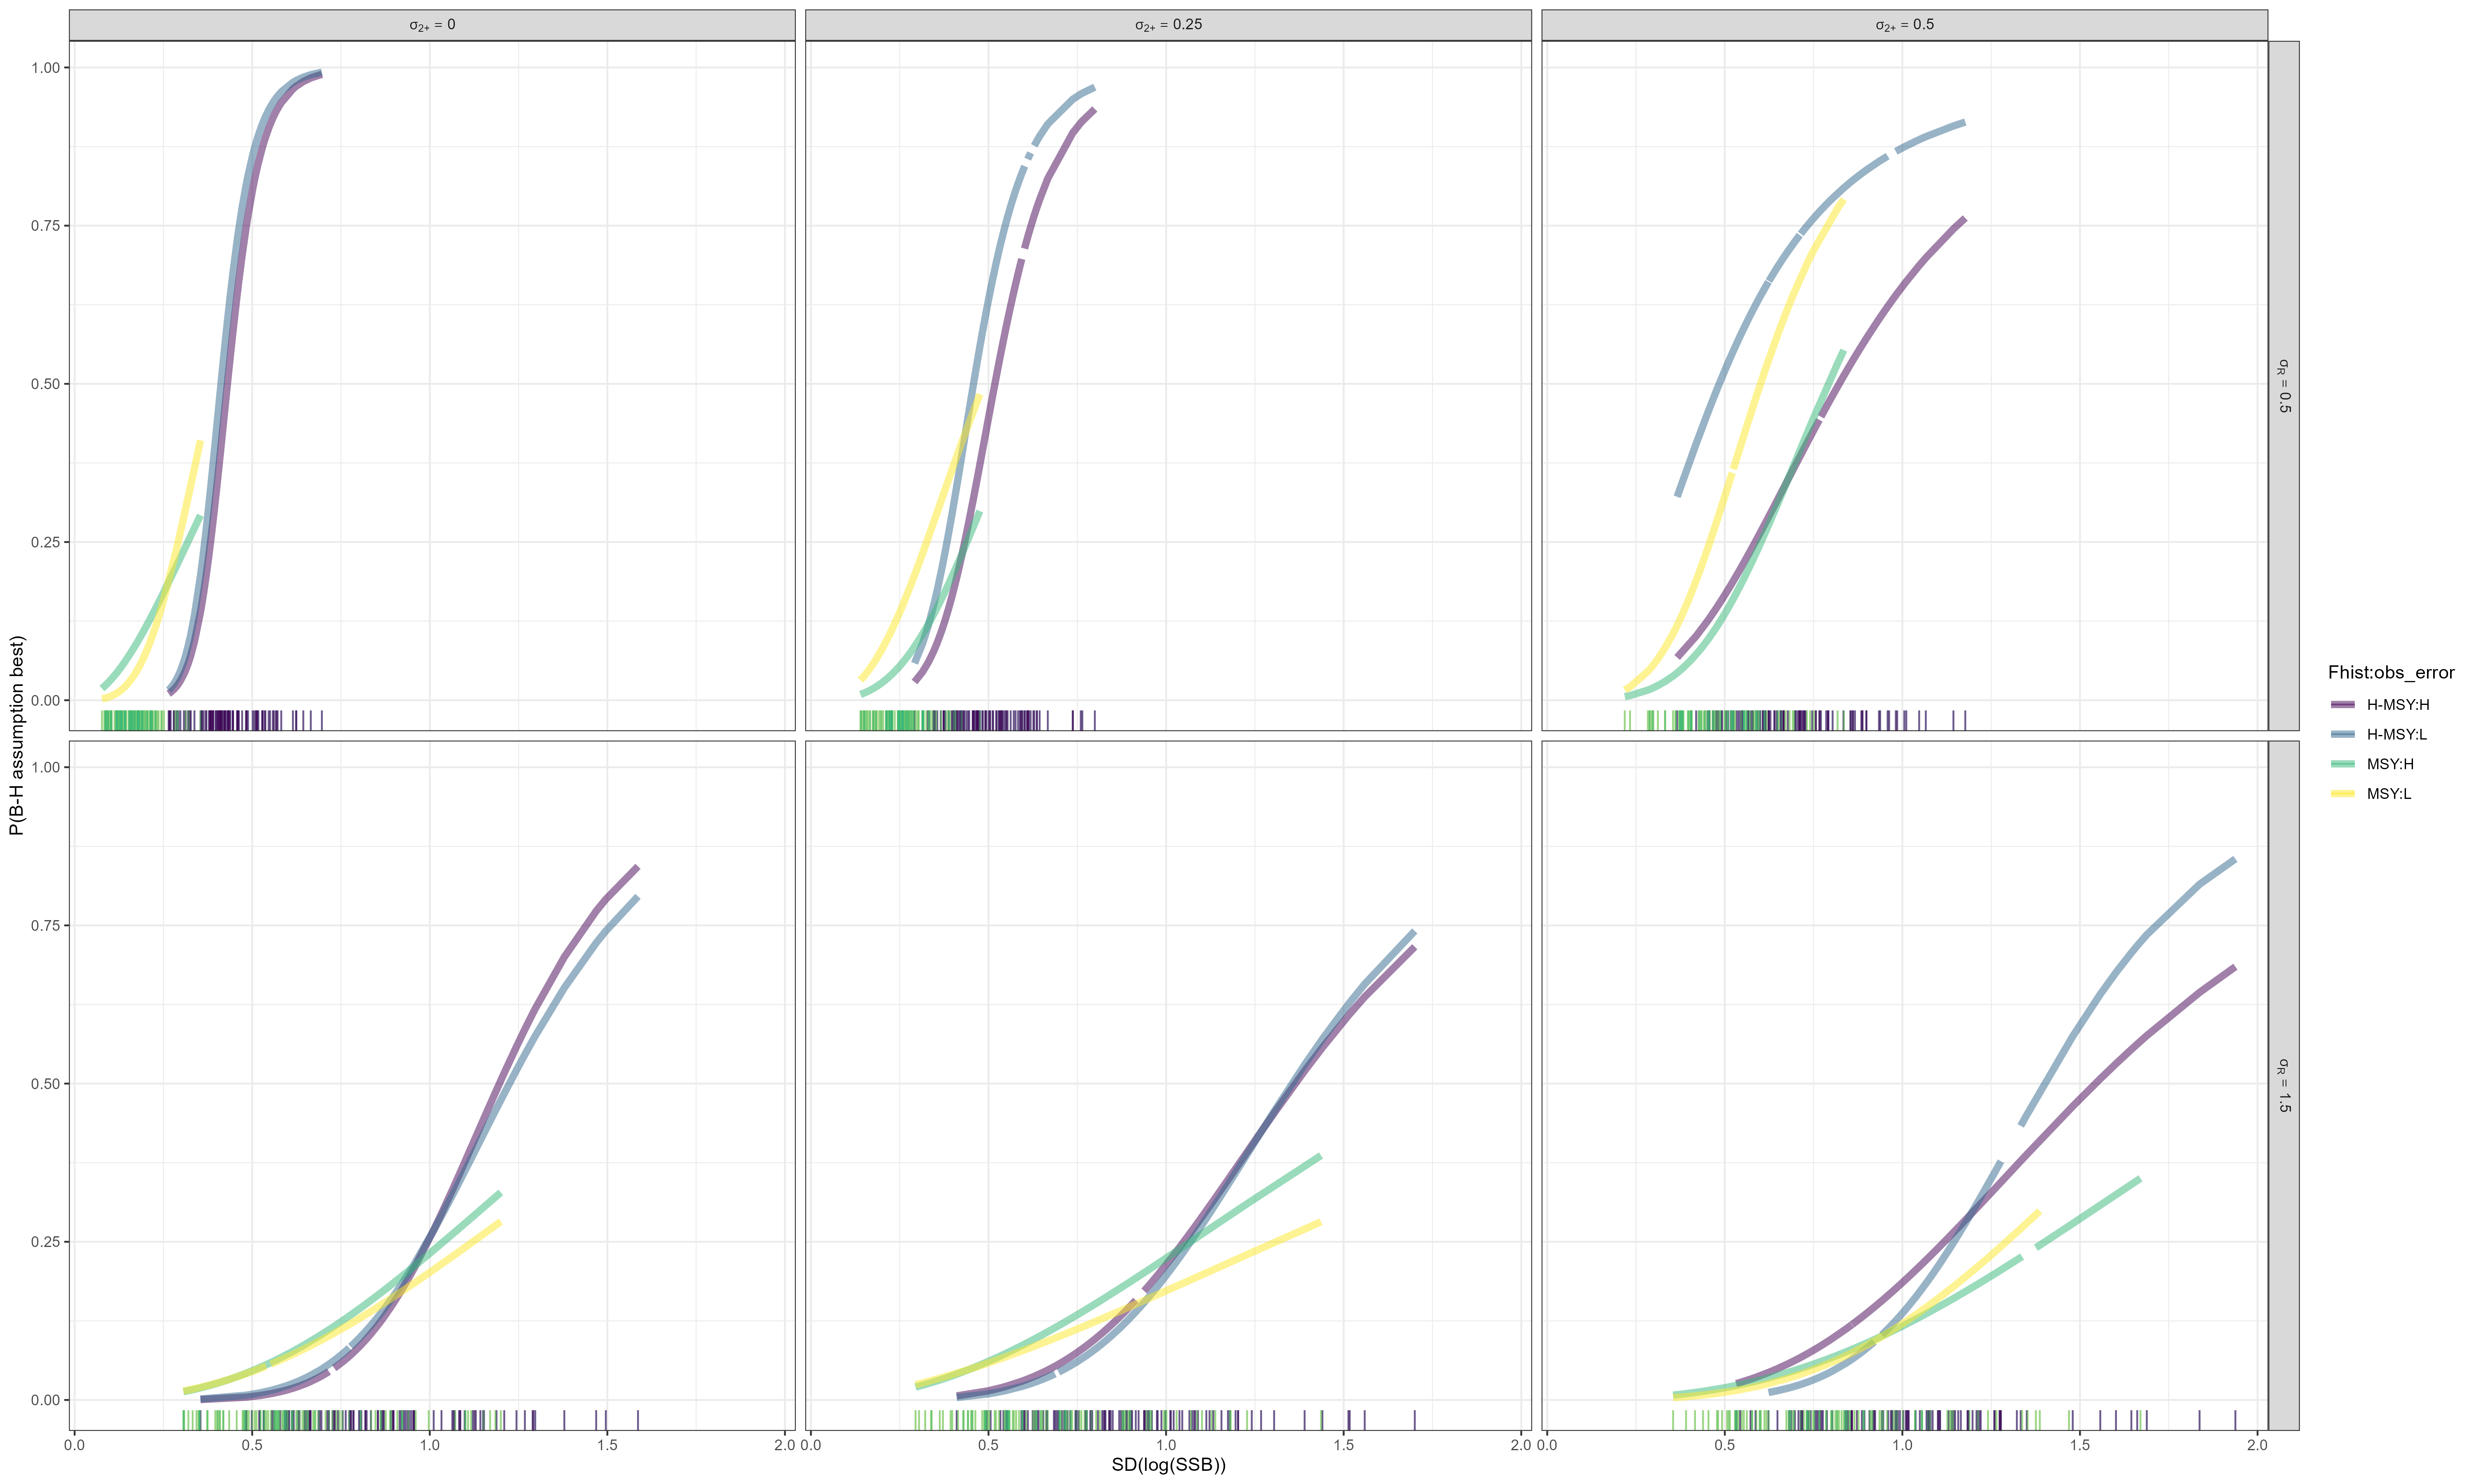
\includegraphics[width = \textwidth]{naa_om_MF_pred_BH_best.png}
\end{center}
\end{figure}

\begin{figure}
\caption{Predicted probability of AIC preferring BH model as a function of the variation of population SSB. Operating and estimating models have matching R or R+S process error structures. Estimating models allow estimation of mean M.}\label{naa_om_ME_BH_glm_AIC_plots}
\begin{center}
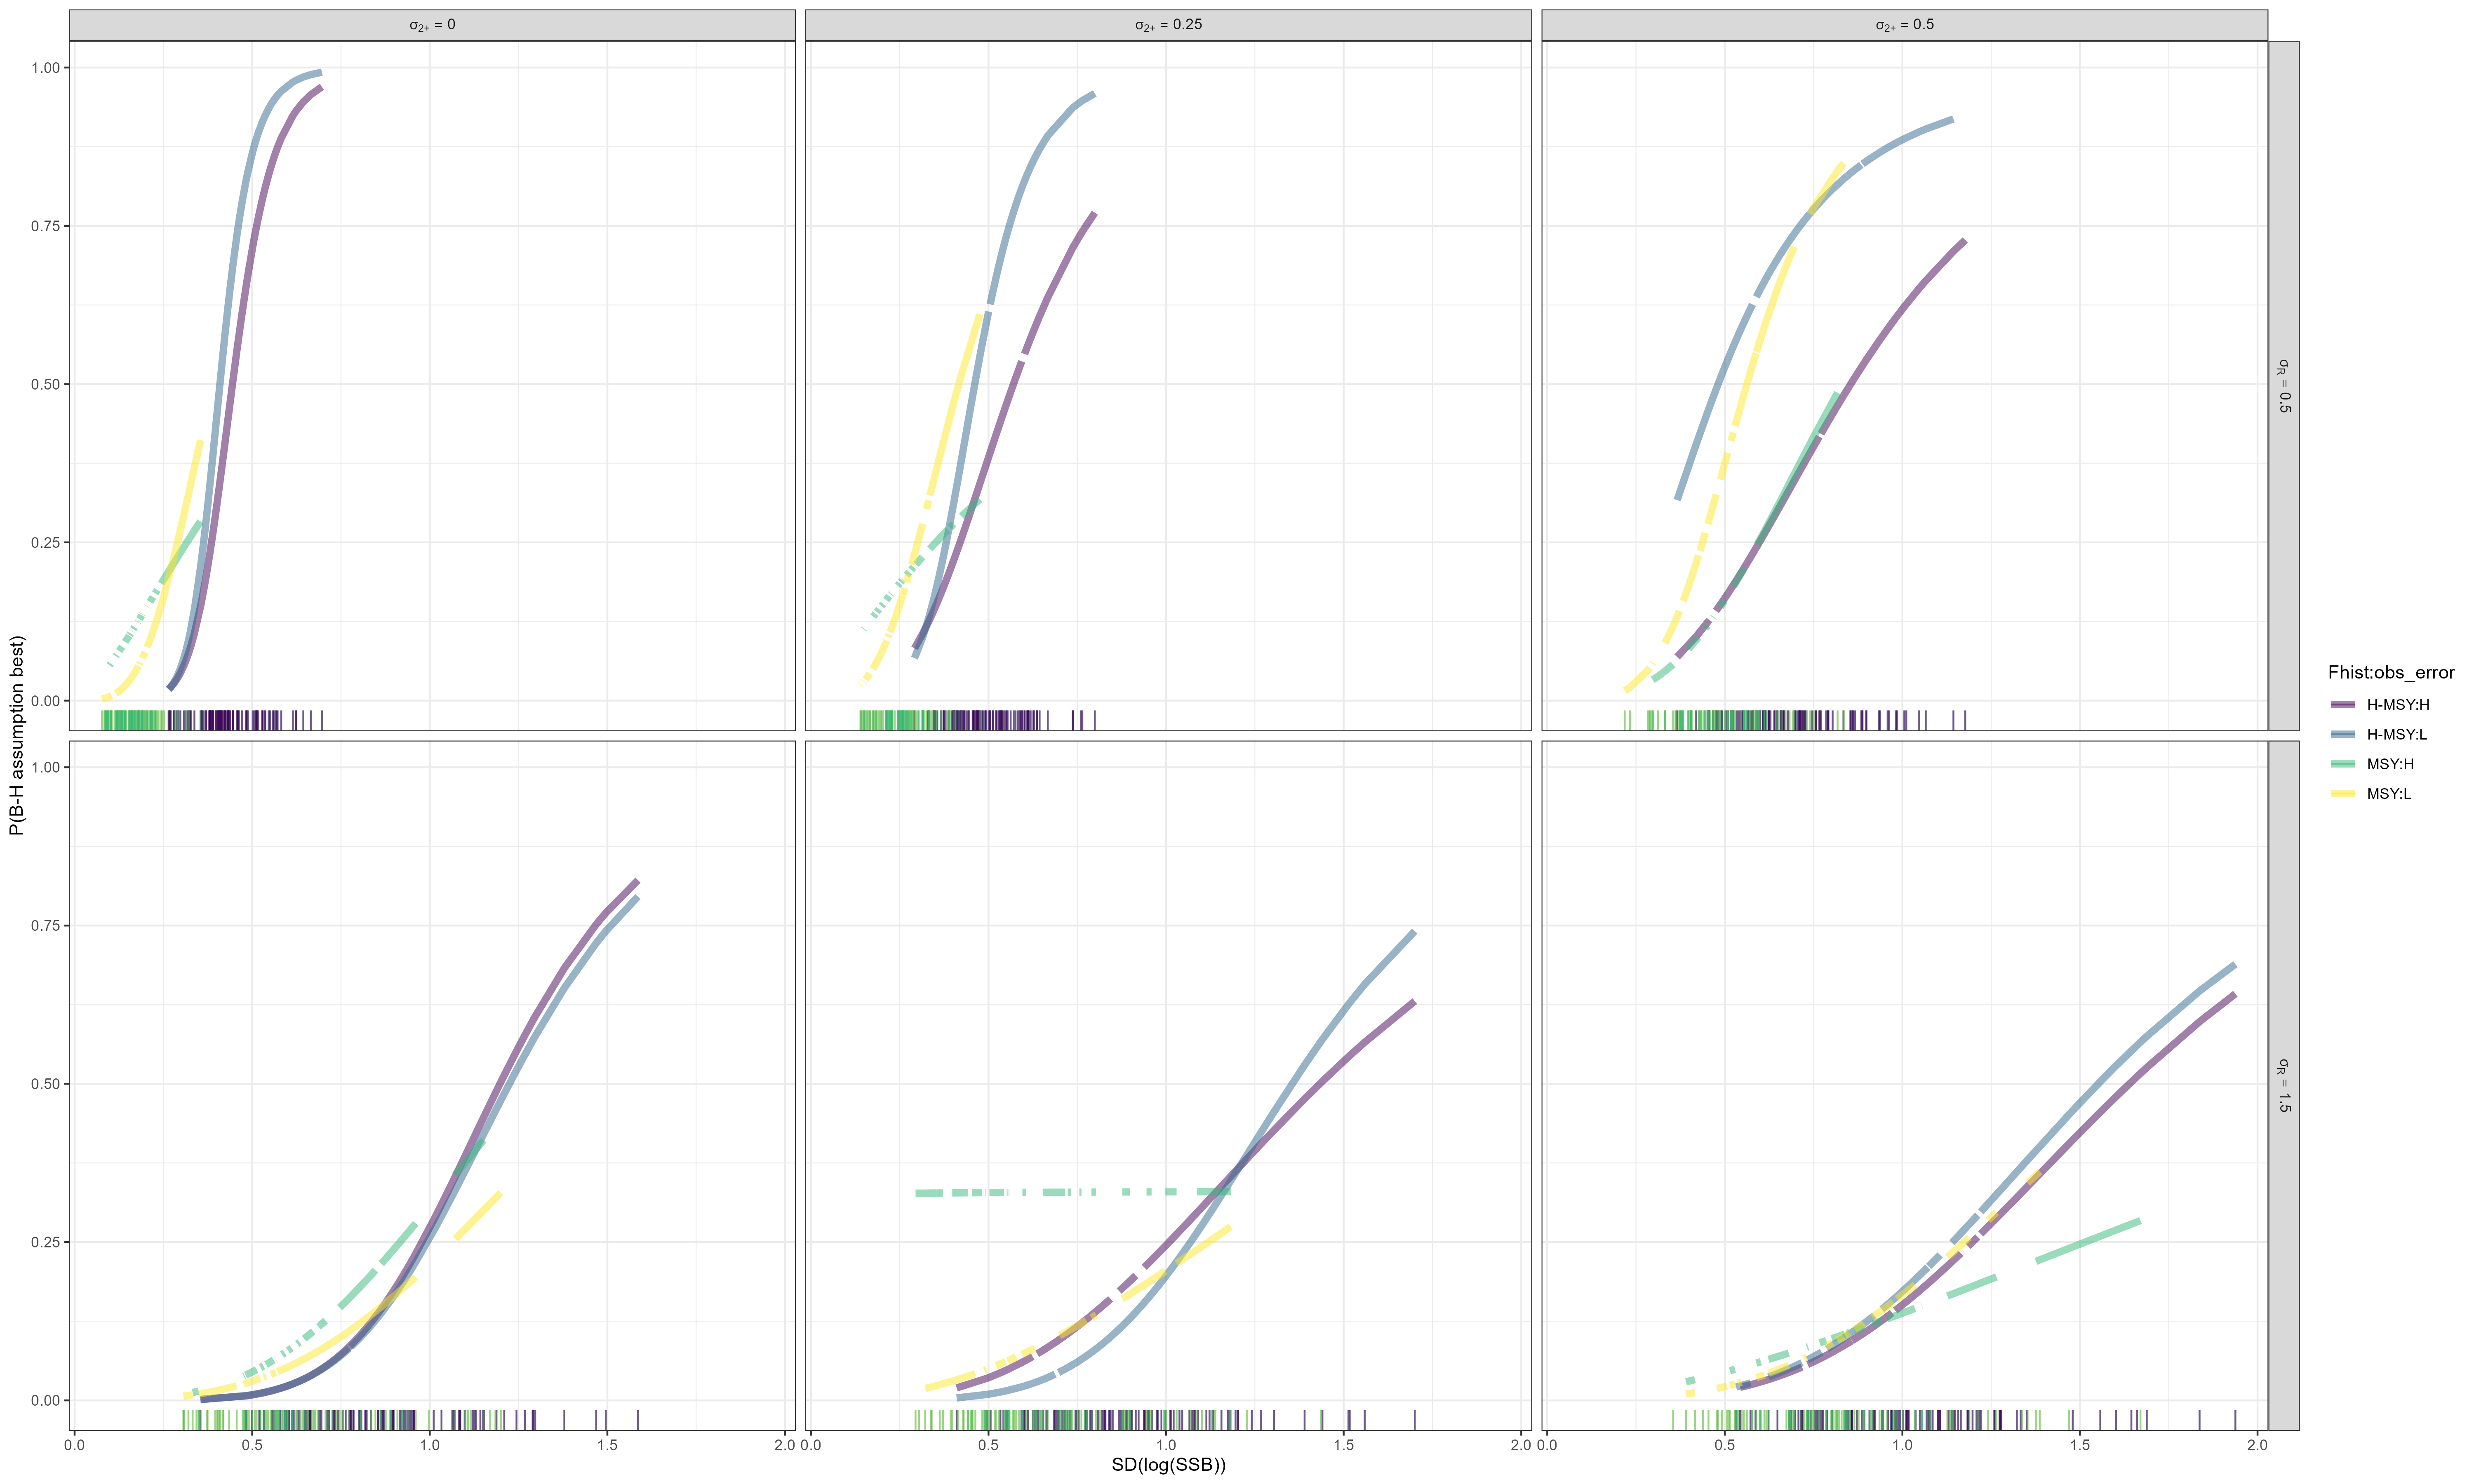
\includegraphics[width = \textwidth]{naa_om_ME_pred_BH_best.png}
\end{center}
\end{figure}

\begin{figure}
\caption{Predicted probability of AIC preferring BH model as a function of the variation of population SSB. Operating and estimating models have matching R+M process error structures. Estimating models assume mean M is fixed at the true value.}\label{M_om_MF_BH_glm_AIC_plots}
\begin{center}
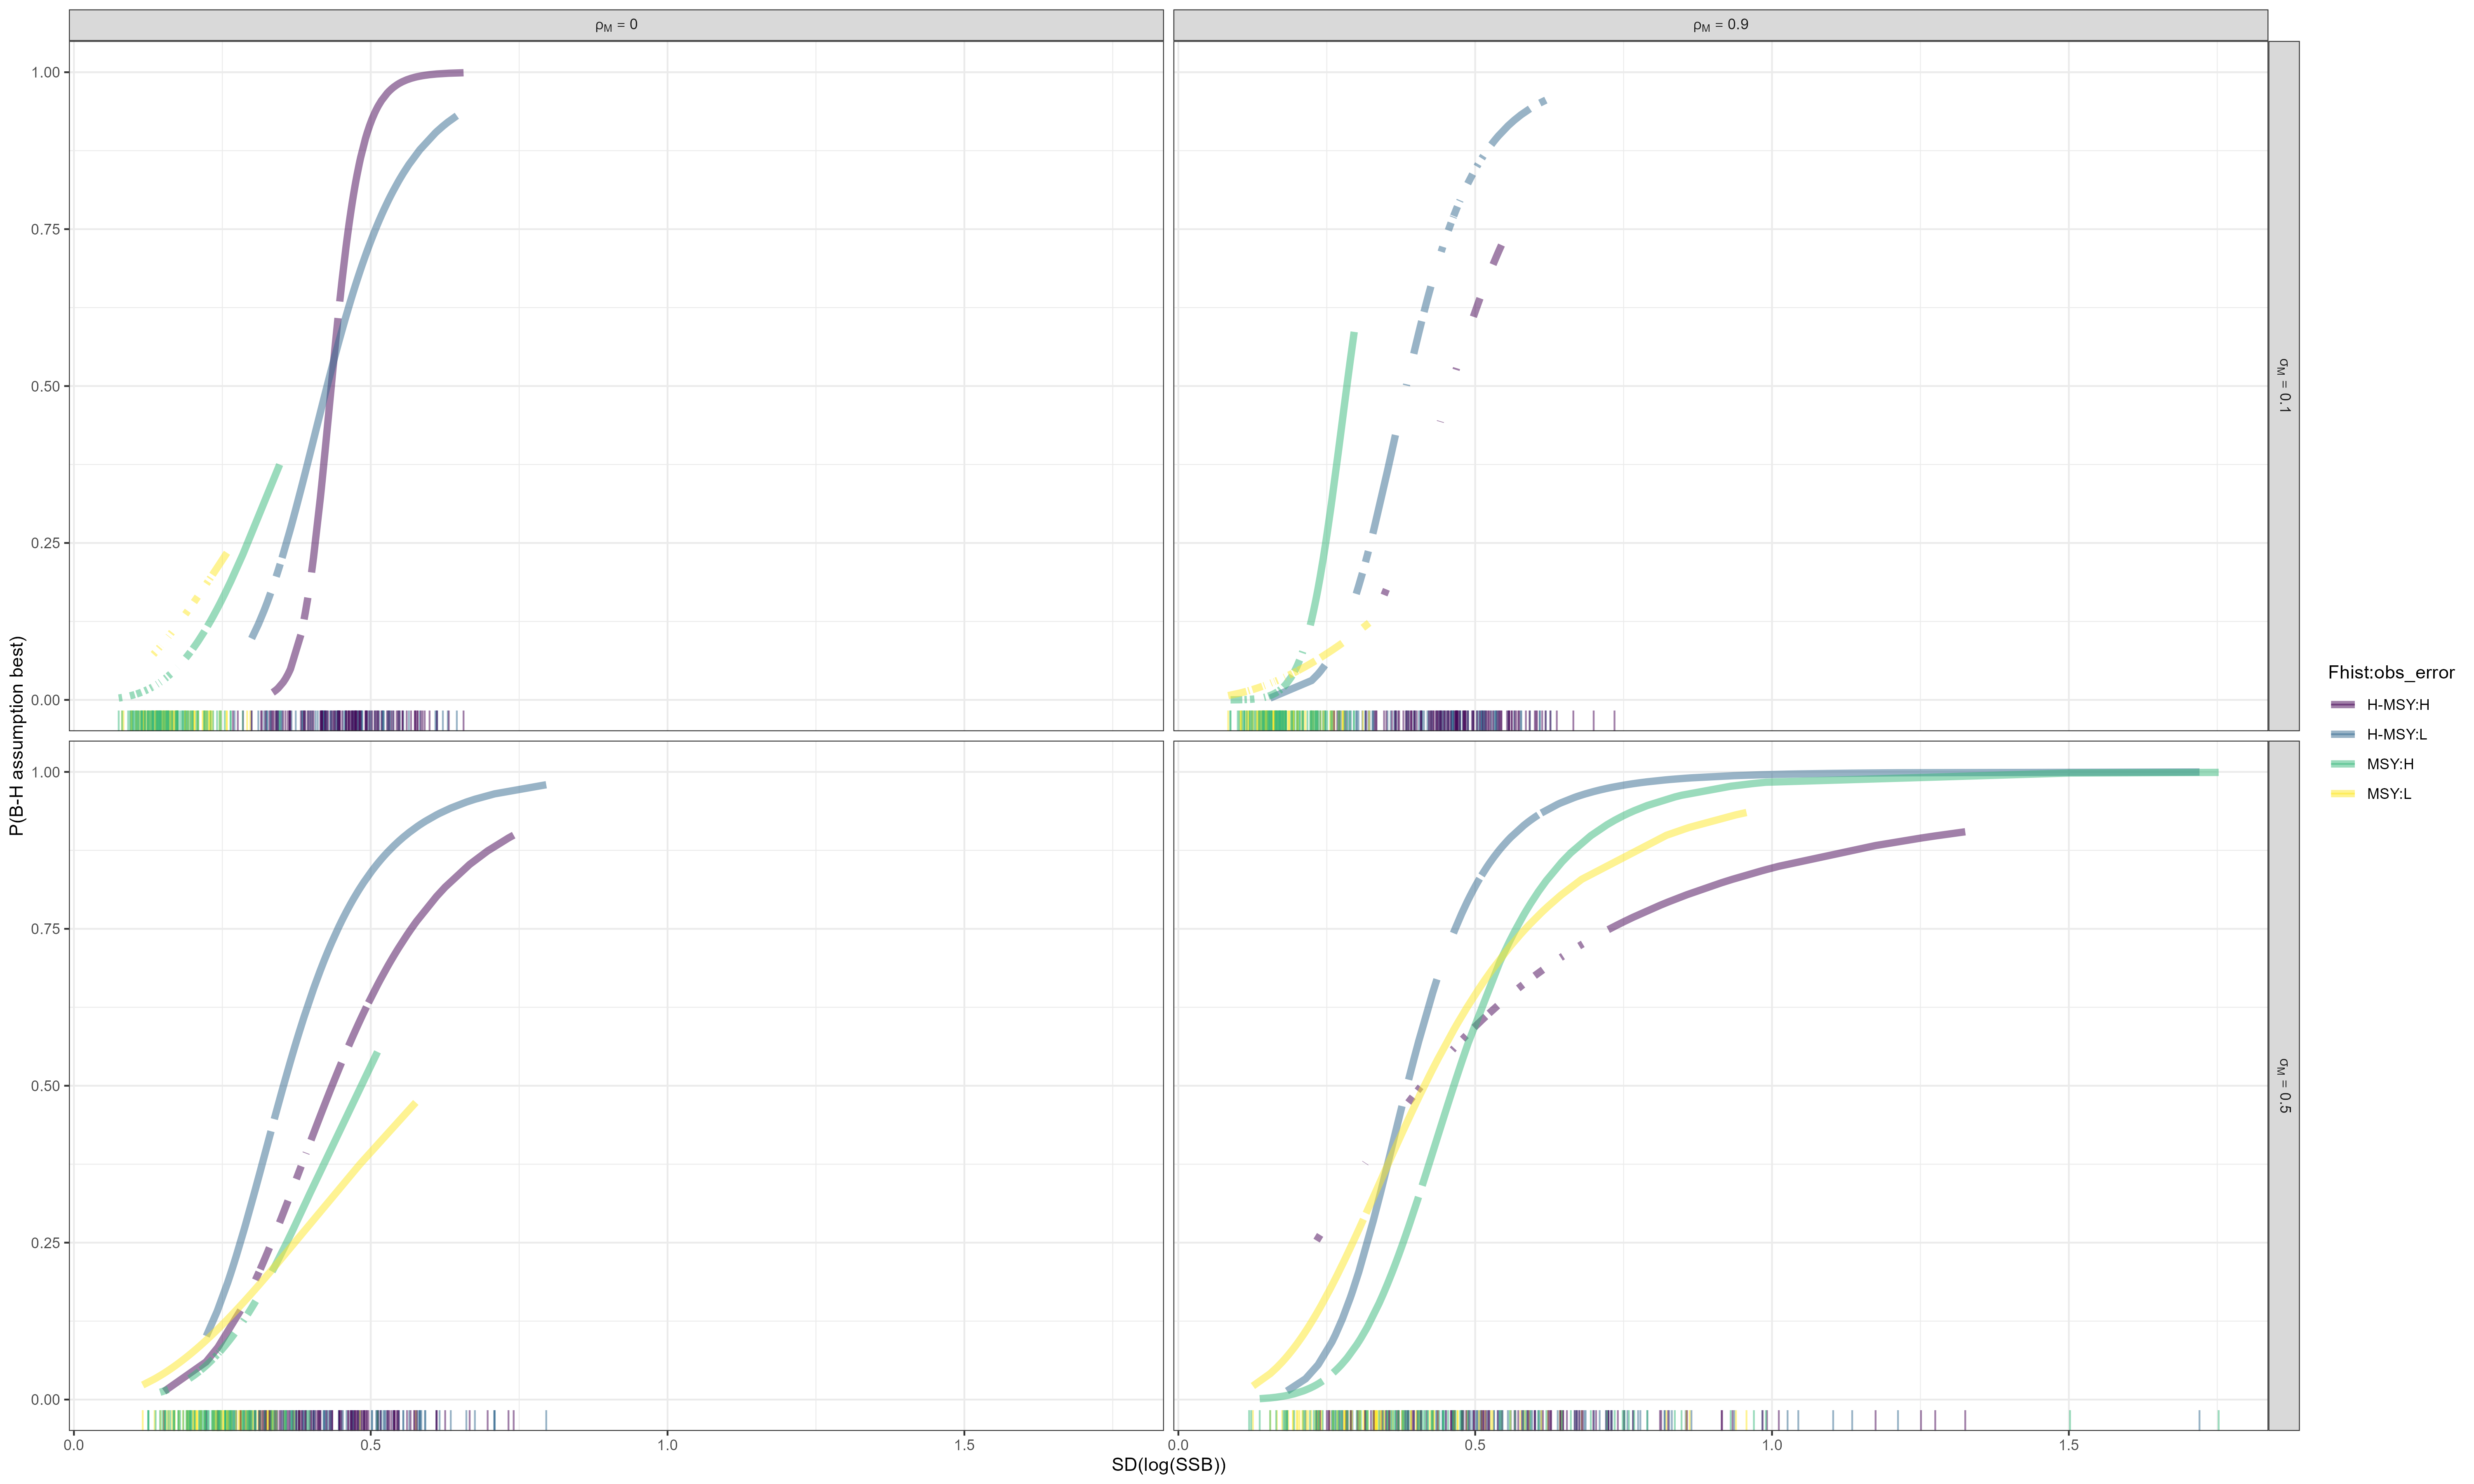
\includegraphics[width = \textwidth]{M_om_MF_pred_BH_best.png}
\end{center}
\end{figure}

\begin{figure}
\caption{Predicted probability of AIC preferring BH model as a function of the variation of population SSB. Operating and estimating models have matching R+M process error structures. Estimating models allow estimation of mean M.}\label{M_om_ME_BH_glm_AIC_plots}
\begin{center}
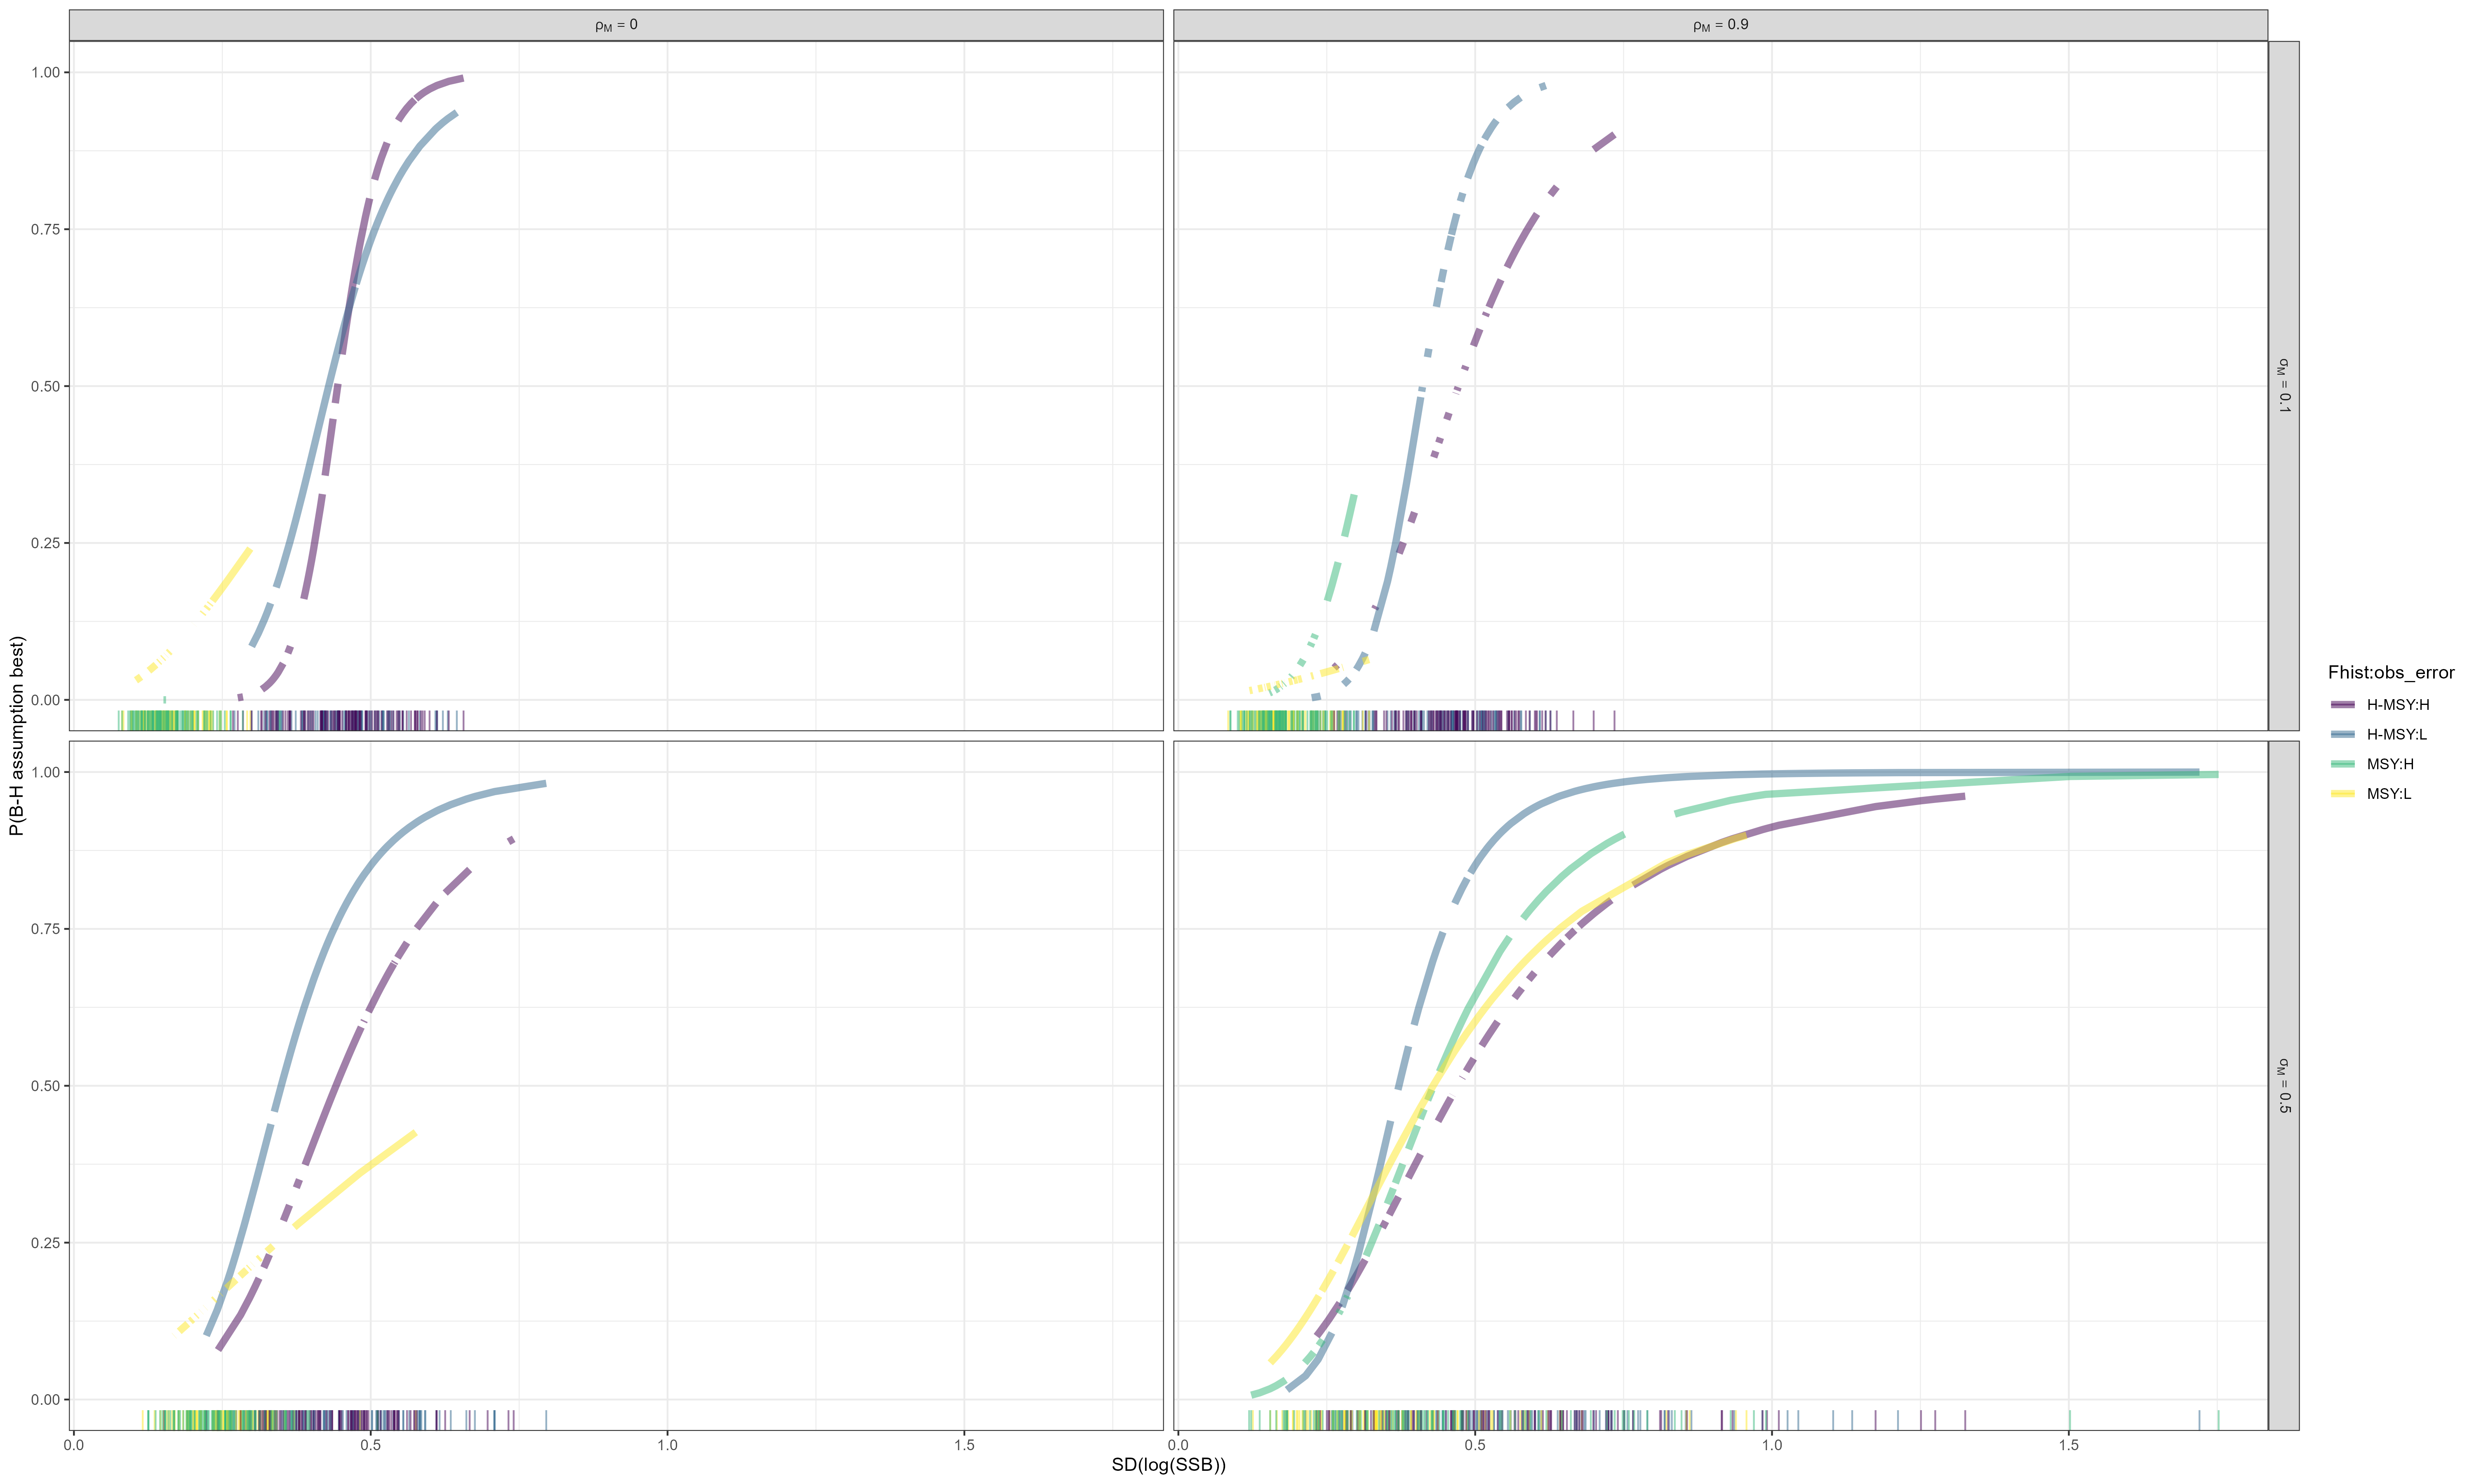
\includegraphics[width = \textwidth]{M_om_ME_pred_BH_best.png}
\end{center}
\end{figure}

\begin{figure}
\caption{Predicted probability of AIC preferring BH model as a function of the variation of population SSB. Operating and estimating models have matching R+Sel process error structures. Estimating models assume mean M is fixed at the true value.}\label{Sel_om_MF_BH_glm_AIC_plots}
\begin{center}
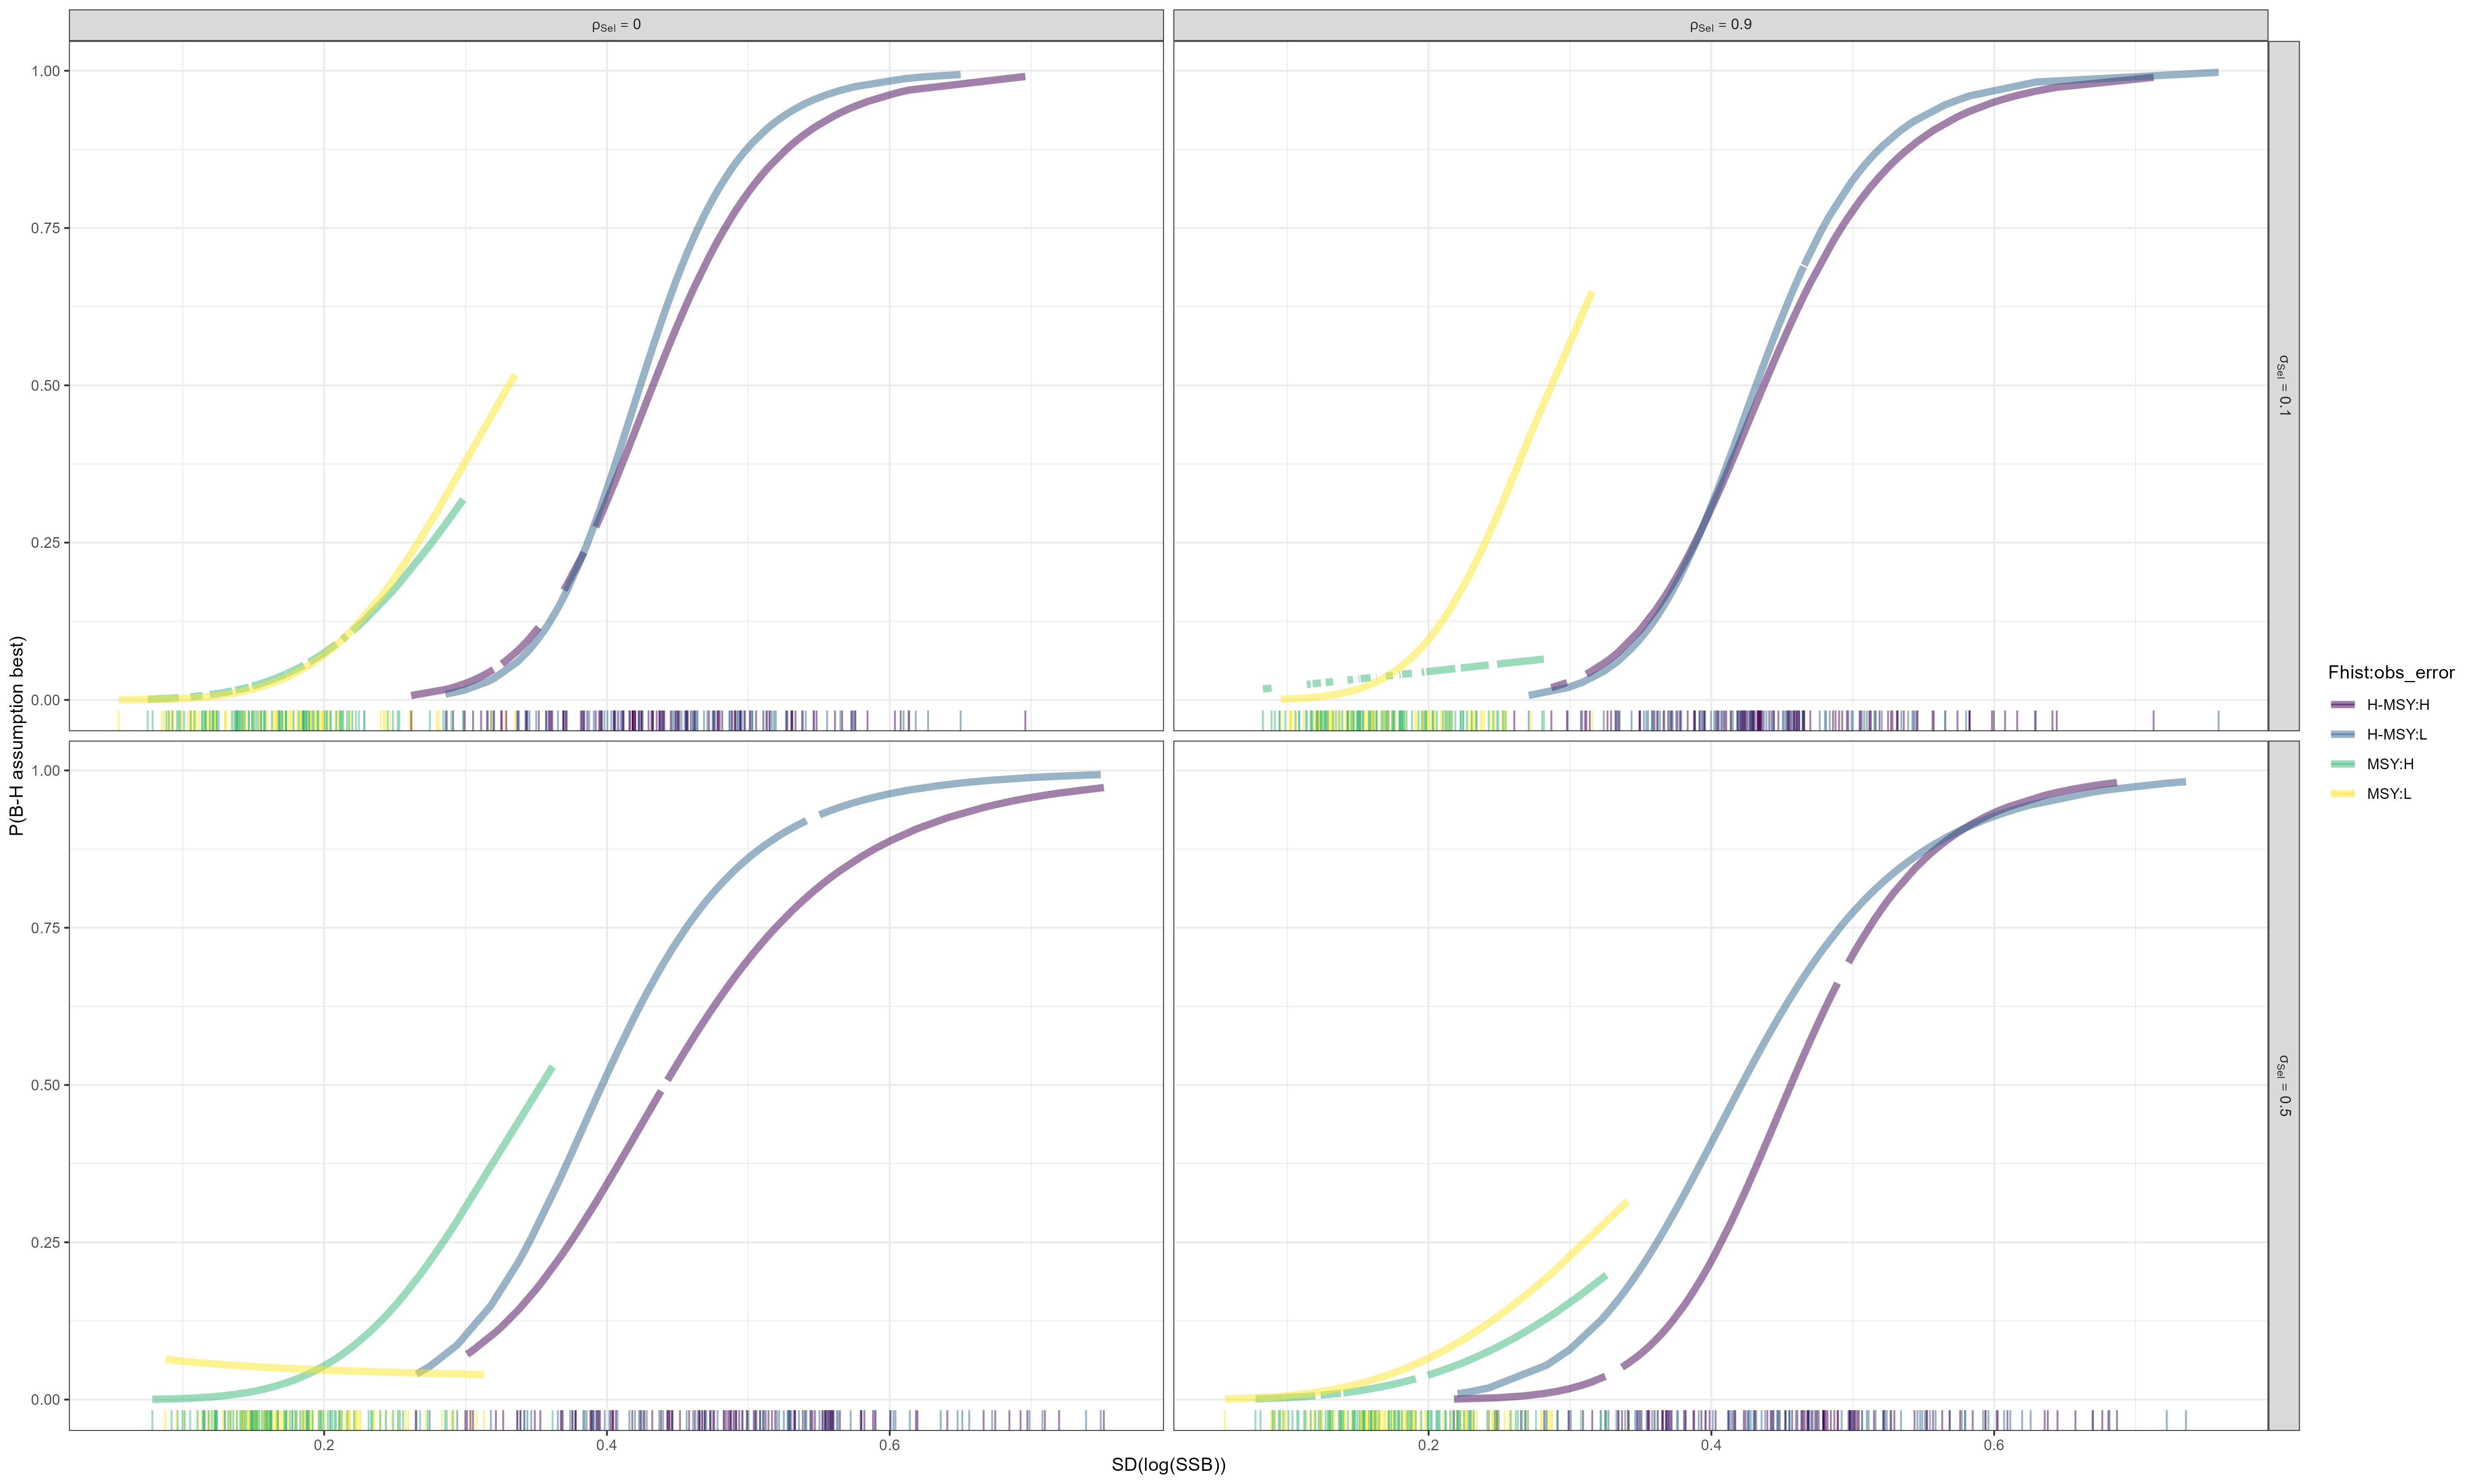
\includegraphics[width = \textwidth]{Sel_om_MF_pred_BH_best.png}
\end{center}
\end{figure}

\begin{figure}
\caption{Predicted probability of AIC preferring BH model as a function of the variation of population SSB. Operating and estimating models have matching R+Sel process error structures. Estimating models allow estimation of mean M.}\label{Sel_om_ME_BH_glm_AIC_plots}
\begin{center}
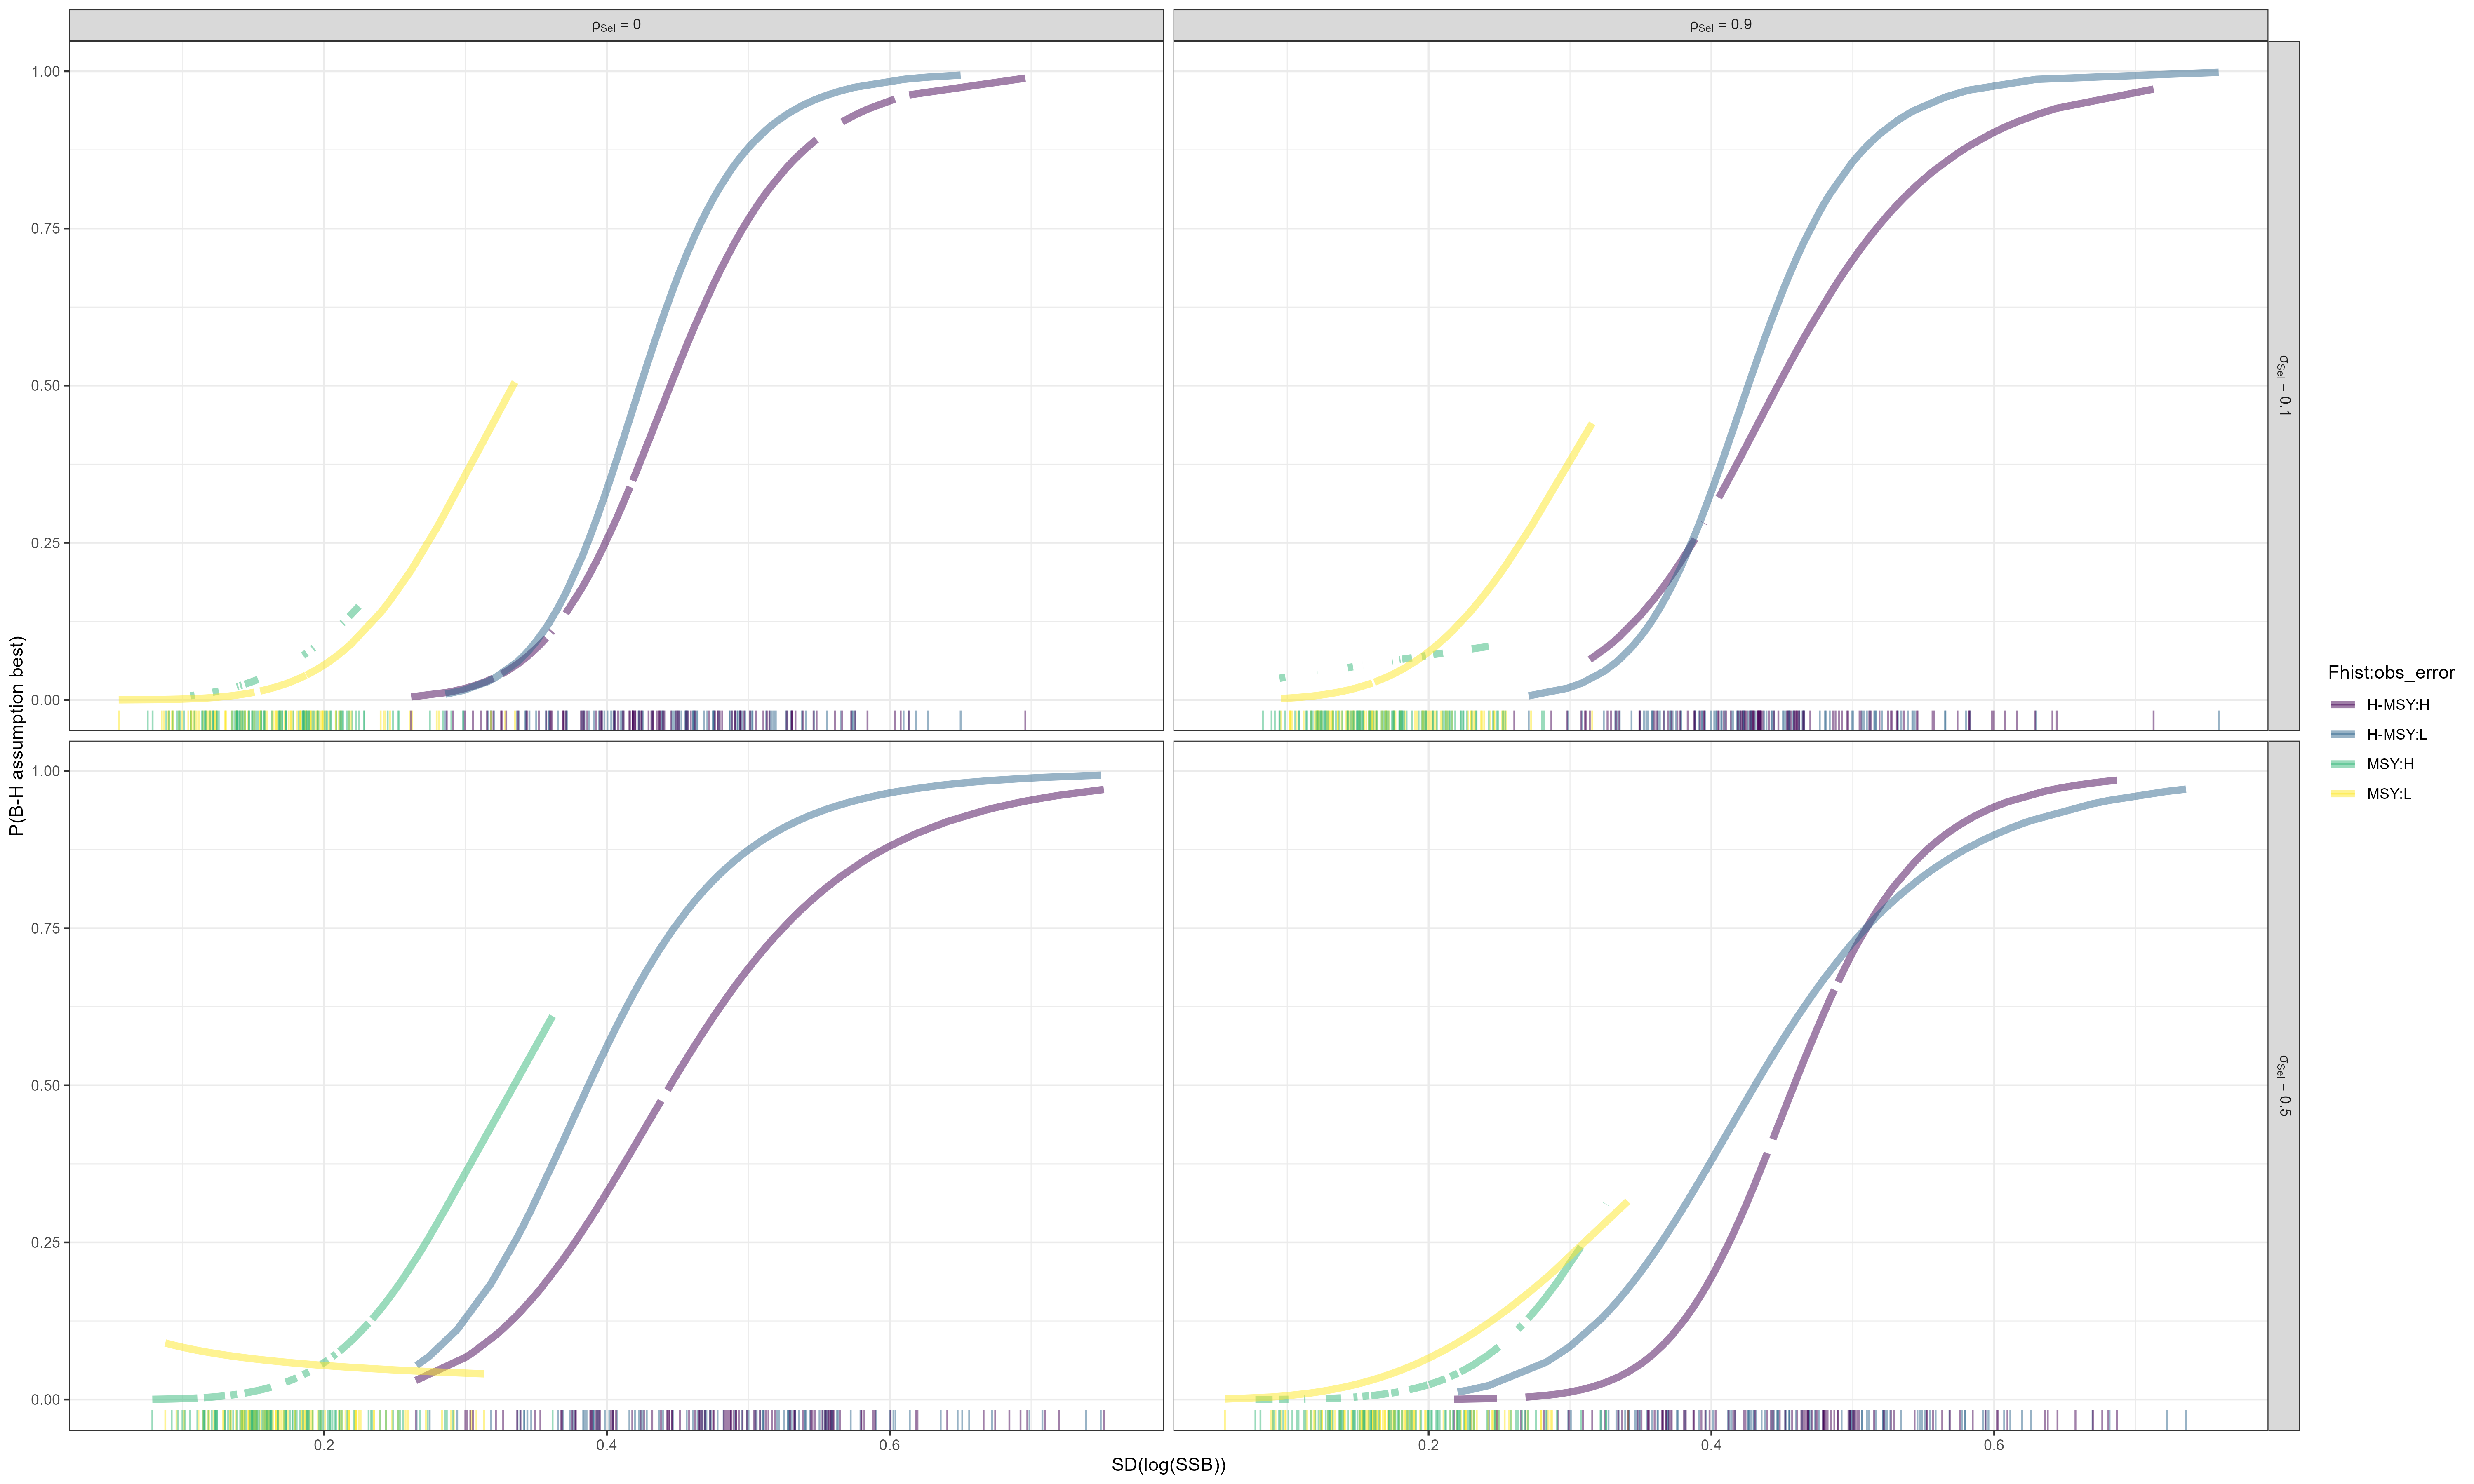
\includegraphics[width = \textwidth]{Sel_om_ME_pred_BH_best.png}
\end{center}
\end{figure}

\begin{figure}
\caption{Predicted probability of AIC preferring BH model as a function of the variation of population SSB. Operating and estimating models have matching R+q process error structures. Estimating models assume mean M is fixed at the true value.}\label{q_om_MF_BH_glm_AIC_plots}
\begin{center}
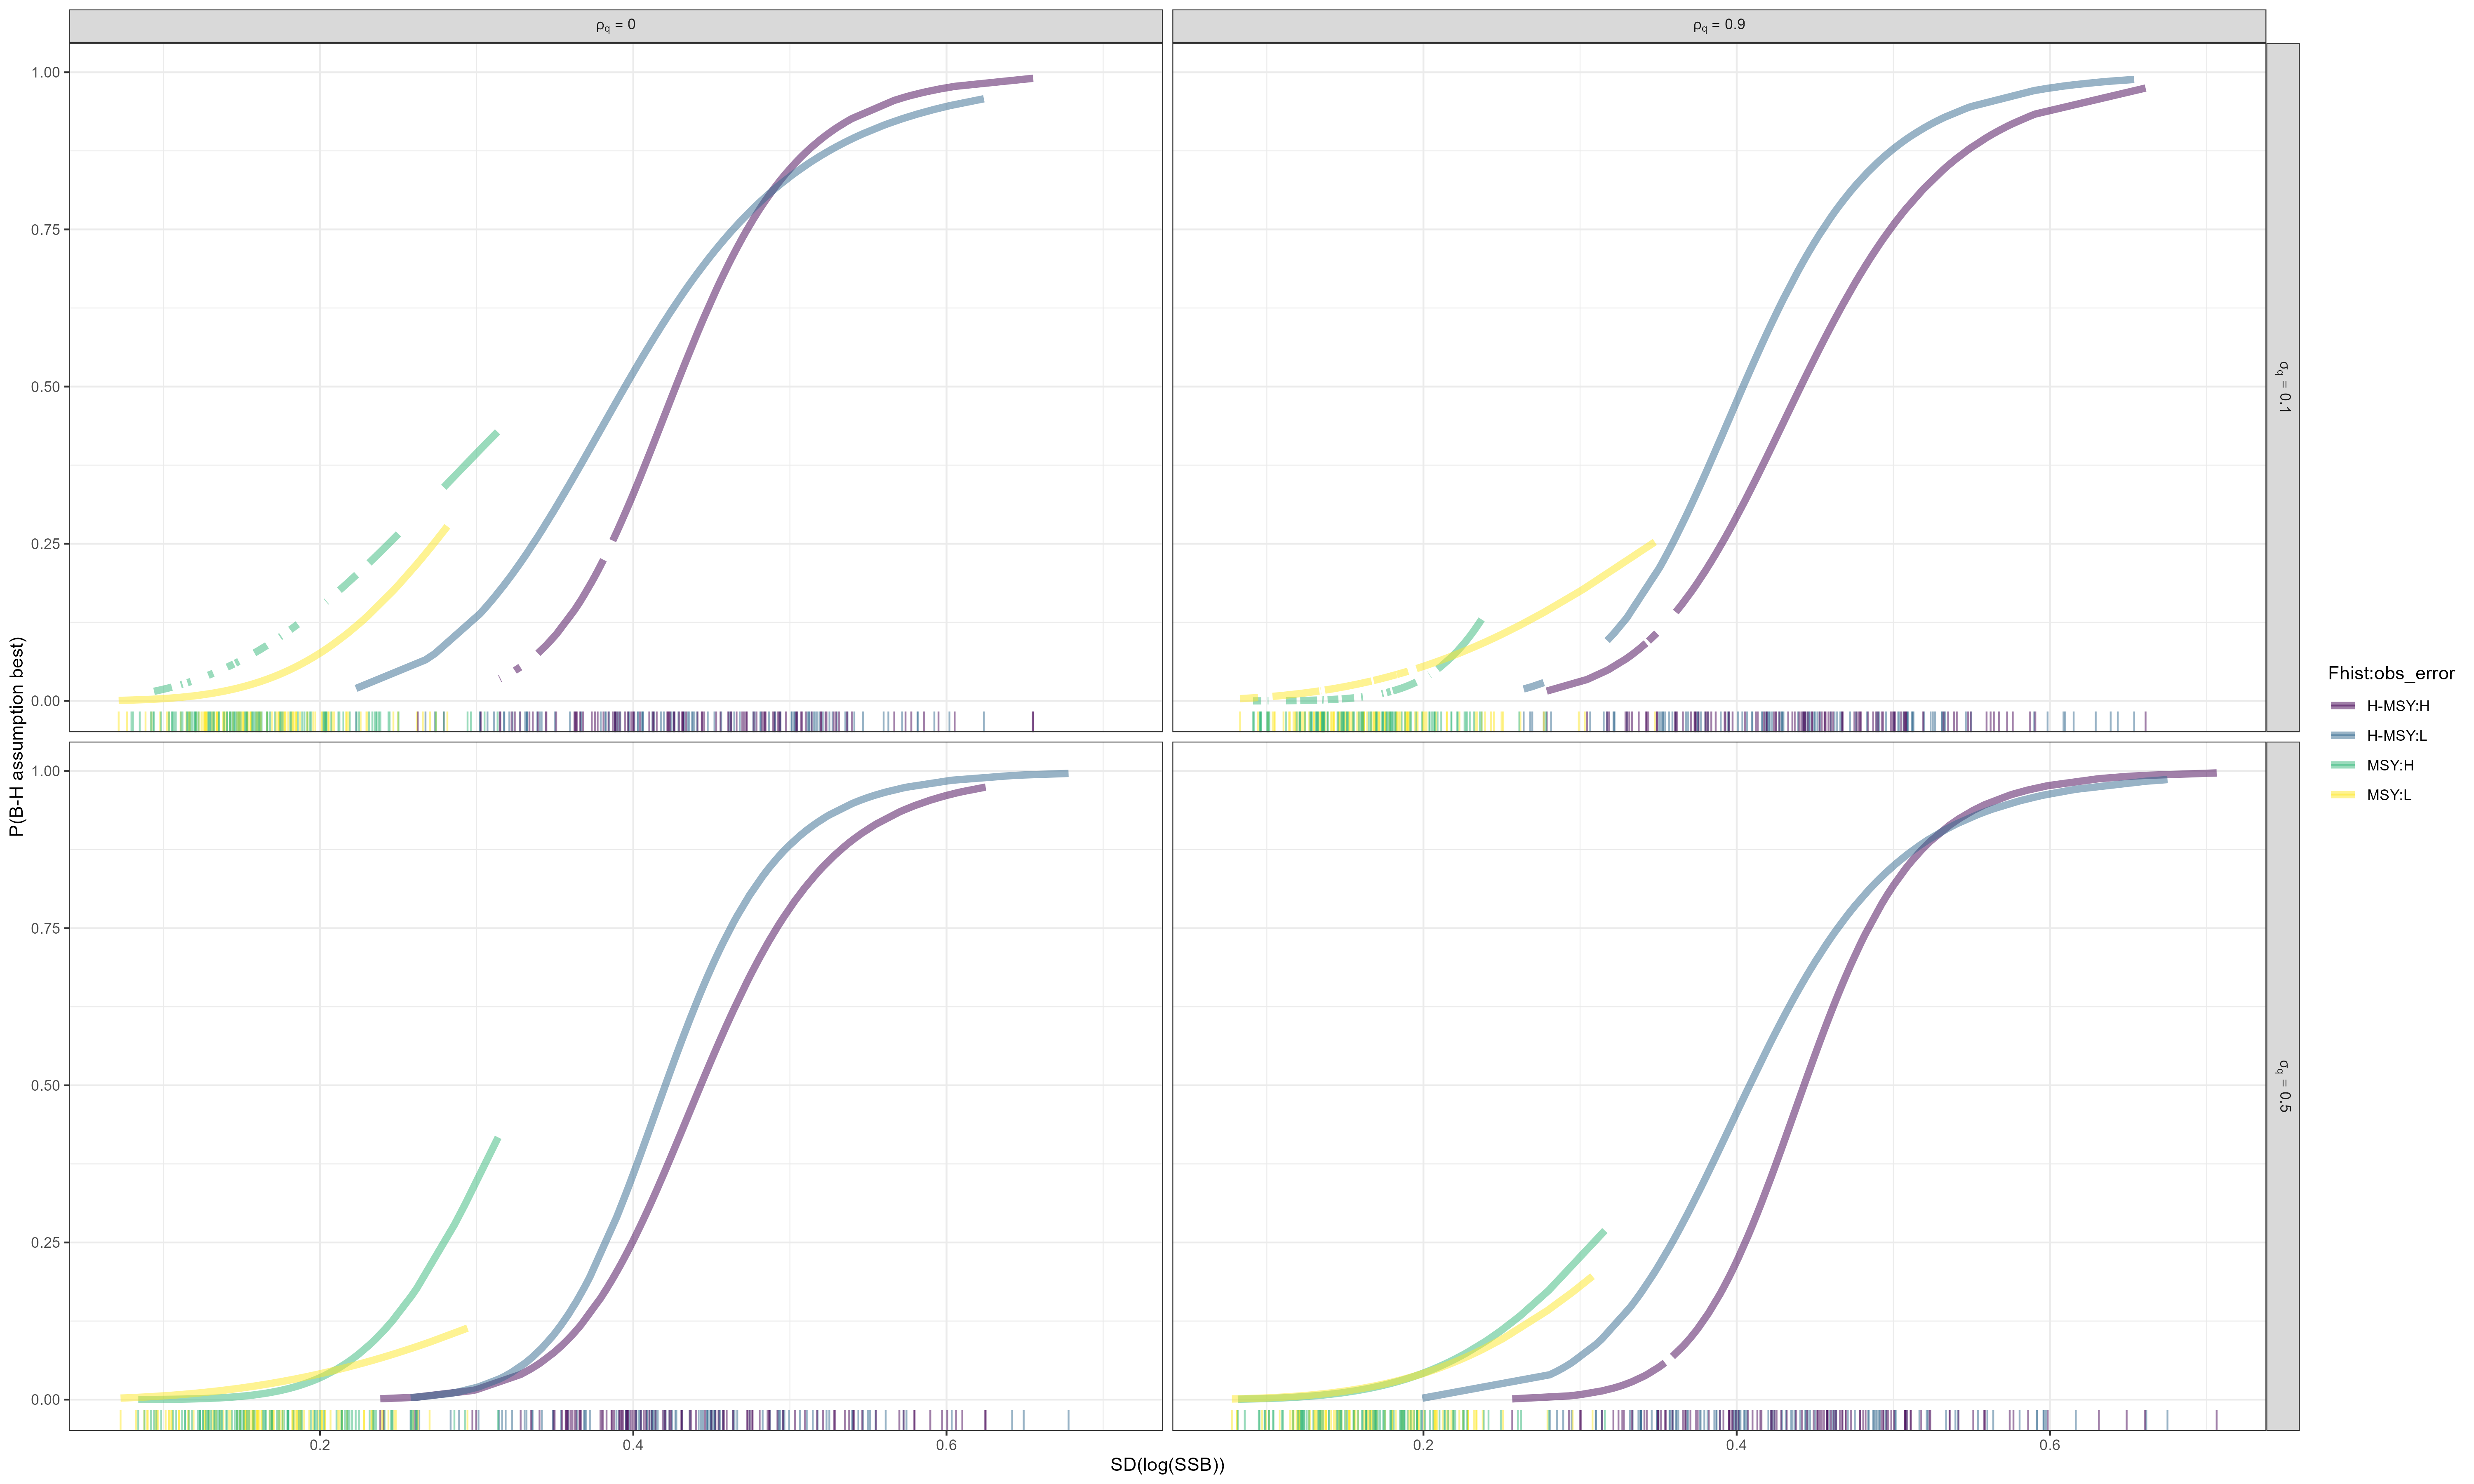
\includegraphics[width = \textwidth]{q_om_MF_pred_BH_best.png}
\end{center}
\end{figure}

\begin{figure}
\caption{Predicted probability of AIC preferring BH model as a function of the variation of population SSB. Operating and estimating models have matching R+q process error structures. Estimating models allow estimation of mean M.}\label{q_om_ME_BH_glm_AIC_plots}
\begin{center}
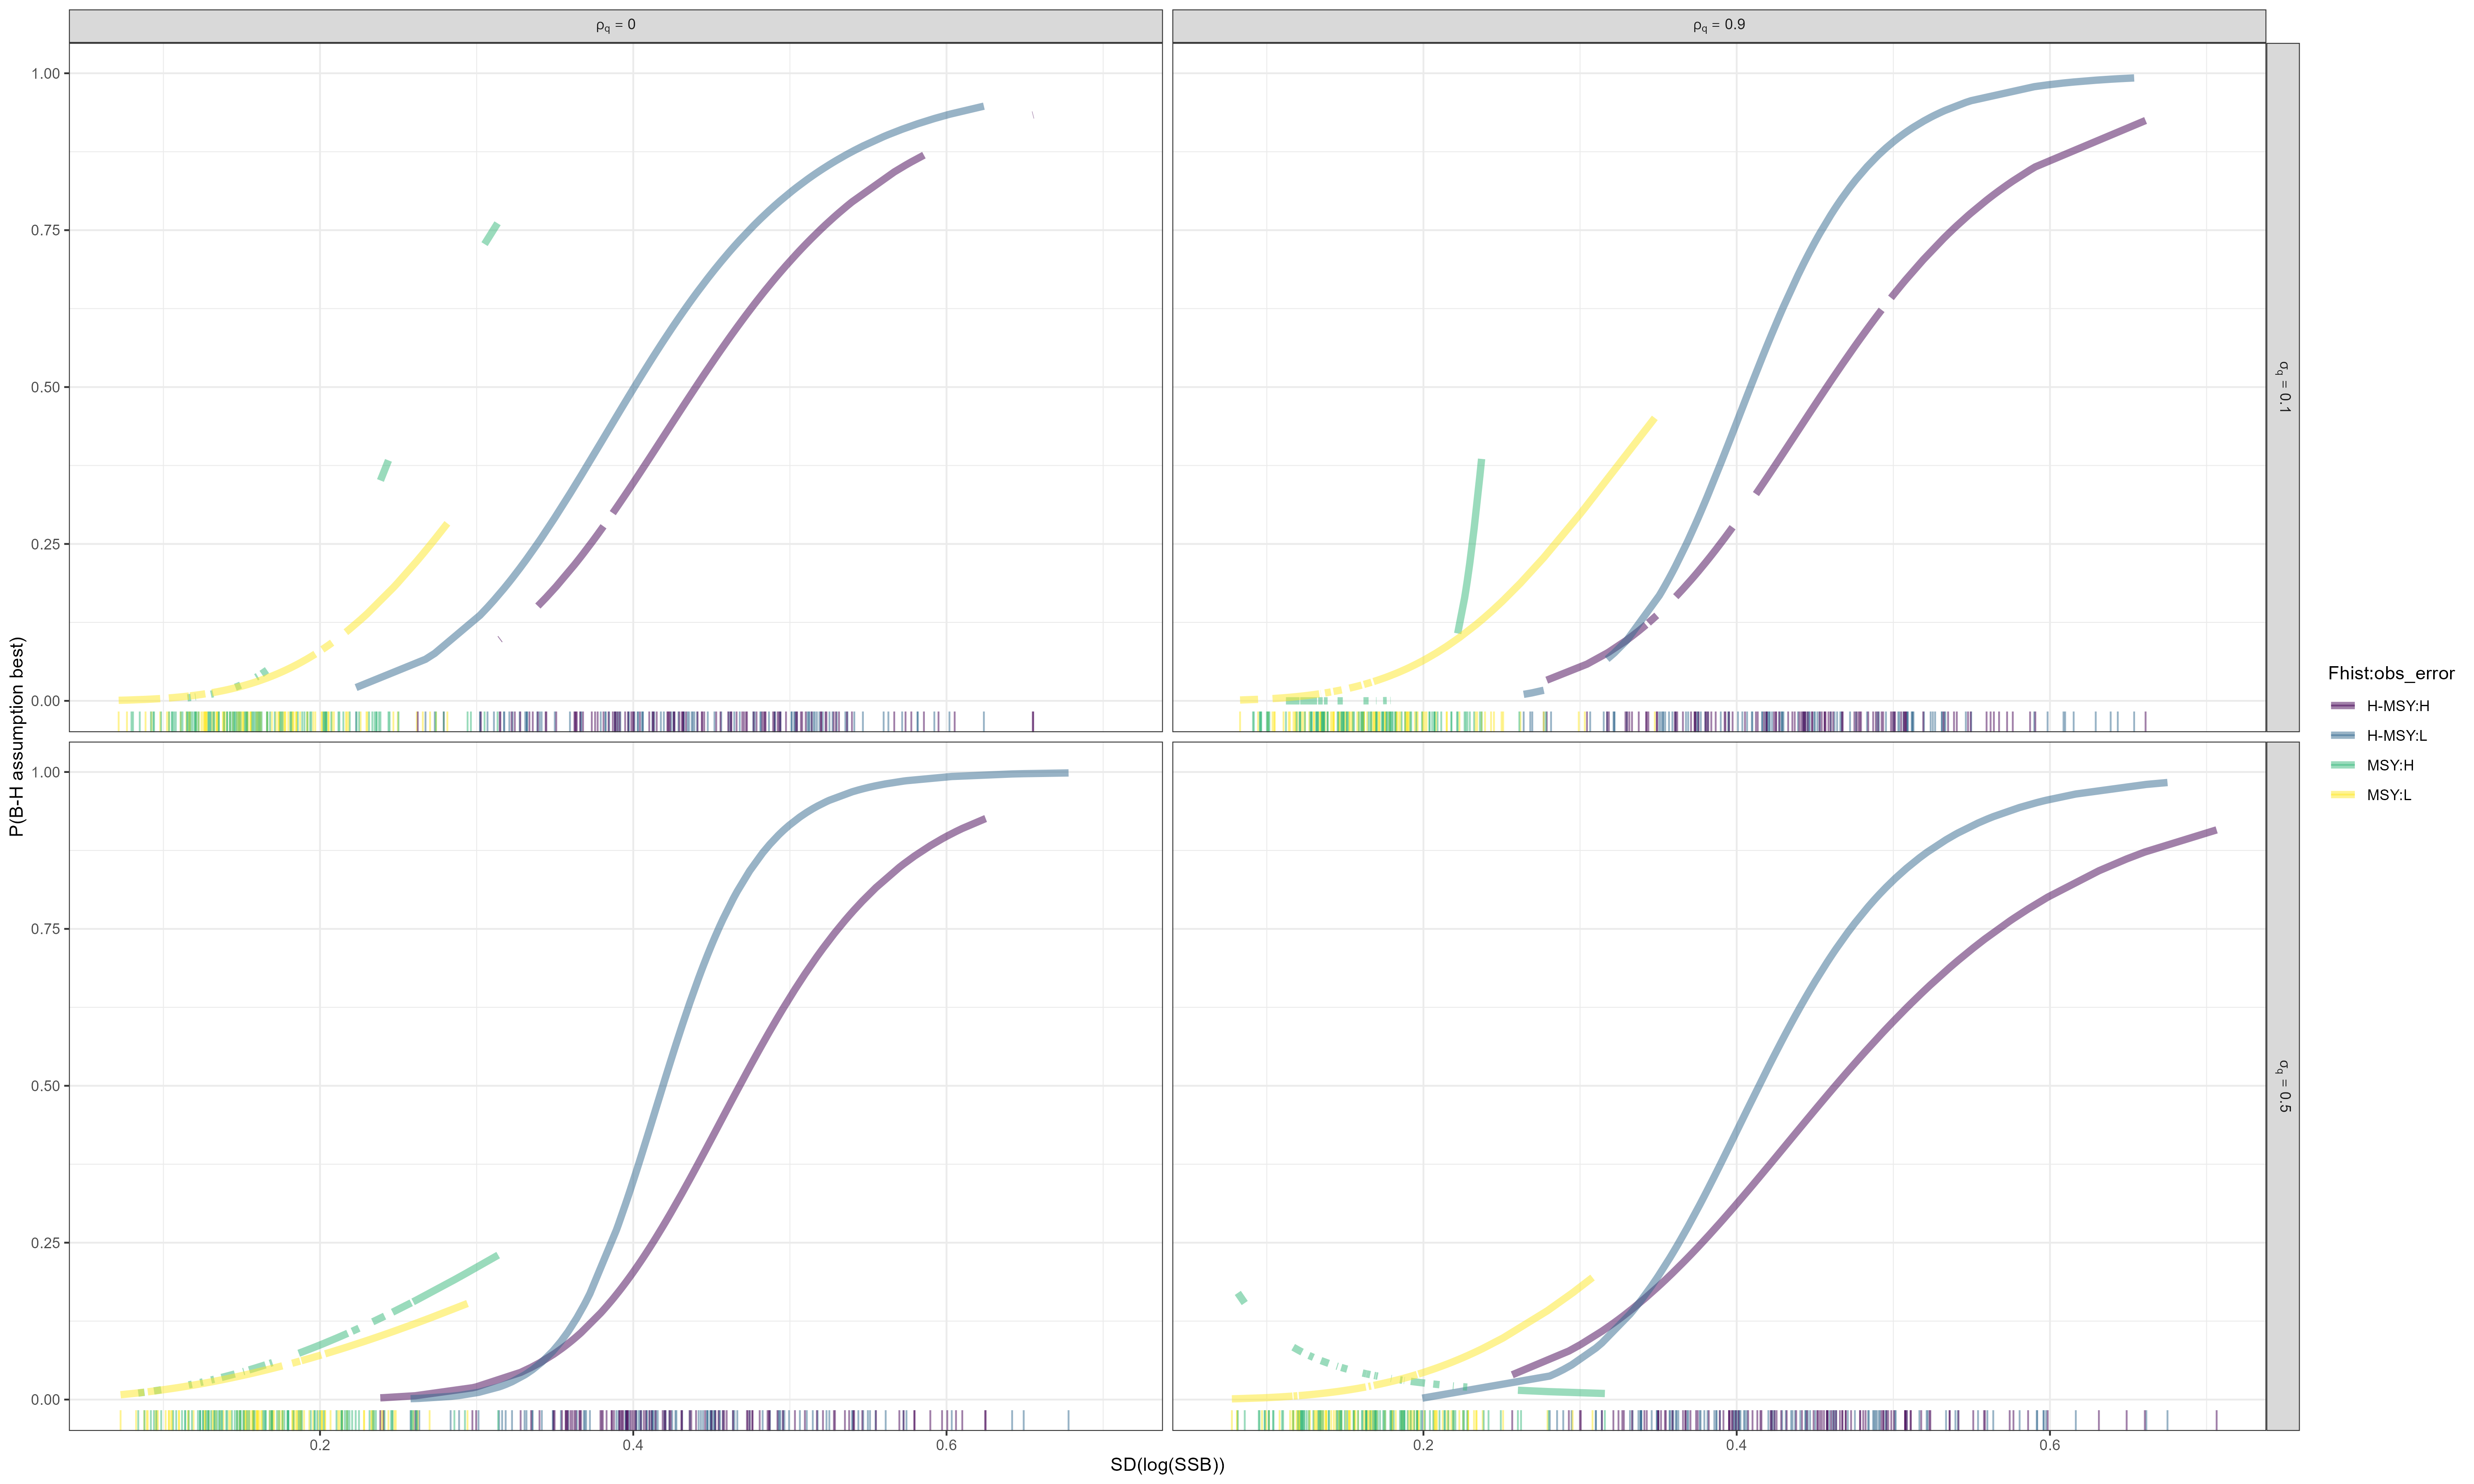
\includegraphics[width = \textwidth]{q_om_ME_pred_BH_best.png}
\end{center}
\end{figure}

\clearpage

\begin{landscape}
\begin{figure}
\caption{Median relative bias of SSB for estimating models fitted to data sets simulated with R and R+S process errors.  Estimation models do not assume a stock-recruit function and M is fixed at the true value.}\label{naa_om_em_R_MF_relbias_ssb}
\begin{center}
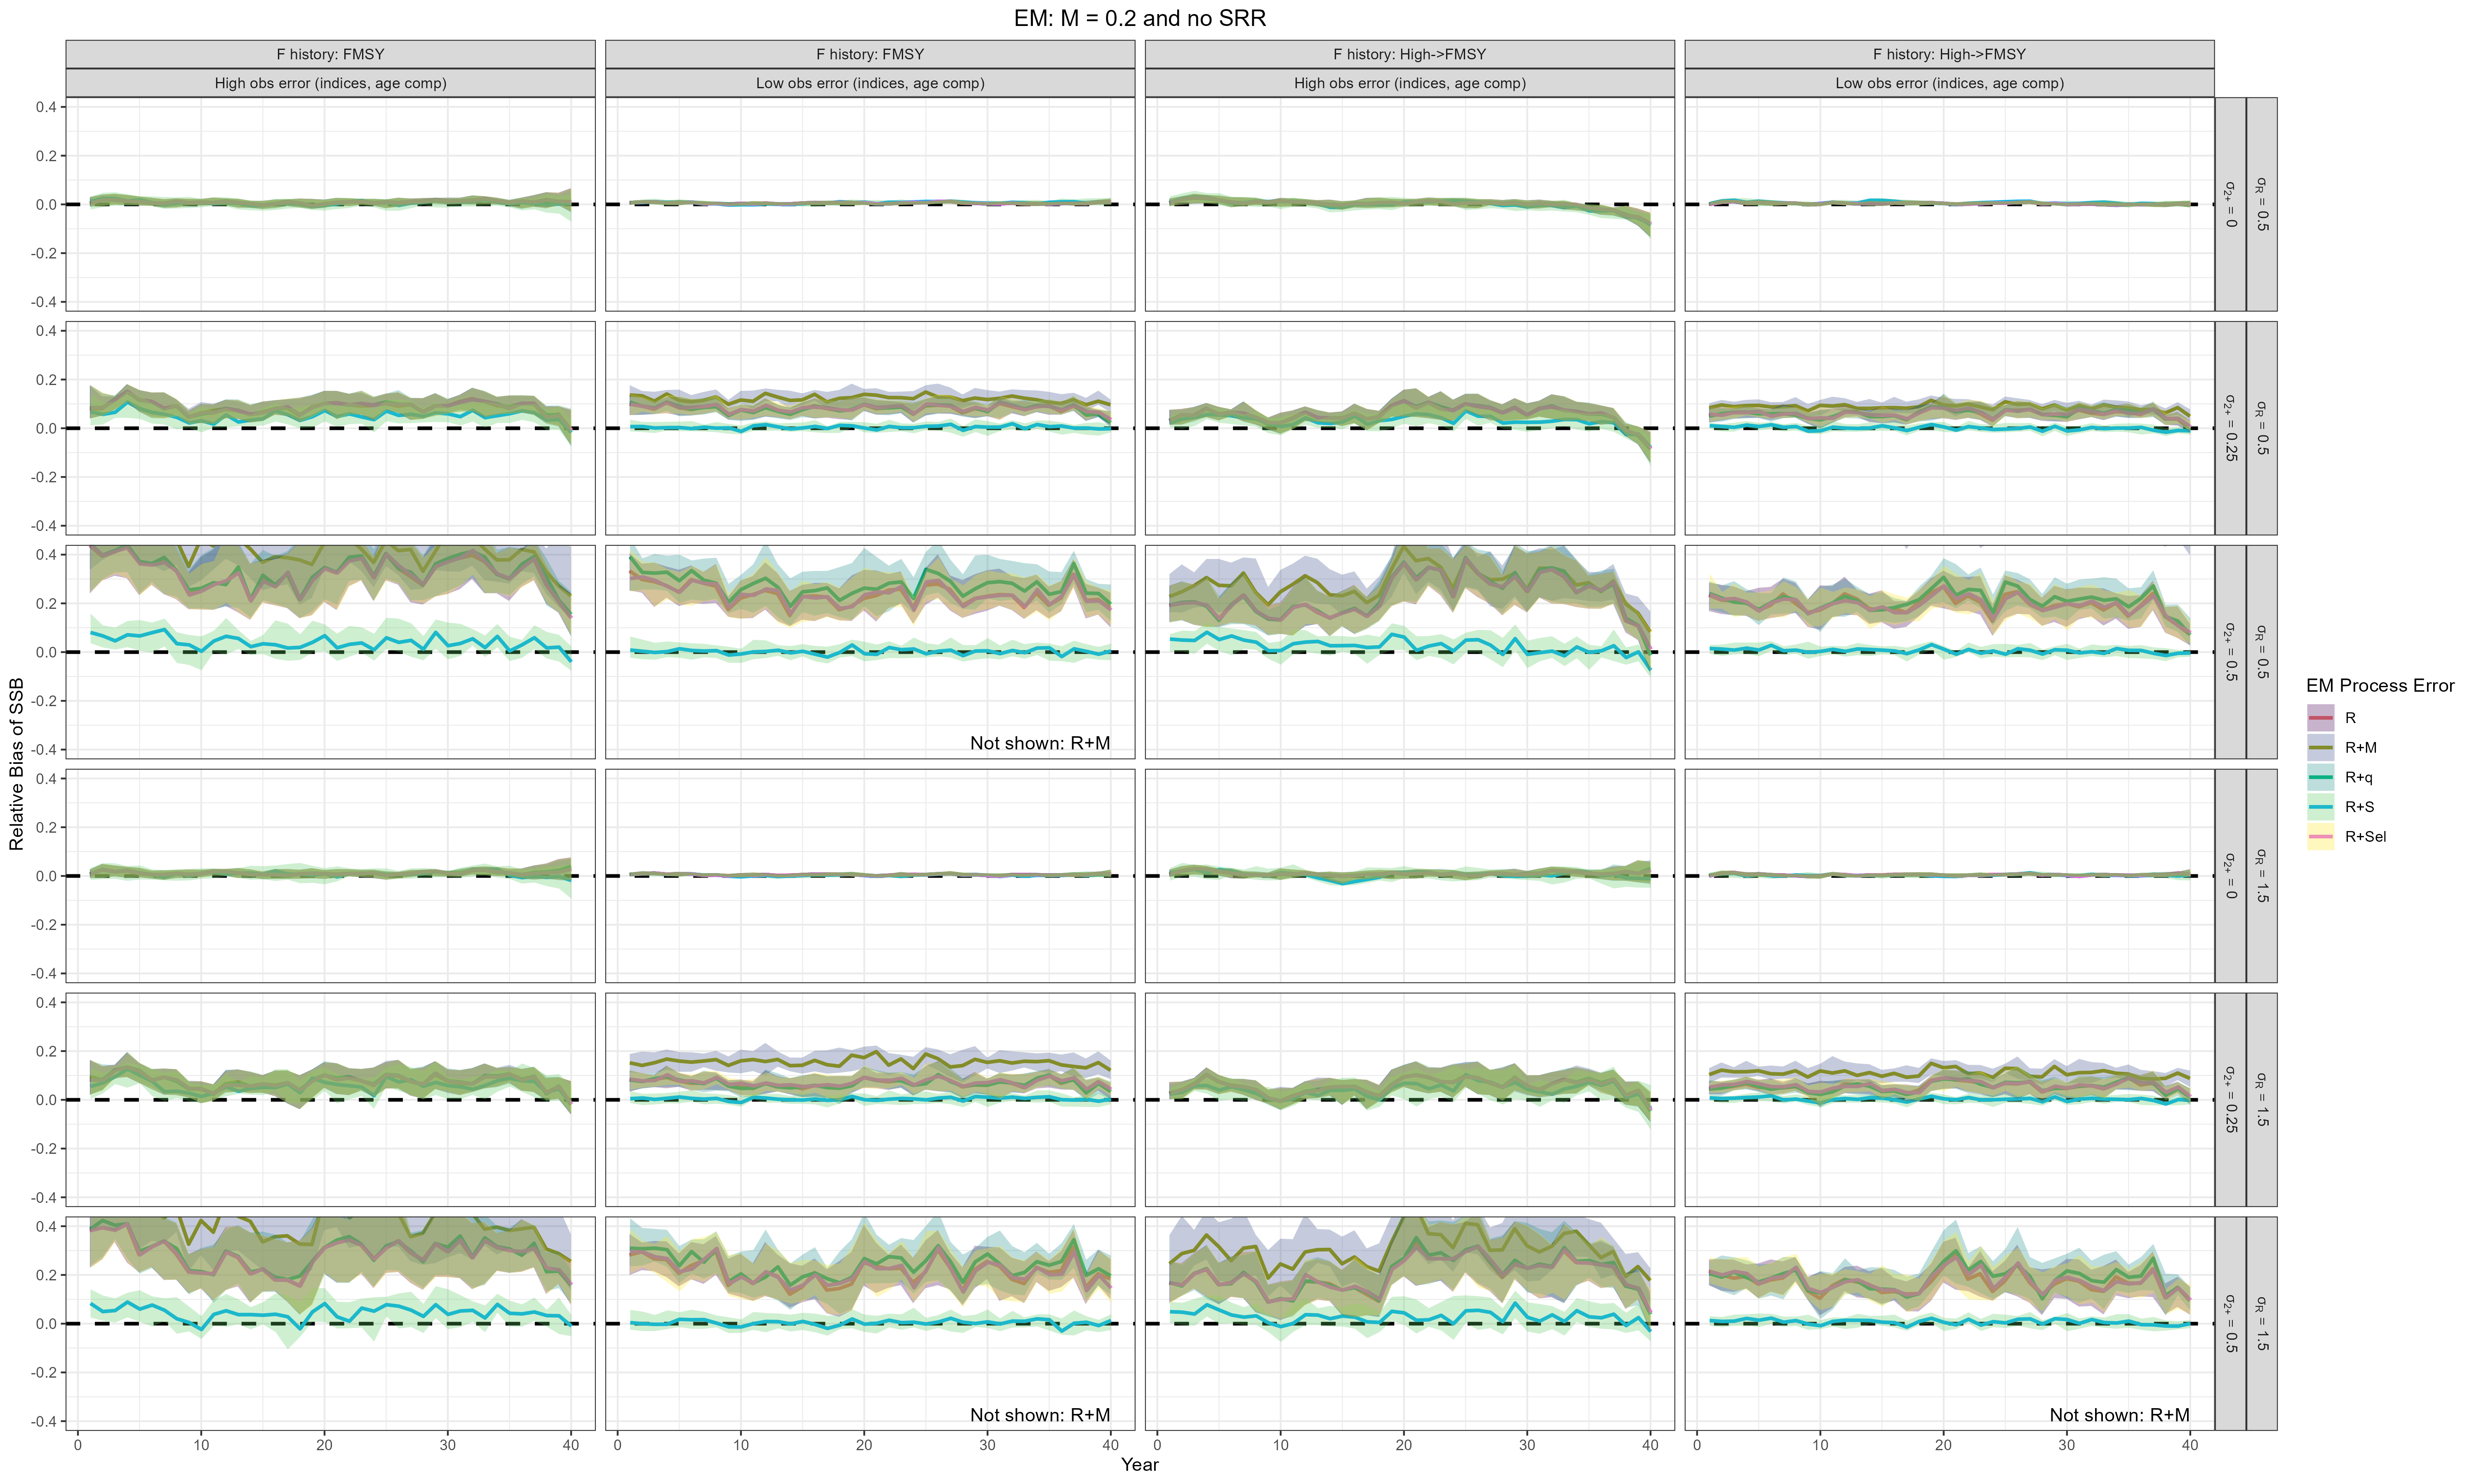
\includegraphics[width = \textwidth]{naa_om_R_MF_relbias_ssb.png}
\end{center}
\end{figure}
\end{landscape}

\begin{landscape}
\begin{figure}
\caption{Median relative bias of SSB for estimating models fitted to data sets simulated with R and R+S process errors. Estimation models do not assume a stock-recruit relationship and estimate M.}\label{naa_om_em_R_ME_relbias_ssb}
\begin{center}
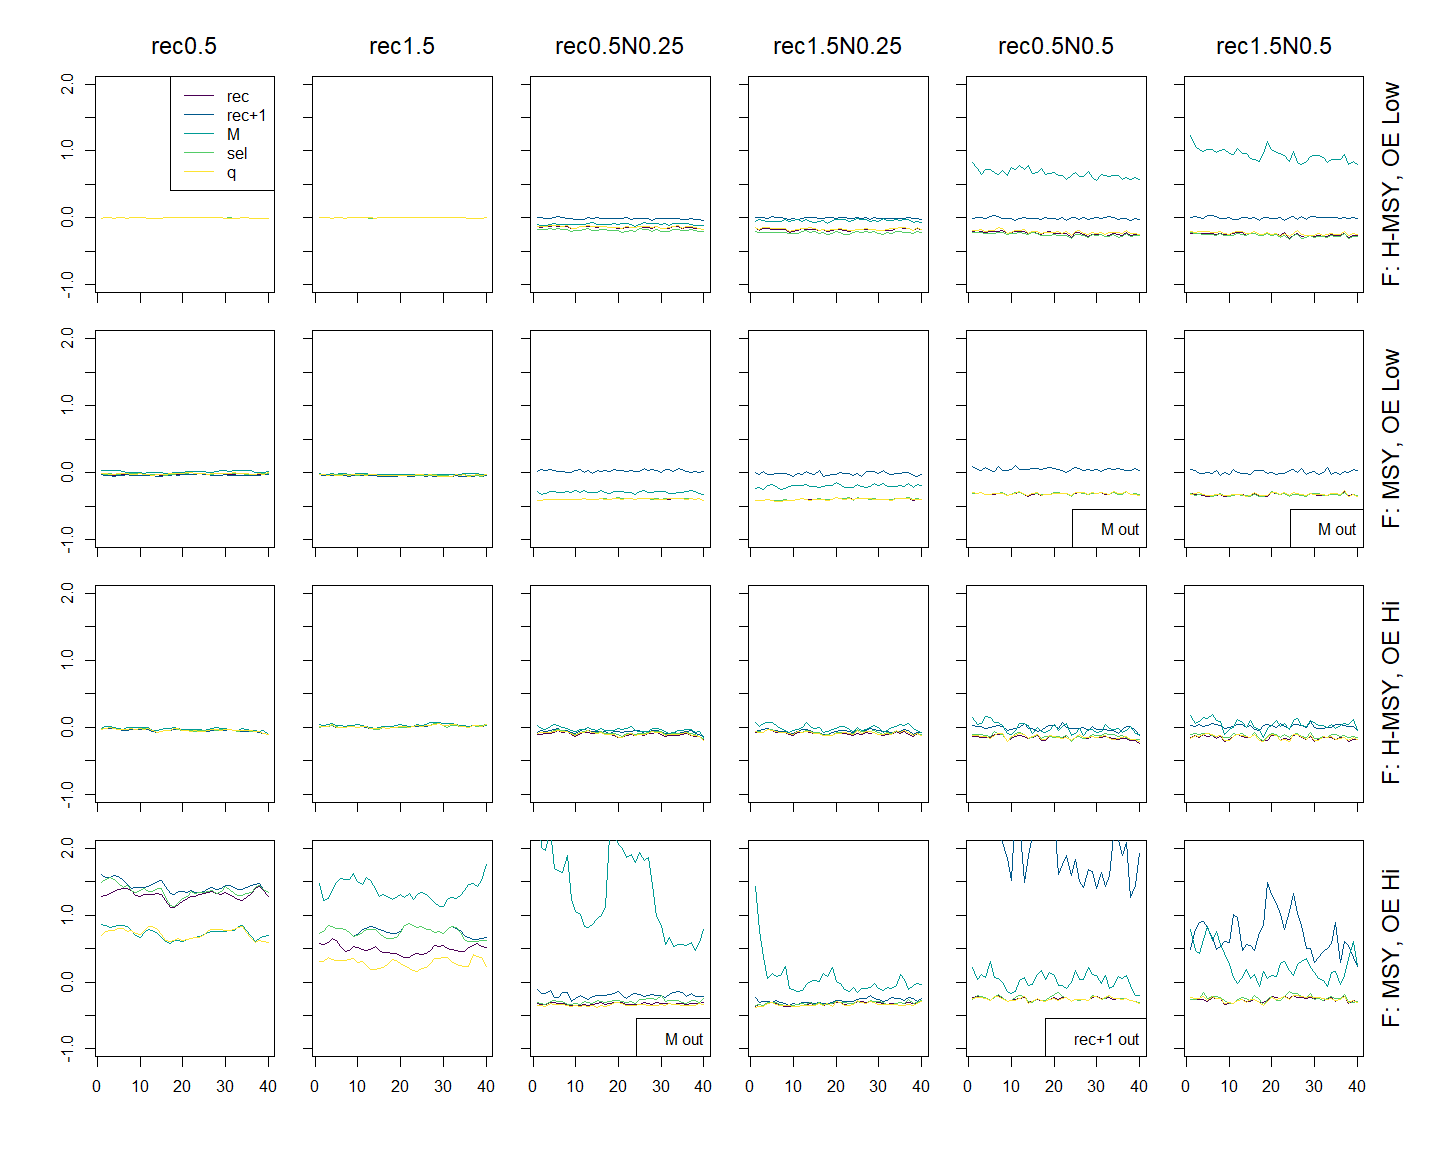
\includegraphics[width = \textwidth]{naa_om_R_ME_relbias_ssb.png}
\end{center}
\end{figure}
\end{landscape}

\begin{landscape}
\begin{figure}
\caption{Median relative bias of SSB for estimating models fitted to data sets simulated with R and R+S process errors. Estimation models assume a BH stock-recruitment function and M is fixed at the true value.}\label{naa_om_em_BH_MF_relbias_ssb}
\begin{center}
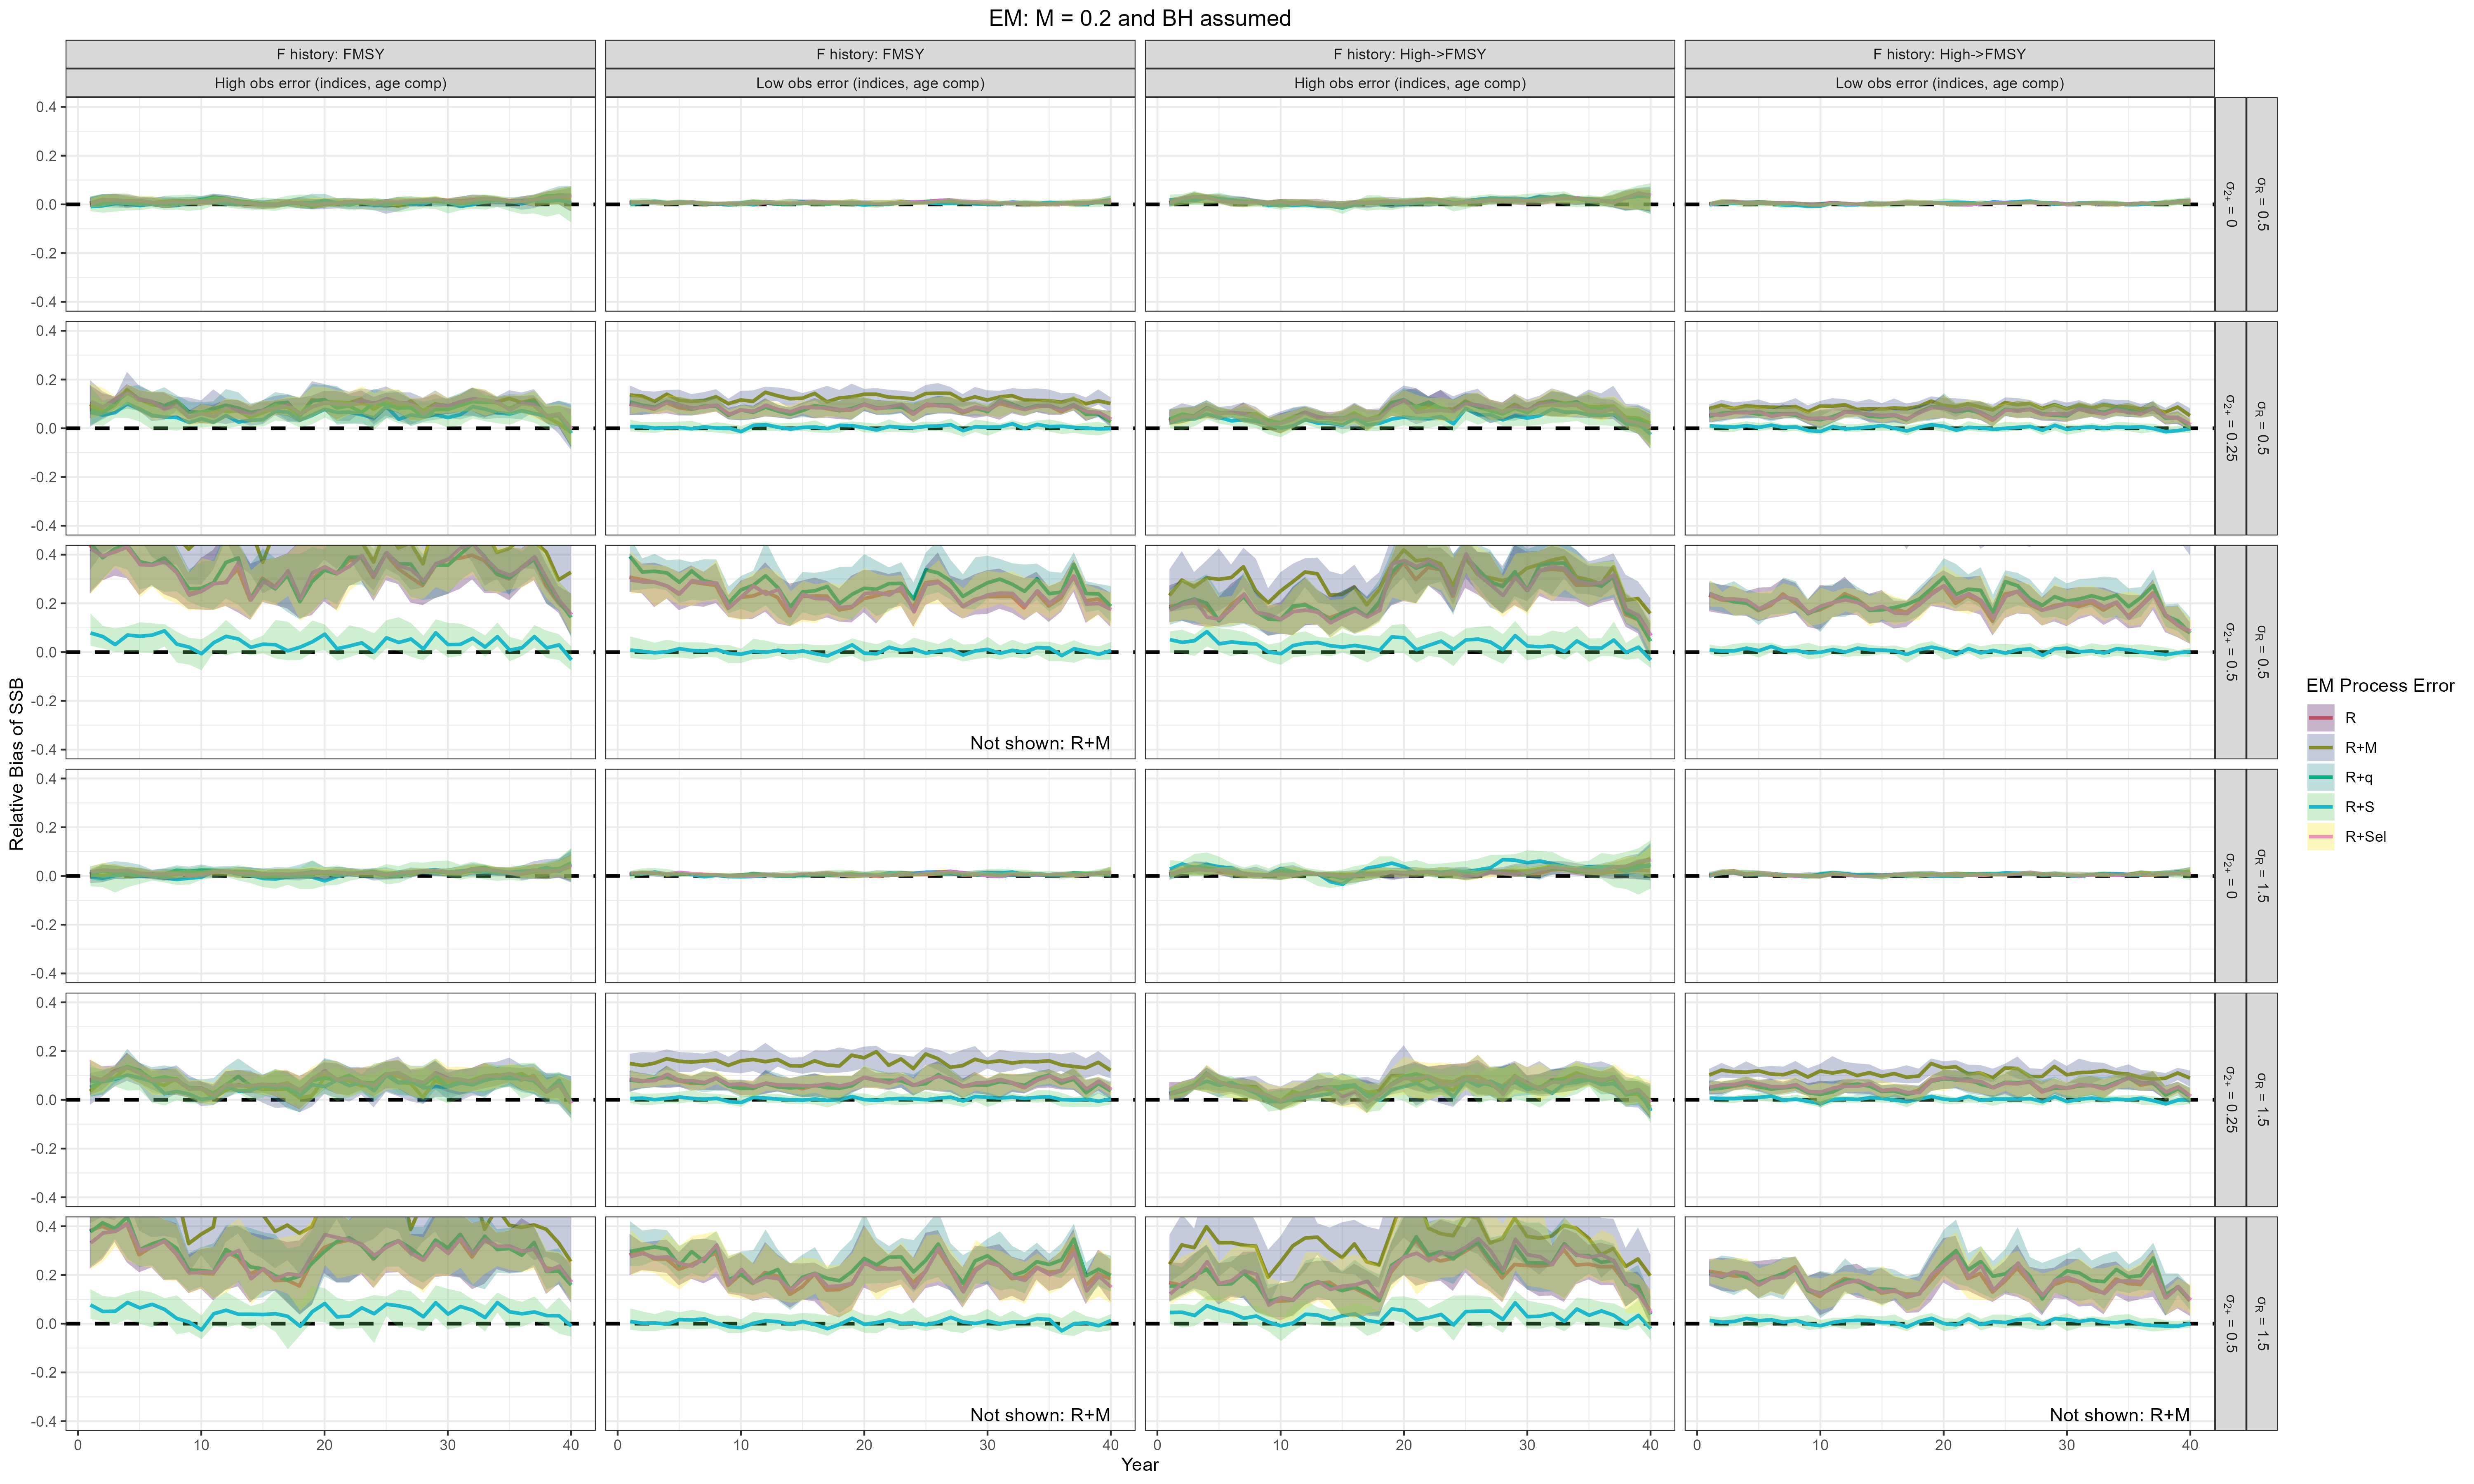
\includegraphics[width = \textwidth]{naa_om_BH_MF_relbias_ssb.png}
\end{center}
\end{figure}
\end{landscape}

\begin{landscape}
\begin{figure}
\caption{Median relative bias of SSB for estimating models fitted to data sets simulated with R and R+S process errors. Estimation models assume a BH stock-recruitment function and estimate M.}\label{naa_om_em_BH_ME_relbias_ssb}
\begin{center}
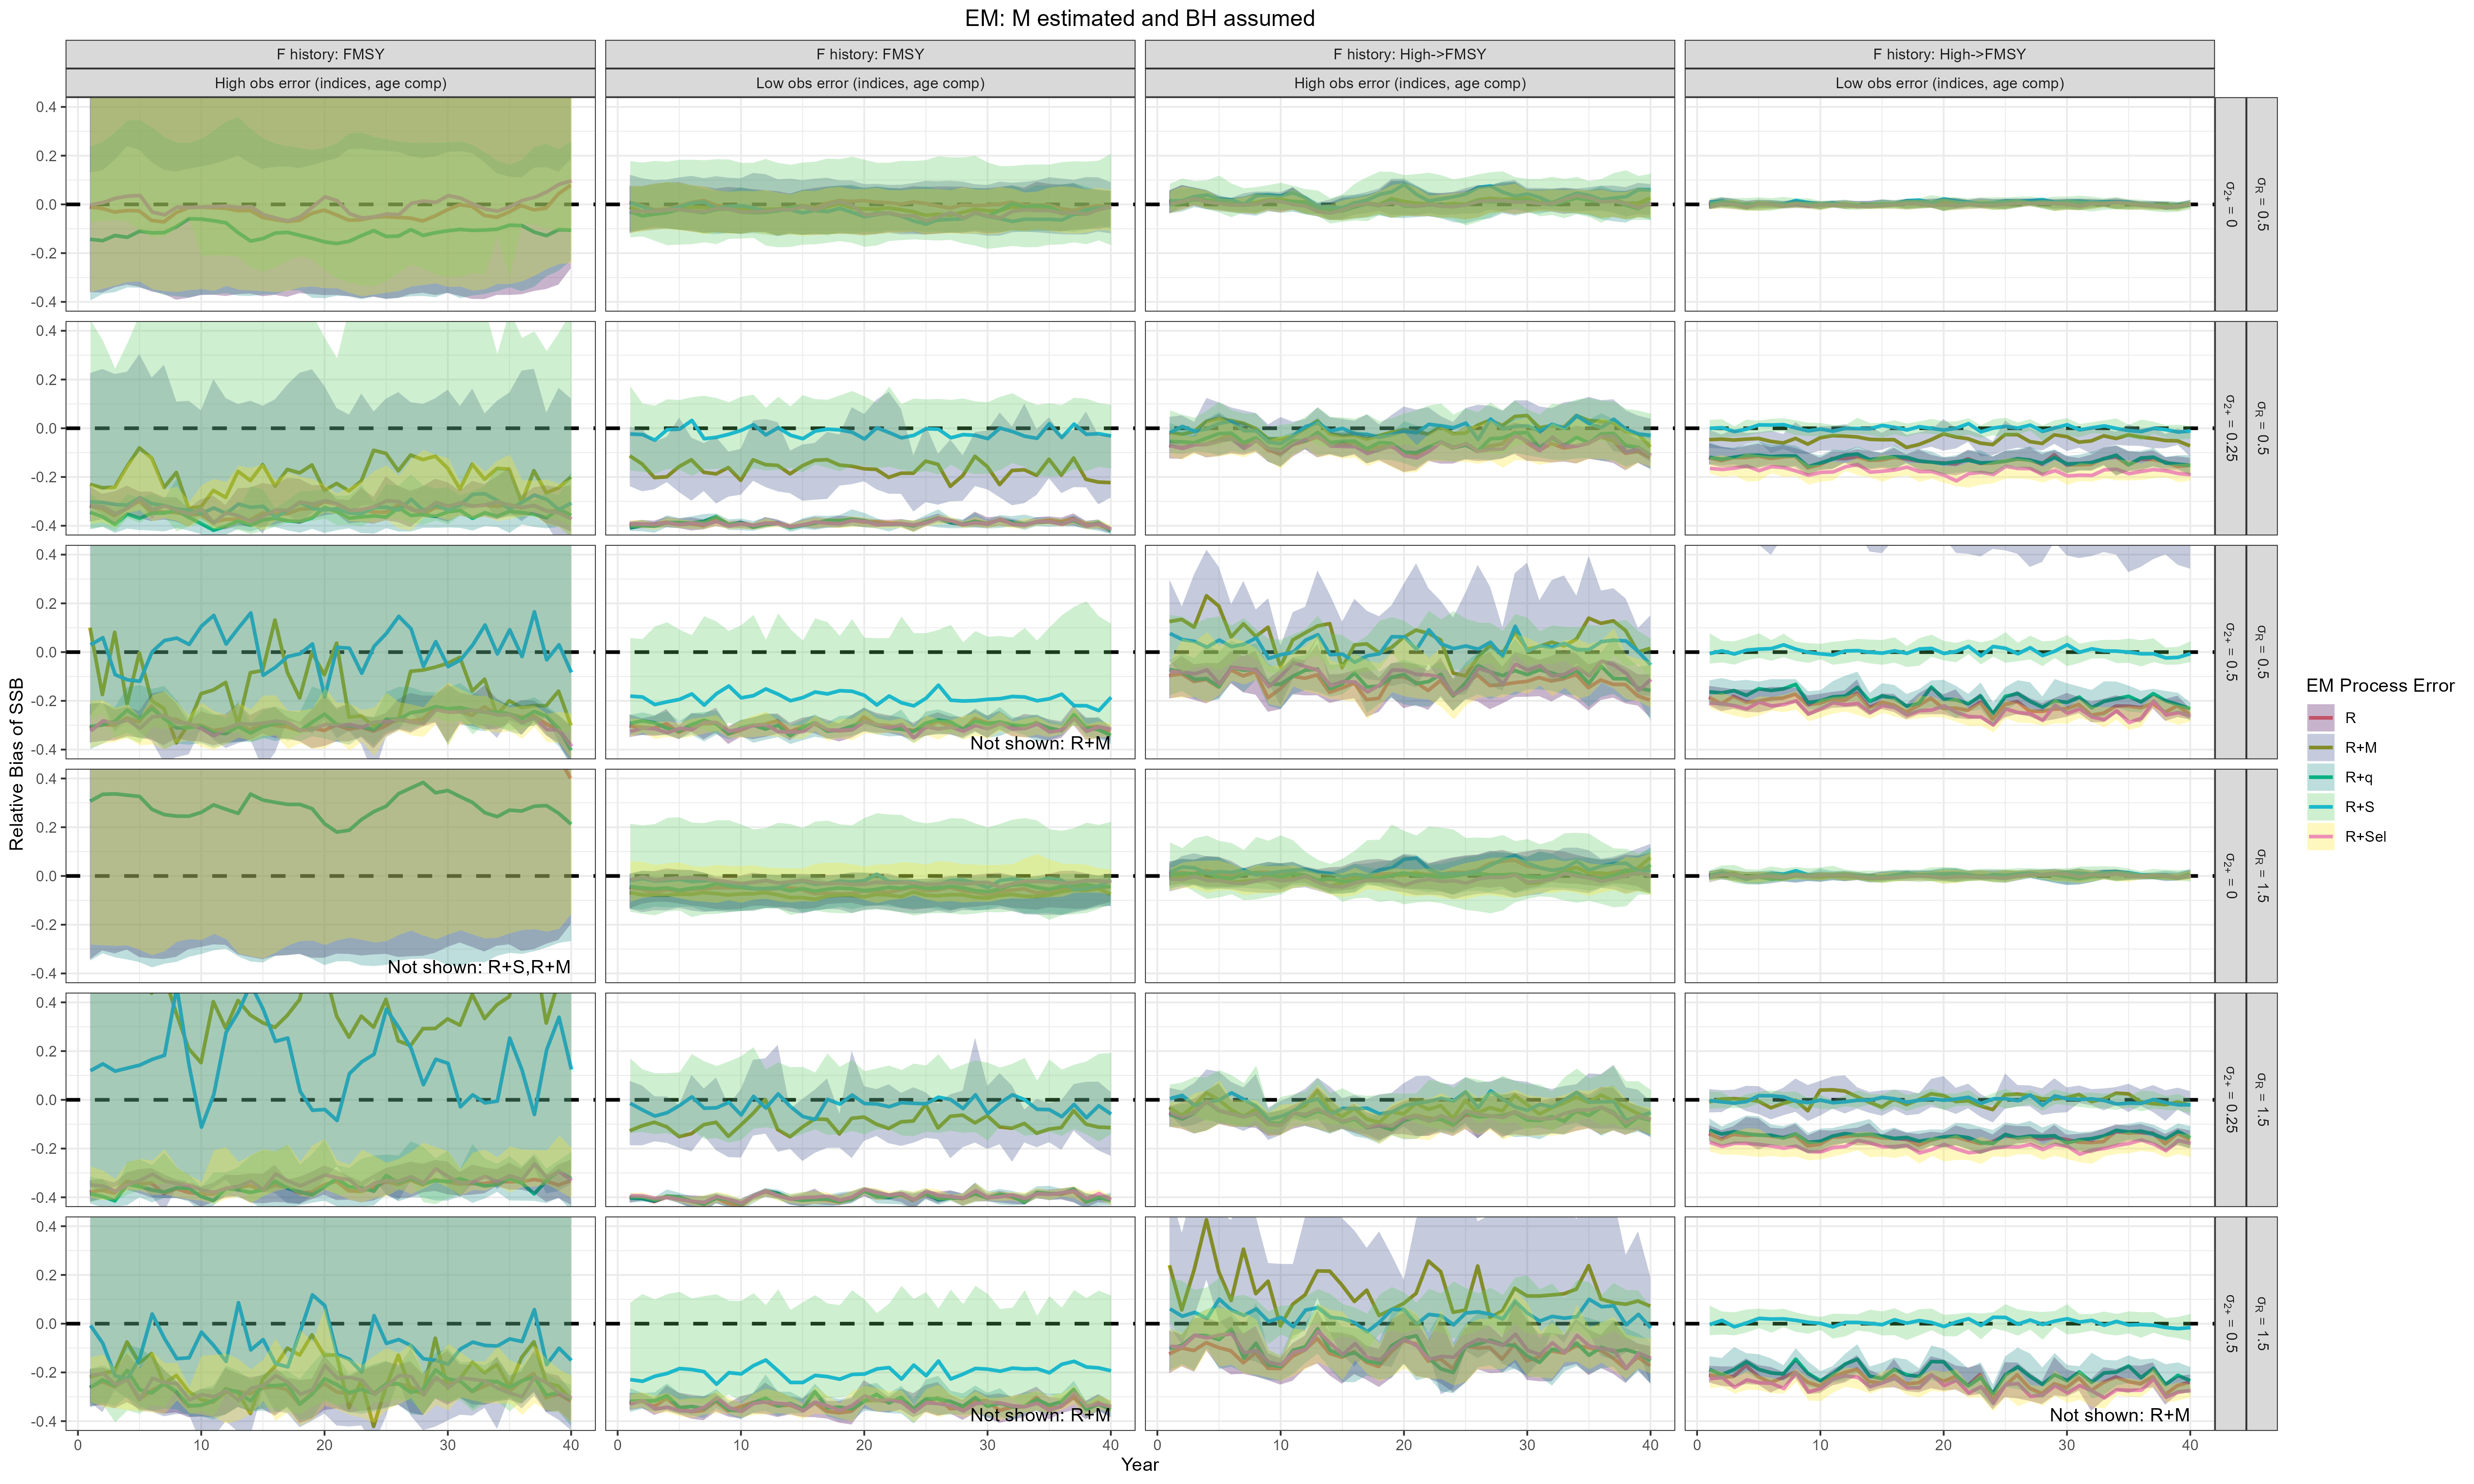
\includegraphics[width = \textwidth]{naa_om_BH_ME_relbias_ssb.png}
\end{center}
\end{figure}
\end{landscape}

\begin{landscape}
\begin{figure}
\caption{Median relative bias of SSB for estimating models fitted to data sets simulated with R+M process errors.  Estimation models do not assume a stock-recruit function and M is fixed at the true value.}\label{M_om_em_R_MF_relbias_ssb}
\begin{center}
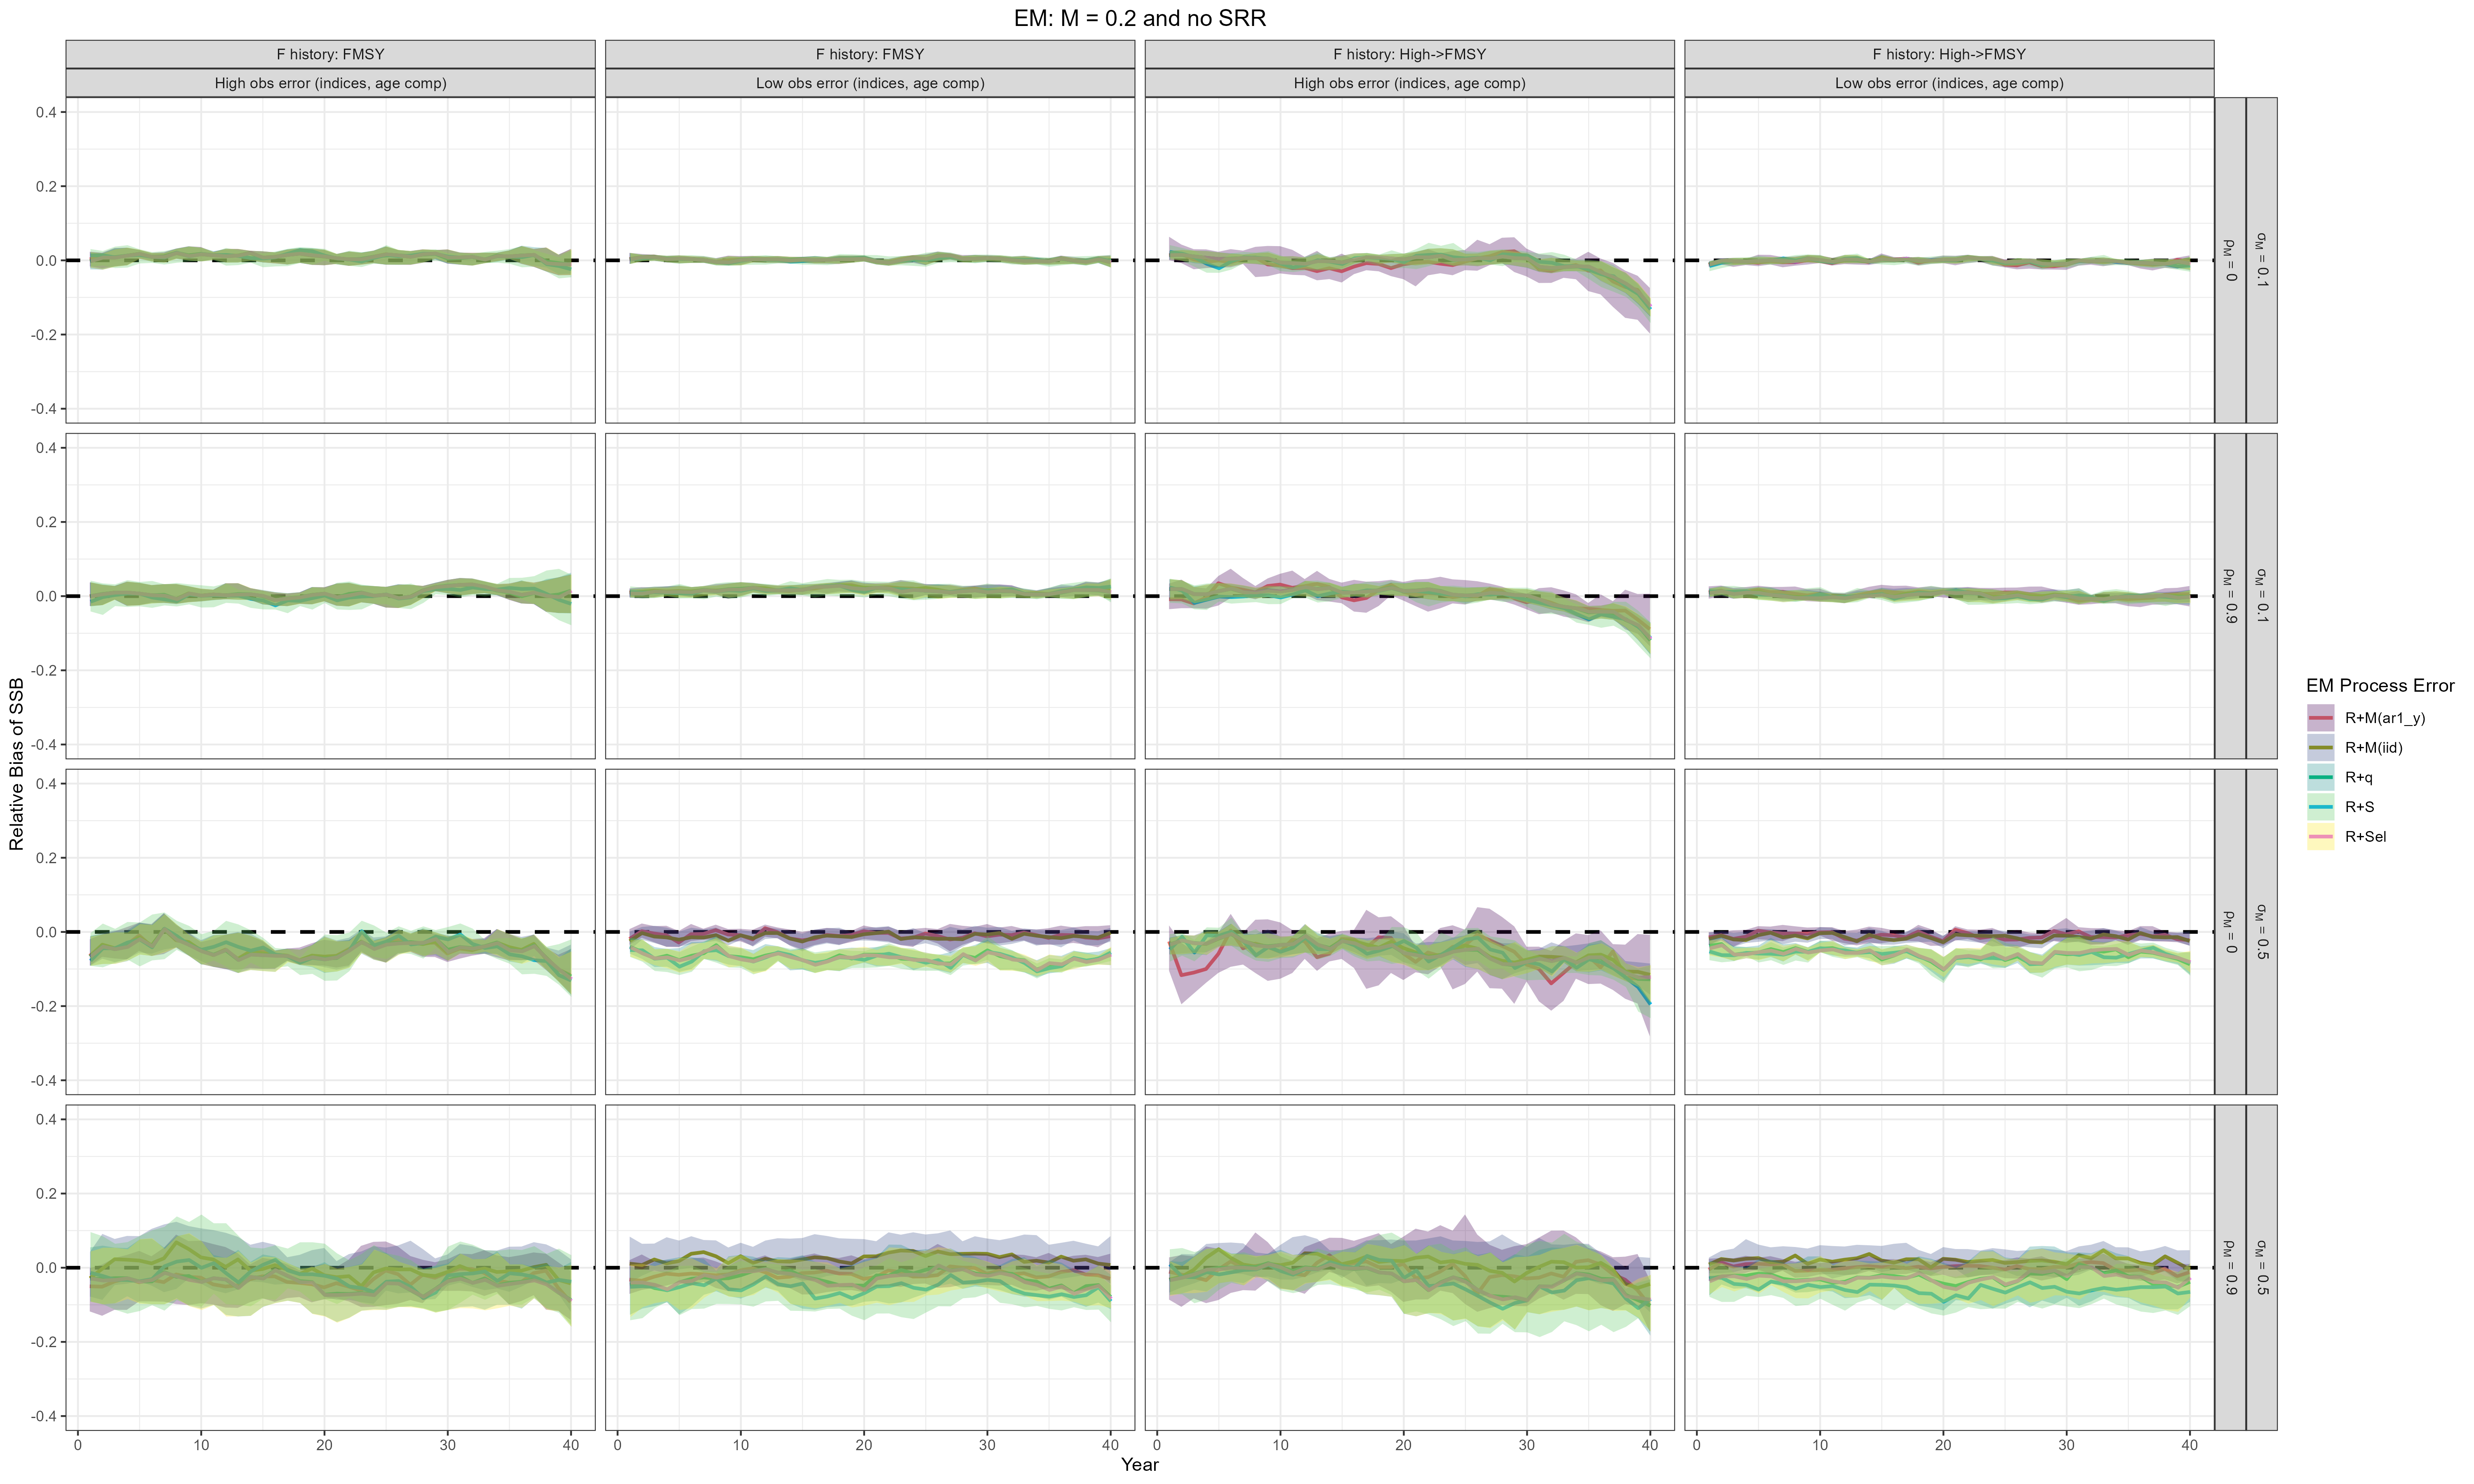
\includegraphics[width = \textwidth]{M_om_R_MF_relbias_ssb.png}
\end{center}
\end{figure}
\end{landscape}

\begin{landscape}
\begin{figure}
\caption{Median relative bias of SSB for estimating models fitted to data sets simulated with R+M process errors. Estimation models do not assume a stock-recruit relationship and estimate M.}\label{M_om_em_R_ME_relbias_ssb}
\begin{center}
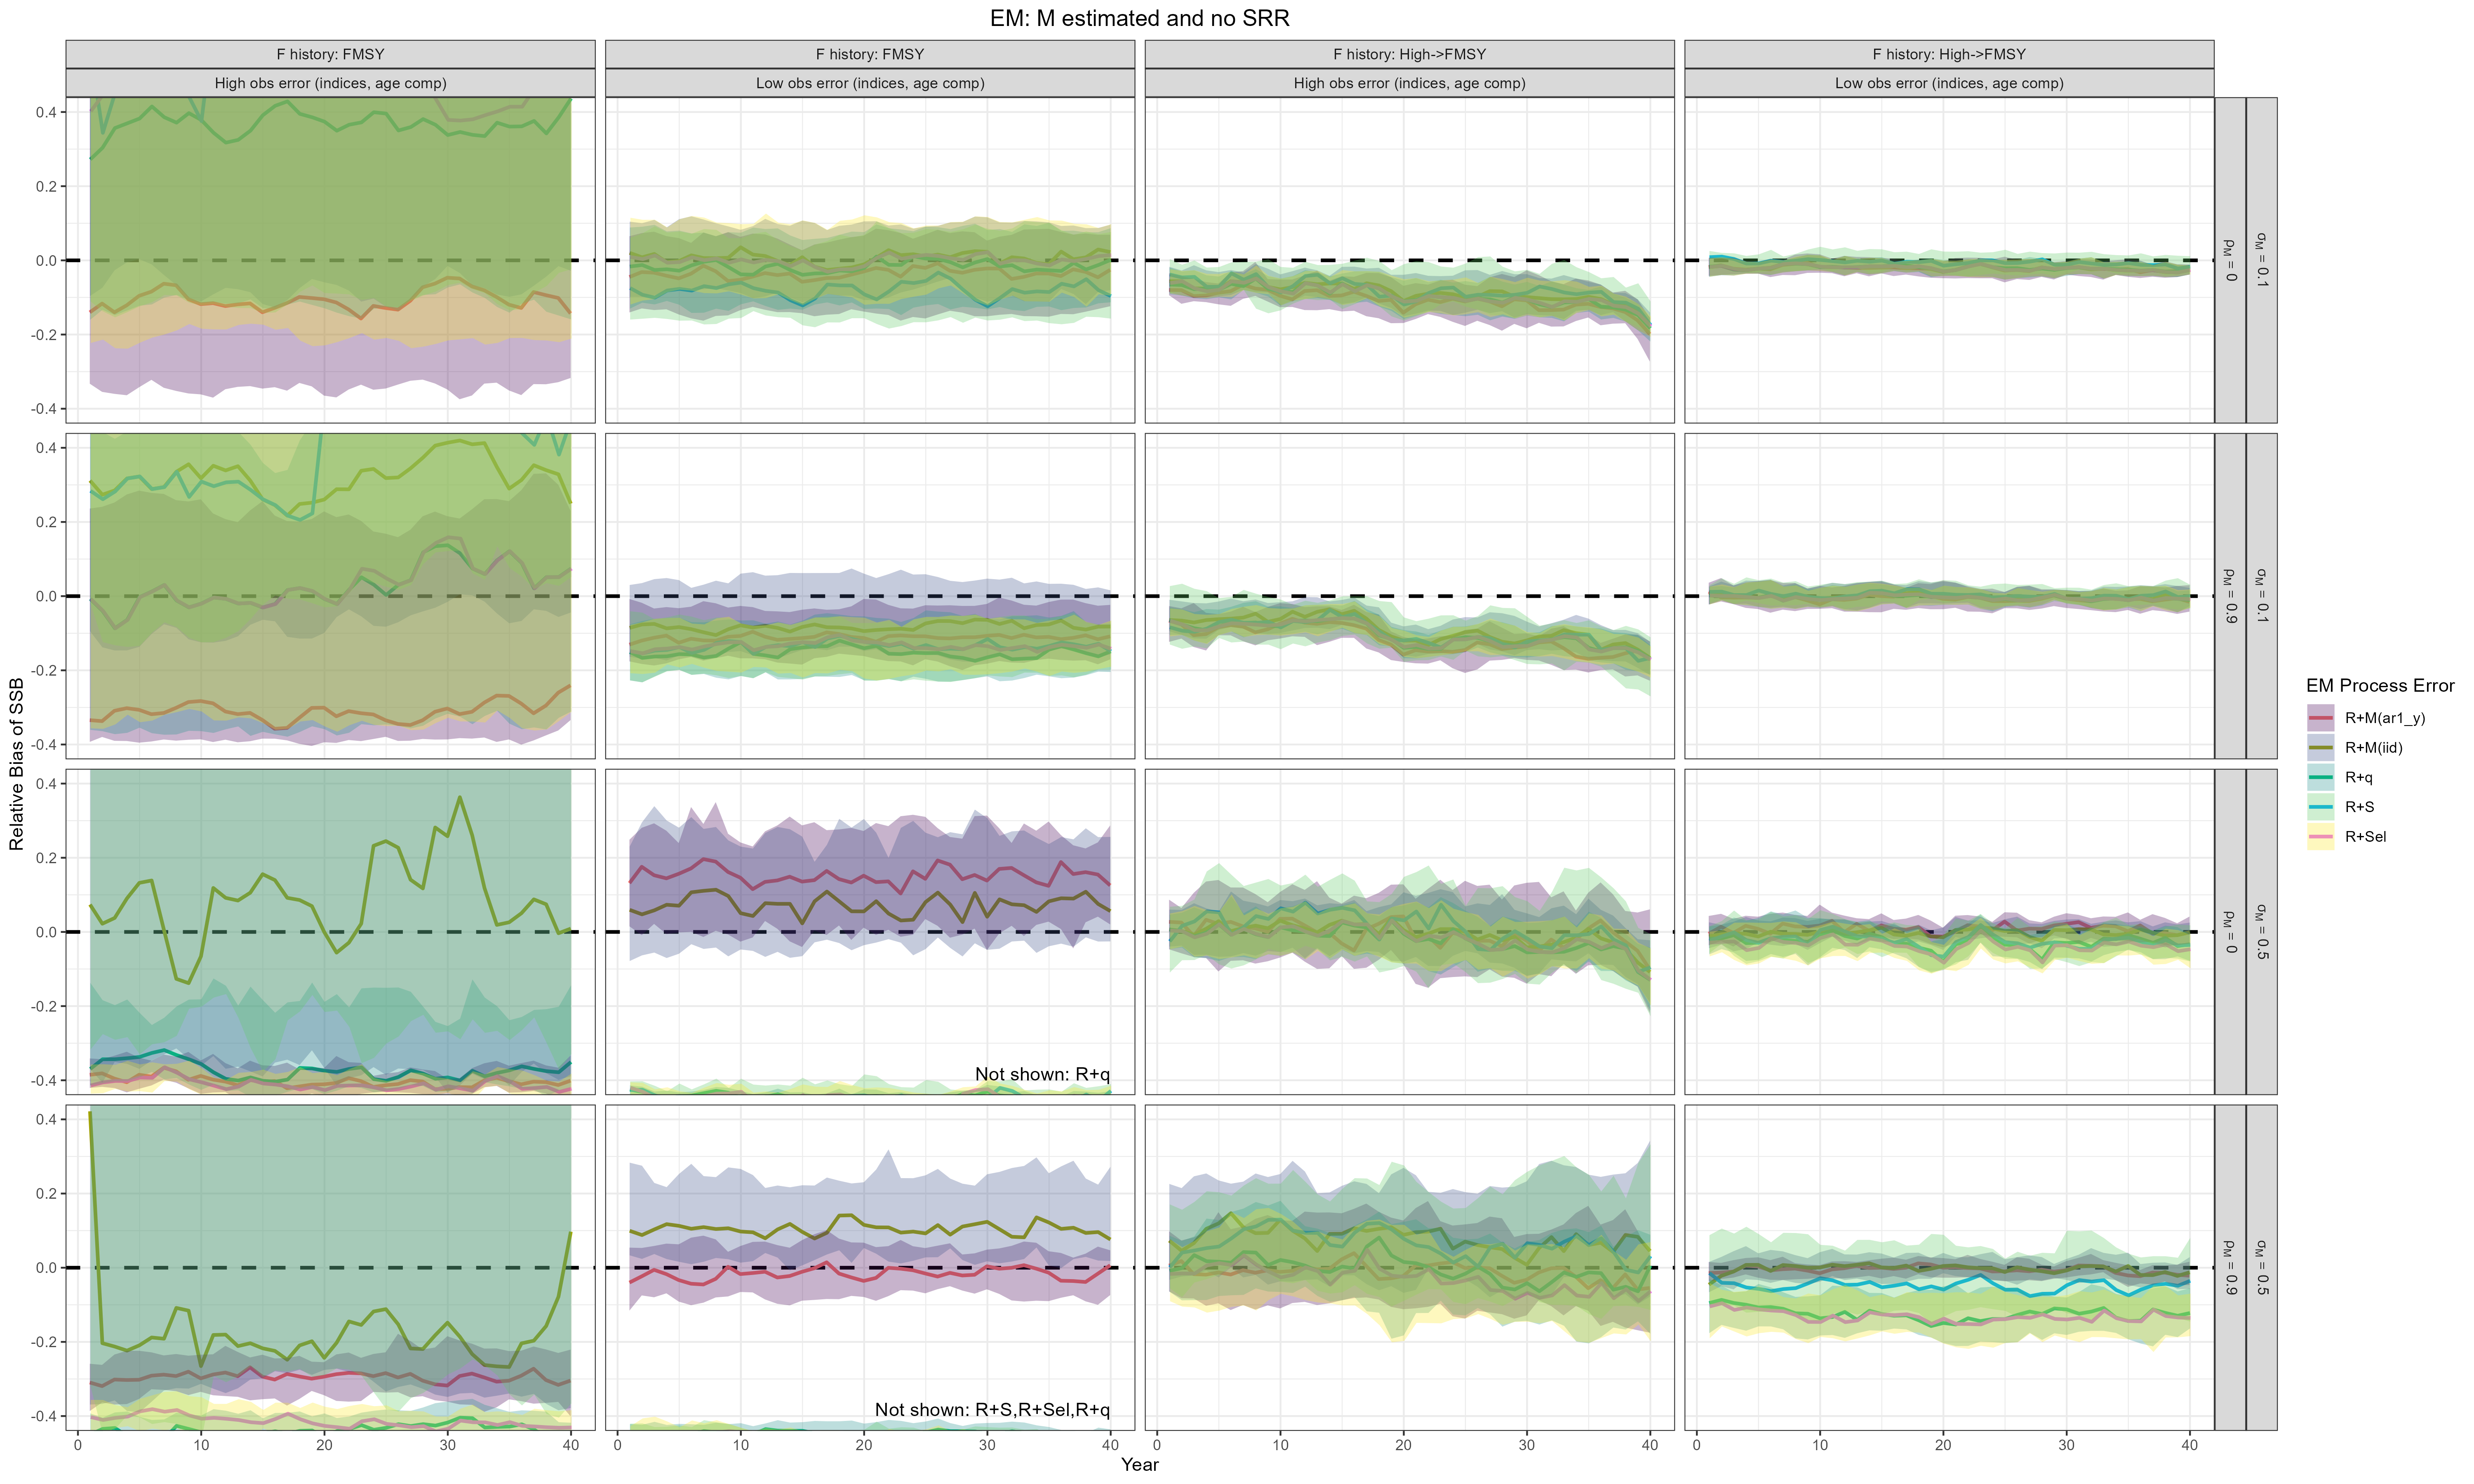
\includegraphics[width = \textwidth]{M_om_R_ME_relbias_ssb.png}
\end{center}
\end{figure}
\end{landscape}

\begin{landscape}
\begin{figure}
\caption{Median relative bias of SSB for estimating models fitted to data sets simulated with R+M process errors. Estimation models assume a BH stock-recruitment function and M is fixed at the true value.}\label{M_om_em_BH_MF_relbias_ssb}
\begin{center}
\includegraphics[width = \textwidth]{M_om_BH_MF_relbias_ssb.png}
\end{center}
\end{figure}
\end{landscape}

\begin{landscape}
\begin{figure}
\caption{Median relative bias of SSB for estimating models fitted to data sets simulated with R+M process errors. Estimation models assume a BH stock-recruitment function and estimate M.}\label{M_om_em_BH_ME_relbias_ssb}
\begin{center}
\includegraphics[width = \textwidth]{M_om_BH_ME_relbias_ssb.png}
\end{center}
\end{figure}
\end{landscape}

\begin{landscape}
\begin{figure}
\caption{Median relative bias of SSB for estimating models fitted to data sets simulated with R+Sel process errors.  Estimation models do not assume a stock-recruit function and M is fixed at the true value.}\label{Sel_om_em_R_MF_relbias_ssb}
\begin{center}
\includegraphics[width = \textwidth]{Sel_om_R_MF_relbias_ssb.png}
\end{center}
\end{figure}
\end{landscape}

\begin{landscape}
\begin{figure}
\caption{Median relative bias of SSB for estimating models fitted to data sets simulated with R+Sel process errors. Estimation models do not assume a stock-recruit relationship and estimate M.}\label{Sel_om_em_R_ME_relbias_ssb}
\begin{center}
\includegraphics[width = \textwidth]{Sel_om_R_ME_relbias_ssb.png}
\end{center}
\end{figure}
\end{landscape}

\begin{landscape}
\begin{figure}
\caption{Median relative bias of SSB for estimating models fitted to data sets simulated with R+Sel process errors. Estimation models assume a BH stock-recruitment function and M is fixed at the true value.}\label{Sel_om_em_BH_MF_relbias_ssb}
\begin{center}
\includegraphics[width = \textwidth]{Sel_om_BH_MF_relbias_ssb.png}
\end{center}
\end{figure}
\end{landscape}

\begin{landscape}
\begin{figure}
\caption{Median relative bias of SSB for estimating models fitted to data sets simulated with R+Sel process errors. Estimation models assume a BH stock-recruitment function and estimate M.}\label{Sel_om_em_BH_ME_relbias_ssb}
\begin{center}
\includegraphics[width = \textwidth]{Sel_om_BH_ME_relbias_ssb.png}
\end{center}
\end{figure}
\end{landscape}

\begin{landscape}
\begin{figure}
\caption{Median relative bias of SSB for estimating models fitted to data sets simulated with R+q process errors.  Estimation models do not assume a stock-recruit function and M is fixed at the true value.}\label{q_om_em_R_MF_relbias_ssb}
\begin{center}
\includegraphics[width = \textwidth]{q_om_R_MF_relbias_ssb.png}
\end{center}
\end{figure}
\end{landscape}

\begin{landscape}
\begin{figure}
\caption{Median relative bias of SSB for estimating models fitted to data sets simulated with R+q process errors. Estimation models do not assume a stock-recruit relationship and estimate M.}\label{q_om_em_R_ME_relbias_ssb}
\begin{center}
\includegraphics[width = \textwidth]{q_om_R_ME_relbias_ssb.png}
\end{center}
\end{figure}
\end{landscape}

\begin{landscape}
\begin{figure}
\caption{Median relative bias of SSB for estimating models fitted to data sets simulated with R+q process errors. Estimation models assume a BH stock-recruitment function and M is fixed at the true value.}\label{q_om_em_BH_MF_relbias_ssb}
\begin{center}
\includegraphics[width = \textwidth]{q_om_BH_MF_relbias_ssb.png}
\end{center}
\end{figure}
\end{landscape}

\begin{landscape}
\begin{figure}
\caption{Median relative bias of SSB for estimating models fitted to data sets simulated with R+q process errors. Estimation models assume a BH stock-recruitment function and estimate M.}\label{q_om_em_BH_ME_relbias_ssb}
\begin{center}
\includegraphics[width = \textwidth]{q_om_BH_ME_relbias_ssb.png}
\end{center}
\end{figure}
\end{landscape}

\begin{landscape}
\begin{figure}
\caption{Median relative error of Beverton-Holt stock recruit parameters for estimating models with correct process error assumptions fitted to data sets simulated with R and R+S process errors. Estimation models either assume the correct natural mortality rate or estimate it.}\label{naa_om_SR_relbias}
\begin{center}
\includegraphics[width = \textwidth]{naa_om_SR_relerror.png}
\end{center}
\end{figure}
\end{landscape}

\begin{landscape}
\begin{figure}
\caption{Median relative error of Beverton-Holt stock recruit parameters for estimating models with correct process error assumptions fitted to data sets simulated with R+M process errors. Estimation models either assume the correct natural mortality rate or estimate it.}\label{M_om_SR_relbias}
\begin{center}
\includegraphics[width = \textwidth]{M_om_SR_relerror.png}
\end{center}
\end{figure}
\end{landscape}

\begin{landscape}
\begin{figure}
\caption{Median relative error of Beverton-Holt stock recruit parameters for estimating models with correct process error assumptions fitted to data sets simulated with R+Sel process errors. Estimation models either assume the correct natural mortality rate or estimate it.}\label{Sel_om_SR_relbias}
\begin{center}
\includegraphics[width = \textwidth]{Sel_om_SR_relerror.png}
\end{center}
\end{figure}
\end{landscape}

\begin{landscape}
\begin{figure}
\caption{Median relative error of Beverton-Holt stock recruit parameters for estimating models with correct process error assumptions fitted to data sets simulated with R+q process errors. Estimation models either assume the correct natural mortality rate or estimate it.}\label{q_om_SR_relbias}
\begin{center}
\includegraphics[width = \textwidth]{q_om_SR_relerror.png}
\end{center}
\end{figure}
\end{landscape}

\begin{landscape}
\begin{figure}
\caption{Median relative error of (mean) natural mortality rate for estimating models with correct process error assumptions fitted to data sets simulated with R and R+S process errors. Estimation models assumed either no stock-recruit relationship or estimated a Beverton-Holt relationship.}\label{naa_om_M_relbias}
\begin{center}
\includegraphics[width = \textwidth]{naa_om_M_relerror.png}
\end{center}
\end{figure}
\end{landscape}

\begin{landscape}
\begin{figure}
\caption{Median relative error of (mean) natural mortality rate for estimating models with correct process error assumptions fitted to data sets simulated with R+M process errors. Estimation models assumed either no stock-recruit relationship or estimated a Beverton-Holt relationship.}\label{M_om_M_relbias}
\begin{center}
\includegraphics[width = \textwidth]{M_om_M_relerror.png}
\end{center}
\end{figure}
\end{landscape}

\begin{landscape}
\begin{figure}
\caption{Median relative error of (mean) natural mortality rate for estimating models with correct process error assumptions fitted to data sets simulated with R+Sel process errors. Estimation models assumed either no stock-recruit relationship or estimated a Beverton-Holt relationship.}\label{Sel_om_M_relbias}
\begin{center}
\includegraphics[width = \textwidth]{Sel_om_M_relerror.png}
\end{center}
\end{figure}
\end{landscape}

\begin{landscape}
\begin{figure}
\caption{Median relative error of (mean) natural mortality rate for estimating models with correct process error assumptions fitted to data sets simulated with R+q process errors. Estimation models assumed either no stock-recruit relationship or estimated a Beverton-Holt relationship.}\label{q_om_M_relbias}
\begin{center}
\includegraphics[width = \textwidth]{q_om_M_relerror.png}
\end{center}
\end{figure}
\end{landscape}

\begin{landscape}
\begin{figure}
\caption{Median Mohn's $\rho$ for SSB, fully-selected F, and recruitment for estimating models fitted to data sets simulated with R and R+S process errors.  Estimation models do not assume a stock-recruit function and M is fixed at the true value.}\label{naa_om_em_R_MF_mohns_rho}
\begin{center}
\includegraphics[width = \textwidth]{naa_om_mohns_rho_R_MF.png}
\end{center}
\end{figure}
\end{landscape}

\begin{landscape}
\begin{figure}
\caption{Median Mohn's $\rho$ for SSB, fully-selected F, and recruitment for estimating models fitted to data sets simulated with R and R+S process errors.  Estimation models do not assume a stock-recruit function and M estimated.}\label{naa_om_em_R_ME_mohns_rho}
\begin{center}
\includegraphics[width = \textwidth]{naa_om_mohns_rho_R_ME.png}
\end{center}
\end{figure}
\end{landscape}

\begin{landscape}
\begin{figure}
\caption{Median Mohn's $\rho$ for SSB, fully-selected F, and recruitment for estimating models fitted to data sets simulated with R and R+S process errors.  Estimation models assume a B-H stock-recruit function and M is fixed at the true value.}\label{naa_om_em_BH_MF_mohns_rho}
\begin{center}
\includegraphics[width = \textwidth]{naa_om_mohns_rho_BH_MF.png}
\end{center}
\end{figure}
\end{landscape}

\begin{landscape}
\begin{figure}
\caption{Median Mohn's $\rho$ for SSB, fully-selected F, and recruitment for estimating models fitted to data sets simulated with R and R+S process errors.  Estimation models assume a B-H stock-recruit function and M estimated.}\label{naa_om_em_BH_ME_mohns_rho}
\begin{center}
\includegraphics[width = \textwidth]{naa_om_mohns_rho_BH_ME.png}
\end{center}
\end{figure}
\end{landscape}

\begin{landscape}
\begin{figure}
\caption{Median Mohn's $\rho$ for SSB, fully-selected F, and recruitment for estimating models fitted to data sets simulated with R+M process errors.  Estimation models do not assume a stock-recruit function and M is fixed at the true value.}\label{M_om_em_R_MF_mohns_rho}
\begin{center}
\includegraphics[width = \textwidth]{M_om_mohns_rho_R_MF.png}
\end{center}
\end{figure}
\end{landscape}

\begin{landscape}
\begin{figure}
\caption{Median Mohn's $\rho$ for SSB, fully-selected F, and recruitment for estimating models fitted to data sets simulated with R+M process errors.  Estimation models do not assume a stock-recruit function and M estimated.}\label{M_om_em_R_ME_mohns_rho}
\begin{center}
\includegraphics[width = \textwidth]{M_om_mohns_rho_R_ME.png}
\end{center}
\end{figure}
\end{landscape}

\begin{landscape}
\begin{figure}
\caption{Median Mohn's $\rho$ for SSB, fully-selected F, and recruitment for estimating models fitted to data sets simulated with R+M process errors.  Estimation models assume a B-H stock-recruit function and M is fixed at the true value.}\label{M_om_em_BH_MF_mohns_rho}
\begin{center}
\includegraphics[width = \textwidth]{M_om_mohns_rho_BH_MF.png}
\end{center}
\end{figure}
\end{landscape}

\begin{landscape}
\begin{figure}
\caption{Median Mohn's $\rho$ for SSB, fully-selected F, and recruitment for estimating models fitted to data sets simulated with R+M process errors.  Estimation models assume a B-H stock-recruit function and M estimated.}\label{M_om_em_BH_ME_mohns_rho}
\begin{center}
\includegraphics[width = \textwidth]{M_om_mohns_rho_BH_ME.png}
\end{center}
\end{figure}
\end{landscape}

\begin{landscape}
\begin{figure}
\caption{Median Mohn's $\rho$ for SSB, fully-selected F, and recruitment for estimating models fitted to data sets simulated with R+Sel process errors.  Estimation models do not assume a stock-recruit function and M is fixed at the true value.}\label{Sel_om_em_R_MF_mohns_rho}
\begin{center}
\includegraphics[width = \textwidth]{Sel_om_mohns_rho_R_MF.png}
\end{center}
\end{figure}
\end{landscape}

\begin{landscape}
\begin{figure}
\caption{Median Mohn's $\rho$ for SSB, fully-selected F, and recruitment for estimating models fitted to data sets simulated with R+Sel process errors.  Estimation models do not assume a stock-recruit function and M estimated.}\label{Sel_om_em_R_ME_mohns_rho}
\begin{center}
\includegraphics[width = \textwidth]{Sel_om_mohns_rho_R_ME.png}
\end{center}
\end{figure}
\end{landscape}

\begin{landscape}
\begin{figure}
\caption{Median Mohn's $\rho$ for SSB, fully-selected F, and recruitment for estimating models fitted to data sets simulated with R+Sel process errors.  Estimation models assume a B-H stock-recruit function and M is fixed at the true value.}\label{Sel_om_em_BH_MF_mohns_rho}
\begin{center}
\includegraphics[width = \textwidth]{Sel_om_mohns_rho_BH_MF.png}
\end{center}
\end{figure}
\end{landscape}

\begin{landscape}
\begin{figure}
\caption{Median Mohn's $\rho$ for SSB, fully-selected F, and recruitment for estimating models fitted to data sets simulated with R+Sel process errors.  Estimation models assume a B-H stock-recruit function and M estimated.}\label{Sel_om_em_BH_ME_mohns_rho}
\begin{center}
\includegraphics[width = \textwidth]{Sel_om_mohns_rho_BH_ME.png}
\end{center}
\end{figure}
\end{landscape}

\begin{landscape}
\begin{figure}
\caption{Median Mohn's $\rho$ for SSB, fully-selected F, and recruitment for estimating models fitted to data sets simulated with R+q process errors.  Estimation models do not assume a stock-recruit function and M is fixed at the true value.}\label{q_om_em_R_MF_mohns_rho}
\begin{center}
\includegraphics[width = \textwidth]{q_om_mohns_rho_R_MF.png}
\end{center}
\end{figure}
\end{landscape}

\begin{landscape}
\begin{figure}
\caption{Median Mohn's $\rho$ for SSB, fully-selected F, and recruitment for estimating models fitted to data sets simulated with R+q process errors.  Estimation models do not assume a stock-recruit function and M estimated.}\label{q_om_em_R_ME_mohns_rho}
\begin{center}
\includegraphics[width = \textwidth]{q_om_mohns_rho_R_ME.png}
\end{center}
\end{figure}
\end{landscape}

\begin{landscape}
\begin{figure}
\caption{Median Mohn's $\rho$ for SSB, fully-selected F, and recruitment for estimating models fitted to data sets simulated with R+q process errors.  Estimation models assume a B-H stock-recruit function and M is fixed at the true value.}\label{q_om_em_BH_MF_mohns_rho}
\begin{center}
\includegraphics[width = \textwidth]{q_om_mohns_rho_BH_MF.png}
\end{center}
\end{figure}
\end{landscape}

\begin{landscape}
\begin{figure}
\caption{Median Mohn's $\rho$ for SSB, fully-selected F, and recruitment for estimating models fitted to data sets simulated with R+q process errors.  Estimation models assume a B-H stock-recruit function and M estimated.}\label{q_om_em_BH_ME_mohns_rho}
\begin{center}
\includegraphics[width = \textwidth]{q_om_mohns_rho_BH_ME.png}
\end{center}
\end{figure}
\end{landscape}

\end{document}
